%%
% This is an Overleaf template for Master's and Bachelor's theses
% using the TUM Corporate Desing https://www.tum.de/cd
%
% For further details on how to use the template, take a look at our
% GitLab repository and browse through our test documents
% https://gitlab.lrz.de/latex4ei/tum-templates.
%
% The tumbook class is based on the KOMA-Script class scrbook.
% If you need further customization please consult the KOMA-Script guide
% https://ctan.org/pkg/koma-script.
% Additional class options are passed down to the base class.
%
% If you encounter any bugs or undesired behaviour, please raise an issue
% in our GitLab repository
% https://gitlab.lrz.de/latex4ei/tum-templates/issues
% and provide a description and minimal working example of your problem.
%%


\documentclass[
  a4paper,            % paper size (a4paper, a5paper)
  thesis=student,     % define the type of the thesis (student, phd, none)
  english,            % define the document language (english, german)
  % BCOR=5mm,           % define a binding offset for the document
  % coverBCOR=1cm,      % define a different binding offset for the cover page
  % coverpage=false,    % disable the cover page (e.g. if a tumcover is used)
  % titlepage=false,    % disable the additional title page
  % oneside,            % use onesided or twosided layout (oneside, twoside)
  % headmarks=true,     % enable headmarks (true, false)
  % font=times          % define main text font (helvet, times, palatino, libertine)
]{tumbook}

% For theses that are printed with a transparent cover it is recommended to
% use the coverpage and provide the proper coverBCOR, so the distance between
% the binding strip and the content is properly set to 1 * logoheight.
% In this case, the publisher and titleback information is most certainly
% empty and the titlepage may be turned off.
%
% For theses that are printed with a soft cover or by a publisher it is
% recommended to create a cover using the tumcover class and therefore turn
% off the coverpage here. In this case, you most certainly have publisher and
% titleback information and you should keep the titlepage option enabled.


% load additional packages
\usepackage[style=ieee, backend=biber]{biblatex}
\addbibresource{references.bib}
\usepackage{acro}
\DeclareAcronym{FPS}{short = FPS,   long = Frames Per Second, tag = FPS}
\DeclareAcronym{OSM}{short = OSM,   long = OpenStreetMap, tag = OSM}
\DeclareAcronym{MLT}{short = MLT,   long = MapLibre Tile, tag = MLT}
\DeclareAcronym{MVT}{short = MVT,   long = Mapbox Vector Tile, tag = MVT}
\DeclareAcronym{CDN}{short = CDN,   long = Content Delivery Network, tag = CDN}
\DeclareAcronym{AST}{short = AST,   long = Abstract Syntax Tree, tag = AST}
\DeclareAcronym{FSST}{short = FSST, long = Fast Static Symbol Table, tag = FSST}
\DeclareAcronym{RLE}{short = RLE,   long = Run-Length Encoding, tag = RLE}
\DeclareAcronym{SIMD}{short = SIMD, long = Single Instruction Multiple Data, tag = SIMD}
\DeclareAcronym{PBF}{short = PBF,   long = Protocol Buffer, tag = PBF}
\DeclareAcronym{SDF}{short = SDF,   long = Signed Distance Field, tag = SDF}
\DeclareAcronym{SCCP}{short = SCCP, long = Sparse Conditional Constant Propagation, tag = SCCP}
\DeclareAcronym{DCE}{short = DCE,   long = Dead Code Elimination, tag = DCE}
\DeclareAcronym{IR}{short = IR,     long = Intermediate Representation, tag = IR}
\DeclareAcronym{OMT}{short = OMT,   long = OpenMapTiles, tag = OMT}
\DeclareAcronym{WMTS}{short = WMTS, long = Web Map Tile Service, tag = WMTS}
\DeclareAcronym{RTT}{short = RTT,   long = Round-Trip Time, tag = RTT}
\DeclareAcronym{API}{short = API,   long = Application Programming Interface, tag = API}
\DeclareAcronym{ABI}{short = ABI,   long = Application Binary Interface, tag = ABI}
\DeclareAcronym{JNI}{short = JNI,   long = Java Native Interface, tag = JNI}
\DeclareAcronym{JVM}{short = JVM,   long = Java Virtual Machine, tag = JVM}
\DeclareAcronym{JTS}{short = JTS,   long = JTS Topology Suite, tag = JTS}
\DeclareAcronym{FFM}{short = FFM,   long = Foreign Function \& Memory JEP~454, tag = FFM}
\DeclareAcronym{RAII}{short = RAII, long = Resource Acquisition Is Initialisation, tag = RAII}
\DeclareAcronym{VarInt}{short = VarInt, long = Variable-Length Integer Encoding, tag = VarInt}
\DeclareAcronym{FastPFOR}{short = FastPFOR, long = Patched Frame-of-Reference, tag = FastPFOR}
\DeclareAcronym{DSL}{short = DSL, long = Domain Specific Language, tag = DSL}
\DeclareAcronym{TRS}{short = TRS, long = Term Rewriting System, tag = TRS}
\DeclareAcronym{PGO}{short = PGO, long = Profile-Guided Optimisation, tag = PGO}
\DeclareAcronym{LRU}{short = LRU, long = Least Recently Used, tag = LRU}
\DeclareAcronym{GC}{short = GC, long = Garbage Collector, tag = GC}
\usepackage{tikz-cd}
\usetikzlibrary{positioning, arrows.meta, shapes.geometric, fit, calc, backgrounds, decorations.pathreplacing}
\usepackage{listings, listings-rust}
\lstdefinelanguage{TypeScript}{
  keywords={function, return, if, else, for, while, const, let, var, new, delete, true, false, in, of, continue, break, export, class, extends, implements, import, from, type, interface, enum, readonly, static, async, await, this, void, number, string, boolean, any, null, undefined},
  morecomment=[l]{//},
  morecomment=[s]{/*}{*/},
  morestring=[b]',
  morestring=[b]",
  morestring=[b]`,
  sensitive=true,
}
\lstset{
  language=TypeScript,
  basicstyle=\ttfamily\footnotesize,
  keywordstyle=\bfseries,
  commentstyle=\itshape,
  numbers=left,
  numberstyle=\tiny,
  numbersep=5pt,
  frame=single,
  breaklines=true,
  breakatwhitespace=false,
  tabsize=4,
  showstringspaces=false,
  xleftmargin=1.5em,
  framexleftmargin=1.5em,
  aboveskip=\medskipamount,
  belowskip=\medskipamount,
}
\usepackage{microtype}
\usepackage{booktabs}
\usepackage{csquotes}
\setlength{\marginparwidth}{2cm}
\usepackage{todonotes}
\usepackage{siunitx}
\sisetup{group-separator={\,}, group-minimum-digits=4, range-phrase={--}, range-units=single}
\DeclareSIUnit{\byte}{B}
\DeclareSIUnit{\Mbps}{Mbps}
\usepackage{enumitem}
\usepackage{tabularray}
\UseTblrLibrary{booktabs}
\usepackage[noabbrev,capitalize,nameinlink]{cleveref}
\newcommand{\crefrangeconjunction}{--}
\newcommand{\stepmark}[1]{\textsuperscript{\textbf{#1}}}
\input{csvtables.tex}



% thesis metadata
\title{Automatic Data-Style-Driven Map Optimisation for Scalable Geospatial Visualization}
\subtitle{Improving Efficiency of Vector Tile Generation and Rendering Through Spatial Data Management Techniques}
\author{Frank Elsinga}

\degree{Master of Science (M.Sc.)}
\dateSubmitted{30.05.2026}

\examiner{Prof.\@~Dr.\@ Martin Werner}
\supervisor{Paul Walther}


\begin{document}

\frontmatter
\maketitle
\chapter{Abstract}
This thesis investigates automatic, style- and data-driven co-optimisations for MapLibre-based map rendering pipelines.
Interactive web maps built on vector tiles face a complex performance landscape: every frame requires fetching tiles over the network, decoding them, evaluating style expressions for each feature, and submitting draw calls to the graphics API.
Despite this, style authoring and tile data preparation have traditionally been treated as independent concerns, leaving the interaction between the two unexploited.

This work designs and implements a standalone optimiser that operates at three levels.
Expression-level passes apply a set of rewrite rules - constant folding, algebraic simplification, stats-driven folding from tile statistics, and selectivity-based predicate reordering - to the style's JSON expressions via fixpoint iteration.
Structural passes then transform typed representations of the style document, performing dead layer elimination, metadata refinement, layer merging, and cleanup.
Beyond the style, the optimiser bridges into data-level optimisations through style-driven tile shaving, which computes a pruning advisory from the optimised style to remove unused properties, geometry types, and feature values from tile data before re-encoding into the columnar MapLibre Tiles format with automatic encoding strategy selection.

An evaluation across 15~styles, 18~scenarios, and 17~cumulative ablation steps demonstrates that the full pipeline achieves load-time improvements of \qtyrange{71}{75}{\percent} for the two styles benchmarked end-to-end (Fiord and Liberty; the remaining styles are evaluated at the style level only) and boosts FPS by \qtyrange{162}{213}{\percent} through tile shaving.
The Rust-based \ac{MLT} decoder achieves \numrange{4.6}{8.3}$\times$ higher decode throughput than \ac{MVT}+gzip, while the encoder reduces total tile volume by \qty{28}{\percent} (\qty{4.24}{\giga\byte} to \qty{3.06}{\giga\byte} on the Germany OpenMapTiles tileset), \qty{28}{\percent} over the reference Java encoder, and \qty{12}{\percent} over gzip-compressed \ac{MVT}.
Style-level optimisations alone reduce style transfer size by \qtyrange{3}{47}{\percent} (gzip), primarily benefiting initial load.
Style-level passes simplify the advisory computation and provide modest rendering improvements; tile shaving and encoding strategy selection deliver the dominant load-time and transfer-size gains.
The two levels compose additively rather than synergistically: the aggregate data shows no super-additive interaction at the median level, though per-scenario synergy is present in a subset of configurations.

\tableofcontents

\mainmatter
\chapter{Introduction}\label{ch:introduction}

A single rendered frame in an interactive vector map has to fit a tile fetch, an evaluation of style expressions over every visible feature, and a \ac{GPU} submit inside the same frame budget, and on a slow connection or a battery-bound device any of the three can become the bottleneck.
MapLibre GL~JS\footnote{We target MapLibre GL~JS, the open-source fork of Mapbox GL~JS, because its source code permits the static analysis and runtime instrumentation that a style optimizer requires.
The proprietary Mapbox codebase does not allow independent research evaluation.} and Mapbox GL~JS deliver these maps by streaming tiled geometry to the browser and letting a client-side style document drive a \ac{WebGL}- or \ac{WebGPU}-based rendering pipeline.
This architecture is what makes panning, zooming, and rotation smooth when it works, and what makes them stutter when it does not.

As map deployments scale - from personal projects to platforms serving millions of daily users - the cost of suboptimal performance compounds.
Larger tiles increase transfer time and bandwidth cost, redundant style layers waste rendering cycles and unnecessary properties inflate decoding overhead.
On mobile devices, these inefficiencies translate directly into battery drain and thermal throttling, though we leave direct energy measurement outside the scope of this work.
On unstable network connections, such as on trains or aeroplanes, these translate to degraded user experiences.

Despite this, the map rendering and geospatial community has largely treated style authoring and data preparation as independent concerns: styles are hand-tuned for visual appearance, while tiles are encoded with general-purpose content and compression.
The interaction between the two is left unexploited.
For example, a style filter that matches on a property value may, after constant folding with tile-level statistics, simplify to a form that no longer references this property.
This in turn allows the data encoder to drop the corresponding column from every tile - a saving that neither style simplification nor data pruning could achieve independently.
We ask whether such cross-level interactions produce measurably super-additive gains, or whether the levels compose merely additively, as a central empirical question of this work that we formalise in \cref{sec:problem_statement}.

\section{Research Goals}\label{sec:research_goals}

We investigate automatic, style- and data-driven co-optimization for MapLibre-based map rendering pipelines.
Three research questions guide our work:

\begin{enumerate}[label=\textbf{R\arabic*}]
    \item To what extent \textbf{can automatic data and style co-optimization improve rendering performance and reduce map tile size}?
    \item \textbf{Which techniques} - such as expression simplification, dead layer elimination, layer merging, tile shaving, and columnar re-encoding - \textbf{are most effective}, \textbf{and how do they interact}?  In particular, R2 asks whether the composition of style-level and data-level optimizations is additive or synergistic.
    \item \textbf{How expensive are these optimizations} in terms of preprocessing time, and what are the \textbf{tradeoffs between decoding latency, rendering throughput, and transfer size}?
\end{enumerate}

To answer these questions, we design and implement a standalone optimizer that consumes a MapLibre style document and optional tile-level statistics, and produces a equivalent (\cref{eq:visual_equivalence}) style whose rendering performance and network utilsation is measurably improved.

\newpage
\section{Contributions}\label{sec:contributions}

We make the following main contributions:

\begin{enumerate}
    \item A \textbf{three-level optimization pipeline} comprising expression-level rewrites (constant folding, algebraic simplification, stats-driven folding, selectivity reordering), structural passes (dead layer elimination, metadata refinement, layer merging), and data-level transformations (tile shaving, encoding strategy selection), modeled on peephole optimizers and query planners from the compiler and database literature.
    We decompose the pipeline along three distinct input representations:
    Expression passes operate on raw \ac{JSON} arrays with no schema knowledge, enabling fast, composable peephole rules.
    Structural passes require a typed model of the full style document to reason across layers and sources.
    And data passes operate on tile content rather than the style, requiring a different input representation entirely.

    We treat the three levels as complementary rather than co-equal:
    each targets a different performance bottleneck, and their relative importance varies by deployment scenario.

    \item \textbf{Style-driven tile shaving}, the dominant source of load-time improvements we observe in this work, which derives a pruning advisory from the optimized style to eliminate unused properties, geometry types, property values, and feature IDs from tile data.
    Style-level passes further refine the advisory, though we find the interaction remains additive rather than synergistic (\cref{sub:mlt_discussion}).

	\item An \textbf{automatic encoding strategy selection} for the \ac{MLT} columnar format that reformulates tile encoding as a multi-strategy competition over sort orderings, integer encodings, and string compression strategies
	The approach adapts to the altered data characteristics introduced by style-driven shaving, including changes in value distributions and column cardinalities.

    \item An \textbf{empirical evaluation} across 15 styles, 18 scenarios, and 19~cumulative ablation steps plus one plain-tile-shaving comparison (fixed pass ordering; we discuss interaction effects in \cref{sec:threats}), which we validated end-to-end on ten deep-corpus styles with tile data, demonstrating measurable improvements in tile volume, load time, and rendering stability.
\end{enumerate}

\section{Outline}\label{sec:outline}

\cref{ch:related_work} shows that prior work attacks each level in isolation - tile-data pruners are style-blind, columnar formats ignore which properties the style actually reads, and style-level optimizers are limited to default-stripping analogues - and \cref{ch:theoretical_background} assembles the compiler, query-optimization, and columnar-encoding foundations the pipeline reuses.

\cref{ch:methods} states the joint problem formally in \cref{sec:problem_statement} - producing $(S', T')$ from $(S, T)$ under the pixel-equivalence constraint of \cref{eq:visual_equivalence} - and details the three-level pipeline that solves it: expression rewrites over raw \ac{JSON}, structural passes over a typed style model, and data-level passes that emit a style-driven pruning advisory and re-encode in \ac{MLT} with automatic strategy selection.

\cref{ch:experiments} measures the isolated and combined effects through a cumulative ablation across 15~styles and 18~scenarios; the full pipeline achieves load-time reductions of \qtyrange{63}{74}{\percent} (median \qty{71}{\percent}), \ac{FPS} gains of \qtyrange{100}{200}{\percent}, and a \qty{28}{\percent} tile-volume reduction over the reference \ac{MVT} baseline, but the composition turns out to be \emph{additive rather than synergistic} at the aggregate level.
\cref{ch:conclusion} revisits R1-R3 in \cref{sec:rq_revisited}, names tile shaving and columnar re-encoding as the primary levers, and points to selective-column decoding, learned encoding selection, and online deployment as the natural next steps.

\chapter{Related Work}\label{ch:related_work}

\Cref{ch:introduction} identified a gap between style authoring and tile data preparation - two concerns that remain independent in all existing open-source tooling.
Before developing an optimiser that bridges this gap, this chapter surveys the state of the art along four dimensions that correspond to the levels at which the optimiser will operate.
\cref{sec:rw_tile_data} reviews existing approaches to tile data pruning and schema design.
\cref{sec:rw_tile_encoding} covers tile encoding formats and columnar compression techniques.
\cref{sec:rw_style_optimisations} examines the limited prior work on style-level optimisation.
\cref{sec:rw_benchmarking} surveys rendering performance benchmarking methodologies.

For each area, the discussion identifies what existing tools achieve and their shortcomings, building toward the composite gap that motivates the co-optimisation approach developed in this thesis.
Specifically, tile data pruning motivates the shaving pass, encoding formats motivate the strategy competition, style optimisation motivates the expression and structural passes, and benchmarking motivates the evaluation methodology.

\section{Tile Data Optimisation}\label{sec:rw_tile_data}

The most direct approach to reducing tile transfer cost is to remove data that the rendering style does not reference.

Mapbox developed \texttt{vtshaver}~\cite{mapboxVtshaverTileShaving2018}, a C++/Node.js tool that takes a vector tile and a Mapbox GL style, analyses which layers, features, and properties the style references, and strips everything else.
This reduces tile size and decoding cost, but \texttt{vtshaver} operates exclusively on the data side.
It does not modify the style itself and therefore cannot simplify filter expressions, merge redundant layers, or reduce per-frame rendering overhead.
It also only shaves on a zoom-property-unaware row-collumn approach.

Mapbox also offers \emph{style-optimized vector tiles} as a proprietary server-side feature~\cite{StyleoptimizedVectorTiles}.
When a tile request includes style metadata, the server analyses the style's sources, filters, and zoom ranges, then strips all data not visible for that style.
This is the closest commercial precedent for style-data co-optimisations, but it is opaque, closed-source, and API-only - it cannot be extended, audited, or deployed independently.
The exact set of optimisations is not disclosed and given that MapBox does not have a open research stance (their terms of service explicitly forbid this), reverse-engineering would likely be illegal\footnote{\url{https://media.ccc.de/v/36c3-11089-reflections_on_the_new_reverse_engineering_law}}.

Vilardaga built \texttt{vt-optimizer}~\cite{vilardagaVtoptimizerVectorTile2023}, which drops invisible or unused layers and fields in both the style and data.
The tool also provides an inspection mode that checks conformance to Mapbox's recommended tile size limits (\qty{50}{\kilo\byte} average, \qty{500}{\kilo\byte} maximum).
However, the optimisations are limited to visibility-based pruning.
It does not perform expression-level rewrites, cross-layer merging, or data-driven constant folding.

Tippecanoe~\cite{FeltTippecanoe2026} is the standard open-source tool for building vector tilesets from large GeoJSON or FlatGeobuf~\cite{FlatGeobuf} collections.
It implements several data-level optimisations heuristics: feature dropping based on density budgets (\texttt{--drop-densest-as-needed}), polygon coalescing at low zoom levels, Visvalingam line simplification~\cite{visvalingamLineGeneralisationRepeated1993}, and attribute exclusion.
The line simplification algorithms used throughout the geospatial toolchain - Douglas-Peucker~\cite{douglasALGORITHMSREDUCTIONNUMBER1973} for its computational simplicity and Visvalingam-Whyatt for its area-based perceptual fidelity - are instances of \emph{cartographic generalisation}: the principled reduction of map detail to match the target scale.
Tile data at different zoom levels is, in effect, a discrete multi-scale generalisation hierarchy, though this thesis does not contribute new generalisation algorithms.
These heuristics are effective but purely data-driven: Tippecanoe has no knowledge of which style will render the tiles and therefore cannot tailor its decisions to the rendering workload.

From a cartographic perspective, style-driven tile shaving can be understood as a form of \emph{model generalisation}~\cite{mcmasterGeneralizationDigitalCartography1992}.
The rendering style serves as the generalisation specification, and the pruning advisory selects which data survives the reduction - analogous to how a target scale determines which features are retained in traditional multi-scale generalisation.
The distinction is that classical generalisation selects features by geometric criteria (area, length, density), whereas style-driven shaving selects by attribute criteria (which properties and values the style references).

At a higher level of abstraction, tile schemas themselves embody data-level design decisions.
The OpenMapTiles schema~\cite{VectorTilesAre2025} defines which attributes are included at which zoom levels for OpenStreetMap data.
Wallner et al.~\cite{wallnerOpenSourceVector2022} describe a PostGIS-based pipeline for dynamic vector tile creation with runtime geometry simplification and \ac{MVT} encoding for spatial data infrastructures.
Tile generators such as Planetiler~\cite{OnthegomapPlanetiler2026} and Tilemaker~\cite{TilemakerDIYVector} apply schema-aware rules during the initial tile build step, and Protomaps basemap~\cite{brandonProtomaps} ships a style-specific schema in which column selection is effectively hard-coded into the tile generator.
These systems define the data that enters the pipeline.
The optimisations in this thesis operate downstream, on the data and style that emerge from such pipelines, and do not require re-running the generator.

A complementary framing connects tile shaving directly to relational query processing.
The transformations developed in \cref{ch:methods} that compute a tile pruning advisory from the style and apply it to the tile data are a form of \emph{projection pushdown}~\cite{graefeQueryEvaluationTechniques1993}.
The rendering style is the \enquote{query} (specifying which columns, geometry types, and property values it reads), the tile set is the \enquote{base relation}, and the advisory is the pushdown plan that moves the projection and predicate evaluation upstream of the wire format.
Columnar analytical systems built on Parquet - whose columnar nested-data representation originates in Dremel's record shredding and assembly algorithm~\cite{melnikDremelInteractiveAnalysis} - or ORC rely on precisely this pushdown to avoid reading unreferenced columns.
Abadi et~al.~\cite{abadiMaterializationStrategiesColumnOriented2007} formalised the trade-off between \emph{early} and \emph{late materialisation} in column stores: early materialisation reconstructs full tuples before applying operators, while late materialisation defers reconstruction until the final projection, accessing only the columns that survive filtering.
The thesis's tile shaving is a form of early materialisation (columns are removed at encoding time), while the selective column decoding discussed in future work (\cref{sec:conclusion_future_work}) is a form of late materialisation (columns are skipped at decode time).
Modern query engines extend the pushdown with predicate filters~\cite{abadiDesignImplementationModern2013}.
Modern distributed query engines such as Spark SQL~\cite{armbrustSparkSQLRelational2015} implement predicate and projection pushdown as composable tree-transformation rules applied in batches by a rule-based optimiser - a direct descendant of the extensible rule-based query rewriting architecture introduced by Pirahesh et~al.~\cite{piraheshExtensibleRuleBased1992} in the Starburst system - an architecture structurally parallel to the three-phase pipeline in this thesis.
The thesis's contribution is to lift this DB-internal optimisations across the network boundary between the tile server and the MapLibre renderer, treating the declarative style as a readable query plan.
This framing does not appear in prior map-rendering work - neither \texttt{vtshaver} nor \texttt{vt-optimizer} positions its pruning as query-engine pushdown, and neither tool composes with style-level rewrites to enlarge the pushdown.

\section{Tile Encoding and Format Innovation}\label{sec:rw_tile_encoding}

The dominant wire format for vector tiles is \ac{MVT}~\cite{Vectortilespec21Master}, which uses Protocol Buffers~\cite{ProtocolBuffers} to encode features in a row-oriented layout.
\ac{MVT} has since been adopted as a conformance class in the OGC API-Tiles standard~\cite{OGCAPITiles}, making it the baseline format for any standards-compliant tile delivery.
Its row orientation means that accessing a single property column requires scanning the entire feature table, and its protobuf encoding does not exploit the statistical properties of individual columns.

Tremmel et al.~\cite{tremmelMapLibreTileNext2025} introduced the MapLibre Tile (MLT) format, a columnar alternative that achieves \qtyrange{2}{6}{\times} tile size reduction over MVT.
\ac{MLT} uses column-oriented storage with lightweight compression - delta encoding, run-length encoding, dictionary encoding, and \ac{FSST}~\cite{bonczFSSTFastRandom2020} - and is designed for GPU-accelerated processing.
At the archive layer, Tremmel~\cite{tremmelCOMTILESCASESTUDY2023} proposed COMTiles, a cloud-optimised tile archive format that complements the per-tile encoding of \ac{MLT} by addressing the container and delivery layer for planet-scale tilesets.
However, their work does not consider styles: the encoding strategy is chosen without knowledge of which properties the renderer will actually access, leaving potential for further size reduction through style-aware pruning before encoding.
Removing properties and features changes column cardinalities and value distributions - for instance, pruning rare road classes can convert a high-cardinality string column into one amenable to dictionary or run-length encoding - so the optimal encoding strategy for the shaved tile differs from the original.

The encoding techniques used in \ac{MLT} draw on a rich literature in columnar database compression.
Lemire and Boytsov~\cite{lemireDecodingBillionsIntegers2015} introduced \ac{SIMD}-vectorised integer compression \ac{FastPFOR} achieving billions of integers per second in decompression throughput.
Boncz et al.~\cite{bonczFSSTFastRandom2020} developed \ac{FSST}, a lightweight string compression scheme using a static symbol table that supports random access without decompressing surrounding data.
Kuschewski et al.~\cite{kuschewskiBtrBlocksEfficientColumnar2023} demonstrated with BtrBlocks that cascading multiple encoding schemes (including \ac{FSST}, bit-packing, \ac{RLE}, and dictionary encoding) with automatic per-block strategy selection achieves 2.2$\times$ faster scans than Parquet.
The general finding that no single encoding is universally optimal - and that data-driven strategy selection is necessary - motivates the multi-strategy encoding competition developed in this thesis.

The problem of automatic encoding selection in columnar databases has a substantial lineage.
Abadi et~al.~\cite{abadiIntegratingCompressionExecution2006} introduced decision rules for choosing among RLE, dictionary, and bit-packing based on column properties (cardinality, sort order, run lengths) in the C-Store system.
Damme et~al.~\cite{dammeComprehensiveExperimentalSurvey2019} evaluated dozens of lightweight integer encodings and developed a cost-based selection strategy. Boissier~\cite{ganBaguaScalingDistributed2021} formulated encoding selection as a budget-constrained optimisation problem.
And Zeng et~al.~\cite{zengEmpiricalEvaluationColumnar2023} empirically evaluated Parquet and ORC internals, confirming that dictionary encoding should be a default candidate and that decompression speed matters more than compression ratio for integer encodings.

The thesis's encoding competition differs from these systems by operating at tile granularity (\qtyrange{10}{100}{\kilo\byte}) rather than on large analytical datasets.
We also includes application specific optimsations like spatial sort-order dimension (ID, Hilbert, Morton) that database encoders do not consider.
This competition is an instance of \emph{instance-optimised} system design as proposed by Kraska~\cite{dingSageDBInstanceOptimizedData2022}: rather than committing to a fixed encoding plan, the encoder uses the data distribution of each tile to select optimal physical representations, exactly the approach advocated by the SageDB vision~\cite{dingSageDBInstanceOptimizedData2022} and realised concretely by Ding et~al.~\cite{dingInstanceOptimizedDataLayouts2021}, who showed that instance-optimised data layouts reduce blocks accessed by 93\% on cloud analytics workloads, and at the column-block level by BtrBlocks~\cite{kuschewskiBtrBlocksEfficientColumnar2023}.
Alternative approaches to encoding selection include Fehér et~al.'s~\cite{feherAdaptiveColumnCompression2022} adaptive compression family, which selects encodings at runtime using segment-level measurements, and Cen et~al.'s~\cite{cenLEALearnedEncoding2021} LEA, a learned encoding advisor that uses ML models to predict the best encoding per column - achieving 19\% lower latency and 26\% less space than heuristic selection on TPC-H.
The thesis's trial-based competition is closest in spirit to the profile-guided approach, but substitutes exhaustive evaluation over a bounded candidate space for the learned or heuristic strategies used in database systems.

Gaffuri~\cite{gaffuriWebMappingVector2012} presented one of the earliest academic treatments of vector tile architecture for web maps, proposing a framework integrating tiling, spatial indexing, and generalisation for multi-scale data.
His work established the architectural vocabulary that \ac{MVT} and \ac{MLT} build on, but predates the shift to columnar encoding and does not consider style-awareness as a dimension of the encoding problem - precisely the dimensions that this thesis adds to the tile encoding pipeline.

GeoParquet's columnar layout with Parquet's built-in encoding competition (dictionary, \ac{RLE}, delta, bit-packing per page) is structurally parallel to the \ac{MLT} encoder's per-stream competition.
The key difference is granularity: Parquet optimises for analytical scans over large row groups, whereas \ac{MLT} optimises for tile-granularity access in an interactive rendering pipeline where each tile is a single, small columnar unit (\qtyrange{10}{100}{\kilo\byte}).
Parquet's per-column-chunk metadata overhead would dominate at these tile sizes, which is why a purpose-built tile format remains justified despite the ecosystem support GeoParquet provides.

\section{Style Optimisation}\label{sec:rw_style_optimisations}

In contrast to data-level optimisations, style-level optimisation techniques have attracted comparatively little research attention.

\begin{sloppypar}
The MapLibre style specification includes the utilities \texttt{gl\allowbreak-style\allowbreak-validate} and \texttt{gl\allowbreak-style\allowbreak-migrate}~\cite{MapLibreStyleSpec}, which validate style documents against the specification and mechanically migrate legacy function syntax to the expression language.
These tools are not simplifiers - they are deliberately conservative transformers - but the mechanical migration they produce often contains redundancy that a simplifier could improve.
Deeply nested \texttt{case} chains where a \texttt{match} is sufficent, explicit \texttt{typeof} guards that are trivially true after the migration, and boolean expressions that could be flattened.
A simplification pass is therefore a natural complement to migration, not a replacement for it.
\end{sloppypar}

More broadly, style documents in practice accumulate redundancy through several channels: iterative authoring that leaves superseded properties in place, copy-paste development across layers, automated migration that introduces mechanically correct but verbose expression forms, and multi-author editing where conventions drift over successive contributions.
The result is that production styles routinely contain default-valued properties, unreachable filter branches, and duplicated paint blocks - creating a practical demand for automatic simplification that no existing tool meets.

Stamen Design published \texttt{mapbox-gl-style-remove-defaults}\footnote{\url{https://github.com/stamen/mapbox-gl-style-remove-defaults}}, a tool that removes properties set to their specification default values from Mapbox GL style JSON.
This is the default stripping pass described in \cref{ch:methods}, implemented as a standalone tool.
This ecosystem tooling demonstrates that individual style optimisations are recognised as valuable by practitioners, but no existing tool composes multiple optimisations passes into a pipeline.

Outside the map domain, the most closely related academic work is CSS minification.
Hague et al.~\cite{hagueCSSMinificationConstraint2019} formalised CSS rule merging as a graph optimisations problem: they model rules and properties as a node-weighted bipartite graph with ordering constraints and solve the merging problem using a Max-SAT solver.
Their tool (SatCSS) outperforms six popular CSS minifiers on real-world benchmarks.
The problem structure is directly analogous to the layer merging pass in this thesis: both address merging declarative style rules that differ in selectors (CSS) or filters (map styles) but share properties, subject to ordering constraints imposed by the cascade (CSS) or painter's algorithm (map rendering).

More broadly, rule-based optimisation is a well-studied problem in both databases and compilers.
Pirahesh et~al.~\cite{piraheshExtensibleRuleBased1992} established the paradigm of \emph{rule-based query rewriting} as a distinct optimisation phase in the Starburst system.
A set of declarative transformation rules is applied in priority order to rewrite queries into more efficient forms before cost-based plan selection.
The expression-level passes in this thesis follow the same architecture. Declarative rewrite rules are applied in priority order to style expressions. This makes Starburst the direct database ancestor of the approach.
The modern state of the art for avoiding rule-ordering sensitivity is \emph{equality saturation}~\cite{tateEqualitySaturationNew2010,willseyEggFastExtensible2020}: rather than applying rewrites sequentially and committing to the first match, an e-graph simultaneously represents all equivalent forms and selects the optimal one after saturation.
The rewrite system in this thesis is not confluent and applies rules in a fixed priority order; equality saturation would eliminate this ordering dependence at the cost of significantly higher implementation and runtime complexity.
Since the peephole rules are individually simple and the styles converge within a few fixpoint iterations (\cref{sub:fixpoint} provides the convergence analysis), the simpler sequential approach suffices for the current use case, but equality saturation remains a natural future direction if the rule set grows or ordering sensitivity becomes a practical concern.

\section{Rendering Performance Benchmarking}\label{sec:rw_benchmarking}

Several studies have benchmarked vector map rendering performance.

Netek et al.~\cite{netekPerformanceTestingVector2020} compared vector and raster tile performance across eight scenarios, measuring loading time, data transfer size, and HTTP request count.
They find that vector tiles offer better loading times, though raster tiles may be preferable on very slow connections.

Balla and Gede~\cite{ballaVectorDataRendering2025} benchmarked GeoJSON rendering performance across Leaflet, OpenLayers, MapLibre GL~JS, and Mapbox GL~JS with varying feature counts.
Below 10\,000 features, SVG-based renderers (Leaflet, OpenLayers) are faster; above 50\,000 features, WebGL-based renderers (Mapbox GL~JS, MapLibre GL~JS) dominate due to GPU acceleration.

\begin{sloppypar}
Rechsteiner~\cite{rechsteinerPerformancevergleichOpenSourceVectorTilesServerloesungenZur2024} compared open-source vector tile server implementations.
Since the systems under test offer different feature sets, the evaluation partly compares incomparable aspects and does not address client-side rendering optimisations or style-level improvements.
\end{sloppypar}

Georges et~al.~\cite{georgesStatisticallyRigorousJava2007} and Hoefler and Belli~\cite{hoeflerScientificBenchmarkingParallel2015} established the methodological foundations for statistically rigorous performance evaluation; the specific techniques drawn from their work - bootstrap confidence intervals, warm-up handling, and metric separation - are introduced in \cref{sec:benchmarking}.

These benchmarking studies establish the measurement landscape but focus on comparing \emph{systems} rather than evaluating the impact of \emph{optimisations passes} applied to a fixed system.
This thesis complements them by introducing a cumulative ablation methodology that isolates the contribution of each optimisations pass within a single renderer (MapLibre GL~JS).

\section{Positioning}\label{sec:rw_positioning}

In summary, existing work addresses individual optimisation dimensions in isolation.
Data-level tools such as \texttt{vtshaver}, \texttt{vt-optimizer}, and Tippecanoe prune tile content but leave the style untouched.
Conversely, Stamen's default-stripping tool and the CSS merging work by Hague et al.\ operate purely on style rules without considering the underlying data.
Tremmel and Zink advance tile encoding with the columnar \ac{MLT} format yet select encoding strategies without style knowledge.
The benchmarking studies by Netek et al., Balla and Gede, and Rechsteiner establish measurement baselines but evaluate systems rather than optimisation passes.
Mapbox's proprietary style-optimised tiles are the only precedent that couples style and data, but the approach is closed-source and cannot be inspected, extended, or independently deployed.
The recent formalisation of vector tile delivery in the OGC API-Tiles standard~\cite{OGCAPITiles} underscores the need for optimisation techniques that are compatible with standardised, open infrastructure rather than tied to a single vendor's API.

Critically, no existing open-source tool performs \emph{systematic composition} of style and data optimisations.
Using tile statistics to inform style simplification, and using the simplified style to derive a pruning advisory for the data, so that each level's output feeds forward into the next.
This thesis fills the gap by applying compiler and database optimisation techniques to the map style and tile data as a unified optimisation target, measuring the interaction between levels through a cumulative ablation methodology that isolates each pass's contribution and quantifies whether the composition is additive or synergistic.
The magnitude of this gap is quantified in \cref{ch:experiments}, which demonstrates that composing these techniques reduces load times by up to \qty{75}{\percent} and tile volume by \qty{28}{\percent}.

The following chapter introduces the theoretical foundations that these techniques draw on.
The map rendering architecture that defines the optimisation target, the compiler and query optimisation concepts that inform the rewrite rules, and the encoding strategies that underpin the data-level passes.

\chapter{Theoretical Background}\label{ch:theoretical_background}

The gap we identified in \cref{ch:related_work} is that no existing tool composes style rewrites with data-level pruning into a joint pipeline.
Closing this gap calls for foundations from several fields:
The map rendering architecture that defines what we are optimizing, the compiler techniques whose analogues drive our expression-level passes, the query optimization concepts that inform our filter rewriting and predicate reordering, and the columnar encoding strategies behind our data-level passes.

We introduce these foundations in the order in which the optimizer consumes them.
In \cref{sec:map_rendering_approaches} we describe the map rendering process and its resource pipeline.
In \cref{sec:compiler_optimizations} we survey compiler optimization techniques - peephole rewriting, constant folding, and fixpoint iteration - whose analogues we apply to style expressions.
In \cref{sec:query_optimizations} we present query optimization concepts - predicate pushdown and selectivity estimation - that we use for filter rewriting and reordering.
In \cref{sec:data_encoding} we cover the columnar encoding and compression schemes we employ at the tile level.
In \cref{sec:benchmarking} we cover our benchmarking methodology.

\section{Map Rendering Approaches}\label{sec:map_rendering_approaches}

When building a slippy map (i.e.\ a map with the modern pan, zoom, rotation, and interaction capabilities), the technology stack is fairly simple.

A user interacts with an input device (mouse, touch, keyboard) to control the map view.
The map view is rendered using one of the following approaches:

\begin{description}
\item[\textbf{\ac{SVG}}] \begin{sloppypar} is a vector graphics format that can be used to render maps as shown by the ID Editor\footnote{\url{https://github.com/openstreetmap/iD}, last accessed 2026-03-16} or Leaflet\footnote{\url{https://leafletjs.com/}, last accessed 2026-03-16}.
Using \acp{SVG} means one is limited to a 2D rendering approach due to not having a camera.\end{sloppypar}

\item[\textbf{Canvas 2D}] is the HTML5 \texttt{<canvas>} immediate-mode drawing \ac{API}.
OpenLayers\footnote{\url{https://openlayers.org/}, last accessed 2026-04-21} uses Canvas~2D as its primary renderer, rasterising vector features on the \ac{CPU} rather than submitting them to the \ac{GPU}.
This avoids the complexity of \ac{GPU} pipeline management and shader compilation, but rendering throughput is \ac{CPU}-bound and does not benefit from hardware-accelerated geometry processing.
Like \ac{SVG}, Canvas~2D is limited to 2D views without pitch or rotation.

\item[\textbf{Low-level 3D Graphics \acp{API}}] \begin{sloppypar} like \ac{WebGL}\footnote{\url{https://get.webgl.org/}, last accessed 2026-03-16}, \ac{WebGPU}~\cite{WebGPU}, OpenGL\footnote{\url{https://registry.khronos.org/OpenGL-Refpages/gl4/}, last accessed 2026-03-16}, Metal\footnote{\url{https://developer.apple.com/metal/}, last accessed 2026-03-16}, Vulkan\footnote{\url{https://www.vulkan.org/}, last accessed 2026-03-16}, DirectX\footnote{\url{https://microsoft.github.io/DirectX-Specs/}, last accessed 2026-03-16}, etc.\ for rendering 3D graphics as shown by mapbox\footnote{\url{https://www.mapbox.com/}, last accessed 2026-03-16}, maplibre\footnote{\url{https://maplibre.org/}, last accessed 2026-03-16}, deck.gl\footnote{\url{https://deck.gl/}, last accessed 2026-03-16}, here\footnote{\url{https://www.here.com}, last accessed 2026-03-16} and many more.
This allows a more complex 3D-based rendering with pitch, yaw, and roll.
Due to having better hardware access, these \acp{API} can render more complex scenes with better performance.\end{sloppypar}
\end{description}

Due to the more advanced features and mostly better performance, we focus exclusively on renderers based on open-source 3D graphics \acp{API}.
While these renderers are powerful, they require data to be preprocessed and optimized specifically for rendering.
As a result, they cannot directly render high-level primitives such as shapes (polygons, lines, points), text, or images.
Instead, they operate on lower-level graphics primitives such as textures, triangles, and quads.

These low-level graphics building blocks are linked to map data through sprites, fonts, and styles, which are then interpreted by a rendering engine.

\begin{figure}[htbp]
	\centering
	\begin{tikzpicture}[
		node distance=0.8cm and 1cm,
		box/.style={rectangle, draw, rounded corners=2pt, minimum height=0.7cm,
			minimum width=2.0cm, font=\small, align=center},
		renderer/.style={box, fill=roleGen!20, minimum width=4.5cm, minimum height=0.7cm},
		server/.style={box, fill=roleSrc!20, minimum width=4.5cm, minimum height=0.7cm},
		datasource/.style={box, fill=roleData!20, minimum width=4.5cm, minimum height=0.7cm},
		arrow/.style={-Stealth, thick},
		label/.style={font=\scriptsize\itshape, fill=white},
		]
		% Map Renderer (top)
		\node[renderer] (renderer) {Map Renderer};
		
		% Tile Server
		\node[server, below=1cm of renderer] (server) {Tile Server};
		
		% Arrows from server to renderer with resource labels
		\coordinate (s1) at ($(server.north)!0.25!(server.north east)$);
		\coordinate (s2) at ($(server.north)!0.75!(server.north east)$);
		\coordinate (s3) at ($(server.north)!0.25!(server.north west)$);
		\coordinate (s4) at ($(server.north)!0.75!(server.north west)$);
		
		\draw[arrow] (s4) -- node[label] {style}   (s4 |- renderer.south);
		\draw[arrow] (s3) -- node[label] {tiles}   (s3 |- renderer.south);
		\draw[arrow] (s1) -- node[label] {sprites} (s1 |- renderer.south);
		\draw[arrow] (s2) -- node[label] {fonts}   (s2 |- renderer.south);
		
		% "over the network" brace
		\draw[decorate, decoration={brace, amplitude=6pt}, thick]
		([xshift=4pt]renderer.south east) -- ([xshift=4pt]server.north east)
		node[midway, right=10pt, font=\scriptsize\itshape, align=left]
		{over the network};
		
		% Data Source (bottom)
		\node[datasource, below=1.4cm of server] (datasource) {Data Source};
		
		\draw[arrow] (datasource.north) -- node[label] {convert to serving-friendly representation} (server.south);
	\end{tikzpicture}
	\caption{Basic building blocks of a map rendering stack. Data is taken from a data source, converted into a simplified format (for example a spatial index), and served to a client. The visual appearance is defined by a style and supported by fonts and sprites for text and icons.}
	\label{fig:basic-arch}
\end{figure}

As a lower-level representation layer for displaying map content, the following components are required, as shown in \cref{fig:basic-arch}: \emph{styles} define the visual appearance of the map and reference the other required resources; \emph{tiles} provide the geometry (points, lines, polygons) and associated attributes (for example, building heights) displayed on the map; \emph{sprites} supply the icons; and \emph{fonts} provide the glyphs used to render text labels.
Occasionally, additional assets such as 3D geometry models or terrain are used as well.

There are several approaches to delivering client-side rendered vector maps.

Styles, sprites, and fonts are typically served from a file server or \ac{CDN} and require little processing.
In some cases, parts of these resources may be generated dynamically - for example, to support complex text shaping for Arabic, Hebrew, Indic, or Japanese scripts as described by Wipfli~\cite{wipfliComplexTextPlugin2025} for MapLibre or Lengyel~\cite{lengelDecadeSlug} for SLUG.
This processing currently usually handled ahead of time on the server-side.

Tiles, by contrast, can be stored and accessed using three major approaches:

\begin{description}
\item[\textbf{Dynamic}]
    Store geospatial data in a database (for example, PostGIS\footnote{\url{https://postgis.net/}, last accessed 2026-05-23}) and use a tile server to generate and serve tiles on demand.
\item[\textbf{Client-driven}]
    Store encoded tiles as a single file in a blob store using a format that includes an internal tile index (for example, PMTiles or VersaTiles).
    Clients retrieve tiles using multiple \ac{HTTP} requests with appropriate Range headers to locate the required data.
\item[\textbf{Semi-static}]
    Store encoded tiles in a database file on disk (for example, SQLite) and use a tile server to extract and serve tiles to clients.
\end{description}

Dynamic data sources can be updated frequently by applying incremental diffs, whereas the other approaches typically require a full rebuild when the underlying data changes.
At larger scales, in-memory caching of tiles via regional or \ac{CDN}-style infrastructure - combined with fallback to runtime-dynamic data - is essential for performance and cost.

Although all of these resources can be optimized, tiles are usually the most critical due to their continuously streaming nature as a user moves the map.
They usualy have a cumulatively higher data volume due to this, even though their individual tiles may be much smaller.
All other resources may depend on locale slightly (for example loading different Unicode ranges or fonts), but are only handled one time.

Real-world observations support this:
the performance of highly optimized systems such as Microsoft Bing Maps differs significantly from less optimized deployments, such as basemap.de.

In the following sections we examine each resource in detail, focusing on the performance characteristics and optimization strategies relevant to our work:

\subsection{Fonts}

Fonts can be client rendered from a font file.
This requires shipping a text shaping engine to the client, as neither native nor web targets have for example Harfbuzz\footnote{\url{https://github.com/harfbuzz/harfbuzz}, last accessed 2026-05-26} exposed as a feature.
This also means that for some fonts up to \qty{131}{\mega\byte}\cite{FontThatIncludes} of font data needs to be transferred.

For interactive use cases, this is prohibitive as the time to download this would be longer than acceptable.
Some fonts need this shaping as they need to connect neigboring characters neatly, but Latin fonts do usually not.
For latin-like characters, there is usually a clear 1:1 relationship between the Unicode code point and a rendered character.

This is why a simpler way exists:
Cutting fonts up into Unicode slices (\texttt{start..end}) and serving only the ranges that are needed to the client.
This cutting of fonts has the implicit advantage of pruning the space of possible font data to just the data that is needed to render the map.

Common open-source renderers like MapLibre or source-available renderers like Mapbox do this by shipping pre-rasterised glyph ranges as \acp{PBF} encoded \acp{SDF}~\cite{greenImprovedAlphatestedMagnification2007}, indexed by Unicode range (e.g.\ \texttt{0-255.pbf}, \texttt{256-511.pbf}).

\subsection{Sprites}

Sprites in computer graphics are a fairly solved problem.
To avoid having to request hundreds to thousands of small files or to have to render SVGs on a client, this work is shifted to the server and the server delivers sprite sheets.
This allows efficient \ac{GPU} Sprite instancing.

Common open-source renderers like maplibre or source available renderers like mapbox do this by shipping plain \ac{PNG} or \acs{SDF}-\acs{PNG}~\cite{greenImprovedAlphatestedMagnification2007} sprite sheets together with a lookup table recording where on the sprite sheet each sprite is located, whether it is a \ac{SDF}, and whether there are regions that can be stretched to account for placing text inside the sprite.

\subsection{Tiles}\label{sec:tiles}

Tiles are the primary data delivery mechanism for interactive web maps.
Rather than transferring the entire dataset to the client, the map is partitioned into a regular grid of square tiles at discrete zoom levels following the XYZ tiling scheme.

At zoom level~$z$, the world is subdivided into $2^z \times 2^z$ tiles, each identified by its column~$x$, row~$y$, and zoom level~$z$.
Lower zoom levels cover large geographic areas with simplified geometry with higher zoom levels cover smaller areas with greater detail.
The client requests only the tiles intersecting the current viewport, and as the user pans or zooms, new tiles are fetched while old ones are discarded or cached.
When a client requests a tile at a zoom level beyond the source's maximum, the renderer \emph{overzooms}: it upscales the nearest available tile from the source's highest available zoom to fill the viewport.

The \emph{layers} sourced from that tile remain rendered at the overzoomed level even though no new tile is fetched, which means that a layer's effective visibility at a given camera zoom cannot be determined from filter or data bounds alone - it is a function of both the layer's filter and the source's \mlprop{maxzoom}.
This observation has direct consequences for any optimizer that rewrites zoom bounds, and we revisit it in \cref{ch:methods}.
In particular, tightening a layer's \mlprop{maxzoom} is only sound when it accounts for overzoom: removing a layer at zoom~14 would suppress its rendering at zoom~15 and beyond if the source's maximum zoom is~14, because the renderer continues to display overzoomed tiles from the highest available source zoom.
\Cref{lst:overzoom} shows the two operations the slicer performs to synthesise a target tile from the source's \mlprop{maxzoom} tile: \stepcirc{1}~rescale each coordinate by $2^{\Delta z}$ relative to the target-tile offset (\texttt{offsetX}/ \texttt{offsetY}, then \texttt{p.x = p.x * scale - offsetX}), and \stepcirc{2}~clip to the target extent with a 128-unit overdraw buffer for continuous edge geometry.
Both operations consume the source's \mlprop{maxzoom} tile as input. Tightening that \mlprop{maxzoom} removes the upstream tile the slicer rescales and clips, which is why the soundness rule above forbids any rewrite that does not preserve every layer's effective overzoom range.

\begin{lstlisting}[
  language=TypeScript,
  caption={Condensed MapLibre GL-JS overzoom implementation (\texttt{src/source/vector\_tile\_overzoomed.ts})},
  label=lst:overzoom,
  escapeinside={(*@}{@*)},
]
function sliceVectorTileLayer(sourceLayer, maxZoomTileID, targetTileID) {
    const {extent} = sourceLayer;
    const dz = targetTileID.z - maxZoomTileID.z;
    const scale = Math.pow(2, dz);

    // Target tile's offset within the source tile, in target coords
    const offsetX = (targetTileID.x - maxZoomTileID.x * scale) * extent;
    const offsetY = (targetTileID.y - maxZoomTileID.y * scale) * extent;

    for (const feature of sourceLayer) {
        let geometry = feature.loadGeometry();
        // (*@\stepcirc{1}@*) Rescale each coordinate into the target tile's space
        for (const ring of geometry) for (const p of ring) {
            p.x = p.x * scale - offsetX;
            p.y = p.y * scale - offsetY;
        }
        // (*@\stepcirc{2}@*) Clip to the target extent with a 128-unit overdraw buffer
        geometry = clipGeometry(geometry, feature.type,
                                -128, -128, extent + 128, extent + 128);
        // ...emit feature with rescaled+clipped geometry
    }
}
\end{lstlisting}

No symmetric \enquote{underzoom} behavior exists:
If a source has no tile at a zoom lower than \mlprop{minzoom}, the layer is  not rendered there.

A \emph{vector tile} encodes map data in a compact binary format rather than as a pre-rendered image.
Each tile is organized into \emph{source layers} (for example, roads, buildings, water), and each source layer contains a set of \emph{features}.
A feature consists of geometry (point, linestring, or polygon encoded as integer coordinates relative to the tile's extent), optionally a set of key-value \emph{properties} (for example, \texttt{class=motorway} or \texttt{name=Main~Street}), optionally a set of IDs, and metadata such as the tile extent.

The following formats are used for encoding and transferring data to the client:

\begin{description}
    \item[\textbf{Raster tiles}] deliver pre-rendered images (\ac{PNG}, JPEG, WebP, Avif, JPEGXL) rather than vector geometry.
    They require no client-side rendering logic but cannot be restyled, rotated at arbitrary angles (beyond the affine transform imposed by globe mode), or queried interactively, as the visual representation is fixed at generation time.

    \item[\textbf{Analysis-focused formats}] such as FlatGeobuf\footnote{\url{http://flatgeobuf.org/}, last accessed 2026-05-11}, GeoParquet\footnote{\url{https://geoparquet.org/}, last accessed 2026-05-11}, and GeoArrow are optimized for analytical queries (filtering, aggregation, joins) rather than tile-based rendering.
    They support random access and columnar scans but do not follow the tiled spatial access pattern required by interactive map renderers, so we do not consider them further.
    GeoParquet in particular supports row-group-level predicate pushdown and column pruning - operations analogous to the tile shaving and selective column access we apply to \ac{MLT} - but operates on large per-file datasets rather than on the small, spatially-partitioned tiles that interactive renderers fetch individually. The per-tile overhead of Parquet's row-group and column-chunk metadata would dominate at typical tile sizes (\qtyrange{10}{100}{\kilo\byte}).

    \item[\textbf{\ac{GeoJSON}}]~\cite{butlerGeoJSONFormat2016} is a \ac{JSON}-based geospatial interchange format.
    Its human-readable structure makes it useful for debugging and small overlays, but its verbosity - text-encoded coordinates and repeated property keys per feature - makes it impractical for the continuous tile streaming required by interactive map renderers.

    \item[\textbf{\acf{MVT}}]\footnote{\url{https://github.com/mapbox/vector-tile-spec/tree/master/2.1}, last accessed 2026-04-21} is the dominant vector tile format, adopted as a \emph{de~facto} standard across open-source map renderers including MapLibre.
    It uses the \ac{PBF}\footnote{\url{https://protobuf.dev/}, last accessed 2026-04-21} as its wire format and stores features in a \emph{row-oriented} layout:
\begin{itemize}
    \item Each feature carries its own list of property tags encoded as alternating key and value indices into per-layer string and value tables.
    \item Geometry is encoded as a sequence of \texttt{MoveTo}, \texttt{LineTo}, and \texttt{ClosePath} commands with delta-encoded integer coordinates relative to the tile extent (typically \texttt{4096} units per tile edge).
    This is also known as "turtle style graphics"\footnote{\url{https://docs.python.org/3/library/turtle.html}, last accessed 2026-5-27} as an analogy to the \texttt{turtle} python module.
    \item The row-oriented layout means that accessing a single property column requires parsing past all other properties of the same feature, and that compression operates on the interleaved byte stream rather than on homogeneous data columns.
\end{itemize}


    \item[\textbf{\acf{MLT}}] \begin{sloppypar} is a columnar vector tile format proposed by Tremmel et~al.~\cite{tremmelMapLibreTileNext2025b}.
    Instead of the row-major key-value-pair layout of \ac{MVT}, \ac{MLT} stores each property as an independent column with type-specific encoding.
    This columnar layout enables per-column compression strategies - for example, dictionary encoding for low-cardinality string columns, delta encoding for monotonically increasing integers, or run-length encoding for repeated values - and eliminates the per-feature tag overhead of the protobuf encoding.
    Tremmel et~al.\ report up to $3\times$ tile size reduction on encoded tilesets and up to $6\times$ on certain large tiles, with the realised ratio depending on data characteristics.\end{sloppypar}
\end{description}

Beyond the choice of tile format, a number of transfer-layer optimizations can improve delivery performance:
utilising the approximately \qty{14}{\kilo\byte} TCP slow-start window as discussed by Nathaniel~\cite{WhyYourWebsite}, edge caching\footnote{such as suggested by \url{https://docs.here.com/map-rendering/docs/cache-maps-raster-tile-api}, last accessed 2026-03-16}, HTTP/2 multiplexing~\cite{belsheHypertextTransferProtocol2015} (and its QUIC-based successor HTTP/3~\cite{bishopHTTP32022} for lossy mobile networks), and modern content-encoding algorithms such as Zstandard~\cite{colletZstandardCompressionApplication2021} and Brotli~\cite{alakuijalaBrotliCompressedData2016} that achieve higher compression ratios than gzip's LZ77 foundation~\cite{zivUniversalAlgorithmSequential1977}.
Tile archive formats such as PMTiles~\cite{PMTilesConceptsProtomaps} and COMTiles~\cite{tremmelCOMTILESCASESTUDY2023} address the container layer by enabling serverless, cloud-native tile delivery from a single file in blob storage.
Since \ac{MVT} is the established baseline and \ac{MLT} aims to improve upon it, we evaluate both formats and use the transition from \ac{MVT} to \ac{MLT} as one of our data-level optimization strategies.

\subsection{Styles}\label{sec:styles}

A map style defines the complete visual appearance of a map: which data is shown, how it is colored, sized, and labelled, and at which zoom levels each element appears.
Three architectural approaches to map styling have been established:

\begin{description}
    \item[\textbf{Server-side declarative}] styles, such as MapCSS, define rendering rules on the server.
    The server evaluates the style against the data and produces pre-rendered raster tiles that the client displays without further interpretation.
    This simplifies the client but prevents client-side restyling and limits interactivity.

    \item[\textbf{Client-side declarative}] \begin{sloppypar} styles, as used by MapLibre\footnote{\url{https://maplibre.org/}, last accessed 2026-03-16} and Mapbox\footnote{\url{https://www.mapbox.com/}, last accessed 2026-03-16}, transmit a machine-readable style document to the client, which interprets the style at render time.
    This style can also be shipped with the code of the rendering engine to the client or partially constructed (e.g. road shields) there.
    This enables dynamic restyling, data-driven visualization, and interactive features such as hover effects and click queries without regenerating tiles.\end{sloppypar}

    \item[\textbf{Callback-based}] styling, as proposed by Gleo\footnote{\url{https://ivansanchez.gitlab.io/gleo/}, last accessed 2026-03-16} or Navara\footnote{\url{https://navara-docs.netlify.app/}, last accessed 2026-04-21}, replace declarative rules with imperative callbacks that the application registers with the renderer.
    This offers maximum flexibility but makes static analysis and automatic optimizations impossible, since the styling logic is opaque to the rendering engine.
\end{description}

We focus on client-side declarative styles, specifically the MapLibre style specification, as it is the most widely adopted approach in open-source map rendering and - its declarative nature makes it amenable to static analysis and automatic optimizations.

The MapLibre style specification\footnote{\url{https://www.maplibre.org/maplibre-style-spec/}, last accessed 2025-10-24} defines a map's appearance as a \ac{JSON} document with the following key components:

\begin{description}
    \item[\textbf{Sources}] declare where tile data comes from (tile server URL, or inline \ac{GeoJSON}) and at which zoom levels tiles are available (\mlprop{minzoom}, \mlprop{maxzoom}).

    \item[\textbf{Layers}] are the central rendering unit.
    Each layer references a source and a \emph{source-layer} within that source, specifies a \emph{type} (\texttt{\mlval{fill}}, \texttt{\mlval{line}}, \texttt{\mlval{circle}}, \texttt{\mlval{symbol}}, \texttt{\mlval{fill-extrusion}}, \texttt{\mlval{raster}}, \texttt{\mlval{background}}, or \texttt{\mlval{hillshade}}) and carries a set of paint and layout properties that control its appearance.
    Layers are drawn in declaration order from bottom to top.
    \begin{description}

    \item[\textbf{Filters}] are boolean expressions attached to layers that select which features from the source-layer are rendered.
    A feature is drawn by a layer only if the layer's filter evaluates to \mlval{true} for that feature's properties and geometry type.

    \item[\textbf{Paint and layout properties}] control the visual appearance and placement of rendered features.
    Paint properties (colors, opacities, widths) can be changed without triggering a re-layout; layout properties (text anchoring, icon rotation, symbol spacing) affect feature placement and require re-evaluation when modified.

    \item[\textbf{Metadata bounds}] (\mlprop{minzoom}, \mlprop{maxzoom}) restrict the zoom range in which a layer is active.
    This allows the renderer to skip layers outside that range before filter evaluation or geometry decoding.
    \Cref{lst:ishidden} shows the corresponding \texttt{isHidden} guard.
    The worker invokes \texttt{layer.isHidden(this.zoom, true)} to skip bucket creation during tile parsing, while the renderer returns early from \texttt{renderLayer} on \texttt{layer.isHidden(this.transform.zoom)} before dispatching draw calls.
    
    \begin{minipage}{\dimexpr\linewidth\relax}
\begin{lstlisting}[language=TypeScript,caption={MapLibre GL-JS \texttt{isHidden} method},label=lst:ishidden]
// src/style/style_layer.ts:328-332
isHidden(zoom: number = this.minzoom, roundMinZoom: boolean = false) {
    if (this.minzoom && zoom < (roundMinZoom ? Math.floor(this.minzoom) : this.minzoom)) return true;
    if (this.maxzoom && zoom >= this.maxzoom) return true;
    return this._evaluatedVisibility === 'none';
}
\end{lstlisting}
\end{minipage}

\Cref{lst:ishidden_usage} reproduces the two call-sites that establish those two stages: the worker calls \texttt{layer.isHidden(this.zoom, true)} and \texttt{continue}s before bucket creation, and the painter's \texttt{renderLayer} returns immediately on \texttt{layer.isHidden(this.transform.zoom)} before dispatching any \texttt{draw.fill}/ \texttt{draw.line}/ \texttt{draw.symbol} call.

\begin{minipage}{\dimexpr\linewidth\relax}
\begin{lstlisting}[language=TypeScript,caption={MapLibre GL-JS usages of \texttt{isHidden}},label=lst:ishidden_usage,xleftmargin=2em]
// src/source/worker_tile.ts - worker skips bucket creation
if (layer.isHidden(this.zoom, true)) continue;

// src/render/painter.ts - painter skips draw calls
renderLayer(painter, tileManager, layer, coords, renderOptions) {
    if (layer.isHidden(this.transform.zoom)) return;
    // ...dispatches to draw.fill, draw.line, draw.symbol, etc.
}
\end{lstlisting}
\end{minipage}
\end{description}
\end{description}

Filters and properties can be specified as literal constants, as \emph{zoom-dependent} expressions (varying with the camera zoom level via \mlop{interpolate} or \mlop{step} ramps), as \emph{data-driven} expressions (varying per feature based on property values via \mlop{match}, \mlop{case}, or \mlop{get} operators), or as a combination of both.
The resulting expression trees can be deeply nested and may contain redundant or unreachable branches - characteristics that make them amenable to the same kinds of simplification and optimizations techniques used in compilers and database query planners.

\Cref{lst:worker_pipeline} shows the worker's tile-parse pipeline as five named steps, marked inline as \stepcirc{1} to \stepcirc{5}.

\noindent Every optimization we present in \cref{ch:methods} attaches to one of these steps:
merging layers reduces work for \stepcirc{1};
pruning features server-side makes \stepcirc{2} not handle them;
tightening \mlprop{minzoom}/ \mlprop{maxzoom} makes the
\stepcirc{3} guard true earlier;
pre-folding zoom-dependent constants reduces the work in \stepcirc{4}; and
filter-to-property propagation simplifies the per-feature work inside
\stepcirc{5}.

\begin{lstlisting}[
    language=TypeScript,
    escapeinside={(*@}{@*)},
    caption={MapLibre GL-JS WorkerTile.parse processing pipeline (\texttt{src/source/worker\_tile.ts})},
    label=lst:worker_pipeline
]
// (*@\stepcirc{1}@*) Iterate source layers
const layerFamilies = layerIndex.familiesBySource[this.source];
for (const sourceLayerId in layerFamilies) {
    const sourceLayer = data.layers[sourceLayerId];
	if (!sourceLayer) continue;

    ...

    const sourceLayerIndex = sourceLayerCoder.encode(sourceLayerId);

    // (*@\stepcirc{2}@*) Collect raw features
    const features = [];
    for (let index = 0; index < sourceLayer.length; index++) {
        const feature = sourceLayer.feature(index);
        const id = featureIndex.getId(feature, sourceLayerId);
        features.push({feature, id, index, sourceLayerIndex});
    }

    for (const family of layerFamilies[sourceLayerId]) {
        const layer = family[0];

        ...
        // (*@\stepcirc{3}@*) Skip hidden layers
        if (layer.isHidden(this.zoom, true)) continue;

        // (*@\stepcirc{4}@*) Recalculate zoom-dependent expressions
        recalculateLayers(family, this.zoom, availableImages);

        const bucket = buckets[layer.id] = layer.createBucket({...});

        // (*@\stepcirc{5}@*) Filter features and build vertex data
        bucket.populate(features, options, this.tileID.canonical);
        featureIndex.bucketLayerIDs.push(family.map((l) => l.id));
    }
}
\end{lstlisting}

\section{Compiler Optimization Techniques}\label{sec:compiler_optimizations}

The style expressions used by map renderers such as MapLibre are small programs in a special purpose \ac{DSL}:
they contain conditionals (\mlop{case}, \mlop{match}), boolean operators (\mlop{all}, \mlop{any}), arithmetic, and data access (\mlop{get}, \mlop{has}), variables (global state, local state, feature state).
Optimising these expressions draws directly on techniques developed over decades in compiler construction~\cite{ahoCompilersPrinciplesTechniques2007}.
In this section we introduce the foundational concepts we apply in \cref{ch:methods}.

\subsection{Peephole Optimization}

\begin{sloppypar}
A \emph{peephole optimizer} examines a small, fixed-size window of code (the \enquote{peephole}) and applies local pattern-matching rewrites that replace instruction sequences with shorter or faster equivalents~\cite{davidsonCodeSelectionObject1984}.
Each rewrite rule is independent:
it matches a local pattern and emits a replacement, without requiring knowledge of the surrounding program.
The simplicity of individual rules is offset by their composition through repeated application - many small, local improvements accumulate into significant global optimizations.
\end{sloppypar}

Peephole optimizers are classified by the level at which they operate.
\emph{Machine-level} peephole optimizers replace instruction sequences (e.g., replacing a multiply by a power of two with a shift).
\emph{\ac{IR}-level} peephole optimizers apply algebraic simplifications, identity eliminations, and strength reductions to expression trees.
In the context of style expressions, the peephole window corresponds to a single expression node and its immediate children.
A post-order visitor walks the expression tree and attempts to apply each rule at every node, producing a locally simplified tree.

\subsection{Constant Folding and Propagation}

\emph{Constant folding} evaluates expressions whose operands are all compile-time constants, replacing the expression with its result~\cite{ahoCompilersPrinciplesTechniques2007}.
For example, the expression $3 + 5$ is replaced by $8$.
In a style context, a comparison such as \texttt{[\mlop{"=="},~\mlval{2},~\mlval{3}]} can be evaluated at optimizations time and replaced by \mlval{false}.
\emph{Constant propagation} extends this idea by tracking the known values of variables through the program's control flow and substituting them at their use sites.
If a variable is assigned a constant, all subsequent references to that variable can be replaced by the constant, potentially enabling further constant folding at the use sites.

A more powerful variant, \acf{SCCP}, combines constant propagation with dead branch analysis in a single pass: it simultaneously determines which values are constant \emph{and} which branches are reachable, enabling the discovery of constants that are only visible when unreachable code is ignored~\cite{wegmanConstantPropagationConditional1991}.

\subsection{Dead Code Elimination}

\acf{DCE} removes program statements whose results are never used or whose control-flow paths are unreachable~\cite{ahoCompilersPrinciplesTechniques2007}.
Two common forms are \emph{unreachable code elimination}, which removes code that can never be executed (e.g., code after a guaranteed return, or branches guarded by a statically false condition), and \emph{dead store elimination}, which removes assignments to variables that are never subsequently read.

In the map-style domain, dead code elimination corresponds to removing style layers that can never produce visible output - because their filter is unsatisfiable, their geometry type does not match the data, or their paint properties render them invisible (e.g., zero opacity at all zoom levels).

\subsection{Algebraic Simplification}

\emph{Algebraic simplification} applies mathematical identities to reduce expression complexity without changing semantics~\cite{ahoCompilersPrinciplesTechniques2007}.
Implemented algebraic rules include:

\begin{itemize}
	\item \emph{Identity elements}:
	\[
	\begin{alignedat}{4}
		x \land \mathit{true}   & = x \qquad &
		x \lor \mathit{false}   & = x \qquad &
		x + 0                   & = x \qquad &
		x \cdot 1               & = x
	\end{alignedat}
	\]

	\item \emph{Annihilation}:
	\[
	\begin{alignedat}{3}
		x \land \mathit{false}  & = \mathit{false} \qquad &
		x \lor \mathit{true}    & = \mathit{true} \qquad &
		\forall x \in \mathbb{N}: x \cdot 0               & = 0
	\end{alignedat}
	\]

	\item \emph{De~Morgan's laws}:
	\[
	\begin{alignedat}{2}
		\lnot (a \land b) & = \lnot a \lor \lnot b \qquad &
		\lnot (a \lor b)  & = \lnot a \land \lnot b
	\end{alignedat}
	\]

	\item \emph{Idempotence}:
	\[
	\begin{alignedat}{2}
		x \land x & = x \qquad &
		x \lor x  & = x
	\end{alignedat}
	\]

	\item \emph{Absorption}:
	\[
	\begin{alignedat}{2}
		x \land (x \lor y) & = x \qquad &
		x \lor (x \land y) & = x
	\end{alignedat}
	\]
\end{itemize}

\noindent For style expressions, these rules simplify boolean filter expressions.
A filter \texttt{[\mlop{"all"}, [\mlop{"all"}, a, b], c]} is flattened to \texttt{[\mlop{"all"}, a, b, c]} by associativity.
A filter \texttt{[\mlop{"all"}, \mlval{true}, x]} is simplified to~\texttt{x} by identity elimination.

\subsection{Fixpoint Iteration}\label{sub:fixpoint}

Individual peephole rules may expose further optimizations opportunities:
constant folding a subexpression may create a new constant parent, which in turn enables dead branch elimination.
A single traversal is therefore generally insufficient.

\begin{sloppypar}
\emph{Fixpoint iteration} addresses this by applying the entire rule set repeatedly until no rule fires - that is, until the expression reaches a \emph{fixpoint} at which no further rewrites apply.
We treat our expression-level optimizer formally as a \ac{TRS}: the style expressions are terms, and the peephole rules are rewrite rules applied modulo a traversal strategy~\cite{baaderTermRewritingAll1999}.
For a monotone transformation $f$ on a finite domain, the sequence $x,\, f(x),\, f(f(x)),\, \ldots$ is guaranteed to converge~\cite{ahoCompilersPrinciplesTechniques2007}.
In practice, convergence is rapid:
most programs stabilise within a small number of iterations, and a conservative upper bound on iterations serves as a safety limit.
We revisit the standard \ac{TRS} notions of confluence (whether all rule-application sequences converge to the same normal form) and termination (whether all sequences reach a normal form) in the context of our concrete rewrite system in \cref{sub:expression_optimizations}.
A closely parallel case study is Halide's \ac{TRS}: Newcomb et~al.~\cite{newcombVerifyingImprovingHalides2020} showed that Halide's \ac{DSL} optimizer - which, like our expression passes, applies a set of hand-written rewrite rules in a fixed order to simplify \ac{DSL} expression trees - suffers from the same confluence and termination concerns, and developed synthesis-based techniques to verify correctness and discover missing rules.
\end{sloppypar}


\subsection{Profile-Guided Optimization}\label{sub:pgo}

\emph{\ac{PGO}} uses runtime execution profiles to specialise a program for its observed workload~\cite{changUsingProfileInformation1991}.
Classical \ac{PGO} instruments a program, collects execution frequencies and branch probabilities from representative inputs, and feeds this profile back into the compiler to guide inlining, code layout, and branch prediction hints.
Arnold et~al.~\cite{arnoldSurveyAdaptiveOptimization2005} survey how virtual machines extend \ac{PGO} to an \emph{adaptive} setting, where profiles are collected and optimizations applied continuously at runtime.

Our style optimizer performs an analogous form of \ac{PGO}:
we treat tile-level statistics (value cardinalities, per-property frequency distributions, geometry-type counts) as the ``profile data,'' and our stats-driven folding pass uses this profile to specialise the style for the observed data distribution - collapsing \mlop{match} arms whose values never occur in the tile census, tightening zoom bounds based on observed data ranges, and converting high-selectivity predicates into constants.
The key difference from classical \ac{PGO} is that our profile is exact (the tile census covers every feature in the tileset at a sample rate of~1.0) rather than sampled, and our optimization target is a declarative style document rather than machine code.

\section{Query Optimization}\label{sec:query_optimizations}

Style filters in map rendering are structurally equivalent to database query predicates:
both select a subset of records (features) from a dataset (tile) based on attribute conditions.
Techniques from relational query optimizations therefore apply directly.

\subsection{Cost-Based Query Optimization}

A \emph{cost-based query optimizer} selects among semantically equivalent query execution plans by estimating the cost of each plan and choosing the cheapest~\cite{selingerAccessPathSelection1979}.
The pioneering System~R optimizer introduced this approach for SQL queries, estimating costs based on I/O operations and \ac{CPU} time.

The key insight is that the \emph{order} in which predicates are evaluated affects performance even when the final result is identical.
In a conjunction $p_1 \land p_2 \land \cdots \land p_n$ evaluated with short-circuit semantics, placing the predicate most likely to evaluate to \mlval{false} first minimizes the expected number of evaluations, because once any predicate evaluates to \mlval{false}, the remaining predicates are skipped.
For disjunction ($p_1 \lor p_2 \lor \cdots \lor p_n$), the opposite ordering is optimal: the predicate most likely to be \mlval{true} should come first.

\subsection{Selectivity Estimation}

Estimating the expected fraction of records satisfying a predicate is known as \emph{selectivity estimation}.
Selinger et~al.~\cite{selingerAccessPathSelection1979} introduced the foundational formulas for estimating selectivity under the \emph{independence assumption} - the assumption that attribute values in different columns are statistically independent.

For a single equality predicate $A = v$ on a column with $d$ distinct values, the estimated selectivity is $s = 1/d$ (uniform distribution assumption).
When value-frequency histograms are available, the estimate improves to $s = \mathit{freq}(v) / N$, where $N$ is the total number of records.
Compound predicates are estimated by combining individual selectivities:
\begin{align*}\label{eq:selectivity_theory}
    s(p_1 \land p_2) &= s(p_1) \cdot s(p_2)\\
    s(p_1 \lor p_2) &= 1 - (1 - s(p_1))(1 - s(p_2))
\end{align*}

The independence assumption is known to be inaccurate when columns are correlated, but it provides a computationally cheap approximation that is effective in practice~\cite{selingerAccessPathSelection1979}.
More sophisticated estimators - such as multi-dimensional histograms, sampling-based methods, or the lightweight graphical models proposed by Tzoumas et~al.~\cite{tzoumasLightweightGraphicalModels2011} that capture inter-attribute correlations without the full cost of joint-distribution estimation - improve accuracy at higher computational cost.

Map-style filters are in fact known to violate independence:
In OpenMapTiles, for example, \texttt{class} and \texttt{subclass} are strongly correlated by schema design (every value of \texttt{subclass} implies a constrained set of \texttt{class} values), as are \texttt{admin\_level} and \texttt{maritime}.
A joint-distribution estimator, such as the one we propose in \cref{sec:selectivity_reordering}, would therefore give tighter bounds, but our selectivity signal is consumed only by a \emph{reordering} heuristic - not by a cost-based plan chooser - and reordering is monotone in the ordering of the individual selectivities rather than in their absolute values.
The independence-estimator error therefore propagates into the quality of the short-circuit ordering but never into the correctness of the rewritten style, which makes the cheap estimator an acceptable engineering choice for our use case.

\subsection{Partial Evaluation and Superoptimization}\label{sub:partial_eval}

\emph{Partial evaluation} (also called program specialization) transforms a program with respect to known static inputs, producing a residual program that depends only on the remaining dynamic inputs~\cite{jonesPartialEvaluationAutomatic1993}.
The style optimizer performs partial evaluation of the rendering function: the style (static input) is known at optimization time, while tile data (dynamic input) varies at runtime.
Filter-to-property constant propagation (\cref{sub:structural_optimizations}) is a textbook instance:
an equality constraint in the filter (static) is substituted into paint expressions, collapsing data-dependent branches that can never be reached given the known filter.

The encoding strategy competition (\cref{sub:encoding_strategies}) shares the spirit of \emph{superoptimization}~\cite{massalinSuperoptimizerLookSmallest1987} in that we exhaustively evaluate all candidate strategies over the actual data and retain the smallest result, rather than using profile data to guide a heuristic decision as in classical \ac{PGO} (\cref{sub:pgo}).
Unlike true superoptimization, however, the candidate set is designer-specified (sort orders $\times$ encoding schemes) and the profiler prunes the search space before exhaustive evaluation. We therefore characterize it more precisely as \emph{exhaustive strategy selection} over a bounded candidate space.
The approach is optimal over its search space but does not discover strategies outside it.

\section{Data Encoding and Compression}\label{sec:data_encoding}

Efficient encoding of tile data is essential for interactive map performance, as tiles are fetched continuously during map interaction.
In this section we survey the encoding and compression techniques we use in our data-level optimizations of \cref{ch:methods}.

\subsection{Column-Oriented Storage}\label{sub:column_storage}

Traditional database systems store data in \emph{row-oriented} layouts, where all attributes of a single record are stored contiguously in memory.
This layout is efficient for transactional workloads that access entire records, but wasteful for analytical queries that access only a few columns, as the entire record must be read to access any single attribute.

\emph{Column-oriented} (columnar) storage transposes this layout, storing all values of a single attribute contiguously~\cite{abadiDesignImplementationModern2013}.
The foundational system in this space is Dremel~\cite{melnikDremelInteractiveAnalysis}, which introduced the record shredding and assembly algorithm for nested columnar data using definition and repetition levels - the same representation pattern that directly inspired Apache Parquet and, by extension, the columnar layout that \ac{MLT} adapts for tile data.
This has several advantages for read-heavy workloads.
First, \emph{reduced I/O}: only the columns referenced by a query need to be read from disk or transferred over the network.
Second, \emph{better compression}: values of the same type and semantic domain are stored together, exhibiting higher local homogeneity and thus compressing more effectively than interleaved multi-type records.
Third, \emph{vectorised processing}: columnar data enables \ac{SIMD}-style batch operations on arrays of values of the same type.

In the context of vector tiles, the row-oriented \ac{MVT} format stores all properties of a feature together, whereas the columnar \ac{MLT} format stores each property as an independent column.
The columnar layout allows per-column encoding strategies:
a column of \texttt{road} classes can use dictionary encoding, while a column of building heights can use delta-rle encoding, each chosen independently.

\subsection{Integer Encoding}\label{sub:integer_encoding}

Integer columns appear throughout tile data: geometry coordinates, feature IDs, property values, and dictionary indices.
Several encoding schemes exploit structural properties of integer sequences:

\begin{description}
    \item[\textbf{\acf{VarInt}}] represents each integer using a variable number of bytes, where smaller values require fewer bytes.
    The encoding uses 7~bits per byte for data and 1~bit as a continuation flag, so values in $[0, 127]$ require 1~byte, values in $[128, 16383]$ require 2~bytes, and so on\footnote{\url{https://protobuf.dev/}, last accessed 2026-04-21}.
    Signed integers are mapped to unsigned integers via \emph{zigzag encoding} ($n \mapsto 2n$ for $n \geq 0$, $n \mapsto -2n-1$ for $n < 0$), ensuring that small-magnitude negative numbers also produce small encoded values.

    \item[\textbf{Delta encoding}] replaces each value with the difference from its predecessor: given a sequence $v_0, v_1, \ldots, v_n$, the encoded sequence is $v_0,\, v_1 - v_0,\, v_2 - v_1,\, \ldots,\, v_n - v_{n-1}$.
    For monotonically increasing sequences (e.g., sorted feature IDs), deltas are small non-negative integers that compress well under \ac{VarInt} encoding.

    \item[\textbf{\acf{RLE}}] replaces consecutive runs of identical values with (value, count) pairs.
    It is most effective for columns with low cardinality and clustered values - for example, a road-class column sorted by class produces long runs of identical values.

    \item[\textbf{\acf{FastPFOR}}] is a block-based encoding that partitions the input into fixed-size blocks (typically 128 or 256 values), computes the minimum bit width needed to represent most values in each block, and packs them at that width~\cite{lemireDecodingBillionsIntegers2015}.
    Exceptional values that exceed the frame width are stored in a separate patch list.
    This scheme achieves near-optimal bit packing for blocks where most values have similar magnitude, while gracefully handling outliers.
\end{description}

These encodings can be composed:
delta encoding followed by \ac{RLE} (\emph{delta-\acs{RLE}}) is effective for sequences that are approximately sorted, as the delta transform produces long runs of small values (often zero for duplicate consecutive entries).

The question of which encoding to apply to a given column has been studied systematically:
Abadi et~al.~\cite{abadiIntegratingCompressionExecution2006} proposed property-based selection rules, and Damme et~al.~\cite{dammeComprehensiveExperimentalSurvey2019} developed a cost-model-driven selection strategy that picks the encoding with the lowest expected cost for a given data distribution.
Our encoding competition in \cref{sub:encoding_strategies} takes an exhaustive rather than cost-model approach: we trial a pruned set of candidate encodings and retain the smallest output.

\subsection{String Compression}\label{sub:string_compression}

String data in vector tiles includes feature names, road classes, land-use categories, and administrative identifiers.
Two complementary compression strategies address different aspects of string redundancy.

\textbf{Dictionary encoding} deduplicates string values by storing each unique string once in a dictionary and replacing occurrences with integer indices into the dictionary.
This is effective when many features share the same string value (e.g., thousands of features with \texttt{class = \mlval{"residential"}}).
The integer indices are themselves amenable to the integer encoding schemes described above.

\textbf{\acf{FSST}}~\cite{bonczFSSTFastRandom2020} is a lightweight, block-oriented string compressor that learns a \emph{symbol table} of up to 255 frequent byte sequences from the input corpus and replaces occurrences with single-byte codes.
Unlike general-purpose compressors such as LZ77 or zstd, \ac{FSST} preserves random access, so each compressed string can be decompressed independently without context from prior strings.
The symbol table is stored once and amortised over all strings in the column.

The two strategies compose by applying \ac{FSST} to the deduplicated dictionary strings compresses both the unique values and the byte-level redundancy within them.

\subsection{Space-Filling Curves}\label{sub:space_filling_curves}

\emph{Space-filling curves} map multi-dimensional points to a one-dimensional ordering while preserving spatial locality.
Points that are close in two-dimensional space tend to receive nearby positions on the curve~\cite{moonAnalysisClusteringProperties2001}.
This property is exploited in tile encoding to reorder features so that spatially adjacent features are stored contiguously, improving the effectiveness of delta and \ac{RLE} encoding on geometry and property columns.

Two space-filling curves are commonly used.

The \textbf{Z-order (Morton) curve}~\cite{morton1966computer} interleaves the binary representations of the $x$ and $y$ coordinates to form a single index.
For coordinates $(x, y)$ with $b$-bit components, the Morton code is
\begin{equation}\label{eq:morton}
    M(x, y) = \sum_{i=0}^{b-1} \bigl( x_i \cdot 2^{2i} + y_i \cdot 2^{2i+1} \bigr),
\end{equation}
where $x_i$ and $y_i$ are the $i$-th bits of $x$ and $y$, respectively.
Morton codes are fast to compute via bit-interleaving instructions, but the Z-order curve exhibits \enquote{jumps} between quadrants that break spatial continuity.

The \textbf{Hilbert curve} traces a continuous path through the grid without the inter-quadrant jumps of the Z-order curve, achieving better locality preservation at the cost of a more complex index computation~\cite{moonAnalysisClusteringProperties2001}.
The Hilbert curve has also been used as the basis for spatial index structures: the Hilbert R-tree~\cite{kamelHilbertRtreeImproved1994} orders rectangles along the Hilbert curve to achieve tighter node packing than conventional R-trees, and FlatGeobuf\footnote{\url{http://flatgeobuf.org/}, last accessed 2026-05-11} uses a packed Hilbert R-tree for spatial indexing of its features.
The Hilbert index is computed recursively: the unit square is divided into four quadrants, each mapped to a sub-range of the curve; the quadrant containing the point determines the high-order bits of the index, and the process recurses on the sub-quadrant.

For tile data, we assign each feature a curve index based on its first vertex coordinate, and our encoding competition described in \cref{ch:methods} selects the feature ordering that produces the smallest encoded output (across Morton, Hilbert, and non-spatial orderings).

\subsection{Locality-Sensitive Hashing}\label{sub:lsh}

When multiple string columns share overlapping vocabularies, storing a single shared dictionary can reduce overhead compared to per-column dictionaries.
Identifying which columns share sufficient overlap is a set similarity problem.

\emph{MinHash}~\cite{broderResemblanceContainmentDocuments1998} is a locality-sensitive hashing technique that efficiently estimates the \emph{Jaccard similarity} between two sets $A$ and $B$:
\begin{equation}\label{eq:jaccard}
    J(A, B) = \frac{|A \cap B|}{|A \cup B|}
\end{equation}
Rather than computing the exact intersection and union (which requires $\mathcal{O}(|A| + |B|)$ time and space), MinHash constructs a compact \emph{signature} of $k$ hash values for each set.
For each of $k$ independent hash functions $h_1, \ldots, h_k$, the minimum hash value over all elements is recorded: $\mathit{sig}_i(A) = \min_{a \in A} h_i(a)$.
The Jaccard similarity is then estimated as:
\begin{equation}\label{eq:minhash}
    \hat{J}(A, B) = \frac{1}{k} \sum_{i=1}^{k} \mathbf{1}\bigl[\mathit{sig}_i(A) = \mathit{sig}_i(B)\bigr]
\end{equation}
where $\mathbf{1}[\cdot]$ is the indicator function.
The estimate is unbiased with variance $\mathcal{O}(1/k)$~\cite{broderResemblanceContainmentDocuments1998}, so the accuracy is fine-tunable.


\section{Benchmarking}\label{sec:benchmarking}

Benchmarking refers to the systematic measurement of system performance using controlled workloads and standardized metrics.
The purpose of benchmarking is to evaluate system behavior, compare alternative implementations, and quantify the effects of optimizations.

According to Jain~\cite{jainArtComputerSystems1991}, a good evaluation must start with selecting relevant metrics.
Georges et~al.~\cite{georgesStatisticallyRigorousJava2007} later demonstrated that na\"ive averaging of execution times on managed runtimes (such as JavaScript engines) leads to unreliable conclusions, advocating instead for confidence intervals computed over multiple independent \ac{JVM}/engine invocations - a principle that informs the bootstrap CI methodology we use.
The bootstrap itself - a resampling method for constructing confidence intervals without distributional assumptions - was formalised by Efron and Tibshirani~\cite{efronIntroductionBootstrap1998} and is the specific statistical technique we apply throughout our evaluation (\cref{ch:experiments}).
Hoefler and Belli~\cite{hoeflerScientificBenchmarkingParallel2015} codified twelve common pitfalls in reporting performance results. Our evaluation in \cref{ch:experiments} follows their guidelines by reporting per-metric confidence intervals and separating throughput from latency measurements.
In the context of web maps, the candidate metrics span a range from deployment-critical on battery-constrained targets to directly user-visible on the desktop:

\begin{description}
    \item[\textbf{Resource utilisation}], such as \ac{CPU} load, \ac{GPU} utilisation, and memory consumption to have pointers where further optimizations is possible.
    \item[\textbf{Latency and responsiveness}], measuring the time between initiating an operation (for example zooming) and the first visible result.
    \item[\textbf{Throughput}], typically measured in \acp{FPS} or frame time, describing how many frames can be rendered per second.
    \item[\textbf{Frame stability}], which captures variations in frame time and identifies dropped frames or rendering stutters.
    \item[\textbf{Network utilisation}], including transferred bytes, tile request rates, and bandwidth consumption.
    \item[\textbf{Power consumption}] in Watts, which is relevant for mobile devices and battery-powered systems.  We do not measure power consumption - we use no \ac{RAPL} counters, battery deltas, or external power meters, as our benchmark host is a desktop workstation rather than a battery-constrained mobile device.  We list power here as a candidate metric because transfer-size reductions and reduced draw-call counts are established proxies for energy savings on mobile targets. Cellular radio energy is proportional to data volume, and \ac{GPU} active time scales with draw-call count.
\end{description}

These can be benchmarked at different workload levels~\cite{jainArtComputerSystems1991}:

\begin{description}
    \item[\textbf{Micro-benchmarks}] isolate a single operation (e.g.\ decoding a single tile, evaluating a single filter expression) and measure its cost in isolation. They are useful for identifying bottlenecks but may not reflect real-world performance due to caching and concurrency effects.
    \item[\textbf{Macro-benchmarks}] measure the performance of a complete subsystem (e.g.\ loading a full style and rendering a fixed camera path) under controlled conditions. They capture interactions between components but require careful setup to ensure reproducibility.
    \item[\textbf{Application-level benchmarks}] measure end-to-end user-perceived performance (e.g.\ time from page load to interactive map) in a realistic deployment. They are the most representative but also the noisiest due to network variability, browser behavior, and hardware differences.
\end{description}

\noindent We primarily use macro-benchmarks: we load a full style, fetch and decode tiles, and exercise the renderer with a scripted camera animation.
Our benchmark harness controls for network variability (via a caching proxy) and \ac{GPU} variability (via hardware-accelerated rendering with ANGLE/Vulkan) to achieve reproducible results at the macro level.

\begin{chaptersummary}
Three theoretical traditions map onto the three levels of the pipeline: \textbf{compiler optimization} (peephole rewriting, constant folding, fixpoint iteration) drives the expression-level passes that simplify each style's \ac{JSON} expressions without schema knowledge; \textbf{query optimization} (projection pushdown, selectivity estimation) shapes the structural passes and the pruning advisory that bridges style and data; and the \textbf{encoding techniques} surveyed last - columnar storage, integer coding, \ac{FSST}, and space-filling curves - feed the data-level passes that re-encode shaved tiles with automatic strategy selection.
We adopt the benchmarking literature's statistical methodology (bootstrap confidence intervals, warm-up handling, metric separation) rather than extending it.

The following chapter formalises the joint optimization problem and turns these foundations into concrete passes and an evaluation methodology.
\end{chaptersummary}

\chapter{Methods}\label{ch_methods}

The preceding chapters established that no existing tool jointly optimises map styles and tile data, and introduced the compiler, database, and encoding techniques whose analogues make such joint optimisation possible.
This chapter applies those foundations to the design and implementation of our concrete optimiser - a standalone Rust tool that consumes a MapLibre style~JSON document and, optionally, tile-level statistics, and produces a visually equivalent style together with optimised tile data.

The chapter proceeds as follows.
\cref{sec_problem_statement} formalises the optimisation problem and the visual-equivalence constraint that all passes must satisfy.
\cref{sec_scope} scopes the work to MapLibre GL~JS and describes the implementation platform.
\cref{sec_approach} then describes the three-level pipeline, and the subsequent sections detail the individual passes at each level.

\section{Formalised Problem Statement}\label{sec_problem_statement}

With the foundations established in \cref{ch_theoretical_background}, the optimisation problem addressed by this thesis can be stated formally.
Let $\mathcal{S}$ be the set of syntactically valid MapLibre style~JSON documents, and $\mathcal{T}$ be the set of tile sets (a tile set is a finite family of tiles indexed by source, $x$, $y$, $z$).
Let $\mathcal{V}$ be the set of \emph{viewing states} a renderer can be in - roughly, $(x, y, z, \text{pitch}, \text{bearing}, \text{viewport size})$ tuples - and let
\begin{equation}\label{eq:render_function}
    R : \mathcal{S} \times \mathcal{T} \times \mathcal{V} \to \mathcal{I}
\end{equation}
denote MapLibre's rendering function, which maps a style, a tile set, and a viewing state to a rasterised image in $\mathcal{I}$.

The optimiser solves the following problem: given an input pair $(S, T)$ and a cost function $c : \mathcal{S} \times \mathcal{T} \to \mathbb{R}_{\geq 0}$, find $(S', T')$ minimising $c(S', T')$ subject to the \emph{visual equivalence} constraint
\begin{equation}\label{eq:visual_equivalence}
    \forall v \in \mathcal{V}:\; R(S, T, v) \equiv R(S', T', v),
\end{equation}
where $\equiv$ denotes pixel-identity under a deterministic rasteriser.

In practice, $v$ is quantified only over the discrete grid of integer zoom levels and axis-aligned viewports, and pixel-identity is verified by direct image comparison rather than by proof.
The cost function $c$ encodes the deployment-relevant metrics discussed in \cref{sec_benchmarking}; this thesis does not attempt to collapse them into a scalar, instead reporting the effect of each pass on each metric separately.

The constraint~(\cref{eq:visual_equivalence}) is the \emph{soundness criterion} for every pass in this chapter:
Any rewrite whose correctness depends on a MapLibre runtime invariant must either preserve the invariant or reject the rewrite when the invariant cannot be established.
For example, the stats-driven folding pass cannot soundly remove a \texttt{match} arm without a full census of the tile data, because the arm may be reached by features the statistics have not observed; the pass is consequently gated on a sample rate of~1.0 (a full census).
Similarly, the metadata-refinement pass must reason about overzoom (\cref{sec_tiles}) when tightening \texttt{maxzoom}, because an overzoomed tile counts as a viewing state in~(\ref{eq:visual_equivalence}).

\section{Scope}\label{sec_scope}

As discussed in \cref{sec_styles}, the most common target for performance research on interactive maps is a system built on a rich, dynamic style specification.
Two implementations dominate this space: Mapbox~styles and MapLibre~styles.
Since the Mapbox codebase is proprietary and evaluations may not be performed without explicit consent, only MapLibre is a viable research target.

Among MapLibre renderers, the web implementation (\texttt{maplibre-gl-js}) offers the most complete support for the styling language and is the most widely used \emph{as an interactive developer target}: the mobile MapLibre Native renderers share much of the styling engine, but the web renderer is the reference implementation that first tracks new specification features, exposes the richest instrumentation hooks for Puppeteer-driven benchmarking, and runs on the same hardware profile as the benchmark host.
It was therefore selected as the system under test for all rendering benchmarks.

The optimiser itself is a standalone Rust binary.
It takes a style~JSON file as input, applies a configurable set of optimisations passes, and writes an optimised style~JSON as output.
When tile statistics are provided (via an MBTiles database or a pre-computed statistics file), additional data-driven passes become available.
No integration with a specific tile server is required; the optimised artefacts can be served by any standards-compliant tile infrastructure.

The tile re-encoder described in \cref{sub_data_optimisations} lives in the same Cargo workspace as the style optimiser, but is deliberately split into three crates so that it can also be consumed from a \ac{JVM}-based tile-generation pipeline without re-implementing the encoder.
The core encoder and decoder live in \texttt{rust/mlt-core}; the cross-language surface is generated by \emph{Diplomat}~\cite{AuroraRFC77Diplomat}, which produces idiomatic, language-specific bindings directly from annotated Rust types, replacing the earlier \texttt{cbindgen}/\texttt{jextract} approach; and \texttt{rust/mlt-java} wraps the generated bindings as a Java library using the Panama \ac{FFM} \ac{API}.
Panama was chosen over conventional \ac{JNI} glue because it removes the need for hand-written C stubs and gives the \ac{JVM} direct, zero-copy access to off-heap buffers - exactly the boundary shape that a columnar encoder needs, because each tile is handed over as a batch of parallel \texttt{MemorySegment}s rather than one call per feature, amortising the per-boundary cost over thousands of features in one encoder invocation.
The legacy self-contained Java encoder in \texttt{java/mlt-core}~\cite{tremmelMapLibreTileNext2025} is kept only as a reference baseline for the \ac{MLT} experiments in \cref{ch_experiments} and is not a target of the optimisations proposed in this thesis.

\section{Approach}\label{sec_approach}

To evaluate the effectiveness of the optimisations strategies developed in this work, a benchmarking-driven approach was adopted.
A reliable performance baseline was established first, followed by cumulative ablation experiments that isolate the contribution of each optimisations pass.
Each pass preserves the visual-equivalence constraint formalised in \cref{sec_problem_statement}; together, the passes from~\cref{sub_pipeline} seek to minimise $c(S', T')$ across the metrics defined in \cref{sec_benchmarking}.

\subsection{Three-Level Optimisation Pipeline}\label{sub_pipeline}

\Cref{fig:system_architecture} sketches the optimiser system as a whole.
At the centre sits the \emph{Optimiser}, a pipeline of passes at three levels of abstraction.
Around it are three supporting components, each detailed in its own section: a code-generation front end (\cref{sub_codegen}) that produces typed Rust types from the upstream MapLibre style specification; a tile-statistics scanner (\cref{sub_tile_statistics}) that profiles \ac{MVT} tiles for the stats-driven and data-level passes and a validation harness - pixel-exact render tests plus a curated style corpus - that exercises both pipelines against the visual-equivalence guarantee of \cref{eq:visual_equivalence}.
The three pass levels at the centre are:

\begin{enumerate}
    \item \textbf{Expression passes} (\cref{sub_expression_optimisations}) operate directly on the JSON representation of style expressions, applying peephole rewrites, constant folding, and algebraic simplifications without deserialising the style into typed structures.
    They run to a fixpoint with a hard cap of eight iterations; in practice every style in the benchmarking and Maputnik corpora converges within two to three iterations, well below the cap, because human-authored styles tend to reuse a small repertoire of patterns.
    The formal termination measure and confluence discussion are given alongside the pass descriptions.
    \item \textbf{Structural passes} (\cref{sub_structural_optimisations}) deserialise the style into the typed Rust spec produced by the codegen front end and apply transformations that require cross-layer or cross-source reasoning -- dead layer elimination, metadata refinement, layer merging, and cleanup.
    A cross-phase \emph{filter-to-property constant propagation} -- substituting equality constraints extracted from a layer's filter into that layer's paint and layout expressions -- bridges the expression and structural phases and is detailed in \cref{sub_structural_optimisations}.
    \item \textbf{Data passes} (\cref{sub_data_optimisations}) transform the served tile data via a style-driven pruning advisory and the conversion from \ac{MVT} to \ac{MLT}.
\end{enumerate}

\noindent The ordering is a deliberate resolution of the \emph{phase ordering problem}~\cite{clickCombiningAnalysesCombining1995}.
Expression passes run first so that structural passes operate on already-simplified expressions, dead elimination precedes layer merging so that gaps left by removed layers expose new merging opportunities, and the data phase consumes the fully optimised style so that the pruning advisory reflects the final set of live layers and properties.

\begin{figure}[htbp]
    \centering
    \begin{tikzpicture}[
        node distance=0.8cm and 1.4cm,
        box/.style={rectangle, draw, rounded corners=2pt, minimum height=0.7cm,
                    minimum width=2.0cm, font=\small, align=center},
        src/.style={box, fill=blue!12},
        mir/.style={box, fill=violet!12},
        gen/.style={box, fill=green!10},
        data/.style={box, fill=orange!10},
        opt/.style={box, fill=yellow!12, minimum width=2.4cm},
        test/.style={box, fill=red!12},
        arrow/.style={-Stealth, thick},
        query/.style={-Stealth, thick, densely dashed},
        label/.style={font=\scriptsize\itshape, text=gray},
        validationlabel/.style={font=\scriptsize\itshape, text=red},
        validation/.style={
            dashed,
            red,
            ->,
            every edge node/.append style={text=red}
        },
    ]
        % Codegen pipeline (top row)
        \node[src]  (v8)     {\texttt{v8.json}};
        \node[mir,  right=of v8]   (parsed) {ParsedSpec};
        \node[mir,  right=of parsed] (mir)    {MIR};
        \node[gen,  right=of mir]  (serial) {SerialSpec\\{\scriptsize (generated Code)}};

        \draw[arrow] (v8)     -- node[above, label] {decode} (parsed);
        \draw[arrow] (parsed) -- node[above, label] {normalise} (mir);
        \draw[arrow] (mir)    -- node[above, label] {generate} (serial);

        % Data pipeline (bottom row)
        \node[src, below=2.5cm of v8] (proto) {Protobuf\\{\scriptsize (\acs{MVT})}};
        \node[data, right=of proto] (mvt) {MVTLayer};
        \node[data, right=of mvt]   (scan) {DataScanner};

        \draw[query] (proto) -- node[above, label] {decode} (mvt);
        \draw[query] (mvt)   -- node[above, label] {scan tiles} (scan);

        % tangled nodes
        \node[opt, below=2.5cm of serial] (opt) {Optimiser};
        \node[test] (test)  at ($(serial)!0.5!(opt) + (3cm,0)$)  {Render tests};
        \node[test, below=1cm of mir] (corpus) {Style Corpus};

        % tanlged arrows
        \draw[<->,double,thick,densely dashed] (opt) -- node[left,black] {\scriptsize\itshape optimise} (serial);
        \draw[query] (scan) -- node[above, label] {statistics} (opt);
        \draw[validation] (corpus) -- node[left, validationlabel] {validate} (serial);
        \draw[validation] (corpus) -- node[left, validationlabel] {eval} (opt);
        \draw[validation] (test) -- node[right, validationlabel] {validate} (serial);
        \draw[validation] (test) -- node[right, validationlabel] {validate} (opt);
    \end{tikzpicture}
    \caption{System architecture.
    The \emph{codegen pipeline} (top) transforms the upstream \texttt{v8.json} style specification through three stages into generated Rust types (\texttt{SerialSpec}) used for typed style manipulation, with the MIR providing spec metadata to the optimiser.
    The \emph{data pipeline} (bottom) decodes \acs{MVT} tiles and scans them to produce tile statistics that feed into data-driven optimisations passes. Render tests validate round-trip correctness and the style corpus is used to both validate the codegen and evaluate the optimiser.}
    \label{fig:system_architecture}
\end{figure}

\subsection{Code Generation from v8.json}\label{sub_codegen}

Structural passes operate on Rust types \emph{generated} from the upstream MapLibre GL~JS style specification rather than raw JSON.
This shifts spec drift from a manual synchronisation burden to a regenerator invocation, and gives every pass typed access to defaults, value types, and expression capabilities.
A hand-written shadow of the specification is not viable because MapLibre publishes the spec in its own JSON-based \ac{DSL}.

The generation pipeline (top row of \cref{fig:system_architecture}) proceeds in three stages: the published \texttt{v8.json} is \emph{decoded} into an internal representation; the result is \emph{normalised} into a stable intermediate representation - the \texttt{MIR} - that resolves cross-cutting concerns (in particular, paint and layout properties that the spec defines across multiple sections are collapsed into per-layer field definitions carrying type, default, and expression-capability metadata); finally, a code emitter \emph{generates} Rust sources with round-trip serialisation support.
The alternative - hand-written Rust types - would require manual synchronisation with specification changes and risk silent divergence.
Due maplibre being specified in its own, json based \ac{DSL}, a simpler version was not possible.

This metadata is the substrate for two structural passes.
Layer merging queries the MIR to decide whether a differing paint property supports feature-driven expressions - and can therefore be wrapped in a \texttt{case}/\texttt{match} over the filter discriminator - or is camera-only and must remain uniform across merged layers.
Default stripping compares property values against the specification defaults encoded in the generated types.

\subsection{Building Optimisations}\label{sec_building_optimisations}

The implemented passes target three areas of the rendering pipeline: style expressions, structural properties, and tile data.
Each pass is classified by \emph{where} it operates and its \emph{data requirements} (none, sampling, or full scan); many are analogues of well-known compiler and query-processing techniques.
The visual-equivalence constraint of \cref{sec_problem_statement} is the soundness criterion for every pass; how each rewrite preserves it is argued in the per-pass paragraphs below.

For soundness, every pass must independently satisfy the visual-equivalence constraint of \cref{sec_problem_statement}: the optimised output $(S', T')$ must produce pixel-identical rendering for every viewing state.
For expression-level passes, this is witnessed by the termination measure $\mu(S)$ (\cref{eq:termination_measure}): each rewrite strictly reduces $\mu$ while preserving expression semantics.
For structural passes, soundness is argued per-pass in the paragraphs below - dead elimination preserves equivalence because it only removes layers that produce no visible output; metadata refinement preserves equivalence because it only tightens bounds that the renderer would enforce anyway (with the overzoom asymmetry detailed below); layer merging preserves equivalence via the three invariants of \cref{sub_structural_optimisations}.
For data-level passes, the pruning advisory removes only data that no live style layer references, so the rendering function $R$ receives the same effective input.

\subsubsection{Expression-Level Optimisations}\label{sub_expression_optimisations}

Expression passes operate directly on the JSON representation, applying rewrites that reduce expression complexity and eliminate redundant computation.
\cref{tab:expression_passes} summarises the implemented passes.

\begin{table}[htbp]
\centering
\begin{tblr}{
  colspec = {p{3.8cm} p{1.8cm} p{9.5cm}},
  rows = {font=\small},
  row{1} = {font=\small\bfseries},
}
\toprule
Pass & Data & Description [compiler analogy] \\
\midrule
Unary simplification         & none     & Unwrap single-argument \texttt{any}/\texttt{all} wrappers [identity elimination] \\
Expression kind normalisation & none     & Rewrite negated comparisons to their direct form, e.g.\ \texttt{["!",["==",a,b]]} $\to$ \texttt{["!=",a,b]} [operator strength reduction] \\
Constant folding              & none     & Evaluate statically determinable expressions: boolean algebra, dead branch elimination, redundant coercion removal [constant folding, \acs{SCCP}] \\
Stats-driven constant folding & sampling & Fold \texttt{has}/\texttt{get}/\texttt{geometry-type} expressions using tile statistics; prune unreachable \texttt{match}/\texttt{in} arms; fold comparisons against known value ranges [sparse conditional constant propagation] \\
Expression simplification     & none     & De~Morgan's laws, boolean flattening, coalesce flattening, \texttt{case}$\to$\texttt{match} rewriting, \texttt{let}/\texttt{var} inlining, \texttt{any}$\to$\texttt{in} merging, interpolate/step collapsing [algebraic simplification] \\
Default stripping             & none     & Remove paint/layout properties whose value equals the specification default [dead store elimination] \\
Colour minification           & none     & Compress colour literals to their shortest representation [literal compression] \\
Selectivity reordering        & sampling & Reorder filter predicates by selectivity so the most discriminating condition is evaluated first [predicate reordering] \\
\bottomrule
\end{tblr}
\caption{Expression-level optimisations passes.}
\label{tab:expression_passes}
\end{table}

Among these passes, constant folding is expected to dominate because reducing an expression to a literal eliminates all per-feature evaluation cost; the other passes primarily shorten the evaluation path rather than eliminating it.

The expression pass engine is organised as a table of rewrite rules (\cref{tab:all_rewrite_rules}), each gated by a \emph{pass flag} (which pass must be enabled) and scoped to a \emph{rule scope} (whether the rule applies to filters only, to paint/layout properties, or to both).
Selectivity reordering is implemented as a separate pass that runs after the rewrite table has stabilised.
Rules are further classified by their \emph{type}: \emph{pure} rules operate on the expression array alone, \emph{MIR-aware} rules additionally consult the specification's type metadata (e.g.\ to determine whether an operator is pure or to look up default values), and \emph{stats-driven} rules are recursive tree folds that receive tile statistics and layer-level context.
A post-order visitor walks every expression node in the style; at each node, all applicable peephole rules are tested and the first matching rule fires.
Stats-driven rules are applied as separate tree folds after the peephole pass, because they require recursive context threading that the node-local peephole architecture does not provide.
This architecture is modelled on peephole optimisers in production compilers: individual rules are simple and local, but their composition through fixpoint iteration achieves globally significant simplification.

\paragraph{Constant folding}
The constant folding pass implements 17~rewrite rules that collectively perform the role of a compiler's constant propagation and dead code elimination.
Boolean algebra rules evaluate \texttt{all}/\texttt{any} nodes with known operands: a vacuous \texttt{["all"]} rewrites to \texttt{true} (vacuous truth), a vacuous \texttt{["any"]} to \texttt{false} (vacuous disjunction), and boolean absorption removes known-true operands from \texttt{all} and known-false operands from \texttt{any}.
Comparison rules evaluate binary comparisons with two literal operands.
Dead-branch elimination removes arms from \texttt{case} and \texttt{match} expressions whose guard is statically false.

Contradiction detection identifies filters that are logically unsatisfiable by inspecting siblings within an \texttt{all} node.
When two predicates constrain the same property to disjoint values - e.g.\
%
\begin{quote}
\texttt{["==",~["get",~"class"],~"a"]}~~and~~\texttt{["==",~["get",~"class"],~"b"]}
\end{quote}
%
\noindent the enclosing \texttt{all} is rewritten to \texttt{false}, which the structural dead elimination pass will later exploit to remove the enclosing layer.
This is the expression-level analogue of unsatisfiable-query detection in a database query planner.

Range tightening detects overlapping range predicates on the same property and replaces them with the tighter bound, e.g.\ \texttt{["all",~["<",~x,~30],~["<",~x,~20]]} becomes \texttt{["<",~x,~20]}.
Predicate subsumption generalises this to remove predicates that are logically implied by a sibling.
Pure operator evaluation computes the result of any operator whose arguments are all literals, covering mathematical functions, string operations, and colour constructors.

\paragraph{Stats-driven constant folding}
When tile statistics are available, the optimiser extends constant folding with nine rules that exploit knowledge of the actual data.
These rules receive tile statistics for the relevant source layer and fold expressions that are statically indeterminate but data-determinate:

\begin{itemize}
    \item \textbf{Property presence folding}: if a property is present in every feature, \texttt{["has",~"p"]} folds to \texttt{true}; if present in no feature, to \texttt{false}.
    \item \textbf{Single-value folding}: if a property has cardinality~1 and is present in all features, \texttt{["get",~"p"]} folds to the single known value.
    \item \textbf{Geometry-type folding}: if a source layer contains only one geometry type, comparisons against \texttt{geometry-type} fold to a boolean.
    \item \textbf{Range folding}: numeric comparisons against a property with known data range $[\mathrm{min},\, \mathrm{max}]$ are folded when the predicate is trivially satisfied or violated.
    The folding rules are:
    \begin{equation}\label{eq:range_folding}
    \begin{aligned}
        p < n  &\;\to\; \mathtt{false} \;\text{if}\; \mathrm{min} \geq n, &
        p < n  &\;\to\; \mathtt{true}  \;\text{if}\; \mathrm{max} < n, \\
        p \leq n &\;\to\; \mathtt{false} \;\text{if}\; \mathrm{min} > n, &
        p \leq n &\;\to\; \mathtt{true}  \;\text{if}\; \mathrm{max} \leq n, \\
        p > n  &\;\to\; \mathtt{false} \;\text{if}\; \mathrm{max} \leq n, &
        p > n  &\;\to\; \mathtt{true}  \;\text{if}\; \mathrm{min} > n, \\
        p \geq n &\;\to\; \mathtt{false} \;\text{if}\; \mathrm{max} < n, &
        p \geq n &\;\to\; \mathtt{true}  \;\text{if}\; \mathrm{min} \geq n, \\
        p = n  &\;\to\; \mathtt{false} \;\text{if}\; n < \mathrm{min} \lor n > \mathrm{max}, &
        p \neq n &\;\to\; \mathtt{true}  \;\text{if}\; n < \mathrm{min} \lor n > \mathrm{max}.
    \end{aligned}
    \end{equation}
    The $\to \mathtt{true}$ cases additionally require that the property is present in all features (otherwise the comparison is undefined for absent features).
    The equality and disequality rules are applied only to integer-typed columns, because floating-point equality is not a reliable oracle: a stats min/max pair derived from observed doubles may legitimately exclude a literal by a trailing-bit margin, but the filter is still defined (and, for correctness, treated as non-foldable).
    Strict-inequality folds on floating-point columns are applied at the reported min/max values exactly; stats collection uses the observed extrema rather than synthetic bounds, so the boundary comparison coincides with a value that actually occurs, which is the only case where the fold is unconditionally sound.
    \item \textbf{Match/in arm pruning}: arms referencing values absent from the tile statistics are removed; if all arms are pruned, the expression collapses to its fallback.
    \item \textbf{Match arm reordering}: arms are reordered by descending frequency so the renderer evaluates the most common case first.
    \item \textbf{Data-ramp pruning}: for \texttt{step} and \texttt{interpolate} expressions driven by a numeric property with known data range $[\mathrm{min},\, \mathrm{max}]$, stops outside the observed range are pruned.
    In a \texttt{step} expression, stops with thresholds above $\mathrm{max}$ are removed; when the property is present in all features, stops below $\mathrm{min}$ are absorbed into the default.
    In an \texttt{interpolate} expression, stops outside the $[\mathrm{min},\, \mathrm{max}]$ interval are pruned symmetrically.
\end{itemize}

\noindent A cardinality threshold of \texttt{200} governs the granularity of value tracking: when the number of distinct values exceeds this threshold, the statistics switch from full value counts to cardinality-only mode.
This bounds the cost on high-cardinality properties (names, identifiers) while retaining full information for the low-cardinality properties (class, subclass, administrative level) that benefit most from data-driven folding.
The choice of 200 is motivated by the OpenMapTiles schema: every categorical property that is used as a \texttt{match}/\texttt{case} discriminator in the benchmark styles (\texttt{class}, \texttt{subclass}, \texttt{admin\_level}, \texttt{kind}, land-use codes) has fewer than 200 distinct values across the Germany tileset, whereas high-cardinality string columns (feature names, identifiers) exceed it by one or more orders of magnitude.
The threshold therefore separates the \enquote{folding-useful} properties from the \enquote{folding-useless} ones without tuning for any specific style.

Folds whose effect is irreversible (those that change the set of rendered features) are gated on a full-census sample rate, as discussed in \cref{sub_tile_statistics}; at lower sample rates the statistics are used only for reordering and selectivity estimation.

\paragraph{Expression simplification}
De~Morgan's laws push negations inward to expose further folding:
%
\begin{quote}
\texttt{["!",~["all",~a,~b]]}~$\to$~\texttt{["any",~["!",~a],~["!",~b]]}
\end{quote}
%
\noindent Boolean flattening merges nested \texttt{all}/\texttt{any}:
%
\begin{quote}
\texttt{["all",~["all",~a,~b],~c]}~~$\to$~~\texttt{["all",~a,~b,~c]}
\end{quote}
%
\noindent The \texttt{any}$\to$\texttt{in} rewrite detects two or more equality tests against the same property within an \texttt{any} and merges them into a single \texttt{in} expression that the renderer can evaluate as a set membership test.
Within \texttt{match} expressions, duplicate arms are merged, and arms whose output equals the fallback are removed.

\begin{sloppypar}
Boolean \texttt{match} patterns (\texttt{["match",\allowbreak~x,\allowbreak~labels,\allowbreak~true,\allowbreak~false]}) are detected and rewritten to \texttt{["in",\allowbreak~x,\allowbreak~["literal",\allowbreak~labels]]}.
Interpolation and step ramp simplification detects ramps where all stops map to the same value and collapses them to that constant.
\texttt{let}/\texttt{var} inlining replaces singly-used variable references with the bound expression, eliminating the binding overhead.
\end{sloppypar}

\paragraph{Default stripping}
Properties whose value equals the specification default are removed.
The defaults are derived from the code-generated Rust types: each property's default is known from the upstream \texttt{v8.json}.
Only plain scalar values are stripped; expression-valued properties are never removed, even if they would evaluate to the default at all zoom levels, to avoid the risk of changing renderer behaviour when the expression's mere presence affects layout (e.g.\ \texttt{text-radial-offset} suppresses \texttt{text-offset} regardless of its value).

\paragraph{Selectivity reordering}\label{sec_seletivity_reordering}
For variadic boolean expressions (\texttt{all}, \texttt{any}), predicates are reordered by estimated selectivity to exploit short-circuit evaluation.
For \texttt{all} (conjunction), predicates are sorted by ascending selectivity (the predicate most likely to be false is evaluated first).
For \texttt{any} (disjunction), predicates are sorted by descending selectivity (the predicate most likely to be true is evaluated first).
The selectivity estimation formulas follow the independence assumption introduced by Selinger et al.~\cite{selingerAccessPathSelection1979}.
Let $N$ denote the total number of features in the source layer, and $\mathrm{freq}(v)$ the number of features where property~$p$ equals~$v$:
\begin{equation}\label{eq:selectivity}
    \begin{aligned}
        \mathrm{sel}(p = v)   &= \frac{\mathrm{freq}(v)}{N},  &
        \mathrm{sel}(p \neq v) &= 1 - \mathrm{sel}(p = v), \\[4pt]
        \mathrm{sel}(p < n)   &= \frac{1}{N}\!\sum_{v < n}\! \mathrm{freq}(v),  &
        \mathrm{sel}(\mathtt{has}\; p) &= \frac{\mathrm{present}(p)}{N}, \\[4pt]
        \mathrm{sel}(p \in V)  &= \min\!\Bigl(1,\;\sum_{v \in V}\! \mathrm{sel}(p = v)\Bigr), &
        \mathrm{sel}(\mathtt{geometry\text{-}type}\; t) &= \frac{\mathrm{count}(t)}{N}.
    \end{aligned}
\end{equation}
Compound predicates are estimated under the standard independence assumption:
\begin{equation}\label{eq:selectivity_compound}
    \mathrm{sel}(\texttt{all}) = \prod_i \mathrm{sel}(p_i), \qquad
    \mathrm{sel}(\texttt{any}) = 1 - \prod_i \bigl(1 - \mathrm{sel}(p_i)\bigr).
\end{equation}

\noindent The independence assumption is known to be imprecise for correlated predicates~\cite{selingerAccessPathSelection1979}, but as discussed in \cref{sec_query_optimisations} the selectivity signal here is consumed only by a reordering heuristic, not by a cost-based plan chooser: what matters is the \emph{ordering} of predicates by selectivity, not their absolute values.
Correlation between map-style predicates (e.g.\ \texttt{class} and \texttt{subclass} in OpenMapTiles) distorts the absolute selectivities but rarely inverts their relative ordering, so the cheap estimator suffices.
Because the rendering benefit of predicate reordering depends on the proportion of evaluation cost attributable to predicate ordering - expected to be small for styles with short filters - this pass is included as an exploratory extension and its isolated impact is not separately benchmarked.

\paragraph{Concrete examples}
To illustrate how expression passes compose, \cref{fig:expr_before_after} shows two representative transformations.
In the first, two equality tests within an \texttt{any} node are factored and rewritten to a compact \texttt{in} expression.
In the second, filter-to-property constant propagation resolves a data-driven \texttt{match} to a literal by substituting a constraint extracted from the layer's filter.
Both examples are drawn from the optimiser's test suite.

\begin{figure}[htbp]
\centering
\begin{minipage}[t]{0.48\linewidth}
\textbf{Before} (distributive factoring + \texttt{any}$\to$\texttt{in}):\par\smallskip
\begin{lstlisting}[language={},basicstyle=\ttfamily\scriptsize,frame=single]
["any",
  ["all", ["has","name"],
          ["==",["get","class"],"road"]],
  ["all", ["has","name"],
          ["==",["get","class"],"rail"]]]
\end{lstlisting}
\textbf{After:}\par\smallskip
\begin{lstlisting}[language={},basicstyle=\ttfamily\scriptsize,frame=single]
["all",
  ["has","name"],
  ["in",["get","class"],
        ["literal",["road","rail"]]]]
\end{lstlisting}
\end{minipage}\hfill
\begin{minipage}[t]{0.48\linewidth}
\textbf{Before} (filter-to-property propagation):\par\smallskip
\begin{lstlisting}[language={},basicstyle=\ttfamily\scriptsize,frame=single]
filter: ["==",["get","class"],"road"]
paint:
  fill-color:
    ["match",["get","class"],
      "road","#333",
      "rail","#666","#999"]
\end{lstlisting}
\textbf{After:}\par\smallskip
\begin{lstlisting}[language={},basicstyle=\ttfamily\scriptsize,frame=single]
filter: ["==",["get","class"],"road"]
paint:
  fill-color: "#333"
\end{lstlisting}
\end{minipage}
\caption{Two expression-level transformations.
\emph{Left}: distributive factoring extracts the common \texttt{has} predicate, then the two remaining equality tests are merged into a single \texttt{in} expression.
\emph{Right}: the filter constrains \texttt{class} to \texttt{"road"}, so the \texttt{match} in the paint expression resolves to its \texttt{"road"} arm, collapsing to a literal}
\label{fig:expr_before_after}
\end{figure}

\paragraph{Termination and confluence of the fixpoint}
The expression-level phase applies the entire rewrite rule set until the style JSON stops changing.
The implementation imposes a hard cap of \texttt{8} iterations; this is the \emph{formal} termination guarantee - the fixpoint loop executes at most 8 passes regardless of rule behaviour.

The majority of the rules described above strictly decrease a lexicographic measure
\begin{equation}\label{eq:termination_measure}
    \mu(S) = (n_{\mathrm{AST}}(S),\, d_{\max}(S),\, n_{\mathrm{lit}}(S))
\end{equation}
where $n_{\mathrm{AST}}$ is the total number of \ac{AST} nodes in all expressions of $S$, $d_{\max}$ is the maximum expression nesting depth, and $n_{\mathrm{lit}}$ is the number of non-literal nodes.
Rules either reduce $n_{\mathrm{AST}}$ (e.g.\ constant folding, boolean absorption, dead-branch elimination), keep $n_{\mathrm{AST}}$ unchanged but strictly reduce $d_{\max}$ (e.g.\ boolean flattening), or keep both unchanged but strictly reduce $n_{\mathrm{lit}}$ (e.g.\ redundant coercion removal).
Two further rules - \texttt{any}$\to$\texttt{in} merging and predicate reordering - are either strictly monotone in the measure (\texttt{any}$\to$\texttt{in} reduces $n_{\mathrm{AST}}$ because the merged \texttt{in} has fewer nodes than the original chain of equalities) or semantically idempotent after one application (selectivity reordering sorts predicates into a canonical order).

Two rules can \emph{temporarily increase} $n_{\mathrm{AST}}$ within a single iteration, which is why the measure alone does not constitute a termination proof.
De~Morgan's law transforms \texttt{["!",\allowbreak["any",\allowbreak A,\allowbreak B]]} (4~nodes) into \texttt{["all",\allowbreak["!",\allowbreak A],\allowbreak["!",\allowbreak B]]} (5~nodes), and distributive factoring may introduce boolean identity elements in vacuous-remainder cases.
In both cases, subsequent rules within the same or next iteration typically compensate: boolean flattening reduces nesting depth, and constant folding absorbs the identity elements, so the net effect across iterations is a decrease in $\mu$.
In the general case, however, compensating rules are not guaranteed to fire (e.g., when De~Morgan produces negated predicates that admit no further simplification at the top level of a filter).
In practice, all styles in the benchmark corpus converge within three iterations - well below the hard cap - because the monotone majority of rules drives $\mu$ toward zero and the non-monotone rules fire at most once per expression.

The rewrite system is not confluent: the first matching rule fires (table iteration order defines implicit priority), and selectivity reordering depends on data-dependent statistics.
Different rule orderings could therefore yield different but visually equivalent output.
Visual equivalence - the soundness criterion of~(\ref{eq:visual_equivalence}) - is preserved regardless, because every individual rule preserves expression semantics.

\subsubsection{Structural Optimisations}\label{sub_structural_optimisations}

Structural passes operate on typed Rust representations of the full style document, enabling cross-layer and cross-source reasoning.
\cref{tab:structural_passes} summarises the implemented passes.

\begin{table}[htbp]
\centering
\begin{tblr}{
  colspec = {p{3.8cm} p{1.8cm} p{9.5cm}},
  rows = {font=\small},
  row{1} = {font=\small\bfseries},
}
\toprule
Pass & Data & Description [compiler analogy] \\
\midrule
Metadata stripping           & none      & Remove \texttt{metadata} fields at the style root and layer level [debug info stripping] \\
Dead layer/source elimination & none / sampling & Remove layers with always-false filters, geometry-type mismatches (with stats), or empty source-layers; prune unreferenced sources [dead code elimination] \\
Metadata refinement          & none / sampling & Extract \texttt{minzoom}/\texttt{maxzoom} bounds from filter predicates and paint ramps; tighten bounds using tile coverage statistics; remove consumed zoom predicates from filters [range analysis] \\
Cleanup                      & none      & Remove empty \texttt{paint}/\texttt{layout} sections, invisible layers (\texttt{visibility:~none}, zero opacity), trivially true filters, and root-level properties at specification defaults [dead code elimination] \\
Layer merging                & none      & Merge identical adjacent layers by synthesising \texttt{case}/\texttt{match} expressions, with zoom-tolerant matching and sort-key preservation [basic block merging] \\
Source zoom tightening       & none      & Tighten source \texttt{minzoom}/\texttt{maxzoom} based on the zoom ranges of layers that reference them [liveness analysis] \\
\bottomrule
\end{tblr}
\caption{Structural optimisations passes.}
\label{tab:structural_passes}
\end{table}

The following paragraphs describe the algorithm and rationale for each structural pass.

\paragraph{Dead layer and source elimination}
A layer is considered dead - and removed - if any of the following conditions hold:
(1)~its filter is the literal \texttt{false} (produced by contradiction detection or stats-driven folding in the expression phase);
(2)~its source layer contains zero features according to tile statistics;
(3)~its geometry type does not match the source layer's geometry types (e.g.\ a \texttt{fill} layer targeting a source layer that contains only points).
After dead layers are removed, sources that are no longer referenced by any surviving layer are pruned.
This mirrors dead code elimination followed by unreachable function removal in a compiler.

Geometry-type mismatch detection is particularly effective for tile schemas such as OpenMapTiles, where a single source layer (e.g.\ \texttt{transportation}) may contain mixed geometry types.
A \texttt{fill} layer referencing such a source is dead if the source contains no polygons; a \texttt{circle} layer is dead if it contains no points.
This information is only available with tile statistics, which is why the pass has both a static and a stats-driven variant.

\paragraph{Metadata refinement}
This pass extracts implicit zoom bounds from filter predicates and paint ramps, and lifts them into the layer's explicit \texttt{minzoom}/\texttt{maxzoom} metadata.
Accurate metadata allows the renderer to skip entire layers at zoom levels where they are invisible, avoiding filter evaluation, partially geometry decoding, and draw-call submission.

\emph{Filter-based extraction} walks the filter expression tree and recognises zoom predicates of the form \texttt{[">=",~["zoom"],~$z$]} or \texttt{["<=",~["zoom"],~$z$]}.
Within an \texttt{all} node, the extracted bounds are intersected (the tighter of the bounds applies); within an \texttt{any} node, they are unioned (the layer is visible if any branch is satisfied).
Extracted fractional bounds are rounded to integer zoom levels because tile zoom levels are integral.
For a comparison operator with threshold~$n$, the extracted zoom interval is:
\begin{equation}\label{eq:zoom_bounds}
    \begin{aligned}
        \texttt{>=}\; n &\;\Rightarrow\; [n,\;\infty), &
        \texttt{>}\; n  &\;\Rightarrow\; [\lfloor n \rfloor + 1,\;\infty), \\
        \texttt{<=}\; n &\;\Rightarrow\; [0,\; n], &
        \texttt{<}\; n  &\;\Rightarrow\; [0,\; \lceil n \rceil - 1].
    \end{aligned}
\end{equation}
Within an \texttt{all} node, extracted intervals are intersected: $[l_1, u_1] \cap [l_2, u_2] = [\max(l_1, l_2),\; \min(u_1, u_2)]$.
Within an \texttt{any} node, they are unioned: $[l_1, u_1] \cup [l_2, u_2] = [\min(l_1, l_2),\; \max(u_1, u_2)]$.
After extraction, the consumed zoom predicates are removed from the filter, often simplifying it to \texttt{true}.

\emph{Paint-based visibility analysis} infers zoom bounds from paint properties that control visibility.
For opacity properties, the pass examines \texttt{interpolate} and \texttt{step} expressions to find the zoom level at which the property transitions from zero to a non-zero value.
For example, a fill layer whose \texttt{fill-opacity} is a step function that outputs~0 below zoom~12 and~1 above is effectively invisible below zoom~12; the pass raises \texttt{minzoom} to~12.
For symbol layers, \emph{either} text or icon opacity must be non-zero (the layer is visible if any symbol component is visible); for all other layer types, \emph{both} size and opacity must be non-zero.

\emph{Stats-driven refinement} tightens bounds using actual tile coverage: if a source layer's first tile appears at zoom~4, the layer's \texttt{minzoom} is raised to~4 regardless of what the filter permits, since there is no data to render below that zoom.
This refinement only tightens bounds; it never loosens them.

\paragraph{Soundness under overzoom}
A subtle but load-bearing correctness concern is MapLibre's \emph{overzoom} behaviour: when a client requests a tile at a zoom level beyond a source's \texttt{maxzoom}, the renderer reuses the nearest available tile from a lower zoom and upscales it.
A naive stats-driven tightening - \enquote{the last tile containing polygons appears at zoom~12, therefore set \texttt{maxzoom}=12} - would change the rendered output if the layer is visible at zoom~13 or~14 via overzoom from zoom~12.
Because the thesis requires visually lossless transformations, the metadata refinement pass enforces two asymmetric rules, which are expressed directly in the implementation:
\begin{enumerate}
    \item \textbf{\texttt{minzoom} is symmetric.}
    Vector tiles are not \emph{underzoomed} - the renderer will not synthesise a coarser tile from a finer one - so raising \texttt{minzoom} to the first data-carrying zoom never removes a rendered pixel.
    This rule fires unconditionally.
    \item \textbf{\texttt{maxzoom} is asymmetric.}
    The refinement pass tightens the layer's \texttt{maxzoom} to the last data-carrying zoom $z^{*}$ only when $z^{*}$ is strictly less than the \emph{source's} \texttt{maxzoom}; otherwise, the layer's tiles at $z^{*}$ will be overzoomed to produce higher zoom levels, and the layer remains rendered beyond $z^{*}$.
    This condition is checked explicitly in the implementation.
\end{enumerate}
The zoom-folding rule that collapses zoom comparisons in filters is similarly one-sided: only \texttt{minzoom} is used as a lower bound for the fold, because a layer's effective \texttt{maxzoom} is not an upper bound on the camera zoom once overzooming is considered.
The source-zoom-tightening pass follows the same principle: it tightens a source's \texttt{maxzoom} only as far as the maximum \texttt{maxzoom} of any layer referencing it, which already respects the overzoom rule above, and it never tightens below the source's declared bounds.
Taken together, these rules ensure that no optimisations can remove a pixel the original style would have rendered via overzoom.

\paragraph{Cleanup}
The cleanup pass performs four operations:
(1)~removes empty \texttt{paint} and \texttt{layout} sections (which may have become empty after default stripping or stats-driven folding);
(2)~removes invisible layers (\texttt{visibility:~none}, or zero opacity that is not an expression);
(3)~removes trivially true filters (\texttt{["literal",~true]}), which are semantically equivalent to no filter;
(4)~strips root-level style properties that equal their specification defaults (bearing, pitch, roll, transition).
Cleanup runs after metadata refinement because refinement may render filters trivially true or make layers invisible.

\paragraph{Layer merging}
Layer merging identifies adjacent layers of the same type with identical paint and layout properties (modulo filter differences) and merges them into a single layer.
The motivation is that fewer layers means fewer rendering passes: the renderer processes layers sequentially, and each layer incurs setup cost (binding textures, configuring blend state, submitting draw calls).
\Cref{lst:painter_loop} shows the two render-pass loops the painter runs over \texttt{layerIds}: the opaque pass walks them top-to-bottom (\texttt{currentLayer} from \texttt{layerIds.length - 1} down to \texttt{0}), the translucent pass walks them bottom-to-top, and each iteration of either loop dispatches one \texttt{this.renderLayer(...)} call.
Each layer eliminated by the merge therefore shortens \texttt{layerIds} by one entry and removes exactly one \texttt{renderLayer} dispatch from each pass.

\begin{lstlisting}[language=TypeScript,caption={MapLibre GL-JS painter render loop (\texttt{src/render/painter.ts:559-596})},label=lst:painter_loop]
// src/render/painter.ts:559-566 - opaque pass (top-to-bottom)
for (this.currentLayer = layerIds.length - 1;
     this.currentLayer >= 0; this.currentLayer--) {
    const layer = this.style._layers[layerIds[this.currentLayer]];
    const tileManager = tileManagers[layer.source];
    const coords = coordsAscending[layer.source];
    this._renderTileClippingMasks(layer, coords, false);
    this.renderLayer(this, tileManager, layer, coords, renderOptions);
}

// src/render/painter.ts:575-596 - translucent pass (bottom-to-top)
for (this.currentLayer = 0;
     this.currentLayer < layerIds.length; this.currentLayer++) {
    const layer = this.style._layers[layerIds[this.currentLayer]];
    const tileManager = tileManagers[layer.source];
    // ...
    this.renderLayer(this, tileManager, layer, coords, renderOptions);
}
\end{lstlisting}

The merging algorithm proceeds in three phases.
\emph{Phase~1} (candidate identification) scans the layer list for contiguous runs of layers that share the same type, source, and source-layer, and whose differing properties are all mergeable.
A property is mergeable if, according to the MIR field metadata, it supports feature-driven expressions (i.e.\ its \texttt{expression.feature} flag is \texttt{true}, meaning it can vary per feature within a layer) and is not a zoom ramp (\texttt{interpolate} or \texttt{step} over \texttt{["zoom"]}), which must remain at the top level of a property expression and cannot be nested inside a \texttt{case}/\texttt{match} wrapper.
Camera-only properties (such as \texttt{line-dasharray} or \texttt{*-translate}) must be uniform across all layers in a merge group, since they cannot be conditioned on feature attributes.
Layer types that support sort keys (\texttt{fill}, \texttt{line}, \texttt{circle}, \texttt{fill-extrusion}) are candidates; \texttt{symbol} layers are excluded because MapLibre's collision detection algorithm operates per-layer, and merging symbol layers would alter which labels can suppress each other, changing the rendered output.
\Cref{lst:placement} shows the per-layer processing: \texttt{new LayerPlacement(layer)} (marked \texttt{// per-layer scope}) constructs a fresh instance when a symbol layer's placement begins, and \texttt{delete this.\_inProgressLayer} (marked \texttt{// layer boundary}) tears it down before the next layer starts; the underlying \texttt{Placement} object (and its \texttt{CollisionIndex}) is shared across all layers via \texttt{this.placement}, which is what makes the \texttt{LayerPlacement} scope per-layer rather than global.
Symbols from earlier layers are fully placed before later layers begin, so layer ordering determines placement priority; merging two symbol layers into one would interleave their symbols within a single \texttt{LayerPlacement}, changing which symbols take priority and therefore altering collision outcomes.

\begin{lstlisting}[language=TypeScript,caption={MapLibre GL-JS per-layer symbol placement (\texttt{src/style/pauseable\_placement.ts:90-127})},label=lst:placement]
// src/style/pauseable_placement.ts:90-127 - continuePlacement()
while (this._currentPlacementIndex >= 0) {
    const layerId = order[this._currentPlacementIndex];
    const layer = layers[layerId];
    const placementZoom = this.placement.collisionIndex.transform.zoom;
    if (isSymbolStyleLayer(layer) && layer.layout &&
        (!layer.minzoom || layer.minzoom <= placementZoom) &&
        (!layer.maxzoom || layer.maxzoom > placementZoom)) {

        if (!this._inProgressLayer) {
            this._inProgressLayer = new LayerPlacement(layer); // per-layer scope
        }
        const pausePlacement = this._inProgressLayer.continuePlacement(
            layerTiles[layer.source], this.placement,
            this._showCollisionBoxes, layer, shouldPausePlacement
        );
        if (pausePlacement) return;
        delete this._inProgressLayer;                          // layer boundary
    }
    this._currentPlacementIndex--;
}
\end{lstlisting}

\paragraph{Soundness of layer merging}
The merge pass has to preserve three invariants that collectively witness the visual-equivalence constraint of \cref{sec_problem_statement}:
(1)~every feature drawn by the original $k$ layers must still be drawn by the merged layer, with the same paint and layout properties it would have had;
(2)~the per-layer draw order (the painter's algorithm) must be preserved so that the top-most pixel at each screen position is unchanged; and
(3)~any MapLibre runtime behaviour that is quantified per layer - collision detection, \texttt{feature-state}, \texttt{*-translate} and similar camera-only properties - must not change its per-layer scope.
Invariant~(1) holds because the merged filter is the disjunction of the original filters ($\bigvee_i F_i$), the merged paint/layout expression is a \texttt{case}/\texttt{match} on the same discriminator that selects the original per-layer value, and the optimiser refuses the merge whenever any differing property lacks \texttt{expression.feature} support (so there is always a syntactic vehicle for the per-feature branch).
Invariant~(2) is preserved by the synthesised sort key: for layer types that expose a \texttt{*-sort-key} layout property (\texttt{fill}, \texttt{line}, \texttt{circle}), the pass emits a \texttt{case}/\texttt{match} sort key that maps each original layer's features to an ascending integer reflecting the original declaration order, and the MapLibre renderer sorts features within the merged layer by this key before drawing.
The merge pass refuses to proceed if any candidate layer already carries an explicit sort key, because combining a user-declared sort key with a synthesised one would over-determine the ordering.
\texttt{fill-extrusion} layers are accepted as merge candidates in principle, but the current implementation inherits the same sort-key restriction; in practice their relative ordering is dominated by the depth buffer rather than the painter's algorithm, so the \texttt{fill-extrusion-sort-key} property is used by the renderer to break ties at co-planar surfaces only.
Invariant~(3) is guaranteed by the exclusion of symbol layers from the candidate set (collision detection), by the \texttt{expression.feature} gate (camera-only properties must be uniform and thus remain layer-scoped after the merge), and by refusing to merge layers with differing non-mergeable properties at all.

\paragraph{Scope of filter-to-property propagation}
The filter-to-property constant propagation pass extracts equality constraints from a layer's filter and substitutes them into the layer's paint and layout expressions.
Its soundness depends on a MapLibre evaluation-order invariant: the filter is evaluated first, and paint/layout expressions are only evaluated for features that passed the filter.
\Cref{lst:bucket_populate} shows this invariant in the \texttt{FillBucket.populate} method: the early \texttt{if (!this.layers[0].\_featureFilter.filter(\dots)) continue;} guard rejects a feature before any paint or layout expression is evaluated, so any equality constraint extracted from the filter is guaranteed to hold for every feature that reaches the subsequent \texttt{bucketFeatures.push} and can be safely substituted into the layer's paint/layout expressions.
This holds for the data-driven expression variants used across all MapLibre versions this thesis targets (\texttt{match}, \texttt{case}, \texttt{get}, etc.).

\begin{lstlisting}[language=TypeScript,caption={MapLibre GL-JS bucket populate method showing filter-first evaluation (\texttt{src/data/bucket/fill\_bucket.ts:84-106})},label=lst:bucket_populate]
// src/data/bucket/fill_bucket.ts:84-106 - populate()
for (const {feature, id, index, sourceLayerIndex} of features) {
    const needGeometry = this.layers[0]._featureFilter.needGeometry;
    const evaluationFeature = toEvaluationFeature(feature, needGeometry);

    if (!this.layers[0]._featureFilter.filter(
        new EvaluationParameters(this.zoom), evaluationFeature, canonical
    )) continue;  // feature rejected: no paint evaluation occurs

    // Only reached for features that passed the filter:
    const bucketFeature: BucketFeature = {
        id, properties: feature.properties, type: feature.type,
        sourceLayerIndex, index,
        geometry: needGeometry ? evaluationFeature.geometry
                               : loadGeometry(feature),
        patterns: {}, sortKey
    };
    bucketFeatures.push(bucketFeature);
}
\end{lstlisting}
The propagation is strictly \emph{intra-layer} (intra-procedural, in compiler terminology): constraints from one layer never flow into another, even if two layers share a source-layer, because the filter of one layer has no bearing on features rendered by a sibling layer.
The propagation also intentionally ignores \texttt{["feature-state", \ldots]} references, because the feature state is updated from the client at render time and cannot be statically constrained by the filter.

\emph{Phase~2} (match-pattern detection) checks whether all filters within a candidate group match the pattern \texttt{["==",~["get",~P],~literal]} on the same property~$P$.
If so, the merged filter is a compact \texttt{match} expression rather than a verbose \texttt{case} chain, and merged paint/layout properties also use \texttt{match} with the same discriminator.
This pattern is common in practice: road styles frequently define separate layers for motorway, trunk, primary, secondary, and tertiary, differing only in width, colour and layering.
Additionally, for casing major roads there are usually two layers.

\emph{Phase~3} (zoom-tolerant merging) handles layers whose zoom ranges differ slightly.
Rather than rejecting the merge, it wraps each sub-filter with zoom guards (\texttt{[">=",\allowbreak~["zoom"],\allowbreak~lo]}, \texttt{["<=",\allowbreak~["zoom"],\allowbreak~hi]}) and uses the union of all zoom ranges as the merged layer's bounds.
This trades a slightly more complex filter for a reduction in layer count.

A \emph{sort key} is synthesised to preserve the original inter-layer draw order.
When a \texttt{match} pattern is used, the sort key maps each discriminator value to a numeric index corresponding to the original layer order.
When a \texttt{case} pattern is used, the sort key tests filters in reverse order (last painter wins) and assigns ascending indices.
Sort-key synthesis is only applied to layer types that support the \texttt{*-sort-key} property and that do not already define one.

\begin{figure}[htbp]
    \centering
    \resizebox{\linewidth}{!}{\hfuzz=50pt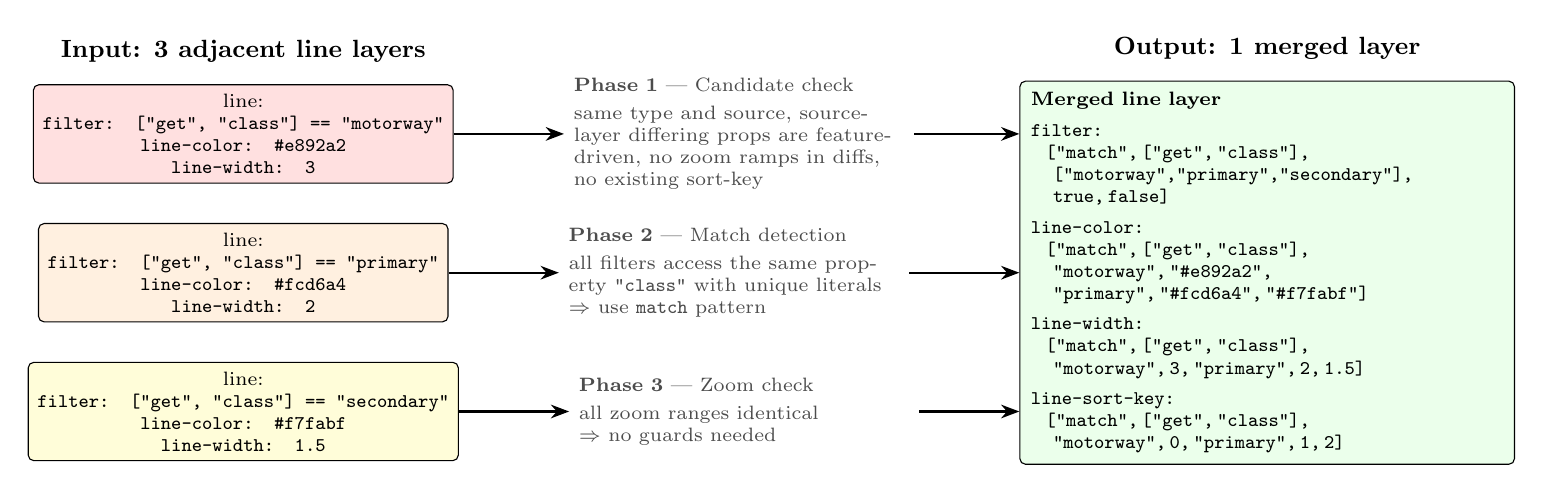
\begin{tikzpicture}[
        node distance=0.35cm,
        layer/.style={rectangle, draw, rounded corners=2pt, minimum width=3.2cm,
                      minimum height=0.55cm, font=\scriptsize, align=center},
        merged/.style={rectangle, draw, rounded corners=2pt, minimum width=4.8cm,
                       font=\scriptsize, align=left, inner sep=4pt},
        phase/.style={rectangle, draw, dashed, rounded corners=3pt, fill=gray!8,
                      inner sep=5pt},
        arrow/.style={-Stealth, thick},
        label/.style={font=\scriptsize\itshape, text=gray},
        check/.style={font=\scriptsize, text=black!70},
    ]
        % Input layers (left)
        \node[layer, fill=red!12]   (l0) {line:\\ \texttt{filter: ["get", "class"] == "motorway"}\\\texttt{line-color: \#e892a2}\\\texttt{line-width: 3}};
        \node[layer, fill=orange!12, below=0.5cm of l0] (l1) {line:\\\texttt{filter: ["get", "class"] == "primary"}\\\texttt{line-color: \#fcd6a4}\\\texttt{line-width: 2}};
        \node[layer, fill=yellow!15, below=0.5cm of l1] (l2) {line:\\\texttt{filter: ["get", "class"] == "secondary"}\\\texttt{line-color: \#f7fabf}\\\texttt{line-width: 1.5}};

        \node[above=0.15cm of l0, font=\small\bfseries] {Input: 3 adjacent line layers};

        % Phase annotations (middle)
        \node[right=1.4cm of l0, check, text width=4.2cm] (p1) {%
            \textbf{Phase 1} — Candidate check\\[2pt]
            same type and source,
            source-layer differing props are feature-driven,
            no zoom ramps in diffs,
            no existing sort-key};
        \node[right=1.4cm of l1, check, text width=4.2cm] (p2) {%
            \textbf{Phase 2} — Match detection\\[2pt]
            all filters access the same property \texttt{"class"} with unique literals\\
            $\Rightarrow$ use \texttt{match} pattern};
        \node[right=1.4cm of l2, check, text width=4.2cm] (p3) {%
            \textbf{Phase 3} — Zoom check\\[2pt]
            all zoom ranges identical\\
            $\Rightarrow$ no guards needed};

        % Output (right)
        \node[merged, fill=green!8, right=1.4cm of p2, text width=6.0cm] (out) {%
            \textbf{Merged line layer}\\[3pt]
            \texttt{filter:}\\
            \texttt{~~["match",\,["get",\,"class"],}\\
            \texttt{~~~["motorway","primary","secondary"],}\\
            \texttt{~~~true,\,false]}\\[3pt]
            \texttt{line-color:}\\
            \texttt{~~["match",\,["get",\,"class"],}\\
            \texttt{~~~"motorway",\,"\#e892a2",}\\
            \texttt{~~~"primary",\,"\#fcd6a4",\,"\#f7fabf"]}\\[3pt]
            \texttt{line-width:}\\
            \texttt{~~["match",\,["get",\,"class"],}\\
            \texttt{~~~"motorway",\,3,\,"primary",\,2,\,1.5]}\\[3pt]
            \texttt{line-sort-key:}\\
            \texttt{~~["match",\,["get",\,"class"],}\\
            \texttt{~~~"motorway",\,0,\,"primary",\,1,\,2]}
        };

        \node[above=0.15cm of out, font=\small\bfseries] {Output: 1 merged layer};

        % Arrows
        \draw[arrow] (l0.east) -- (p1.west);
        \draw[arrow] (l1.east) -- (p2.west);
        \draw[arrow] (l2.east) -- (p3.west);
        \draw[arrow] (p1.east) -- (out.west |- p1.east);
        \draw[arrow] (p2.east) -- (out.west);
        \draw[arrow] (p3.east) -- (out.west |- p3.east);
    \end{tikzpicture}}
    \caption[Layer merging example]{Layer merging example.  Three adjacent line layers differing only in filter literal, colour, and width are merged via the \texttt{match} pattern (Phase~2).
    The merged layer uses \texttt{["match",\,["get",\,"class"],\,\ldots]} for the filter, each differing paint property, and a synthesised sort key that preserves the original draw order.
    Phase~1 validates that all differing properties support feature-driven expressions; Phase~3 confirms identical zoom ranges, so no zoom guards are needed}
    \label{fig:layer_merge_example}
\end{figure}

\paragraph{Source zoom tightening}
After all layer-level passes, source \texttt{minzoom}/\texttt{maxzoom} bounds are tightened to the effective zoom range of the layers that reference each source.
This is a liveness analysis: a source is \enquote{live} at a zoom level only if at least one layer referencing it is active at that zoom.
Tighter source bounds allow the tile server (or client-side tile manager) to skip tile requests for zoom levels where no layer needs data from that source.

\subsubsection{Data-Level Optimisations}\label{sub_data_optimisations}

Data-level optimisations transform the tile data itself, reducing transfer size and decoding cost without altering the rendered output.
\cref{tab:data_passes} summarises the implemented techniques.

\begin{table}[htbp]
\centering
\begin{tblr}{
  colspec = {p{3.8cm} p{1.8cm} p{9.5cm}},
  rows = {font=\small},
  row{1} = {font=\small\bfseries},
}
\toprule
Pass & Data & Description [compiler analogy] \\
\midrule
Tile shaving             & full scan & Encode only the properties, layers, and geometry types that the style actually references [tree shaking] \\
Transparent re-encoding  & full scan & Re-encode \ac{MVT} tiles into the \ac{MLT} format [instruction set translation] \\
Compression optimisations & full scan & Apply column-aware compression strategies based on data characteristics [\ac{PGO} optimisations] \\
\bottomrule
\end{tblr}
\caption{Data-level optimisations techniques.}
\label{tab:data_passes}
\end{table}

The pipeline operates in three stages that mirror the structure of a database query optimiser: \emph{logical} rewriting (what data to keep), \emph{physical} strategy selection (how to encode it), and \emph{cost-based} competition (which encoding is smallest).

\begin{enumerate}
    \item \textbf{Style-driven tile shaving} (\cref{sub_tile_shaving}): the optimised style is analysed to produce a \emph{tile pruning advisory} that specifies, per source-layer and zoom level, which properties, geometry types, and property values to retain.
    Tiles are pruned according to this advisory before encoding.
    \item \textbf{Data transformations} (\cref{sub_string_property_interning} and \cref{sub_feature_reordering}): remaining data is transformed to improve compressibility - categorical string properties are replaced by frequency-ordered integers (\emph{string interning}), and features are reordered to exploit spatial or categorical locality.
    \item \textbf{Encoding strategy selection} (\cref{sub_encoding_strategies}): the pruned, transformed data is re-encoded into \ac{MLT} using a multi-strategy competition that automatically profiles each data stream and selects the most compact encoding.
\end{enumerate}

\noindent The three stages compose: shaving narrows the column set fed to Stage~2, which in turn determines the value distributions Stage~3 sees.
Stage~3's profiler-driven candidate pruning responds to those distributions automatically - its viability tests (\texttt{rle\_is\_viable} at $\bar{r} \geq 2.0$, \texttt{delta\_is\_beneficial} when delta bit-widths beat raw, \texttt{delta\_rle\_is\_viable} at $\bar{r}_\Delta \geq 2.0$) operate on actual stream statistics, so a column whose distinct-value count drops after shaving naturally presents longer runs and triggers more compact candidates.

\paragraph{Style-Driven Tile Shaving}\label{sub_tile_shaving}

The bridge between style-level and data-level optimisations is the \emph{tile pruning advisory} - a structured report that captures, for each source-layer and zoom level, exactly what the rendering style needs.
The advisory is computed from the \emph{optimised} style (after all expression and structural passes) together with tile statistics.
This ordering is critical: style-level dead layer elimination, metadata refinement, and layer merging reduce the set of live style layers, which in turn reduces the set of referenced properties and geometry types in the advisory.
The preceding style optimisations thus feed into data-level savings, though the aggregate interaction is additive rather than synergistic (\cref{sub_mlt_results}).
This cascade mirrors the materialized-view maintenance problem described in \cref{sub_materialized_views}: the rendering style acts as the view definition, the tile set as the base relation, and the shaved tile as the materialized view.
When the style changes (e.g., dead elimination removes a layer), the advisory changes, which in turn changes the shaved output - precisely the incremental view maintenance problem of updating a derived dataset under view-definition changes.

The advisory captures the following per source-layer:

\begin{itemize}
    \item \textbf{Used properties with zoom ranges}: for each property name appearing in a \texttt{["get",~\ldots]} or \texttt{["has",~\ldots]} expression in any live style layer, the zoom range over which it is referenced.
    Properties not referenced at any zoom level are candidates for removal.
    \item \textbf{Used geometry types with zoom ranges}: which of Point, LineString, and Polygon are needed, derived from the style layer types (e.g., \texttt{fill} $\to$ Polygon, \texttt{circle} $\to$ Point).
    Features with geometry types unused by any style layer at the current zoom level are removed.
    \item \textbf{Unused zoom levels}: zoom levels at which no style layer targets the source-layer.
    Tiles at these zoom levels need not be encoded at all.
    \item \textbf{Unused property values}: specific values of categorical properties that are never matched by any style filter.
    For example, if no style layer filters for \texttt{class = "ferry"}, features with that value can be removed.
    \item \textbf{Feature ID requirement}: whether any style layer uses \texttt{["id"]} or \texttt{["feature-state",~\ldots]}.
    When IDs are unused, the entire ID column is stripped.
\end{itemize}

\noindent The pruning advisory is applied to each \ac{MVT} tile before encoding (\cref{fig:tile_shaving_pipeline}).

\begin{figure}[htbp]
    \centering
    \begin{tikzpicture}[
        box/.style={rectangle, draw, rounded corners=2pt, minimum height=0.65cm, font=\small, align=center},
        style/.style={box, fill=blue!10, minimum width=2.8cm},
        data/.style={box, fill=orange!10, minimum width=2.8cm},
        both/.style={box, fill=green!10, minimum width=2.8cm},
        arrow/.style={-Stealth, thick},
        lbl/.style={font=\scriptsize\itshape, text=gray, align=center},
        steps/.style={rectangle, draw, dashed, rounded corners=2pt, font=\small,
                      align=left, inner sep=6pt, text=black!80},
    ]
        % Row 1: style-side and data-side inputs
        \node[style] (sopt) {Style optimisations\\{\scriptsize (\cref{sub_expression_optimisations,sub_structural_optimisations})}};

        % Row 2: advisory
        \node[both, right=3cm of sopt] (adv) {Tile pruning advisory};
        \draw[arrow] (sopt) -- node[above, lbl] {optimised style} (adv);

        % Row 3:
        \node[data, right=3cm of adv] (stats) {Tile statistics};
        \draw[arrow] (stats) -- node[above, lbl] {property/\\geom distribution} (adv);

        % Row 3: MVT → prune → MLT
        \node[data, below=1.5cm of adv] (prune) {Prune \& transform};
        \node[data] at ($(sopt |- prune)$) (mvt) {\ac{MVT} tile};
        \node[data] at ($(stats |- prune)$) (mlt) {\ac{MLT} tile};

        \draw[arrow] (adv) -- (prune);
        \draw[arrow] (mvt) -- (prune);
        \draw[arrow] (prune) -- node[above, lbl] {re-encode} (mlt);

        % Pruning steps annotation
        \node[steps, below=1cm of prune] (ops) {%
            \textbf{Pruning operations (in order):}\\[2pt]
            1.\;Remove entire source-layers not referenced by any style layer.\\
            2.\;For each remaining layer:\\
            \quad a.\;Filter features by geometry type at current zoom.\\
            \quad b.\;Filter features by unused categorical property values.\\
            \quad c.\;Strip unused properties from the key-value table.\\
            \quad d.\;Strip feature IDs when not needed.%
        };
        \draw[dashed, gray] (prune) -- (ops);
    \end{tikzpicture}
    \caption{Style-driven tile shaving pipeline.  The optimised style and tile statistics jointly produce a pruning advisory.  Each \ac{MVT} tile is pruned according to the advisory, transformed, and re-encoded as \ac{MLT}.  Style-level dead layer elimination narrows the advisory, which can reduce the data that must be encoded}
    \label{fig:tile_shaving_pipeline}
\end{figure}

After pruning, two data transformations improve compressibility before encoding.

\paragraph{String property interning}\label{sub_string_property_interning}
Categorical string properties - such as road class, land-use type, or administrative level - are replaced by frequency-ordered integer indices.
The interning table is derived from the tile statistics: all distinct values of a string property are sorted by descending frequency, and each value is assigned a sequential integer starting from~0.
The most common value receives index~0, the second most common receives~1, and so on.

This transformation has two benefits.
First, it reduces the per-feature storage cost from a variable-length string (with length prefix and dictionary overhead) to a small integer (typically \qtyrange{1}{2}{\byte} as a \ac{VarInt}).
Second, the frequency ordering means that common values receive small indices, which compress well under \ac{VarInt} and delta encoding.

The corresponding style expressions are rewritten to reference the integer indices rather than the original string values.
For example, a filter \texttt{["==",~["get",~"class"],~"primary"]} is rewritten to \texttt{["==",~["get",~"class"],~0]} if \texttt{"primary"} is the most frequent value.
This rewriting ensures that the optimised style remains consistent with the transformed tile data.
Because interned tiles encode property values as style-specific integer indices rather than original strings, they are only compatible with the paired optimised style; other consumers (debugging tools, alternative renderers) would see opaque integers.
Interning is therefore an optional pipeline stage that can be disabled for multi-consumer deployments where tiles must remain self-describing.

\paragraph{Feature reordering}\label{sub_feature_reordering}
The order of features within a tile layer affects the compressibility of every parallel column.
The encoder explores multiple feature orderings - spatial (Hilbert/Morton curve of first vertex), ID-based, and property-based (grouping by a low-cardinality attribute) - and retains the ordering that produces the smallest encoded output.
This is described in detail in \cref{sub_encoding_strategies}.

The pruned and transformed data is re-encoded into the \ac{MLT} columnar format.
This is done via

\paragraph{Automatic Encoding Strategy Selection}\label{sub_encoding_strategies}
The re-encoding proceeds in three stages: (1)~the row-oriented \ac{MVT} features are converted into an owned columnar representation (\texttt{StagedLayer01}), with separate arrays for each property column, the geometry vertex buffer, and the feature ID column; (2)~the columnar data is optionally reordered according to the sort strategy competition; (3)~each column is independently encoded using the per-stream encoding competition.
The final wire format consists of three concatenated sections per layer: a header (layer name, tile extent, column count), a metadata section (column types, encoding descriptors), and a data section (the encoded streams).

The Rust-based encoder reformulates the encoding problem as a \emph{multi-strategy competition} inspired by \ac{PGO} in compilers~\cite{changUsingProfileInformation1991} and the instance-optimised systems vision of Kraska~\cite{kraskaInstanceOptimizedData2021}:
rather than committing to a single encoding plan, the encoder uses the data distribution of each tile to try multiple strategies, measures the output size of each, and selects the smallest result.
This competition operates at two nested levels: an \emph{outer loop} that trials multiple feature sort orderings, and an \emph{inner loop} that selects the best integer encoding for each individual data stream.
The inner competition criterion is deliberately \emph{single-objective}: the winning candidate is the one with the smallest encoded \texttt{total\_len()}.
Multi-axis trade-offs - between transfer size, decoding latency, rendering throughput, and preprocessing cost - are not resolved inside the encoder; they are reported separately per metric in the ablation evaluation (\cref{ch_experiments}), where the contribution of each pass can be assessed against the deployment-relevant axis.

A no-copy alternatives mechanism lets each candidate write into the encoder's buffers and rolls losing candidates back by resetting cursor positions, so the inner and outer competitions nest without redundant allocation.

\begin{figure}[htbp]
    \centering
    \begin{subfigure}[t]{0.45\linewidth}
        \centering
        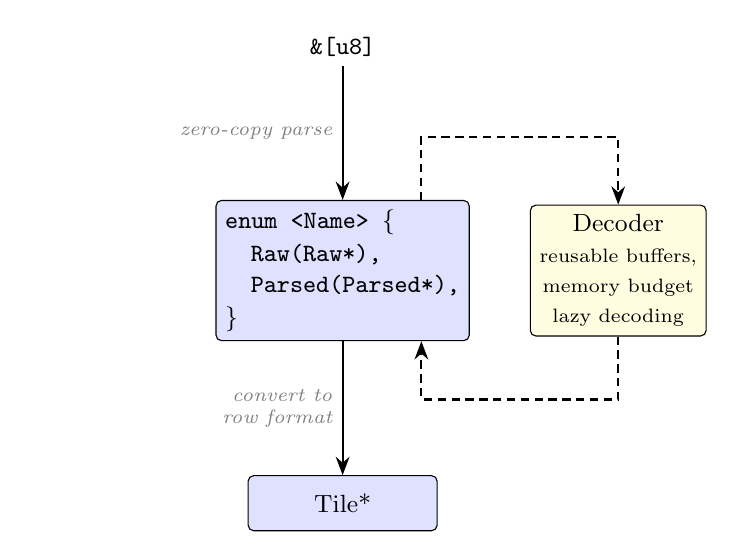
\begin{tikzpicture}[
            box/.style={rectangle, draw, rounded corners=2pt, minimum height=0.7cm,
                        minimum width=2.4cm, font=\small, align=center},
            decode/.style={box, fill=blue!12},
            dec/.style={box, fill=yellow!12, minimum width=1.6cm},
            io/.style={font=\small\ttfamily},
            arrow/.style={-Stealth, thick},
            lbl/.style={font=\scriptsize\itshape, text=gray},
            node distance=1.7cm,
        ]
            % Main pipeline on centre line (x=0)
            \node[io]     (u8)     {\&[u8]};
            \node[decode, below=of u8, minimum width=3.2cm, align=left]     (name)
                {\texttt{enum <Name> \{}\\[1pt]\quad\texttt{Raw(Raw*),}\\[0pt]\quad\texttt{Parsed(Parsed*),}\\[1pt]\texttt{\}}};
            \draw[arrow] (u8)   -- node[left, lbl, align=right] {zero-copy parse} (name);
            \node[decode, below=of name] (tile)   {Tile*};
            \draw[arrow] (name) -- node[left, lbl, align=right] {convert to\\row format} (tile);

            % Decoder off-centre towards the middle (right side)
            \node[dec, right=3.5cm of name.center, anchor=center] (decnode)
            {Decoder\\{\scriptsize reusable buffers,}\\{\scriptsize memory budget}\\{\scriptsize lazy decoding}};
            \draw[-Stealth, thick, densely dashed]
            ($(name.north) + (1,0)$) -- ++(0,0.8) -| (decnode.north);
            \draw[-Stealth, thick, densely dashed]
            (decnode.south) -- ++(0,-0.8) -| ($(name.south) + (1,0)$);

            % Phantom to balance bounding box
            \path (-4, 0);

            % Decoder arrows
        \end{tikzpicture}
        \caption{Decoding pipeline: An input \texttt{\&[u8]} slice is zero-copy parsed into a \texttt{<Name>} container whose columns are held as \texttt{Raw,\,Parsed} variants, decoded on demand. columnar data can then be converted to row-oriented \texttt{Tile*} features as needed.}
        \label{fig:arch_dec_sub}
    \end{subfigure}
    \hfill
    \begin{subfigure}[t]{0.45\linewidth}
        \centering
        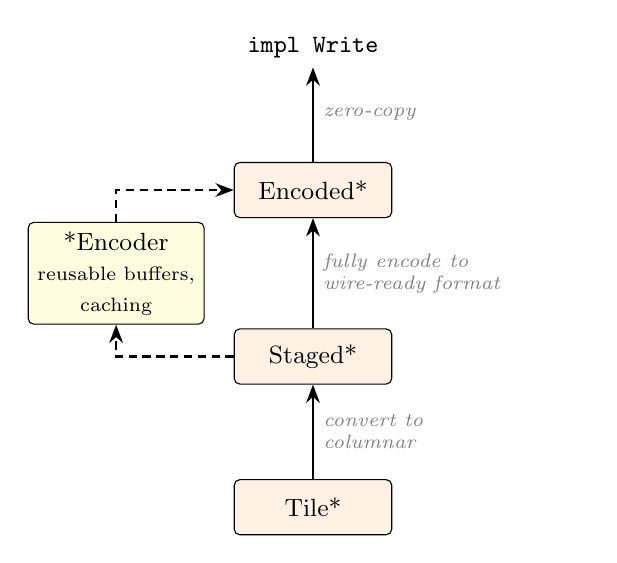
\begin{tikzpicture}[
            box/.style={rectangle, draw, rounded corners=2pt, minimum height=0.7cm,
                        minimum width=2.0cm, font=\small, align=center},
            encode/.style={box, fill=orange!10},
            enc/.style={box, fill=yellow!12, minimum width=1.6cm},
            io/.style={font=\small\ttfamily},
            arrow/.style={-Stealth, thick},
            lbl/.style={font=\scriptsize\itshape, text=gray},
            node distance=1.2cm,
        ]
            % Main pipeline on centre line (x=0)
            \node[io]     (write)   {impl Write};
            \node[encode, below=of write]   (encoded) {Encoded*};
            \node[encode, below=1.4cm of encoded] (staged)  {Staged*};
            \node[encode, below=of staged]  (tile)    {Tile*};

            % *Encoder off-centre towards the middle (left side)
            \node[enc] at ($(staged)!0.5!(encoded) + (-2.5,0)$) (encnode) {*Encoder\\{\scriptsize reusable buffers,}\\{\scriptsize caching}};

            \draw[arrow] (tile)    -- node[right, lbl, align=left] {convert to\\columnar} (staged);
            \draw[arrow] (staged)  -- node[right, lbl, align=left] {fully encode to\\wire-ready format} (encoded);
            \draw[arrow] (encoded) -- node[right, lbl] {zero-copy} (write);

            % Phantom to balance bounding box
            \path (3.5, 0);

            % Encoder arrows
            \draw[-Stealth, thick, densely dashed] (staged.west) -| (encnode.south);
            \draw[-Stealth, thick, densely dashed] (encnode.north) |- (encoded.west);
        \end{tikzpicture}
        \caption{Encoding pipeline: Row-oriented \texttt{Tile*} features are converted to columnar \texttt{Staged*} data, fully encoded to wire-ready \texttt{Encoded*} byte buffers via \texttt{*Encoder} types that implement the multi-strategy competition, and written to an \texttt{impl Write} sink via a final zero-copy step.}
        \label{fig:arch_enc_sub}
    \end{subfigure}
    \caption{Encoder~\subref{fig:arch_enc_sub} and decoder~\subref{fig:arch_dec_sub} data-flow in \texttt{mlt-core}}
    \label{fig:arch_enc}
\end{figure}

In an outer loop, a sort-strategy competition is run.
Reordering features within a layer permutes every parallel column - geometry, IDs, and all properties - simultaneously.
Different orderings favour different encoding schemes: spatial orderings cluster nearby geometries and their correlated properties, improving \ac{RLE} run lengths; ID ordering produces sequential integer sequences amenable to delta-\acs{RLE}.
Which ordering wins depends on the value distributions and cardinalities of the specific layer: a layer dominated by a single repeated property value may benefit most from spatial clustering, while a layer with sequential IDs and high-cardinality properties may favour ID ordering.
Because this balance shifts across layers, zoom levels, and tilesets, no single ordering dominates universally, and the choice cannot be resolved statically.

The encoder therefore trials multiple sort strategies on the same data and retains the encoding with the smallest total byte count.
The implemented strategies and their rationale are:

\begin{enumerate}
    \item \textbf{Unsorted}: the original feature order is preserved.
    \item \textbf{Spatial (Morton/Z-order)}: features are sorted by the Z-order curve index of their first vertex, computed via bit-interleaving.  Fast to compute; provides reasonable spatial locality.
    \item \textbf{Spatial (Hilbert)}: features are sorted by the Hilbert curve index of their first vertex.  Slower to compute than Morton but achieves superior spatial locality, as the Hilbert curve avoids the long jumps inherent in the Z-order curve's recursive structure~\cite{moonAnalysisClusteringProperties2001}.
    \item \textbf{ID}: features are sorted by feature ID in ascending order.
\end{enumerate}

For each candidate strategy, the encoder constructs a fresh \texttt{Encoder} instance, encodes the reordered layer, and measures the total output size (header + metadata + data).
The strategy producing the smallest output is retained; all others are discarded.
When only a single strategy is applicable, the competition is elided and the layer is encoded directly without cloning.
Property-based sort strategies were considered but are not included in the current implementation, because the string interning pass (\cref{sub_string_property_interning}) already groups features of the same discriminator value into dense dictionary-index ranges, and Hilbert or ID ordering strictly dominated an explicit categorical sort on the benchmark tileset.

\begin{figure}[htbp]
    \centering
    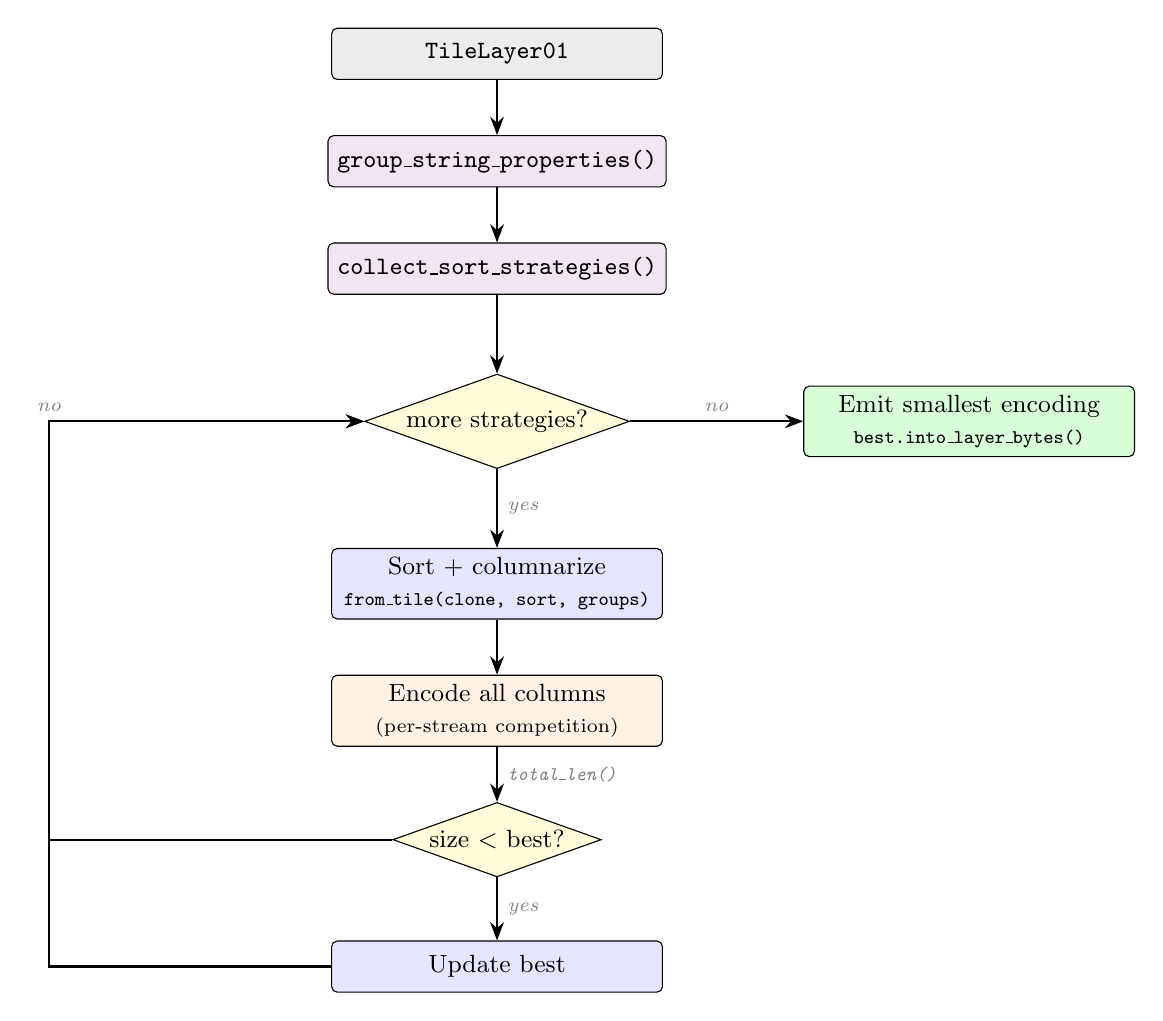
\begin{tikzpicture}[
        node distance=0.7cm,
        box/.style={rectangle, draw, rounded corners=2pt, minimum width=4.2cm,
            minimum height=0.65cm, font=\small, align=center},
        input/.style={box, fill=gray!15},
        prep/.style={box, fill=violet!10},
        stage/.style={box, fill=blue!10},
        encoder/.style={box, fill=orange!10},
        decision/.style={diamond, draw, fill=yellow!15, aspect=2.8,
            font=\small, inner sep=1pt},
        output/.style={box, fill=green!15},
        arrow/.style={-Stealth, thick},
        label/.style={font=\scriptsize\itshape, text=gray},
        ]
        % Input
        \node[input] (layer) {\texttt{TileLayer01}};

        % Prep: group_string_properties
        \node[prep, below=of layer] (grp)
        {\texttt{group\_string\_properties()}};
        \draw[arrow] (layer) -- (grp);

        % Prep: collect_sort_strategies
        \node[prep, below=of grp] (coll)
        {\texttt{collect\_sort\_strategies()}};
        \draw[arrow] (grp) -- (coll);

        % Loop guard
        \node[decision, below=1.0cm of coll] (more) {more strategies?};
        \draw[arrow] (coll) -- (more);

        % Sort + columnarize
        \node[stage, below=1.0cm of more] (sort)
        {Sort + columnarize\\%
            {\scriptsize\texttt{from\_tile(clone, sort, groups)}}};
        \draw[arrow] (more) -- node[right, label] {yes} (sort);

        % Encode
        \node[encoder, below=of sort] (enc)
        {Encode all columns\\{\scriptsize (per-stream competition)}};
        \draw[arrow] (sort) -- (enc);

        % Compare
        \node[decision, below=of enc] (cmp) {size $<$ best?};
        \draw[arrow] (enc) -- node[right, label] {\texttt{total\_len()}} (cmp);

        % Yes: update best, then loop back
        \node[stage, below=0.8cm of cmp] (upd) {Update best};
        \draw[arrow] (cmp) -- node[right, label] {yes} (upd);

        % No: discard, loop back
        \draw[arrow] (upd.west) -| ($(more.west)+(-4cm,0)$) |- node[above, label] {no} (more.west);
        \draw[arrow] (cmp.west) -| ($(more.west)+(-4cm,0)$) |- (more.west);

        % Exit loop
        \node[output, right=2.2cm of more] (best) {Emit smallest encoding\\{\scriptsize\texttt{best.into\_layer\_bytes()}}};
        \draw[arrow] (more.east) -- node[above, label] {no} (best.west);
    \end{tikzpicture}
    \caption{Multi-strategy sort competition.
        Shared-dictionary string groups are computed once and reused across all trials.
        The encoder collects candidate sort strategies, pruning spatial strategies via the bounding-box heuristic for large, widely-spread layers.
        For each candidate, the layer is cloned, sorted, and columnarized via \texttt{from\_tile}; the columnar data is then encoded with per-stream integer competitions.
        The encoding with the smallest \texttt{total\_len()} is retained}
    \label{fig:sort_competition}
\end{figure}

To avoid wasting trials on unpromising strategies, a \emph{bounding-box heuristic} skips spatial sorting on large layers whose features are too spatially dispersed for locality clustering to help.
Specifically, for layers with more than \texttt{512} features, the spatial trials are pruned when the first-vertex bounding box covers more than \texttt{80\%} of the tile extent on \emph{both} axes.
Small layers (below the threshold) are always trialled, since the absolute cost of an extra encoding pass is negligible for them.
The thresholds were experimentally derived from Germany-wide OpenMapTiles.

In an inner loop, a per-stream encoding competition trials every viable integer encoding for the data stream .
Each candidate pairs a \emph{logical} encoding (Plain, Delta, \ac{RLE}, or DeltaRle) with a \emph{physical} encoding (\ac{VarInt} or \ac{FastPFOR}~\cite{lemireDecodingBillionsIntegers2015}).
The general stream competition currently covers these four logical encodings; geometry-specific strategies (Morton-delta, componentwise-delta) are applied via a separate encoding path optimised for coordinate data, since their semantics are tied to the two-dimensional structure of vertex sequences and do not generalise to property columns.
Extending the general competition to include additional strategies (e.g., frame-of-reference without delta, or hybrid schemes) is a direction for future work, though the current candidate set captures the dominant encoding patterns observed in the benchmark tileset.
The na\"ive approach - encoding every combination and comparing - would be prohibitively expensive for large tiles.
Instead, a \emph{data profiler} samples a contiguous block taken from the middle of the stream: streams with at most $512$ values are profiled in full, and longer streams are profiled over $\lfloor |s| / 100 \rfloor$ values clamped to $[512,\, 16384]$.
The contiguous mid-stream window is chosen over a random sample because \ac{RLE} run lengths and delta-bit-width statistics are destroyed by permutation, and because the middle of a spatially or ID-sorted stream is a representative point away from the boundary artefacts at the ends.
The profiler computes four metrics in a single pass:

\begin{itemize}
    \item \emph{Average run length} ($\bar{r} = |s| / n_{\text{runs}}$): the mean number of consecutive identical values.
    \item \emph{Delta average run length} ($\bar{r}_\Delta = (|s|-1) / n_{\Delta\text{-runs}}$): the mean run length in the zigzag-encoded delta stream.
    \item \emph{Sortedness}: whether the sample is monotonically ascending or descending.
    \item \emph{Bit-width sums}: the total bit widths of both raw values and zigzag-encoded deltas, used to estimate whether delta encoding reduces the representation cost.
\end{itemize}

Based on these metrics, candidates are pruned before any full encoding is attempted:
\ac{RLE} is excluded when $\bar{r} < 2.0$;
Delta is excluded when the stream is unsorted \emph{and} delta bit widths exceed raw bit widths;
DeltaRle is excluded when $\bar{r}_\Delta < 2.0$ and neither \ac{RLE} nor Delta is independently viable.
\ac{FastPFOR} is only offered for 32-bit integer types, as the algorithm's block structure is designed for fixed-width words.
The remaining candidates (typically two to four) are encoded in full, and the smallest output is committed.

\paragraph{String encoding}
String columns are competed across four strategies, reflecting the two orthogonal dimensions of string compression: deduplication and byte-level compression.

\begin{enumerate}
    \item \textbf{Plain}: raw bytes with length prefixes.
    The length stream is itself subject to the integer encoding competition.
    \item \textbf{Dictionary}: a deduplicated corpus with per-string offset indices.
    Effective when many features share the same string value (e.g., road names that repeat across tiles).
    \item \textbf{\ac{FSST}}~\cite{bonczFSSTFastRandom2020}: a lightweight, random-access string compressor that learns a symbol table of up to~255 frequent byte sequences and replaces occurrences with single-byte codes.
    The symbol table is stored once per column; the compressed corpus remains directly scannable without decompression.
    \item \textbf{\ac{FSST} + Dictionary}: \ac{FSST} applied to a deduplicated dictionary, combining both deduplication and byte-level compression.
\end{enumerate}

A viability probe ensures that \ac{FSST} is only attempted when the symbol-table overhead (up to \qty{2040}{\byte}) is likely to be recouped: columns below \num{2048}~raw bytes are excluded, and a trial compression on a sample of up to \num{256} strings is evaluated before committing.
Trained \ac{FSST} compressors are cached by column name in a \texttt{HashMap} and reused across all sort-strategy trials, avoiding redundant training.
A \emph{pruning variant} of the \ac{FSST} compressor removes symbols whose observed frequency in the trial compression falls below a viability threshold, shrinking the stored symbol table at no additional decoder cost.

\paragraph{Shared dictionary grouping}\label{sub_cardinality}
The \ac{MLT} format supports shared dictionaries where multiple string columns reference a common deduplicated corpus, amortising dictionary overhead across columns with overlapping vocabularies.
The prior Java encoder groups columns by naming prefix (e.g., \texttt{name}, \texttt{name:en}, \texttt{name:de}), which misses semantic overlaps (e.g., \texttt{class} and \texttt{subclass} in OpenMapTiles share many values).

\begin{sloppypar}
    The Rust encoder replaces prefix matching with -based similarity clustering~\cite{broderResemblanceContainmentDocuments1998}.
    For each string column, two MinHash sketches of $128$ permutations are computed: one over exact string values and one over byte trigrams (3-byte sliding windows).
    The choice of 128 permutations corresponds to an expected standard error of approximately $1/\sqrt{128} \approx 8.8\%$ on the Jaccard estimate, which is adequate for the binary accept/reject decision of the clustering step.
    The trigram sketch captures partial overlap between columns whose values are substrings or morphological variants of each other.
    Pairwise Jaccard similarity is estimated as $\hat{J} = |\{i : h_i^{(a)} = h_i^{(b)}\}| / 128$ for each sketch type, and the maximum of two estimates is taken.
    Columns whose similarity exceeds \texttt{7.5\%} are unified via a Union-Find structure (union by size); the low threshold reflects that even small vocabulary overlap reduces the marginal cost of adding a column to an existing dictionary.
    Groups with fewer than two members are discarded.
    The threshold and similarity mode were selected via a sweep over $[2.5\%, 20\%]$ under three similarity modes (\emph{hybrid} taking $\max(\textit{exact}, \textit{trigram})$, \emph{only-trigram}, \emph{only-exact}), applied to the Germany OpenMapTiles tileset and measuring the total encoded size after clustering (\cref{fig:minhash_sweep}; the sweep harness is \texttt{scripts/generate\_minhash\_sweep.py}, which patches the threshold constant, rebuilds the encoder, and re-encodes the tileset for each cell).
    All three modes produce monotonically smaller output as the threshold decreases (i.e.\ as more column pairs qualify for grouping), with hybrid mode producing the smallest output at every threshold.
    The total spread across all 15 cells is approximately \qty{6}{\mega\byte} ($\approx \qty{0.19}{\percent}$ of the \qty{3.14}{\giga\byte} tileset), indicating that shared-dictionary grouping has a measurable but modest effect on total encoded size.
    The hybrid mode at 0.025 yields the overall minimum; however, the marginal improvement from 0.075 to 0.025 is only \qty{1.6}{\mega\byte}, and lower thresholds increase the risk of false-positive unions on tilesets with different vocabulary distributions.
    The value 0.075 is therefore retained as a conservative default that captures the majority of the grouping benefit while leaving headroom for datasets where column vocabularies are less correlated than in OpenMapTiles.
\end{sloppypar}

\DeclareRobustCommand{\circled}[1]{\tikz[baseline=(char.base)]{\node[circle, draw, inner sep=1pt, font=\scriptsize\bfseries] (char) {#1};}}

\begin{figure}[htbp]
    \centering
    \resizebox{\textwidth}{!}{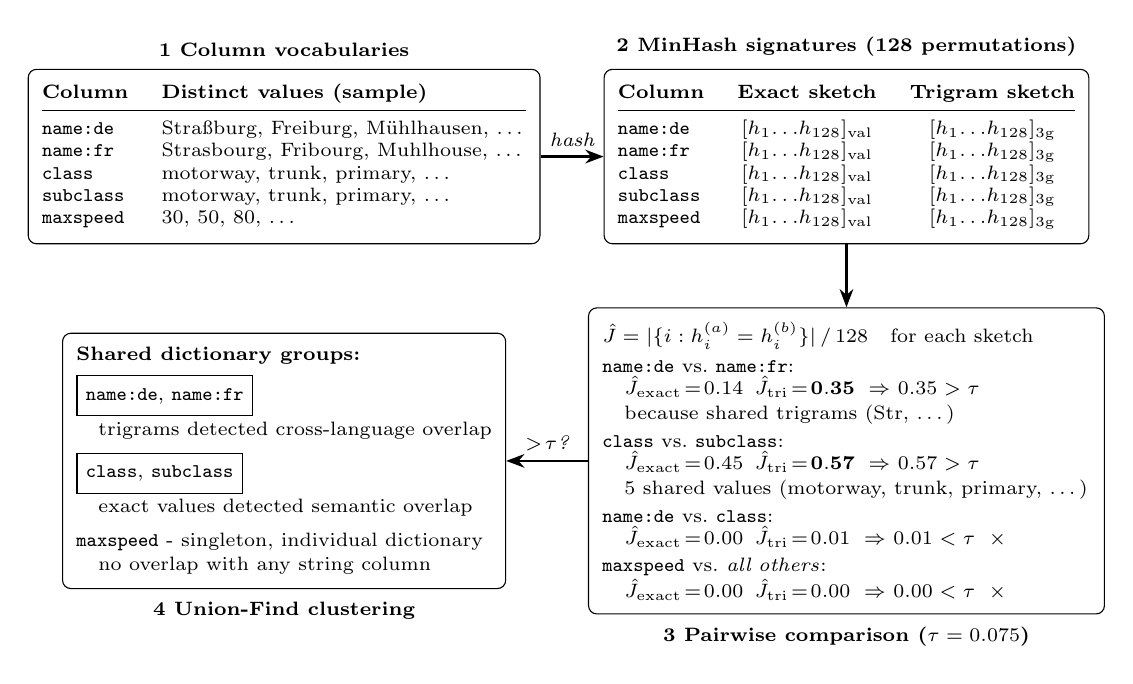
\begin{tikzpicture}[
            arrow/.style={-Stealth, thick},
            cmp/.style={font=\scriptsize, align=left},
            stepbox/.style={draw, rounded corners=3pt, inner sep=5pt, font=\scriptsize},
            steplabel/.style={font=\scriptsize\bfseries},
            ]
            % Top-left (Step 1): Column value table
            \node[stepbox] (tbl) {%
                \begin{tabular}{@{}l l@{}}
                    \textbf{Column} & \textbf{Distinct values (sample)} \\
                    \midrule
                    \texttt{name:de}  & Straßburg, Freiburg, Mühlhausen, \ldots \\
                    \texttt{name:fr}  & Strasbourg, Fribourg, Muhlhouse, \ldots \\
                    \texttt{class}    & motorway, trunk, primary, \ldots \\
                    \texttt{subclass} & motorway, trunk, primary, \ldots \\
                    \texttt{maxspeed} & 30, 50, 80, \ldots
                \end{tabular}%
            };
            \node[steplabel, above=1pt of tbl] {\circled{1} Column vocabularies};

            % Top-right (Step 2): MinHash sketch generation
            \node[stepbox, right=0.8cm of tbl, anchor=west] (hash) {%
                \begin{tabular}{@{}l c c@{}}
                    \textbf{Column} & \textbf{Exact sketch} & \textbf{Trigram sketch} \\
                    \midrule
                    \texttt{name:de}  & $[h_1\!\ldots\!h_{128}]_{\text{val}}$ & $[h_1\!\ldots\!h_{128}]_{\text{3g}}$ \\
                    \texttt{name:fr}  & $[h_1\!\ldots\!h_{128}]_{\text{val}}$ & $[h_1\!\ldots\!h_{128}]_{\text{3g}}$ \\
                    \texttt{class}    & $[h_1\!\ldots\!h_{128}]_{\text{val}}$ & $[h_1\!\ldots\!h_{128}]_{\text{3g}}$ \\
                    \texttt{subclass} & $[h_1\!\ldots\!h_{128}]_{\text{val}}$ & $[h_1\!\ldots\!h_{128}]_{\text{3g}}$ \\
                    \texttt{maxspeed} & $[h_1\!\ldots\!h_{128}]_{\text{val}}$ & $[h_1\!\ldots\!h_{128}]_{\text{3g}}$ \\
                \end{tabular}%
            };
            \node[steplabel, above=1pt of hash] {\circled{2} MinHash signatures (128 permutations)};

            % Bottom-right (Step 3): Pairwise Jaccard
            \node[stepbox, below=0.8cm of hash, cmp, text width=6.2cm, anchor=north] (sim) {%
            	$\hat{J} = |\{i : h_i^{(a)} = h_i^{(b)}\}| \,/\, 128$\quad for each sketch\\[3pt]
            	\texttt{name:de} vs.\ \texttt{name:fr}:\\
            	\quad $\hat{J}_{\text{exact}}\!=\!0.14$\enspace
            	$\hat{J}_{\text{tri}}\!=\!\mathbf{0.35}$
            	\;$\Rightarrow$ $0.35 > \tau$ \;\checkmark\\[1pt]
            	\quad{\scriptsize because shared trigrams (Str, \ldots)}\\[2pt]
            	\texttt{class} vs.\ \texttt{subclass}:\\
            	\quad $\hat{J}_{\text{exact}}\!=\!0.45$\enspace
            	$\hat{J}_{\text{tri}}\!=\!\mathbf{0.57}$
            	\;$\Rightarrow$ $0.57 > \tau$ \;\checkmark\\[1pt]
            	\quad{\scriptsize 5 shared values (motorway, trunk, primary, \ldots)}\\[2pt]
            	\texttt{name:de} vs.\ \texttt{class}:\\
            	\quad $\hat{J}_{\text{exact}}\!=\!0.00$\enspace
            	$\hat{J}_{\text{tri}}\!=\!0.01$
            	\;$\Rightarrow$ $0.01 < \tau$ \;$\times$\\[2pt]
            	\texttt{maxspeed} vs.\ \emph{all others}:\\
            	\quad $\hat{J}_{\text{exact}}\!=\!0.00$\enspace
            	$\hat{J}_{\text{tri}}\!=\!0.00$
            	\;$\Rightarrow$ $0.00 < \tau$ \;$\times$%
            };
            \node[steplabel, below=1pt of sim] {\circled{3} Pairwise comparison ($\tau = 0.075$)};

            % Bottom-left (Step 4): Union-Find result
            \node[stepbox, cmp] at ($(tbl |- sim)$)  (res) {%
                \textbf{Shared dictionary groups:}\\[3pt]
                \fbox{\strut\texttt{name:de}, \texttt{name:fr}}\\[1pt]
                \quad{\scriptsize trigrams detected cross-language overlap}\\[4pt]
                \fbox{\strut\texttt{class}, \texttt{subclass}}\\[1pt]
                \quad{\scriptsize exact values detected semantic overlap}\\[4pt]
                \texttt{maxspeed} - singleton, individual dictionary\\[1pt]
                \quad{\scriptsize no overlap with any string column}%
            };
            \node[steplabel, below=1pt of res] {\circled{4} Union-Find clustering};

            % Arrows (clockwise)
            \draw[arrow] (tbl) -- node[above, font=\scriptsize\itshape] {hash} (hash);
            \draw[arrow] (hash) -- (sim);
            \draw[arrow] (sim) -- node[above, font=\scriptsize\itshape] {$>\!\tau$?} (res);

    \end{tikzpicture}}
    \caption[MinHash-based shared dictionary clustering]{MinHash-based shared dictionary clustering (clockwise from top-left).
        \circled{1}~Each string column's distinct values form a set.
        \circled{2}~Two 128-permutation MinHash sketches are computed per column: one over exact string values, one over byte trigrams (3-byte sliding windows).
        \circled{3}~Pairwise Jaccard similarity is estimated by counting matching hash positions; the maximum of the two sketch types is compared against threshold $\tau = 0.075$.
        Exact matching detects columns that share literal values (\texttt{class}/\texttt{subclass}); trigram matching detects cross-language morphological variants (\texttt{name:de}/\texttt{name:fr} in a border region).
        \circled{4}~Column pairs exceeding the threshold are unified via Union-Find; the resulting groups share a single deduplicated dictionary corpus}
    \label{fig:minhash_clustering}
\end{figure}

\begin{figure}[htbp]
    \centering
    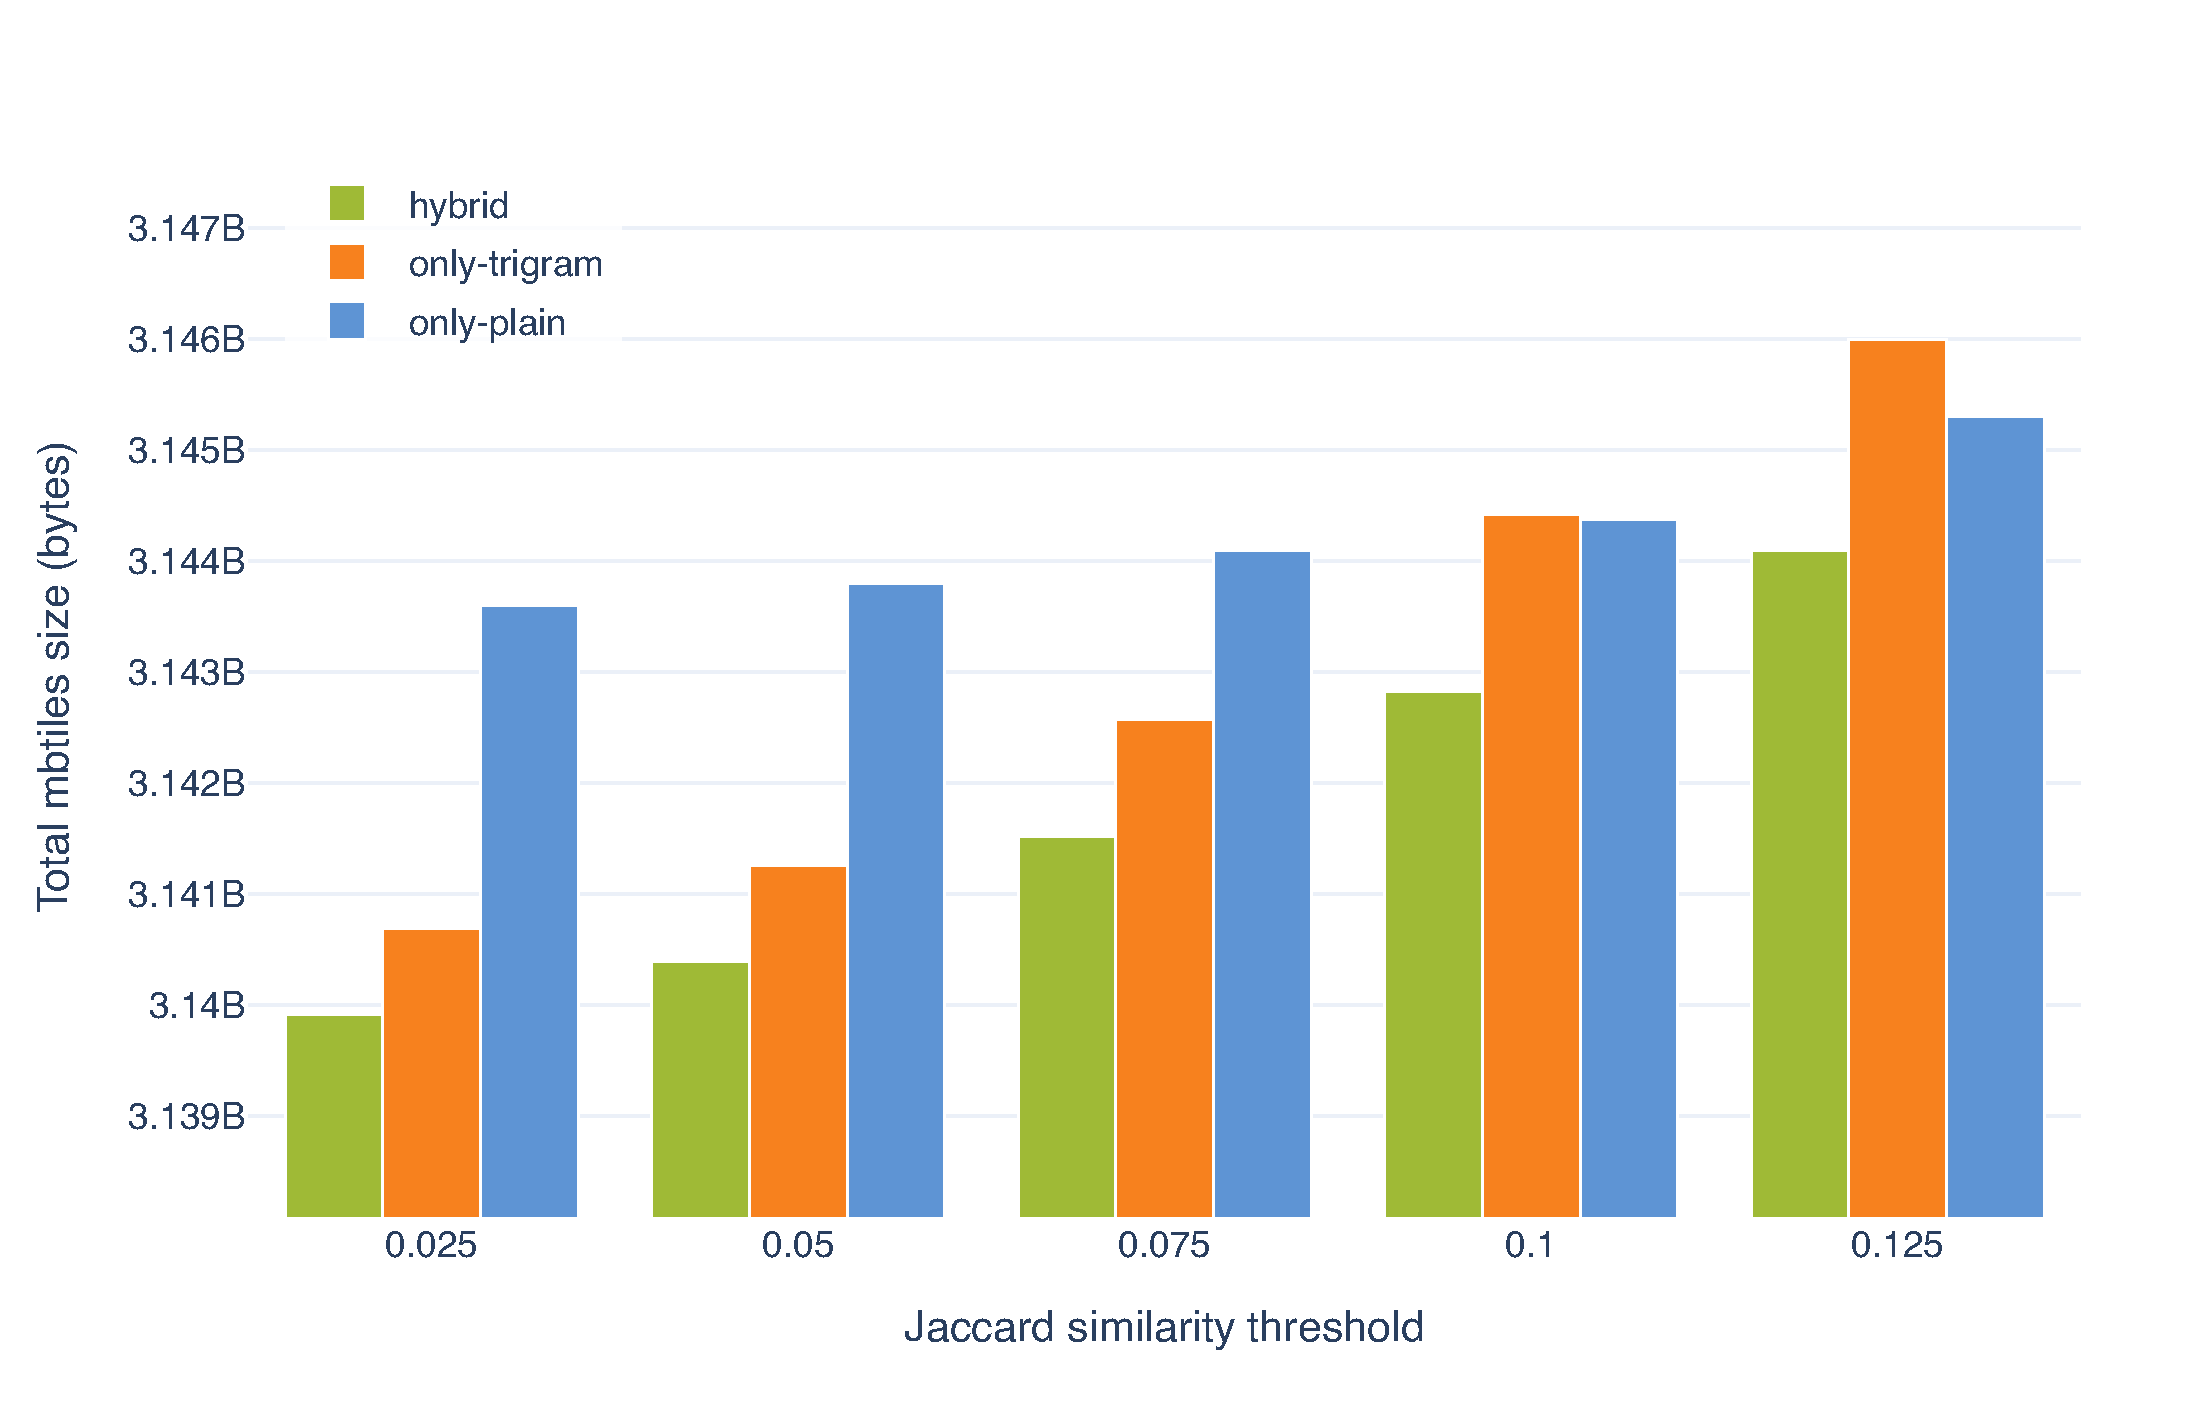
\includegraphics[width=\linewidth]{figures/minhash_sweep.pdf}
    \caption{Total encoded mbtiles size of the Germany OpenMapTiles tileset under different MinHash similarity modes and Jaccard thresholds.  Lower is better.  The hybrid mode (teal) produces the smallest output at every threshold; all modes increase monotonically with threshold as fewer column pairs qualify for shared-dictionary grouping.  The y-axis is zoomed to the data range to make the differences visible; the full range spans approximately \qty{6}{\mega\byte} out of \qty{3.14}{\giga\byte} total}
    \label{fig:minhash_sweep}
\end{figure}

\paragraph{Geometry and ID encoding}
Geometry vertices are encoded as either \emph{componentwise deltas} (CWD) or \emph{Morton-code dictionaries}.
CWD encodes each vertex as the delta from the previous vertex, producing a single interleaved stream $[x_0, y_0, \Delta x_1, \Delta y_1, \ldots]$ that is then compressed via the per-stream integer competition.
The Morton-code dictionary approach computes a Z-order code for each unique vertex pair, stores the deduplicated codes as a sorted dictionary, and references them via per-vertex offset indices - producing two streams (offsets and dictionary deltas) instead of one.
The encoder tries both strategies (when the coordinate range permits Morton encoding, i.e., both axes fit within 16~bits after shifting) and retains the smaller result.
Feature IDs are encoded through the same per-stream integer competition as other integer columns, using an explicit \texttt{IdWidth} tag (\texttt{Id32} or \texttt{Id64}) to select the physical word width.
The \ac{FastPFOR} codec operates on 32-bit blocks by construction, so only 32-bit ID streams and property columns reach it; 64-bit streams fall back to \ac{VarInt} (the \ac{VarInt} candidate list covers both widths).
The encoder chooses \texttt{Id32} when the maximum observed ID fits in \texttt{u32}, narrowing 64-bit-declared ID columns whose actual values fit in 32 bits; the round-trip correctness of this narrowing is covered by per-case tests including \texttt{test\_config\_produces\_correct\_variant} and proptest round-trips over $[0,\,\texttt{u32::MAX}]$ and $[0,\,\texttt{u64::MAX}]$ domains.
Structural patterns (sequential, constant) are discovered by the same data profiler that drives the inner competition: sequential IDs reach DeltaRle, constant IDs reach \ac{RLE}, and short or irregular sequences fall back to plain \ac{VarInt}.

\paragraph{Encoder cost amortisation}
Multi-trial encoding is made affordable through warm-start caching - \ac{FSST} compressors, Morton metadata, and vertex-strategy decisions are computed once and reused across sort trials.
Furtermore, scratch buffers grow on first use and are recycled.

The alternatives mechanism is an RAII stack of \texttt{AltSession} guards: each candidate writes into a sub-range of the encoder's buffers, and the guard's \texttt{Drop} impl retains only the bytes of the smallest candidate and rolls the cursor back for the others, so nesting lets the inner per-stream competition resolve before the enclosing sort-strategy trial commits.

\paragraph{Encoder correctness validation}
\begin{sloppypar}
    Because \ac{FastPFOR} explicitly disclaims input validation and the encoder performs narrowing, run-encoding, and dictionary rebuilds that each have independent failure modes, the encoder is validated by a multi-layer test harness:
    (i)~an in-tree proptest suite covering every \texttt{IntEncoder} variant, with round-trip assertions across the full representable range of the selected physical type;
    (ii)~a libFuzzer harness that fuzzes full \texttt{DecodedLayer} round-trips, with a corpus accumulated over previous runs;
    (iii)~snapshot tests via \texttt{insta} for the per-stream profiler's candidate lists, pinning the pruning heuristics to known-good outputs; and
    (iv)~the pixel-exact visual validation described in \cref{sec_visual_correctness}, which exercises the full decode path against a known-good baseline.
\end{sloppypar}

\subsection{Metadata Optimisations}\label{sub_metadata_optimisations}

Metadata optimisations provide the client with more accurate information, enabling it to skip unnecessary work during rendering.
\cref{tab:metadata_passes} summarises the implemented techniques.

\begin{table}[htbp]
    \centering
    \begin{tblr}{
            colspec = {p{3.8cm} p{1.8cm} p{9.5cm}},
            rows = {font=\small},
            row{1} = {font=\small\bfseries},
        }
        \toprule
        Pass & Data & Description \\
        \midrule
        Dead source elimination & none      & Remove sources that are no longer referenced after dead layer elimination \\
        Metadata refinement     & sampling  & Provide accurate \texttt{minzoom}/\texttt{maxzoom} bounds derived from filter analysis and tile statistics \\
        \bottomrule
    \end{tblr}
    \caption{Metadata-level optimisations techniques.}
    \label{tab:metadata_passes}
\end{table}

\subsection{Tile Statistics Collection}\label{sub_tile_statistics}

Several optimisations passes - stats-driven constant folding, dead elimination with geometry-type mismatch, metadata refinement, selectivity reordering, and the tile pruning advisory - require knowledge of the actual tile data.
This knowledge is provided by a statistics collection phase that scans the tile set and produces a per-source, per-source-layer statistical profile.

For each source layer, the following statistics are collected:

\begin{itemize}
    \item \textbf{Feature count}: total number of features across all tiles (note: features appearing in multiple tiles at different zoom levels are counted multiply, as the optimiser reasons per-tile, not per-geographic-entity).
    \item \textbf{Features by zoom}: a per-zoom-level feature count, used by metadata refinement to determine the first and last zoom level at which data exists.
    \item \textbf{Geometry types}: counts of Point, LineString, and Polygon features, used by dead elimination to detect geometry-type mismatches.
    \item \textbf{Feature ID presence}: whether any feature carries a non-zero feature ID, used by the advisory to decide whether to strip the ID column.
    \item \textbf{Per-property statistics}: for each property name, the statistics depend on the wire type:
    \begin{itemize}
        \item \emph{Boolean}: present count and true count.
        \item \emph{Integer/unsigned integer}: present count, minimum, maximum, cardinality, and (if cardinality $\leq 200$) a full value-frequency map.
        \item \emph{Double}: present count, minimum, maximum, cardinality (no value-frequency map, since floating-point equality is unreliable for folding).
        \item \emph{String}: present count, cardinality, and (if cardinality $\leq 200$) a value-frequency map sorted by descending frequency.
    \end{itemize}
\end{itemize}

Statistics can be collected at a configurable \emph{sample rate}.
A sample rate of~1.0 (full census) is required for irreversible decisions such as dead layer elimination or property interning; lower sample rates are sufficient for selectivity estimation and reordering.
This distinction is enforced by a sample-rate guard in the optimiser: passes that permanently remove data check that the sample rate is~1.0 before applying.

\section{Gathering a Representative Sample}\label{sec_gathering_sample}

Evaluating an optimiser requires both a diverse set of styles and realistic tile data.
We employ a two-tier strategy.

\subsection{Benchmarking Corpus}\label{sub_deep_corpus}

For rendering benchmarks that require tile data and animated camera scenarios, we curated a corpus of 15 publicly available styles that use the OpenMapTiles or BasemapDE schema:

\begin{itemize}
    \item \textbf{4 OpenFreeMap styles}: liberty, bright, positron, fiord.
    \item \textbf{7 OpenMapTiles community styles}: dark-matter, osm-bright, klokan-basic, toner, osm-liberty, americana, stadia-outdoors.
    \item \textbf{4 Government and institutional styles}: ICGC~fosc, ICGC~gris, Basemap\-DE topo\-graphic, Basemap\-DE colour.
\end{itemize}

These styles span a range of complexity-from minimal basemaps with fewer than 50~layers to verbose institutional styles with several hundred layers-and exercise different subsets of the expression language.

\subsection{Generalisation Corpus}\label{sub_generalisation_corpus}

To assess whether optimisations gains generalise beyond the deep corpus, we collected 13 styles from the Maputnik style editor catalogue (two additional catalogue entries were unavailable at the time of measurement).
These styles are evaluated using static analysis only (style size, complexity metrics, pass applicability) and do not require tile data.

\subsection{Tile Data and Caching}\label{sub_tile_data}

Tile data is sourced from \ac{OSM} via Planetiler or the German government.
Both sources are consumed through the standard Web Mercator XYZ tiling scheme used by MapLibre, so all zoom-level reasoning in the thesis assumes this grid; BasemapDE is accessed through its XYZ-compatible endpoint rather than its native \acs{WMTS} grid, ensuring that the optimiser's tile indexing is uniform across the corpus.
Only for \ac{OSM} is the underlying data fully available, so only for this source can tile statistics be collected at a sample rate of~1.0.
To ensure reproducibility across benchmark runs, all tile requests are routed through a local caching proxy that stores tiles on first access and replays them on subsequent runs with the latency and download speed of a 4G internet connection according to Rusan et al.~\cite{rusanAssessmentPacketLatency2015} ($\text{size} / 30\frac{Mb}{s} + 25ms$).
This eliminates network variability and guarantees that every ablation step operates on identical tile data (after an initial, discarded run).

All compressed-size measurements throughout this thesis use maximum compression: gzip level~9, Brotli quality~11, and zstd level~22.
This reflects the deployment scenario where tiles and styles are compressed once and served many times, so encoding cost is negligible relative to the number of requests served.

\subsection{Geographic and Use-Case Scenarios}\label{sub_scenarios}

The benchmark harness defines 18 scenarios drawn from a matrix of 15 geographic locations and 5 camera animation types:

\begin{itemize}
    \item \textbf{Locations} span high-density cities with Latin scripts (Munich, Berlin, Paris, New York, Rome), cities with non-Latin scripts (Tokyo, Beijing, Seoul, Cairo), and low-density or special nature regions (Black Forest, Amazon, Swiss Alps, Sahara, Venice, Stockholm Archipelago).
    \item \textbf{Animations} exercise different rendering workloads:
    \emph{zigzag} alternates zoom levels while panning;
    \emph{spiral} traces a circle at constant zoom with rotating bearing;
    \emph{zoomdrill} zooms from overview to street level and back;
    \emph{pansweep} sweeps across a region at constant zoom;
    \emph{bearingspin} rotates bearing at high pitch.
\end{itemize}

Each scenario is a specific (location, animation) pair.
The full cross-product of 15 locations and 5 animations is 75 pairs, which is too expensive to run for every ablation step (each cell requires 15 repeat runs for statistical validity across 17 ablation steps and 15 styles, giving roughly $75 \times 15 \times 17 \times 15 = \num{286875}$ full animations).
The 18 selected scenarios are chosen by stratified sampling so that every location appears at least once and every animation appears at least three times, and so that all combinations of density class (high/low) and script class (Latin/non-Latin) are represented.
Within each stratum the specific (location, animation) pair is the one that exercises the most layers in the densest style in the corpus, ensuring that the sample is biased \emph{against} the null hypothesis of \enquote{no effect} - i.e.\ towards scenarios where any rendering-cost differences are most likely to be visible.
This is a convenience sample by design:
it is not claimed to be unbiased across all real-world usage patterns, but it is claimed to be a reasonable stress test of the optimiser across the dimensions (density, script, zoom trajectory, camera motion) that most plausibly interact with style and data-level optimisations.

\section{Evaluation}\label{sec_evaluation}

Since many of the investigated optimisations techniques have not previously been studied in the context of map rendering pipelines, their effectiveness must be evaluated empirically.
The evaluation considers several dimensions:

\begin{itemize}
    \item \textbf{Data savings}: reduction in style size (raw, gzip, and Brotli) and tile transfer volume.
    \item \textbf{Rendering performance}: client-side metrics including load time, frames per second, frame time percentiles (p50, p95, p99), jank count, style parse time, time to first tile, and time to first frame.
    \item \textbf{Optimisation cost}: preprocessing time introduced by each pass, measured as wall-clock time on the optimiser's host machine; this is an offline cost amortised over all subsequent tile deliveries.
    \item \textbf{Efficiency}: \emph{qualitative} discussion of the energy implications of reduced data transfer and fewer rendering operations.  No direct power or energy measurement (RAPL, battery delta) is performed, because the benchmark harness runs on a desktop workstation rather than a battery-constrained mobile device; any quantitative energy claim would require a different hardware platform and is deferred to future work.
\end{itemize}

\subsection{Metrics}\label{sub_metrics}

The benchmark harness collects the following metrics per run:

\begin{itemize}
    \item \textbf{Load time} (\texttt{loadMs}): wall-clock time from requesting the map to completion of the initial render, including style parsing, tile fetching, tile decoding, and first paint.
    Within the rendering benchmark, decoding latency is embedded in \texttt{loadMs} rather than isolated, because the browser-based harness cannot separate decoder wall-clock time from the surrounding fetch and first-paint work without renderer-internal instrumentation.
    Isolated decoding throughput is instead measured via Criterion micro-benchmarks on the Rust decoder (\cref{tab:decode_throughput}).
    \item \textbf{Style parse time} (\texttt{styleParseMs}): time spent parsing and compiling the style JSON into the renderer's internal representation.
    \item \textbf{Time to first tile} (\texttt{firstTileMs}): time from map initialisation until the first tile is decoded and ready for rendering.
    \item \textbf{Time to first frame} (\texttt{firstFrameMs}): time until the first frame is composited and presented.
    \item \textbf{Frames per second} (\texttt{fps}): average rendering throughput during the animation phase.
    \item \textbf{Frame time percentiles} (\texttt{p50}, \texttt{p95}, \texttt{p99FrameMs}): distribution of per-frame render times, capturing both typical and worst-case latency.
    \item \textbf{Jank count} (\texttt{jankCount}): number of frames exceeding \qty{16.67}{\milli\second} (the 60\,\ac{FPS} budget), indicating visible stuttering.
    \item \textbf{Heap memory} (\texttt{heapUsedMB}, \texttt{peakHeapMB}): JavaScript heap usage during the benchmark, capturing the memory cost of style structures and tile data.
    \item \textbf{Idle time} (\texttt{idleMs}): time the renderer spends idle (waiting for tiles or GPU sync), indicating headroom.
\end{itemize}

\noindent Additionally, the following static metrics are computed for each optimised style without running the renderer:

\begin{itemize}
    \item \textbf{Style size}: raw byte count, gzip-compressed size, and Brotli-compressed size.
    \item \textbf{Complexity metrics}: total \ac{AST} node count, maximum expression depth, layer count, filter count, and expression operator histogram.
\end{itemize}

\subsection{Ablation Methodology}\label{sub_ablation}

The primary evaluation methodology is cumulative ablation: passes are added one at a time in a fixed order, and the full benchmark suite is re-run after each addition.
This reveals both the marginal contribution of each pass and the interactions between passes.
The ablation comprises 17~steps: a baseline (no optimisations) followed by 16~passes added incrementally in the order listed in \crefrange{tab:expression_passes}{tab:data_passes}.

Each scenario/style combination is executed for 15~runs.
The median and standard deviation of each metric are reported; the median is preferred over the mean because rendering performance distributions are right-skewed (occasional long frames inflate the mean).
To reduce measurement noise, the benchmark harness pins rendering to real GPU hardware via ANGLE/Vulkan rather than the software rasteriser used for pixel-exact render tests.
This ensures that GPU-bound workloads (fragment shading, texture sampling, blend operations) are measured realistically.

All tile requests are served from a local caching proxy that stores tiles on first access and replays them on subsequent runs.
To avoid artificially high performance from local network transfer, the proxy introduces a network delay that simulates realistic latency.
Concretely, each tile response is delayed by a fixed per-request round-trip time on top of a per-byte throughput throttle, so the wire time for a tile of $b$ bytes is approximately $\mathrm{RTT} + b / \mathrm{bandwidth}$.
Both values are configurable; the default benchmark run uses an \ac{RTT} of \qty{25}{\milli\second} and a bandwidth cap of \qty{30}{\Mbps}, matching the 4G profile of Rusan et al.~\cite{rusanAssessmentPacketLatency2015}.
The model does not simulate packet loss, HTTP/2 multiplexing, TCP slow-start, or HTTP/3 (QUIC) with its 0-RTT connection resumption and absence of head-of-line blocking - all of which would amplify the benefit of smaller tiles - so the measured load-time improvements from tile shaving are a conservative lower bound on what a real deployment would observe.
This ensures that tile-fetch improvements (e.g.\ smaller tiles due to shaving) are measured under conditions representative of a \ac{CDN}-served deployment while remaining deterministic across runs.

The benchmark harness itself is a Puppeteer-driven headless browser that programmatically loads the MapLibre GL~JS renderer, applies a camera animation scenario, and collects performance counters via the \texttt{Performance} API and custom instrumentation hooks in the renderer.

Visual correctness is verified separately through pixel-exact render tests that compare optimised output against the unoptimised baseline across a grid of zoom levels and geographic locations.
These tests use a software rasteriser to ensure deterministic pixel output, independent of GPU driver differences.

With the optimiser pipeline, its individual passes, and the evaluation methodology now defined, the following chapter applies this methodology to evaluate each optimisation category - expression-level, structural, and data-level - and then analyses their combined effect across the full benchmark corpus.

\chapter{Experiments}\label{ch:experiments}

The previous chapter designed a three-level optimization pipeline - expression-level rewrites, structural passes, and data-level transformations - together with a cumulative ablation methodology for measuring each pass's contribution.
In this chapter we apply that methodology to evaluate the pipeline empirically.

We structure the evaluation to mirror the pipeline's own architecture.
In \cref{sec:exp_expressions} we isolate the eight expression-level passes, measuring their effect on style size, load time, and expression-tree complexity in cumulative ablation order.
In \cref{sec:exp_structural} we evaluate the six structural passes, with particular attention to inter-pass dependencies and the synergy between dead layer elimination and layer merging.
In \cref{sec:exp_mlt} we assess data-level optimizations, measuring how style-level dead layer elimination narrows the tile pruning advisory, how tile shaving reduces tile size, and how the encoding strategy competition delivers the shaved data to the wire.
In \cref{sec:exp_cross_style} we test generalization by applying the full pipeline to 15 styles beyond the deep benchmarking corpus, and in \cref{sec:exp_combined} we bring all three levels together to quantify the end-to-end effect on tile volume, load time, and rendering stability - and to examine how style-level and data-level optimizations interact.

\begin{tcolorbox}[
  enhanced,
  blanker,
  borderline west={2mm}{0pt}{TUMOrange!50},
  left=5mm,
  right=0mm,
  top=1mm,
  bottom=1mm,
  before skip=12pt,
  after skip=14pt
]
\textbf{Corpus exclusions}\par\vspace{2pt}
A handful of styles from the pre-screening set do not appear fully in the numbers below.

\emph{BasemapDE Colour} and \emph{BasemapDE Topo} were not benchmarked within the project's time budget due to contracting delays in getting access to the underlying data.

\emph{ICGC Fosc}, \emph{ICGC Gris} and \emph{Americana} rely on legacy style properties in \mlprop{\texttt{text-field}} handling that MapLibre silently migrates in a way that changes rendering in a sublte, but incorrect way.
This means that due to missing checks, layer merging and all follow-on operations would result in incorrect results.

\emph{OSM-Liberty} triggered an \ac{MLT} rendering fault at certain viewports during the cross-style run. These four viewports are thus excluded from the reported tile rewrite results.
\end{tcolorbox}

\section{Experiment 1: Expression-Level Optimizations}\label{sec:exp_expressions}
\begin{keytakeaways}
\item Expression passes barely move load time on their own (\qty{-1.8}{\percent} median, within per-style noise).
\item Their real value is enabling downstream passes: narrowed pruning advisory, exposed dead layers.
\item Within the family, constant folding dominates
\end{keytakeaways}

\noindent In this experiment we evaluate the eight expression-level passes of \cref{sub:expression_optimizations} - the rewrites that act locally on each style's \ac{JSON} expressions and run to a fixpoint.

\subsection{Evaluation}\label{sub:expr_evaluation}

The first seven passes correspond to ablation steps~1-7 in the cumulative ablation defined in \cref{sub:ablation}.
We evaluate selectivity reordering separately as step~16 because it requires the tile statistics introduced in \cref{sub:tile_statistics}.
We describe the full rendering and static-size metric set in \cref{sub:metrics}.
We report the effects on performance generalized beyond the benchmarking corpus in \cref{sub:cross_results} using the generalization corpus of \cref{sub:generalization_corpus}.

\subsection{Results}\label{sub:expr_results}

\cref{fig:waterfall_loadMs} shows the cumulative effect of adding each expression pass in ablation order on median load time, aggregated across the full scenario corpus; lower bars mean a shorter end-to-end load.
%\cref{fig:marginal_loadMs} then isolates the \emph{marginal} contribution of each pass, stripping out the cumulative accumulation so that individual passes can be compared on a level footing.
Read together, the two views separate \enquote{which passes are pulling their weight} from \enquote{how much does the stack as a whole improve over the baseline}.

Across the core of the benchmark corpus, the seven expression passes reduce the median load time from \qty{424}{\milli\second} (baseline) to \qty{416}{\milli\second} (\qty{-1.8}{\percent}).
Per-style bootstrap confidence intervals show that this aggregate effect is not consistently significant for individual styles - the style-level load-time signal is small relative to measurement noise, and for some styles the median shifts in the opposite direction.
We therefore see the primary value of expression passes not as a direct load-time reduction but as the \emph{enabling effect} on downstream structural and data-level passes (discussed in \cref{sub:structural_interactions}).
The single largest marginal contributor to style size is default stripping (step~6), which accounts for \qty{-4.4}{\percent} of raw style size (\qty{-3.2}{\percent} under gzip).
Stats-driven folding (step~4) delivers the second-largest raw-size reduction (\qty{-1.6}{\percent}), with expression simplification (step~5) close behind at \qty{-1.3}{\percent} by collapsing nested boolean logic and rewriting multi-arm case expressions into more compact match forms, though their load-time effects are within measurement noise.
The size effect of expression passes is more pronounced than the rendering effect: Fiord's raw style shrinks by \qty{20.3}{\percent} (\num{22215}$\to$\qty{17707}{\byte}), while Liberty - already compact in its expression usage - shrinks by \qty{7.0}{\percent} (\num{43060}$\to$\qty{40056}{\byte}).
Under gzip, the reductions are \qty{8.3}{\percent} and \qty{5.9}{\percent} respectively, confirming that some of the raw-byte savings are absorbed by the compressor.

Where load time barely moves, the style-parse component does: \cref{fig:marginal_styleParseMs} isolates the per-pass effect on \texttt{styleParseMs} and shows that the size-reducing passes (in particular default stripping) translate directly into a shorter parse step, even when their effect on end-to-end load time is within noise.
This is the mechanism behind the parse-time leg of the time breakdown shown later in \cref{fig:time_breakdown}.

\begin{figure}[htbp]
    \centering
    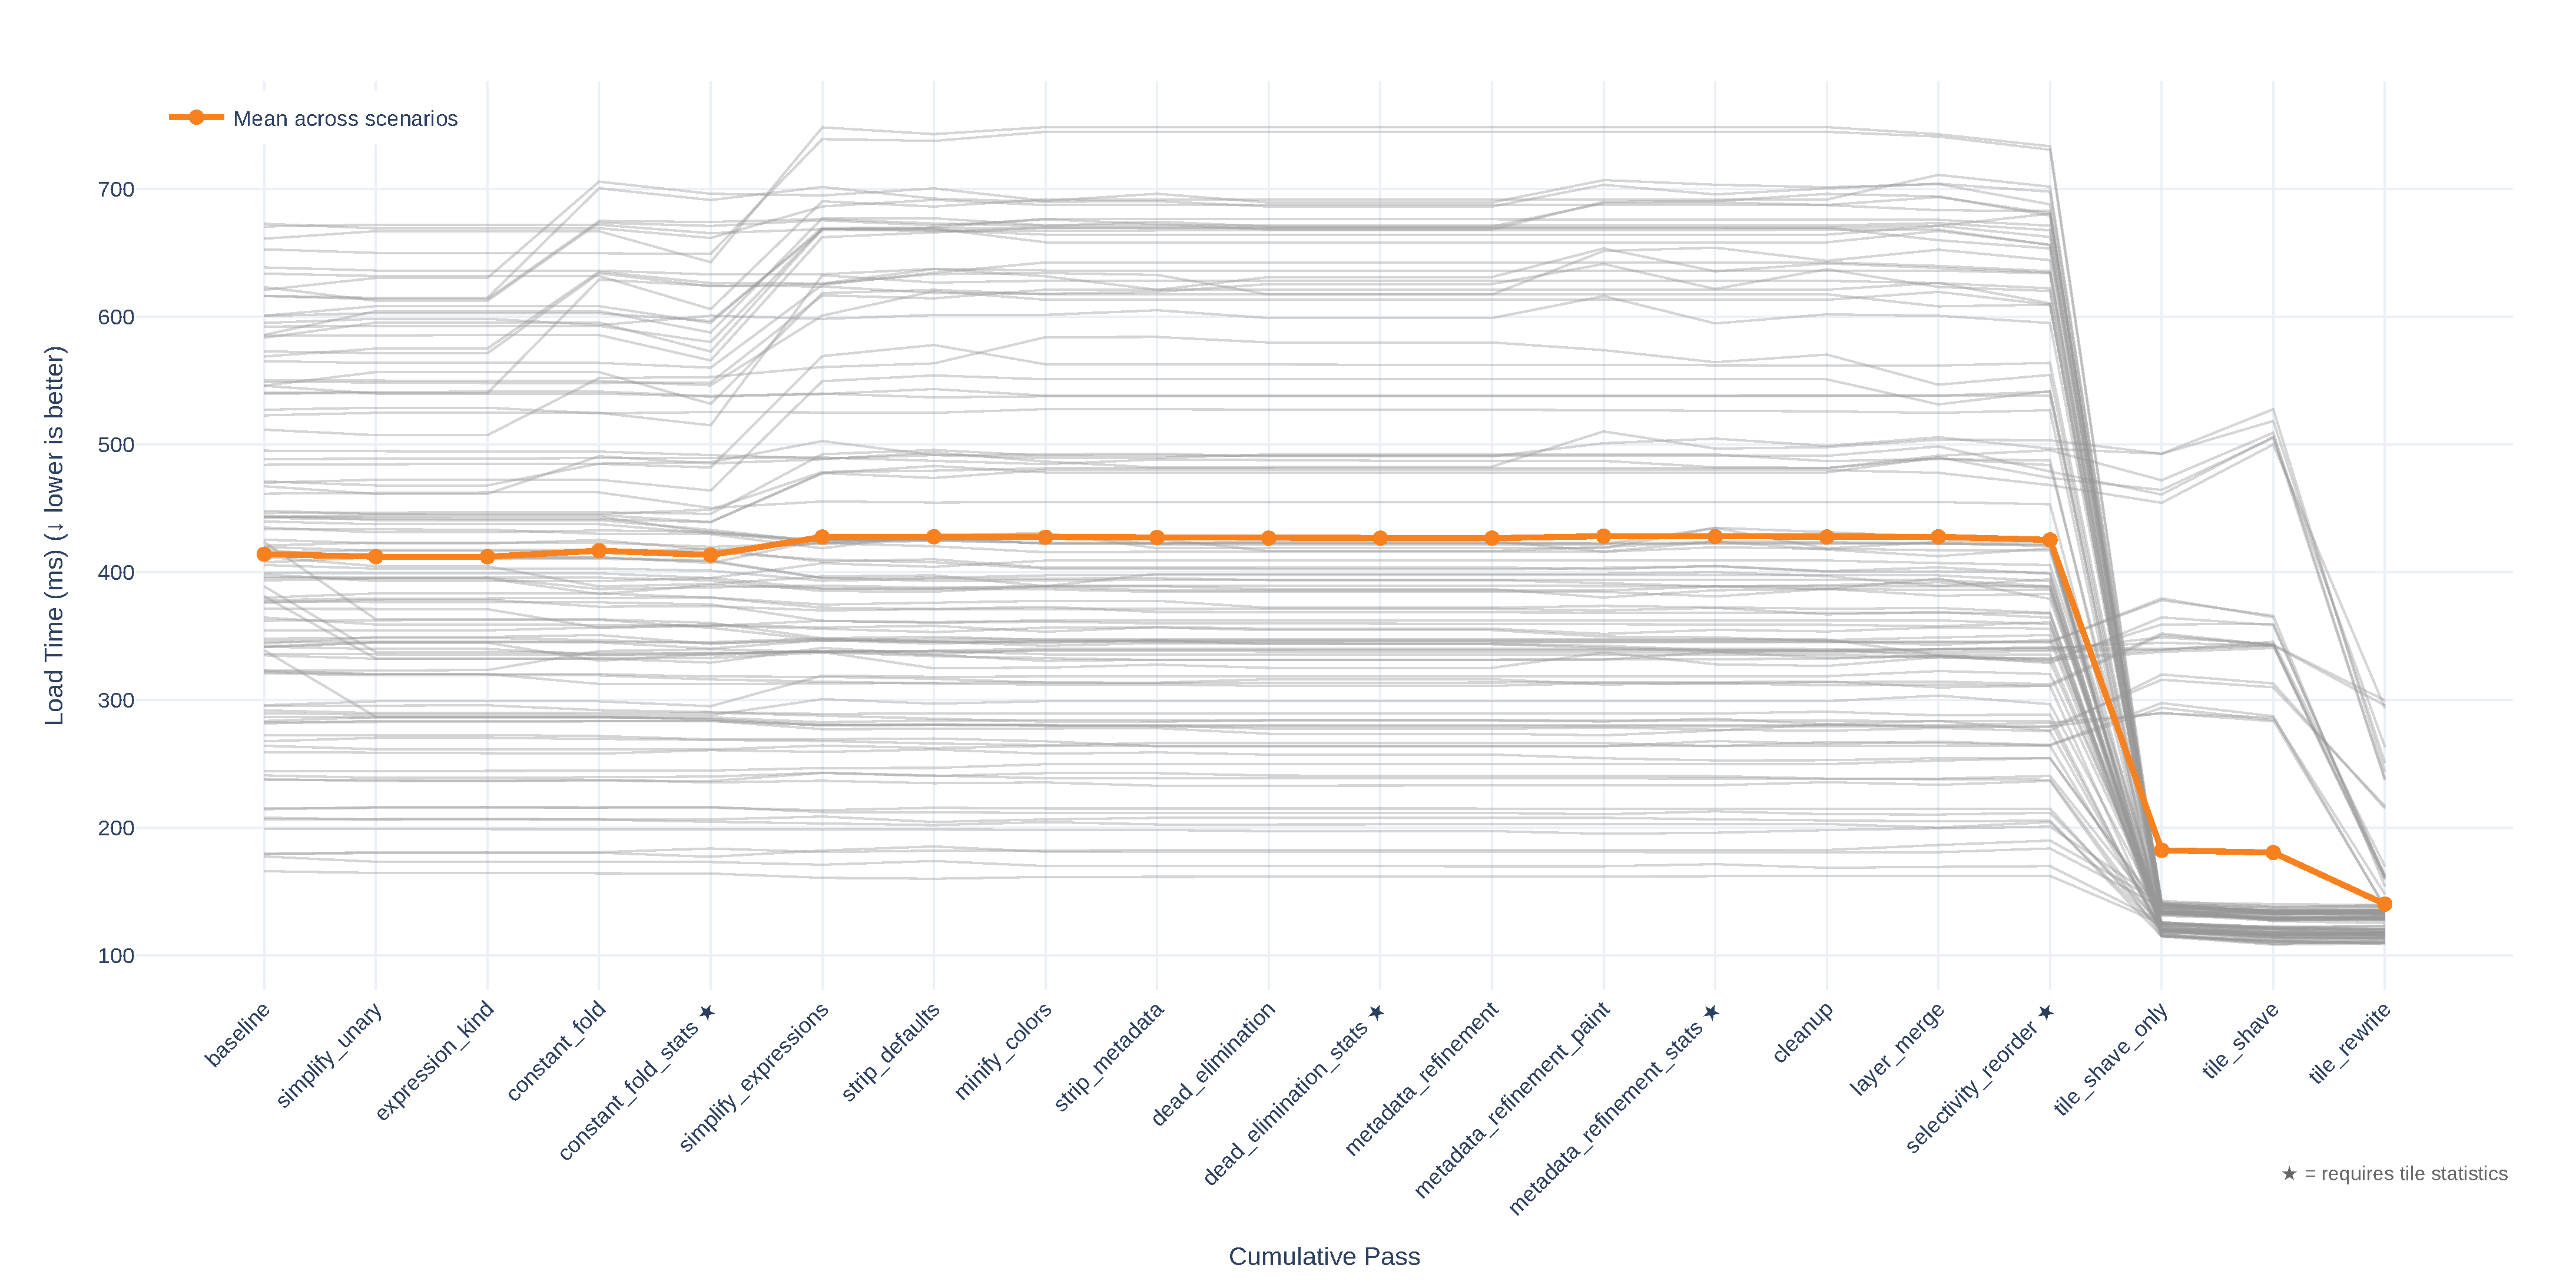
\includegraphics[width=\linewidth]{figures/waterfall_loadMs.pdf}
    \caption{Cumulative ablation waterfall for load time. Each bar shows the median change introduced by adding one expression pass on top of all previous passes, aggregated across all 18 scenarios and 15 benchmark styles. We can see that in the extremes, unary simplifcation has the largest effect; the aggregate load-time improvement across all expression passes is modest (\qty{-1.8}{\percent}), with expression passes serving primarily as enablers for downstream structural and data-level passes. For caveats, please see \cref{sub:expr_discussion}}
    \label{fig:waterfall_loadMs}
\end{figure}

\begin{figure}[htbp]
    \centering
    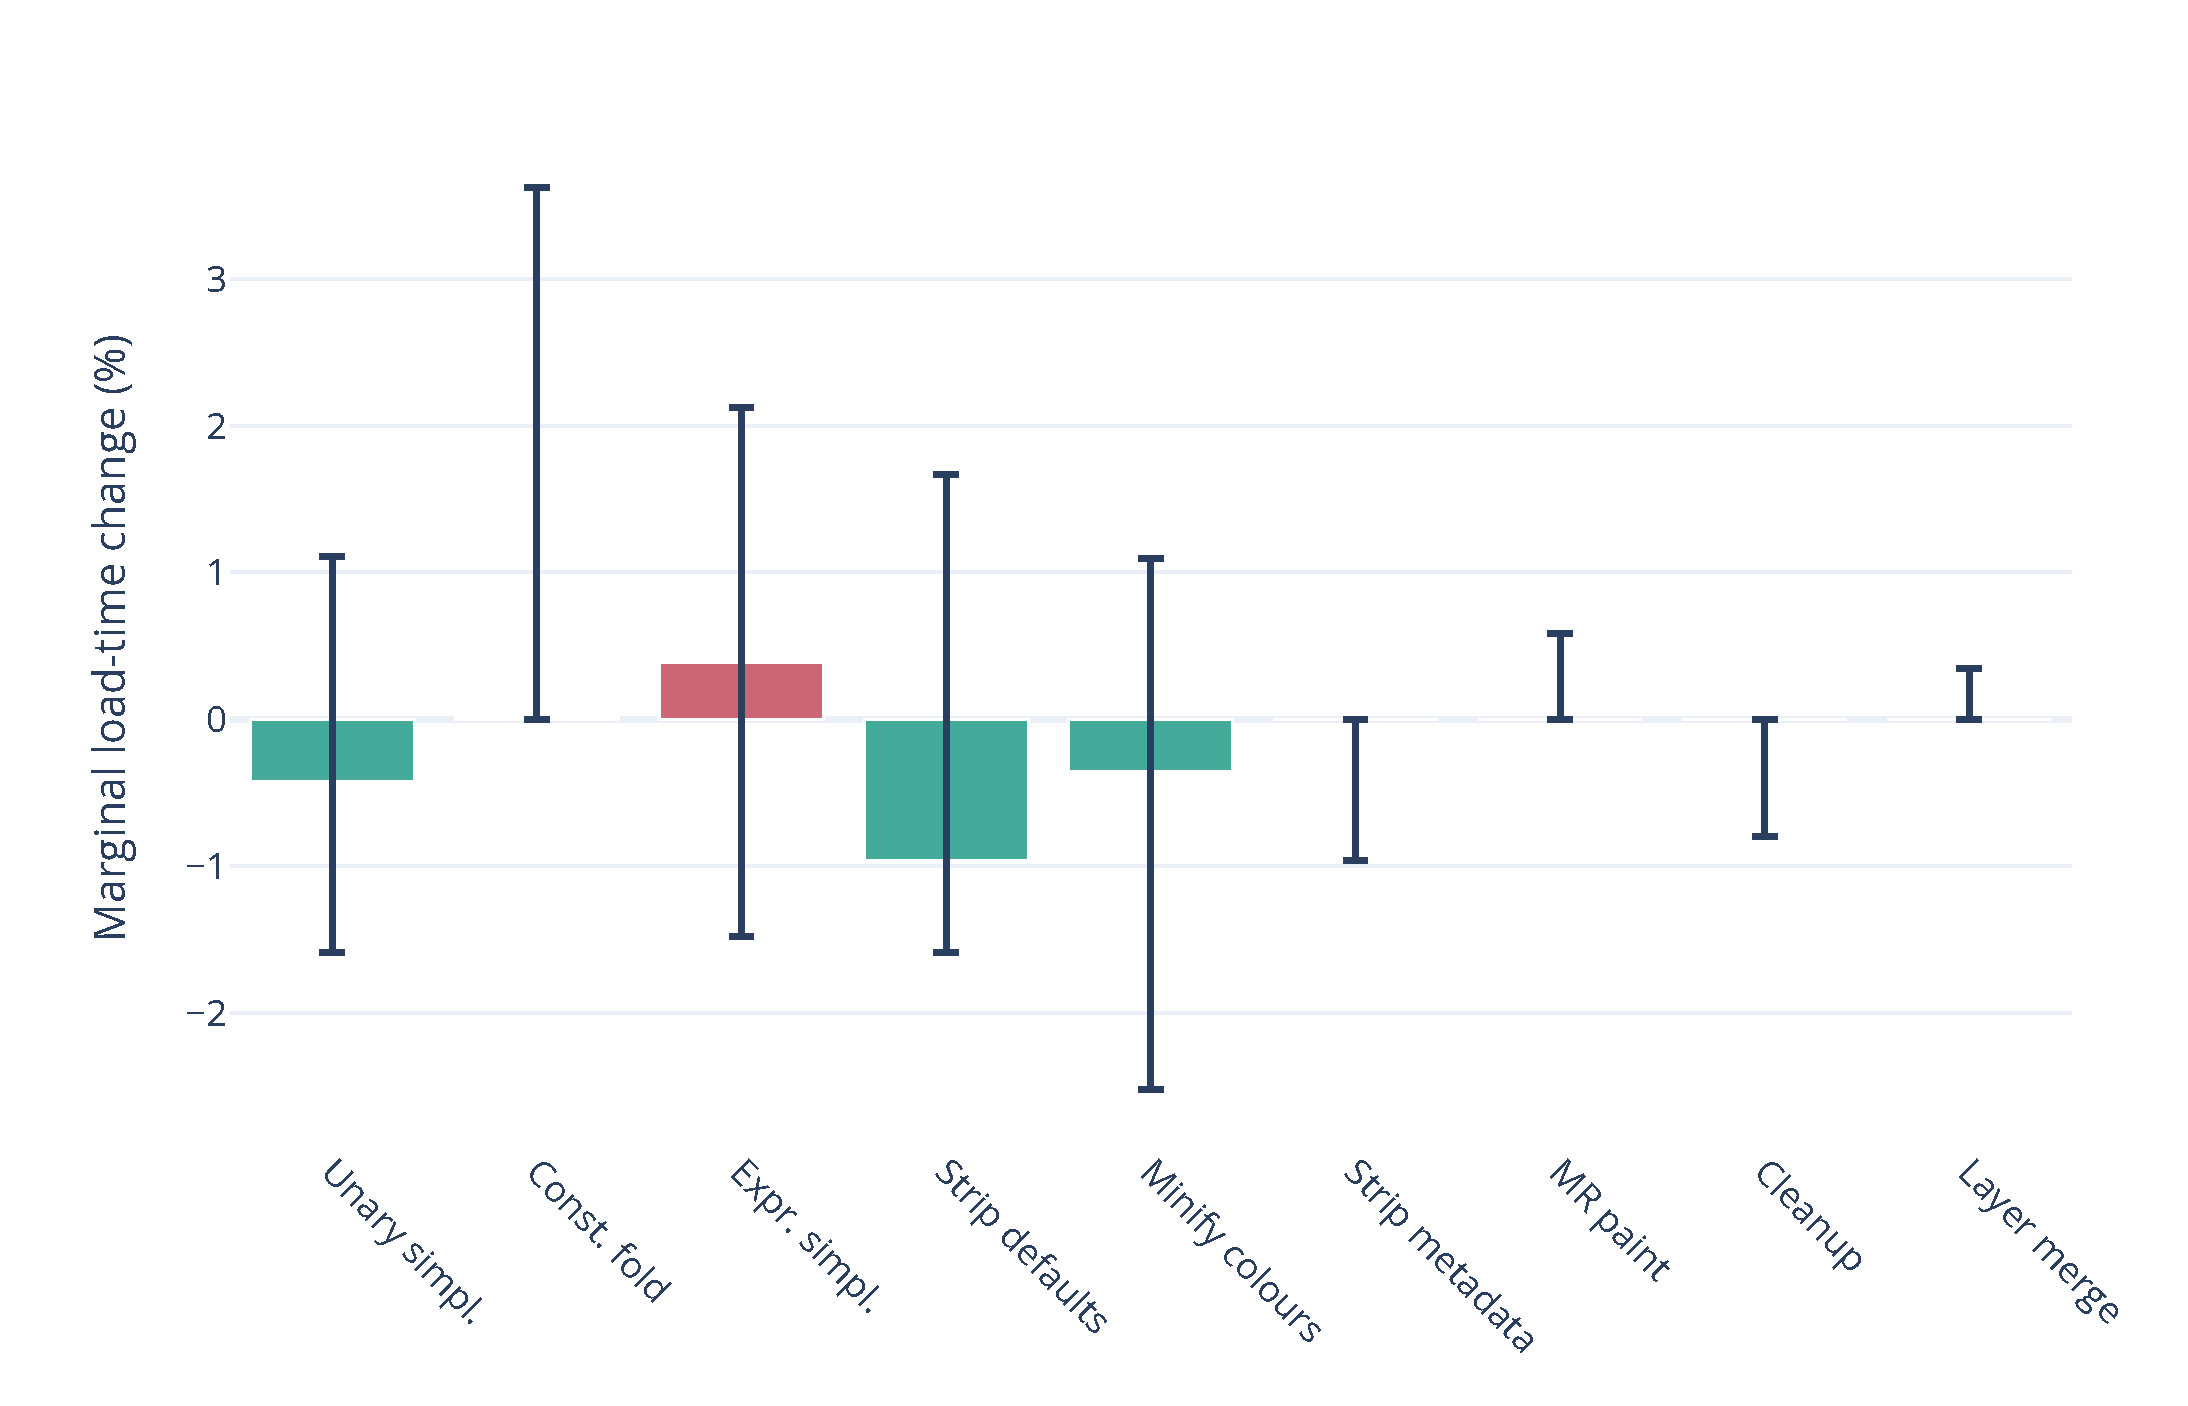
\includegraphics[width=\linewidth]{figures/marginal_loadMs.pdf}
    \caption{Marginal contribution of each expression pass to load time reduction shows the effect of each of the passes cleanly. }
    \label{fig:marginal_loadMs}
\end{figure}

\begin{figure}[htbp]
    \centering
    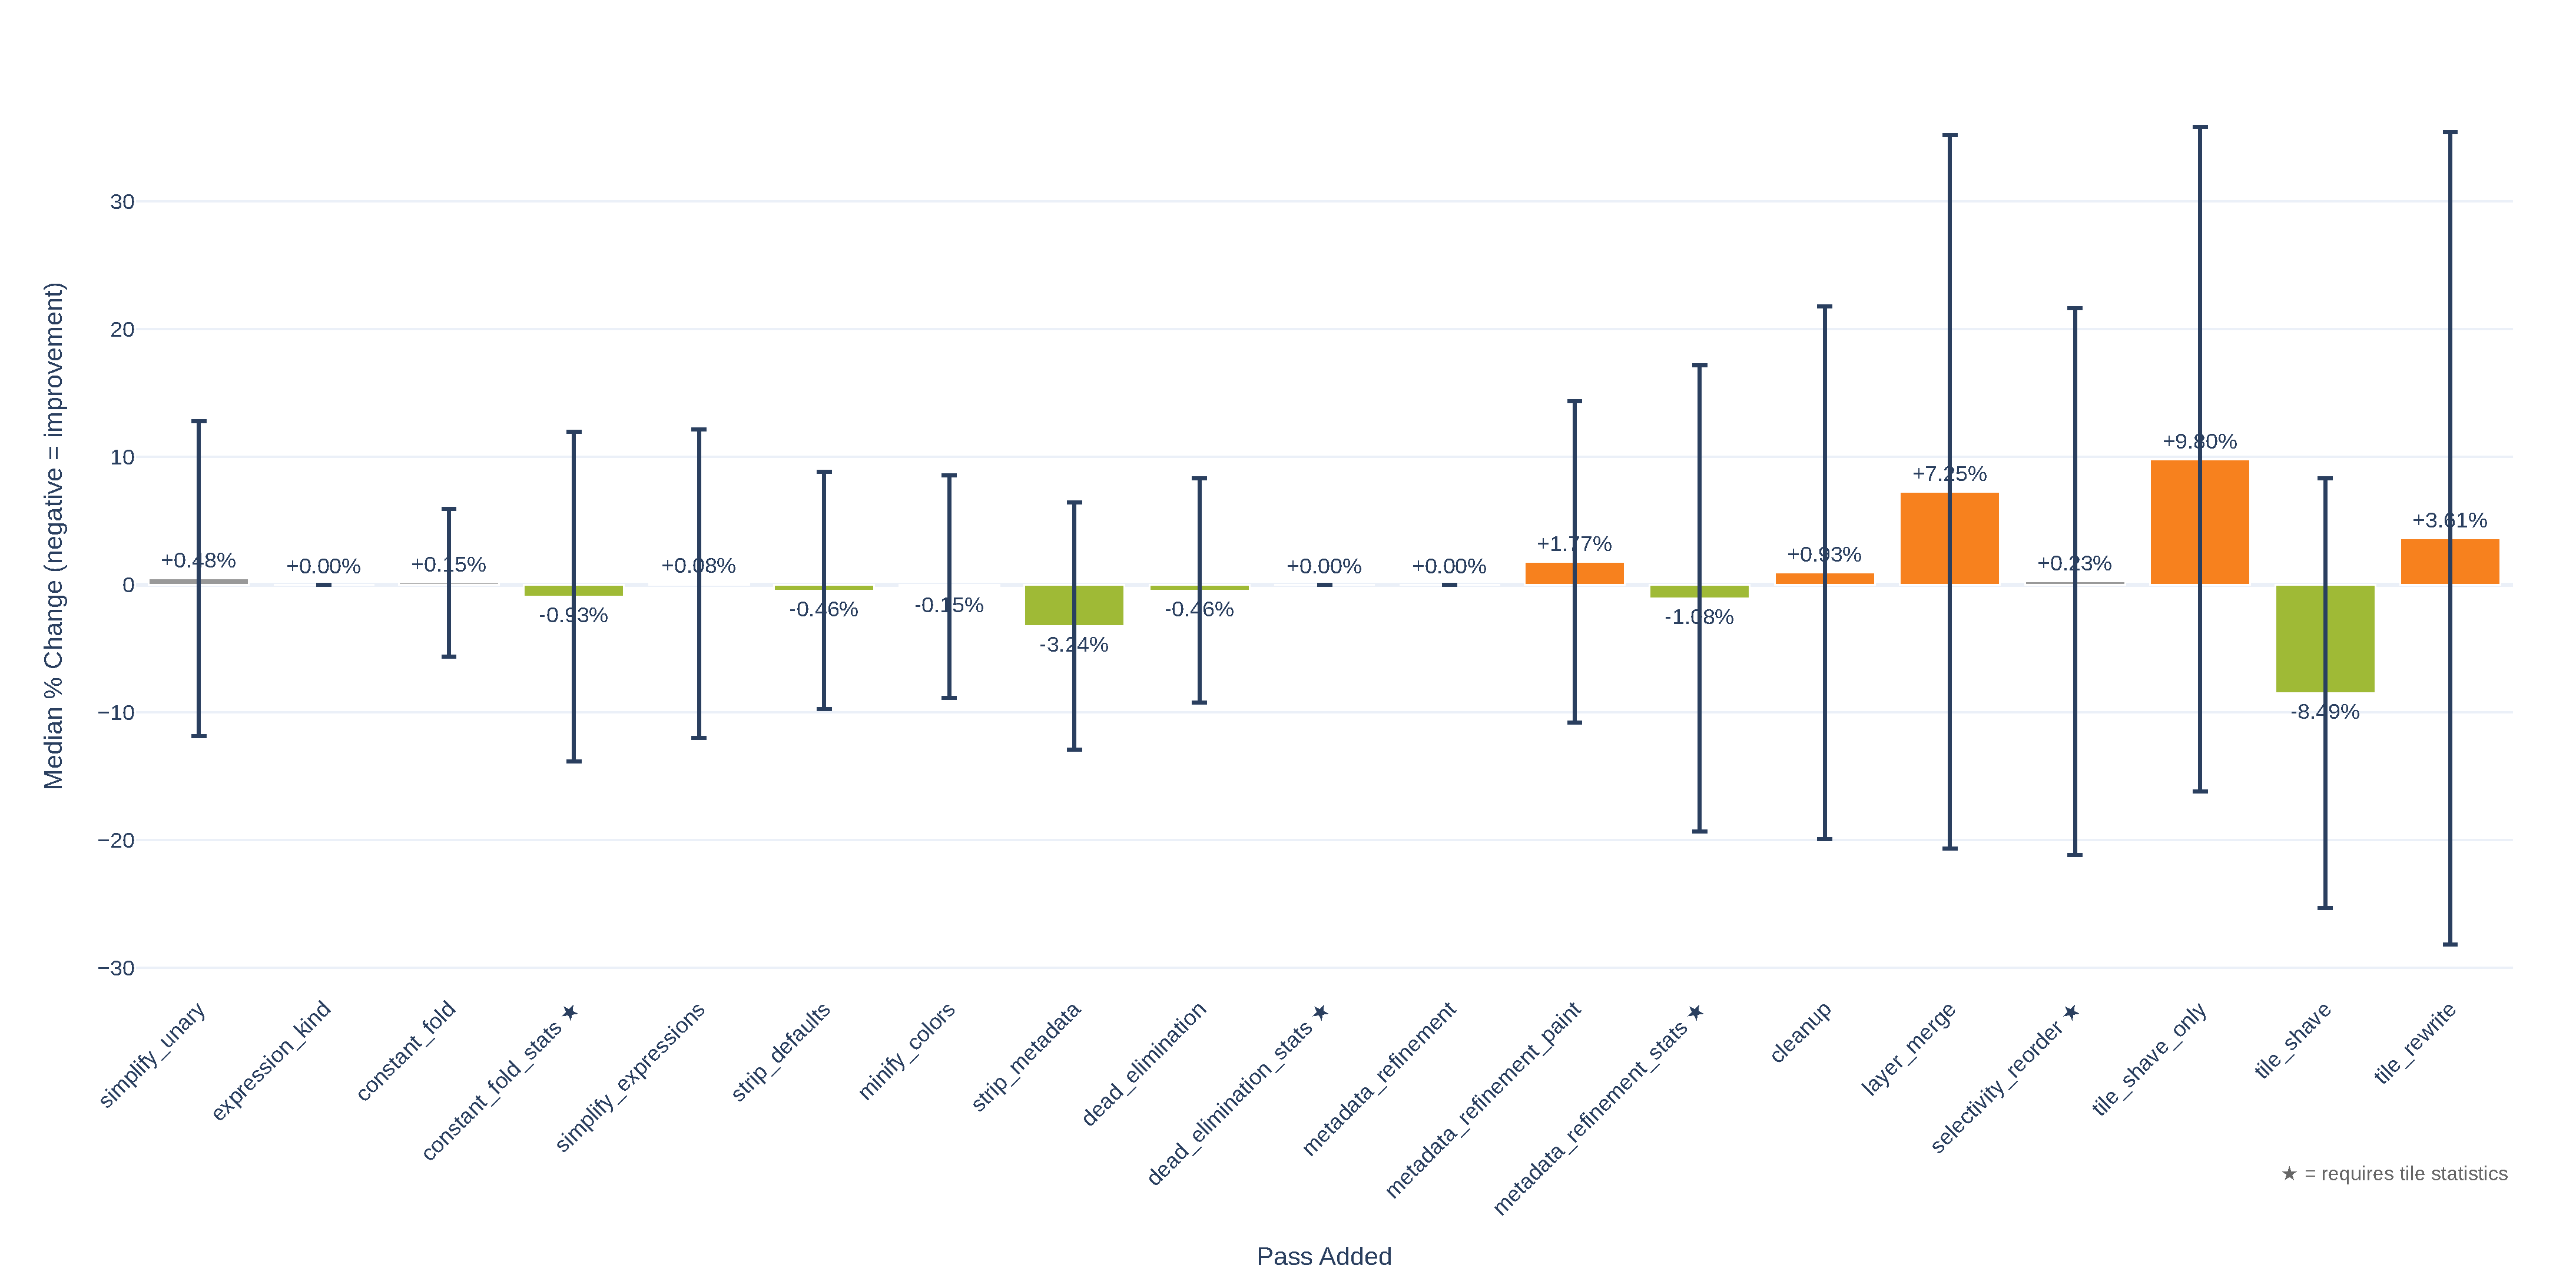
\includegraphics[width=\linewidth]{figures/marginal_styleParseMs.pdf}
    \caption{Marginal contribution of each expression pass to \texttt{styleParseMs}. The size-reducing passes (default stripping in particular) shorten the parse step monotonically, even where their end-to-end load-time effect is within noise; this is the proximate mechanism behind the style-parse leg of the time breakdown in \cref{fig:time_breakdown}.}
    \label{fig:marginal_styleParseMs}
\end{figure}

\subsection{Discussion}\label{sub:expr_discussion}

Expression passes shave only \qty{1.8}{\percent} from median load time, but raw style size drops by up to \qty{20.3}{\percent} on Fiord, with most of the size win concentrated in a single pass (default stripping).
We use the rest of this section to explain why one outlier pass dominates the per-style picture and why the size-reduction story diverges from the rendering-time one.

\paragraph{Unary simplification dominates}
Some styles are implemented in a not optimal way and thus allow a very high unary simplification gain.
The gain of this simplification is non-representative and biases the results to look better than they are overall.
Only two of the style familys gain significant speedups, both of the times through what we think are typos in how the style is written.

We expect this: reducing an expression tree to a literal eliminates all per-feature evaluation cost for that expression, whereas algebraic simplifications merely shorten the evaluation path.
For some styles this does not hold and unary simplification is more effective due to expensive string index handling being collapsed into senatically identical, but faster variants.
Fixpoint iteration amplifies the effect: a single successful simplfication can cascade through nested expressions, collapsing entire subtrees in subsequent iterations.

\paragraph{Size reduction vs.\ rendering improvement}
Passes that primarily reduce serialized style size - default stripping, color minification - show smaller rendering improvements but contribute meaningfully to transfer size under compression.
This primarily benefits time to first render (discussed in \cref{sub:combined_marginal}).
We note the distinction between raw, gzip, and Brotli reductions: some rewrites (e.g., \mlop{\texttt{any}}$\to$\mlop{\texttt{in}}) increase raw token count while decreasing compressed size, because the repetitive structure of \mlop{\texttt{in}} operand lists compresses well.

\paragraph{Selectivity reordering is empirically unmeasured}
Selectivity reordering (step~16) is a theoretically motivated heuristic whose isolated rendering impact we did not measure in this evaluation.
Because it appears late in the cumulative ablation, its marginal contribution is confounded with the preceding passes.
We acknowledge the independence assumption underlying the selectivity estimates as inaccurate for correlated map predicates (\cref{sec:query_optimizations}), and the empirical benefit may be negligible for styles whose filters are already short.

\paragraph{Downstream interaction with the data pipeline}
Beyond their direct rendering benefit, expression-level simplifications feed into the data-level pipeline evaluated in \cref{sec:exp_mlt}.
Each folded filter predicate and each pruned \mlop{\texttt{match}} arm reduces the set of property names and categorical values that the tile pruning advisory (\cref{sub:tile_shaving}) must track; each filter reduced to \mlval{\texttt{false}} enables dead layer elimination in the structural phase, which removes that layer's entire property footprint from the advisory.
Simpler filters are also more amenable to the advisory's static analysis, because canonical forms (e.g., a direct \texttt{[\mlop{"=="},~\ldots]} rather than a double-negated comparison) expose referenced property values more readily.
The magnitude of this interaction is quantified in \cref{sec:exp_mlt}.


\section{Experiment 2: Structural Optimizations}\label{sec:exp_structural}
\begin{keytakeaways}
\item Dead-layer elimination and layer merging produce nearly all the structural-family gains;\newline
      the other passes are negligible on their own.
\item Layer merging can grow raw bytes yet still shrink frame time - gzip absorbs the difference.
\item Symbol-heavy styles benefit less because symbol layers are excluded from merging.
\end{keytakeaways}

\noindent Where the previous experiment rewrote local expressions, in this one we evaluate the passes that reason across layers and sources - the structural family of \cref{sub:structural_optimizations}.

\subsection{Pass Interactions}\label{sub:structural_interactions}

Several pairwise dependencies between structural passes shape what we measure in the cumulative ablation in \cref{sub:structural_results}.
Expression passes must run first so that metadata refinement sees zoom predicates in their canonical form; dead elimination must precede layer merging because a dead layer between two otherwise-mergeable live layers blocks the merge.
Similarly, metadata refinement must precede cleanup so the residual \mlval{\texttt{true}} filters and zero-opacity layers it produces can be removed.
We give the full ordering rationale in \cref{sub:pipeline}; the practical consequence here is that the marginal contribution of each later pass in the ablation will reflect work that an earlier pass enabled, not just the pass itself.

\subsection{Evaluation}\label{sub:structural_evaluation}

Structural passes correspond to ablation steps~8-15 within the cumulative ablation of \cref{sub:ablation}.
In addition to the rendering metrics from Experiment~1 (\cref{sub:metrics}), we report complexity metrics for the structural evaluation: layer count, filter count, and total expression node count.
We report the effects on performance generalized in \cref{sub:cross_results} (over the generalization corpus of \cref{sub:generalization_corpus}) and the effect of the expression-level steps this work builds upon in \cref{sec:exp_expressions}.

\subsection{Results}\label{sub:structural_results}

\cref{fig:complexity_layer_count} tracks layer count across the structural ablation steps, showing which passes concretely remove layers rather than merely rewriting them.
\cref{fig:complexity_total_expression_nodes,fig:complexity_filter_count} extend the complexity view to the two remaining metrics introduced in \cref{sub:structural_evaluation}: total expression-tree node count and filter count.
\cref{fig:style_size_ablation} complements these with the raw, gzip, and Brotli style sizes, confirming that the structural reductions also translate into smaller transfer size rather than just reshuffling the serialized form.


\begin{figure}[htbp]
	\centering
	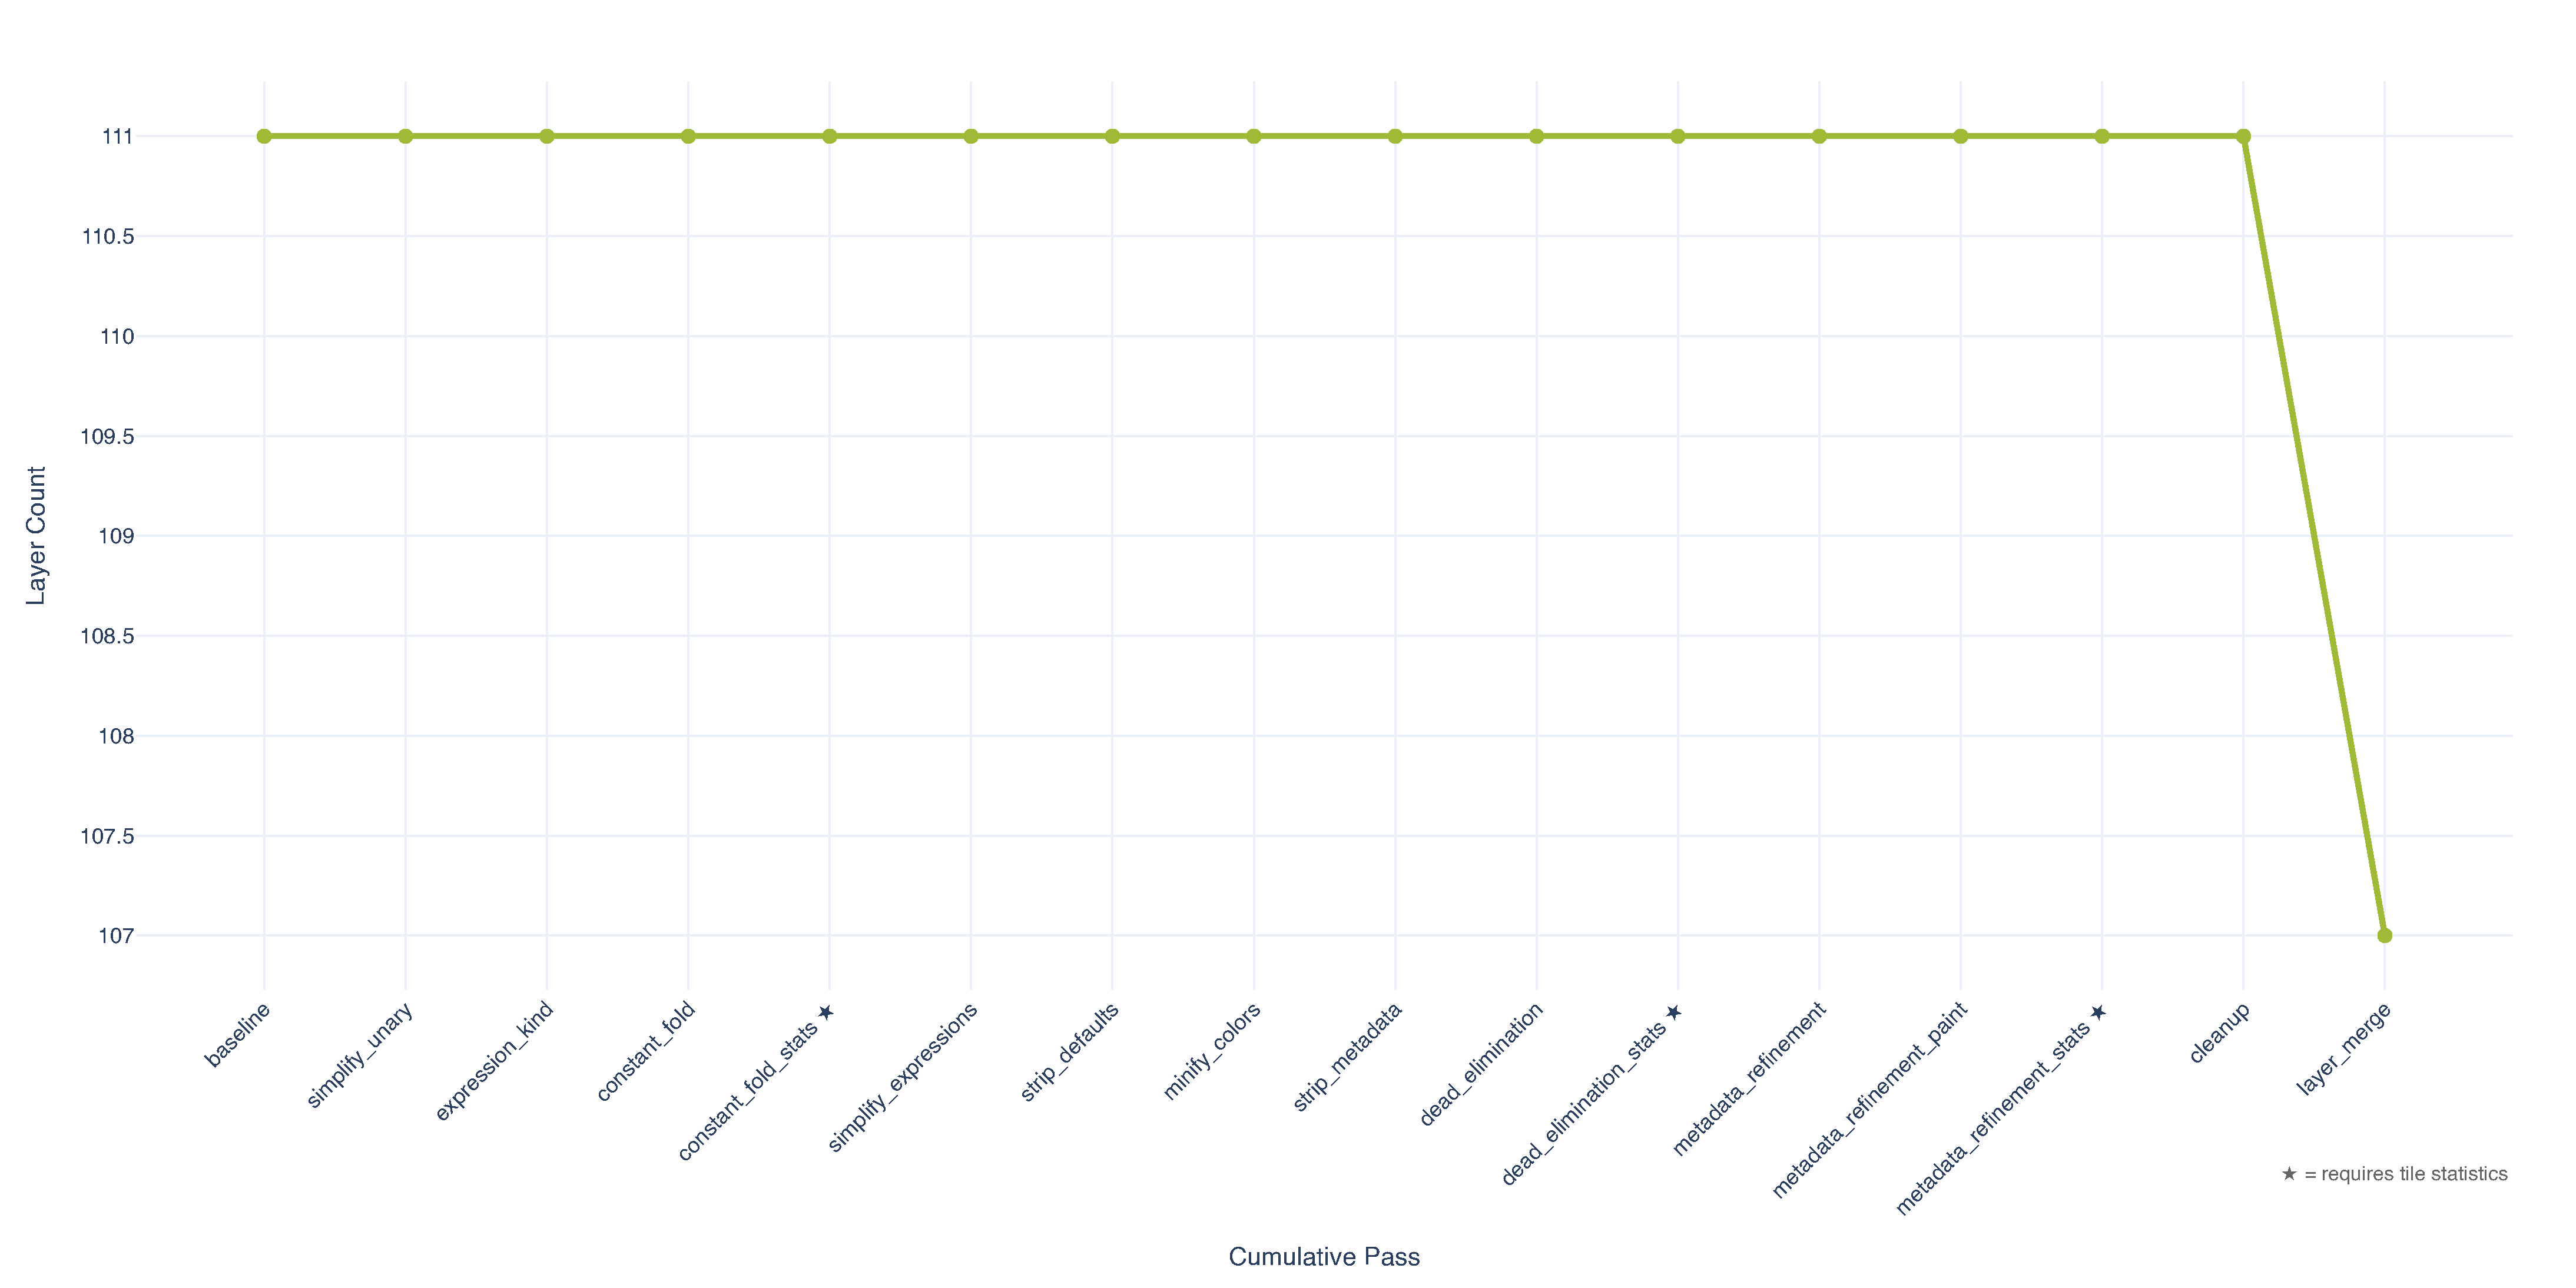
\includegraphics[width=\linewidth]{figures/complexity_layer_count.pdf}
	\caption{Layer count across cumulative ablation steps on the liberty style: only layer merging reduces the layer count. Dead elimination rarely removes whole layers, because styles are designed to expose parts of the map rather than leave entire layers unreferenced.}
	\label{fig:complexity_layer_count}
\end{figure}

\begin{figure}[htbp]
	\centering
	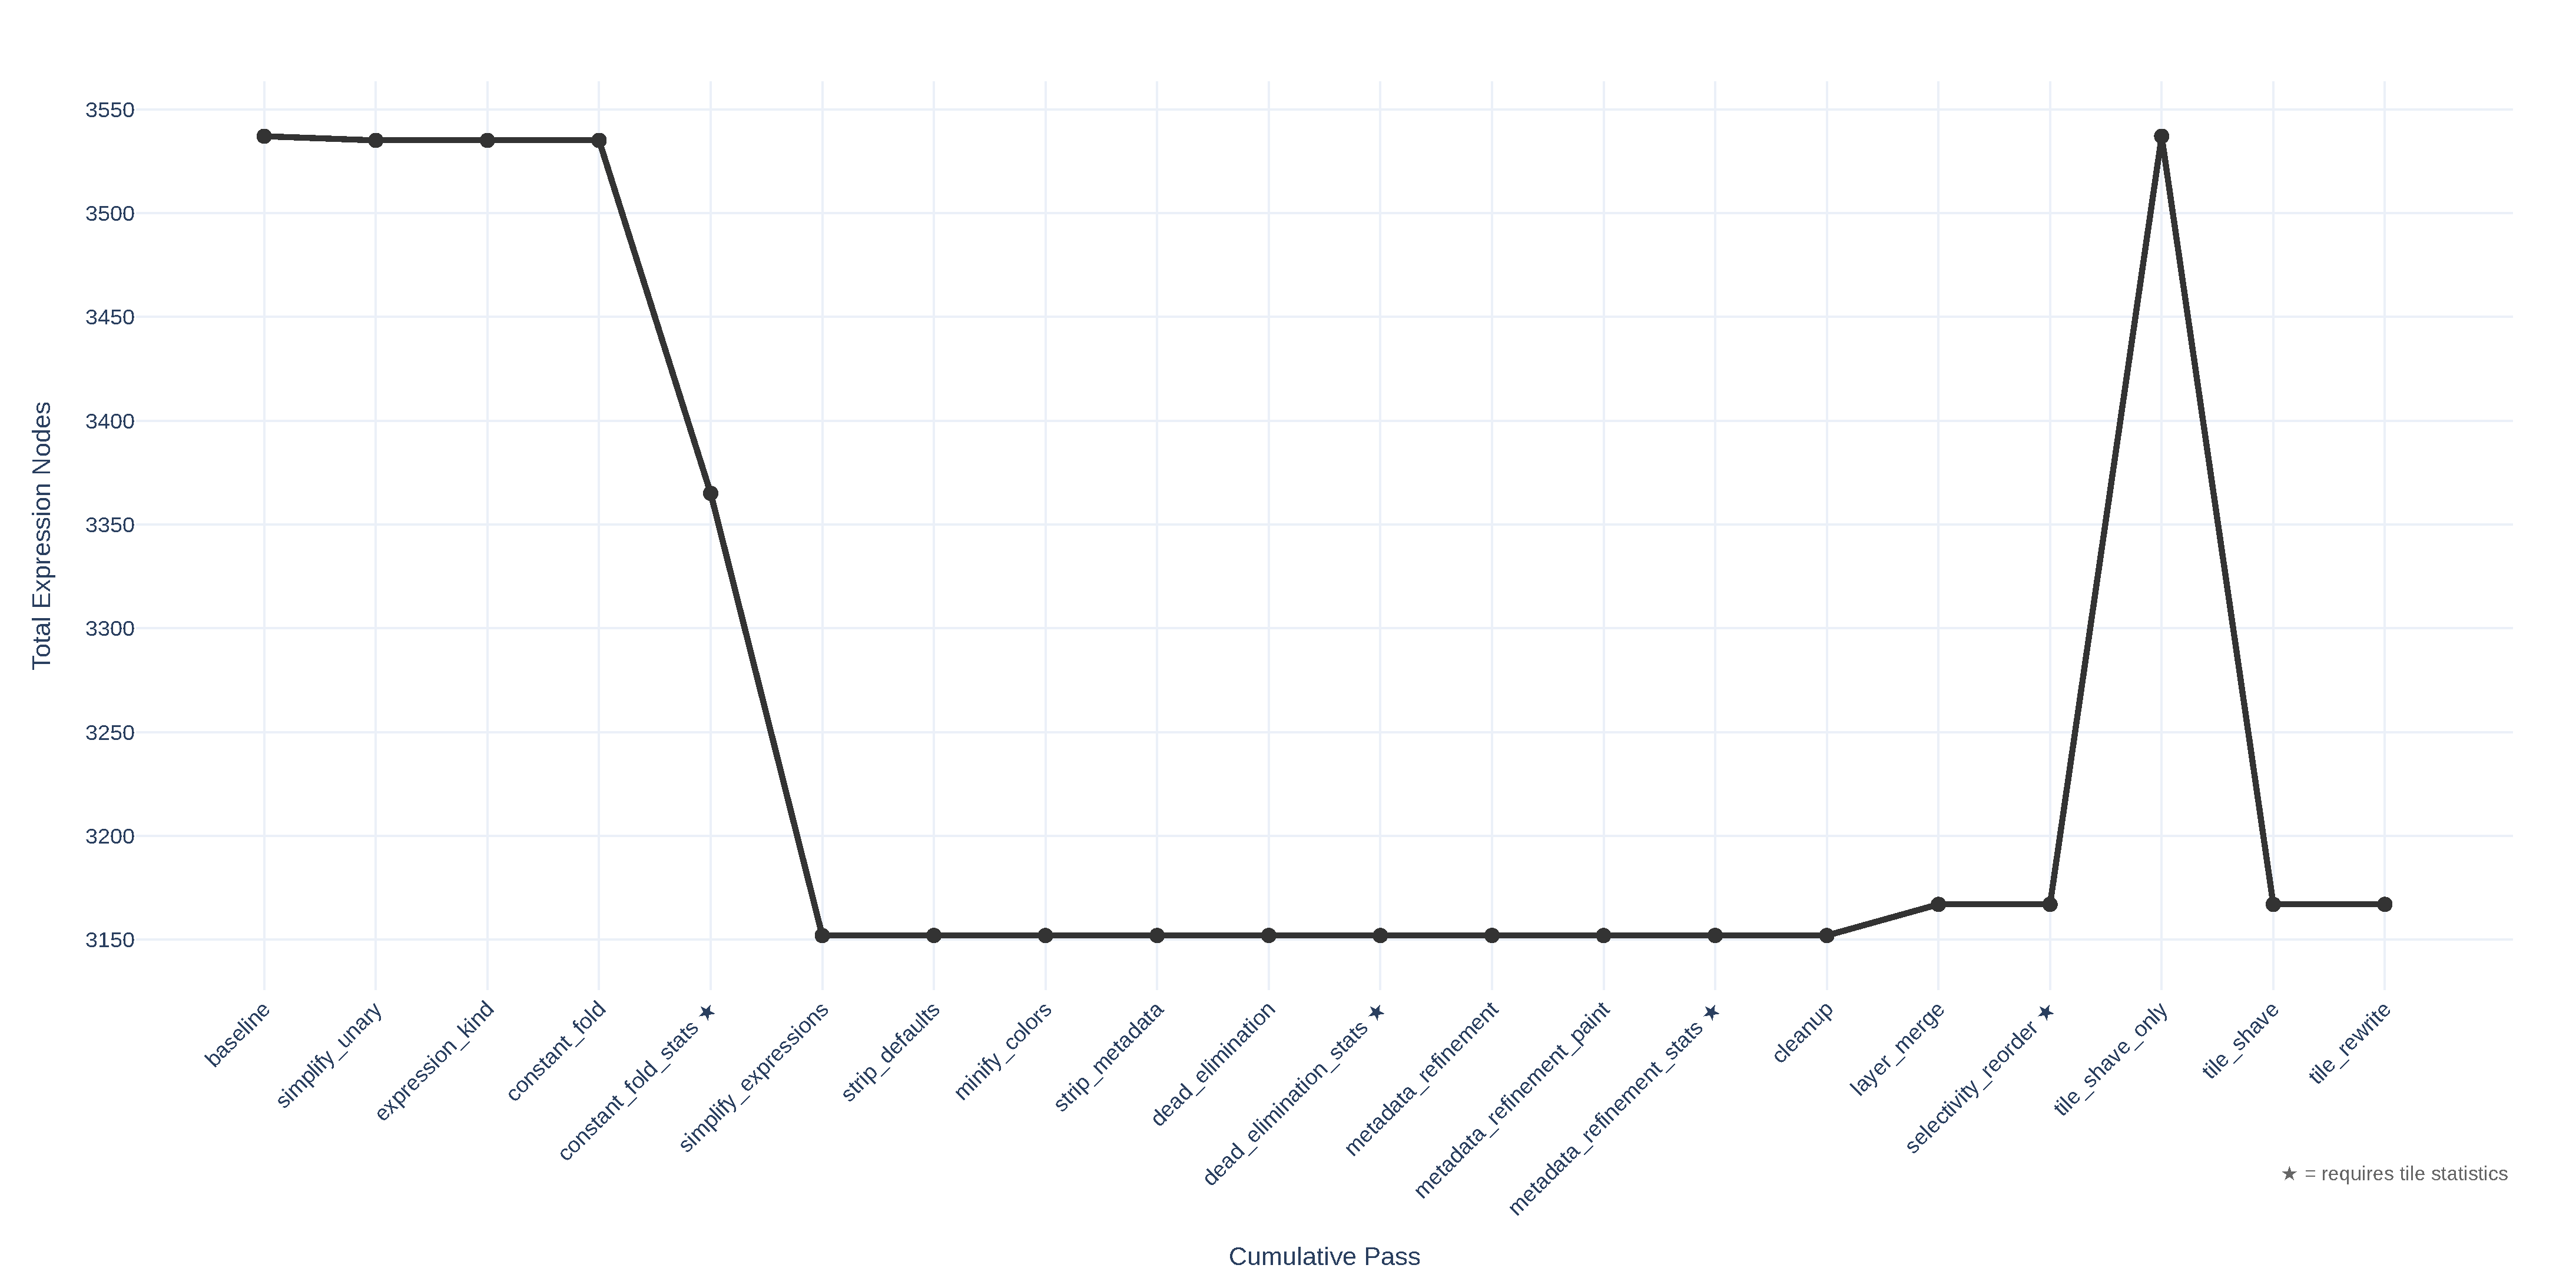
\includegraphics[width=\linewidth]{figures/complexity_total_expression_nodes.pdf}
	\caption{Total expression-tree node count across cumulative ablation steps. Expression passes (steps~1-7) produce the largest reductions, with Fiord dropping by \qty{36.8}{\percent} (\num{1610}$\to$\num{1018}) and Liberty by \qty{10.5}{\percent} (\num{3537}$\to$\num{3167}); structural passes contribute additional, smaller reductions by removing or merging layers that own subtrees.}
	\label{fig:complexity_total_expression_nodes}
\end{figure}

\begin{figure}[htbp]
	\centering
	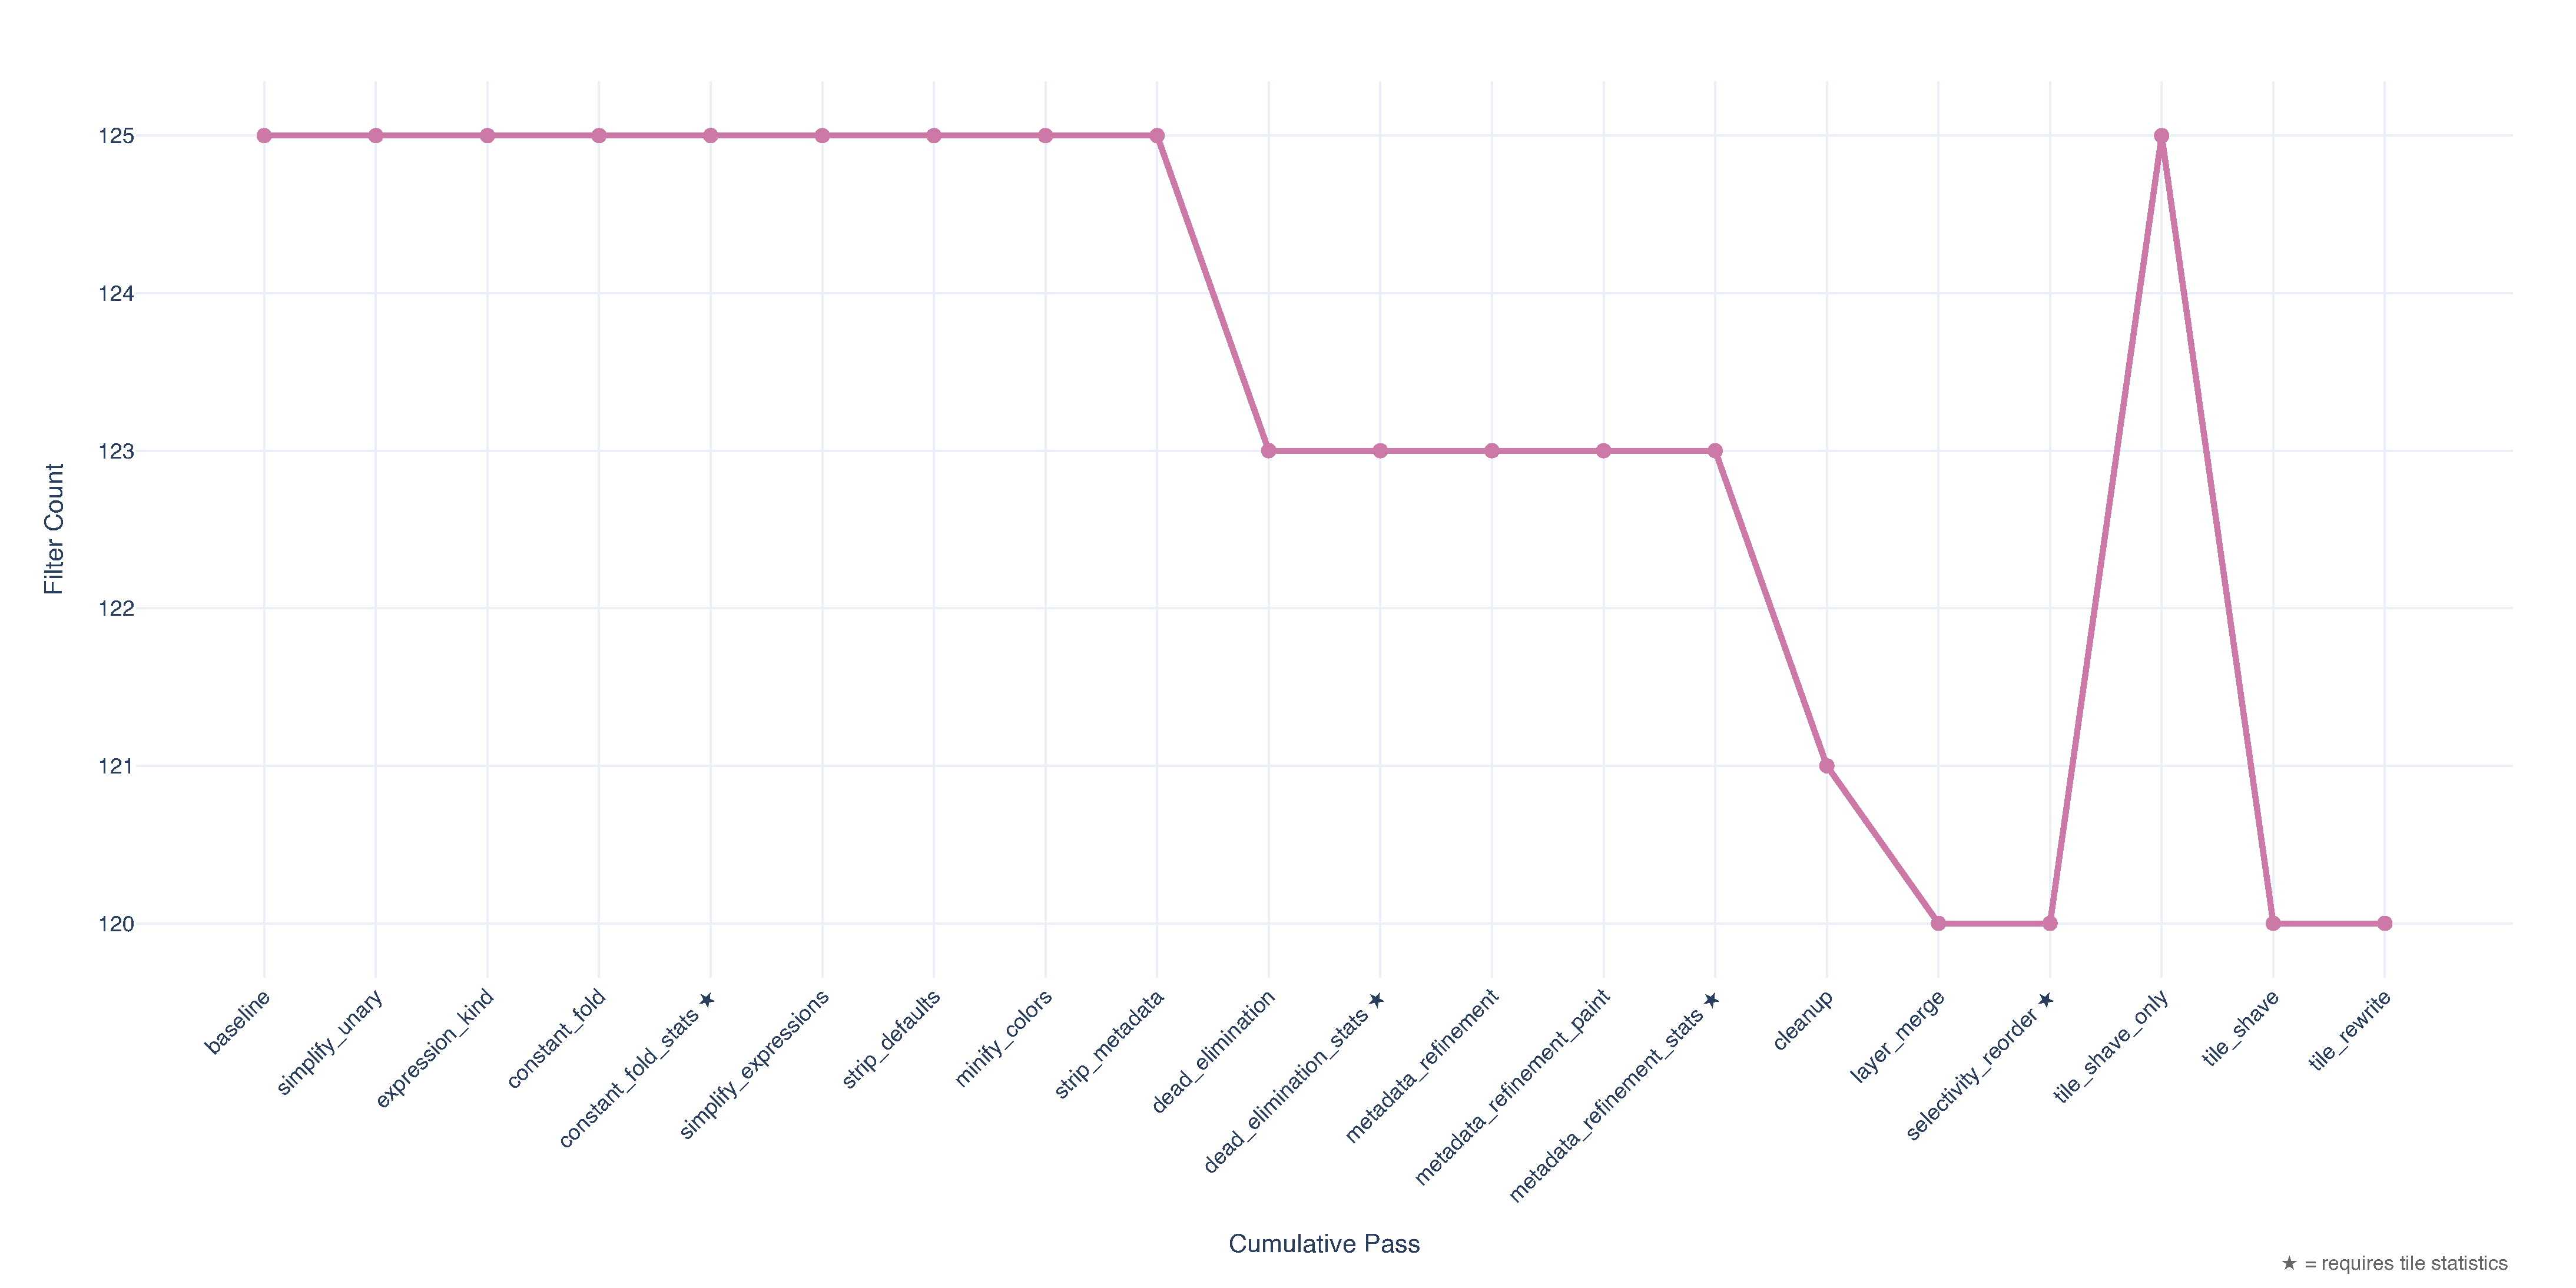
\includegraphics[width=\linewidth]{figures/complexity_filter_count.pdf}
	\caption{Filter count across cumulative ablation steps. Metadata refinement (consuming zoom predicates) and dead elimination drive most of the filter-count reduction; cleanup removes the residual \mlval{\texttt{true}} filters that refinement leaves behind.}
	\label{fig:complexity_filter_count}
\end{figure}

\begin{figure}[htbp]
	\centering
	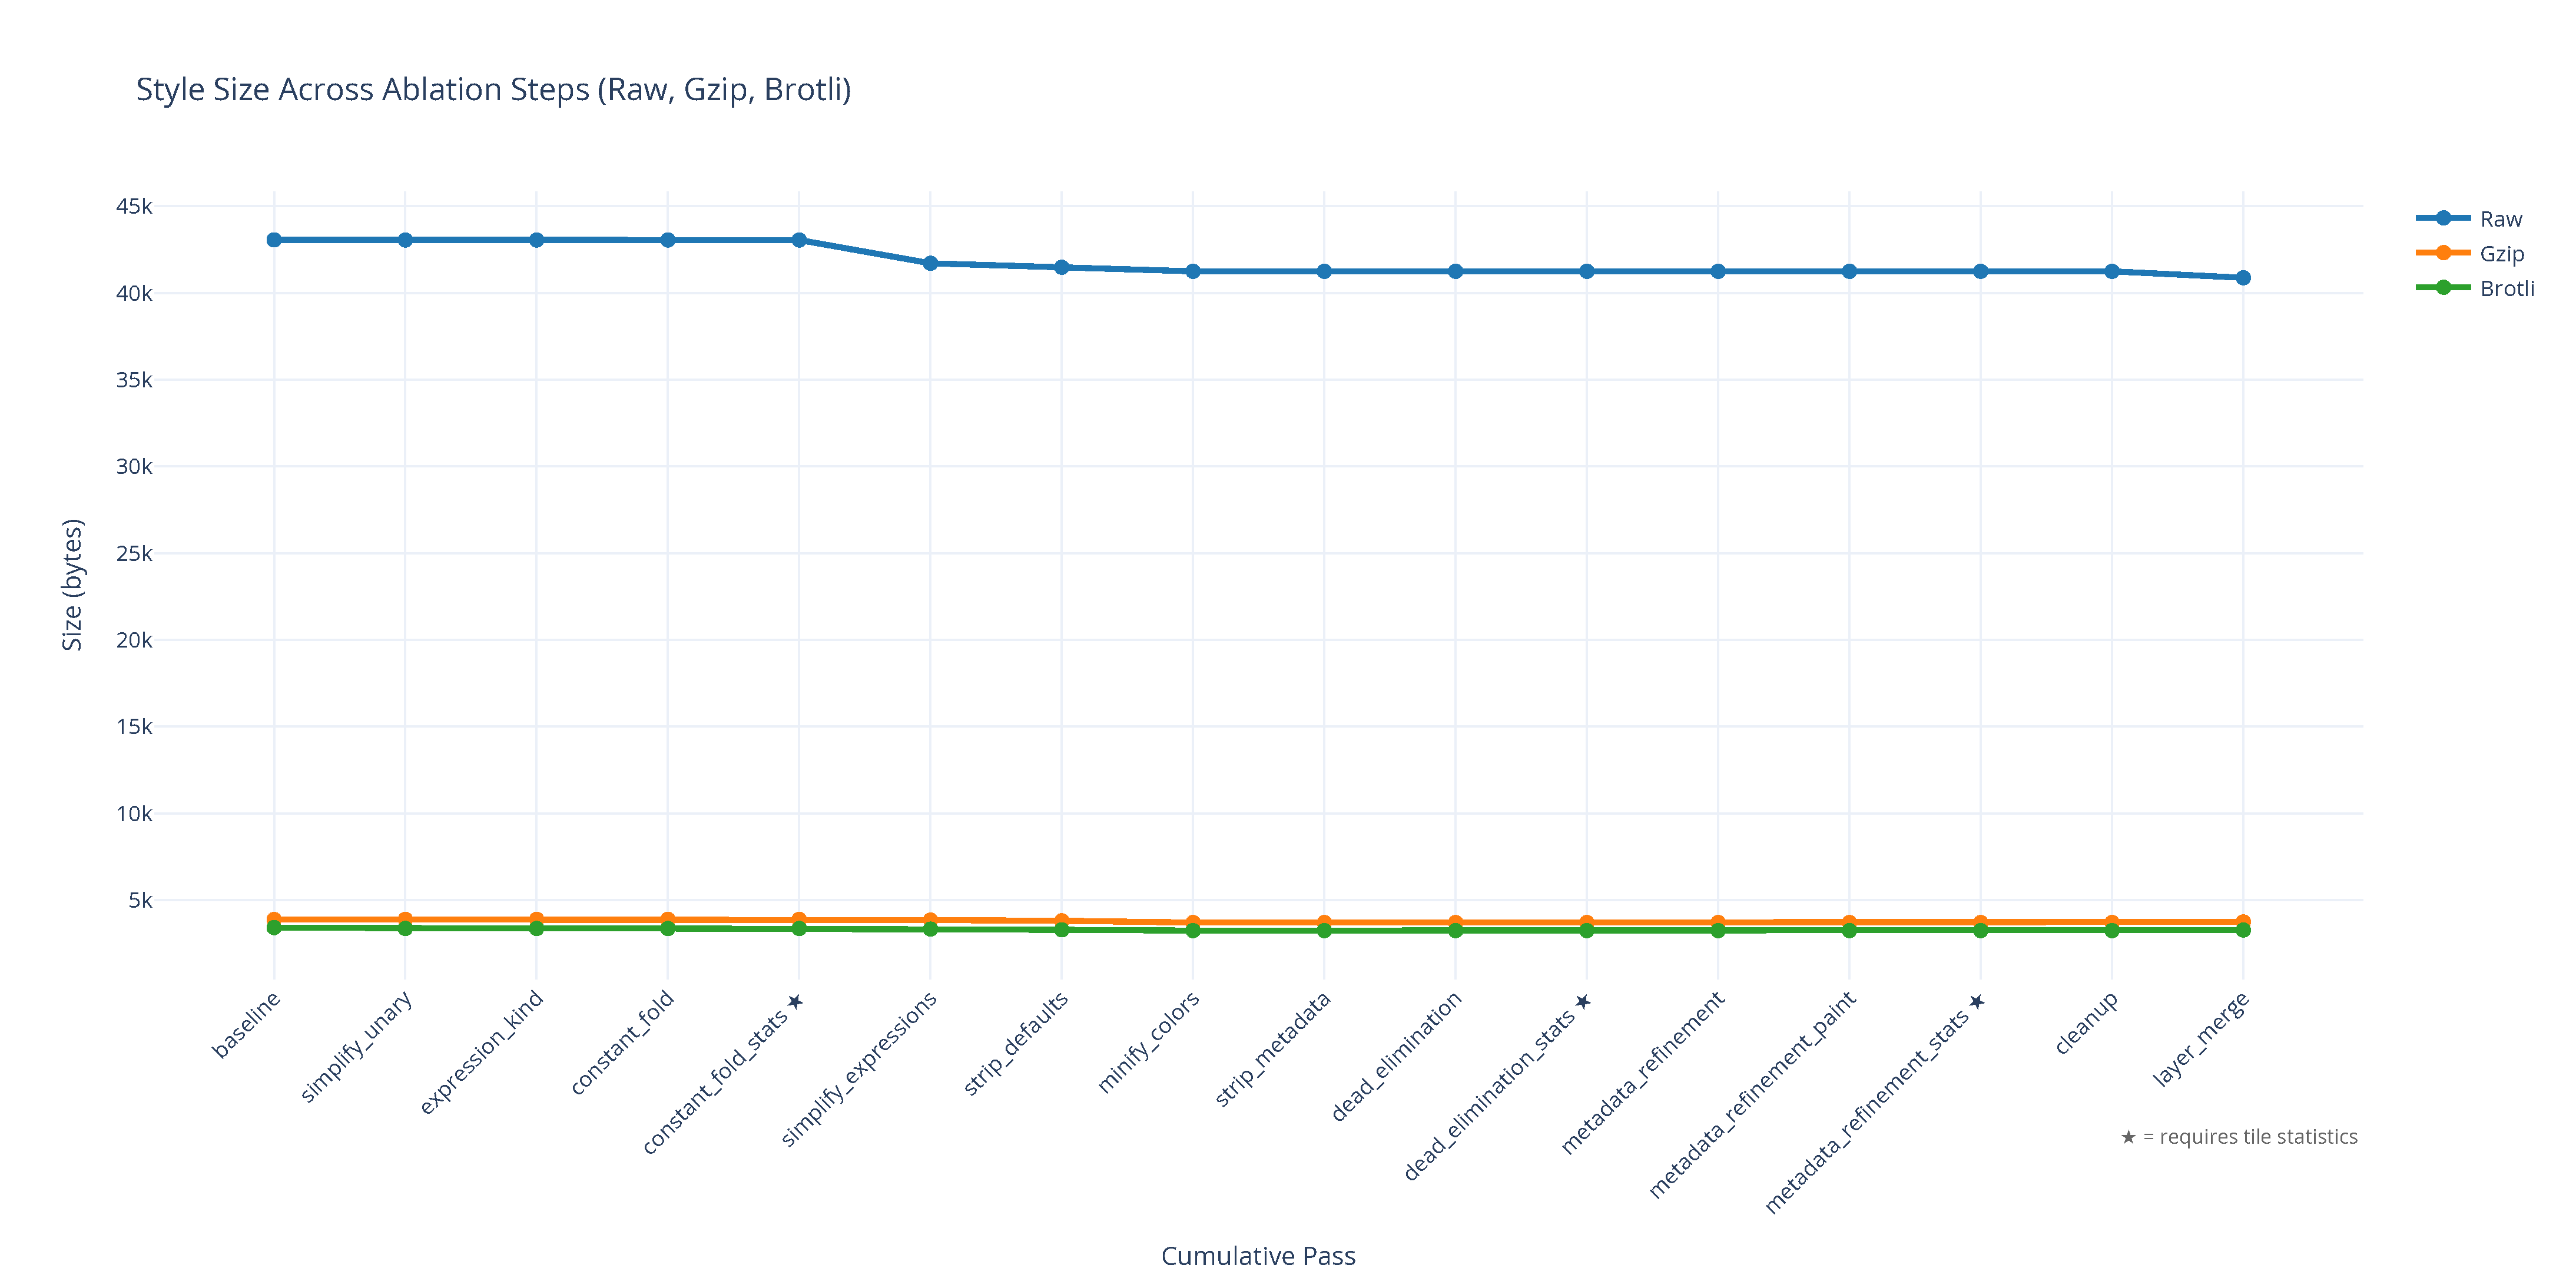
\includegraphics[width=\linewidth]{figures/style_size_ablation.pdf}
	\caption{Style size (raw, gzip, Brotli) across ablation steps: the effect on this metric is incremental rather than transformative.}
	\label{fig:style_size_ablation}
\end{figure}

The magnitude of structural improvement is style-dependent.
Fiord's layer count drops from 48 to 46 (\qty{-4.2}{\percent}), with dead elimination removing one layer (step~9) and cleanup removing another (step~14) after metadata refinement lifts zoom predicates that leave a filter as \mlval{\texttt{true}} on an invisible layer.
Liberty's layer count drops from 111 to 107 (\qty{-3.6}{\percent}), concentrated entirely in the layer-merge step (step~15), which merges four pairs of adjacent layers with compatible filters.
In terms of gzip transfer size, Fiord benefits substantially (\qty{-14.1}{\percent} from baseline to step~15), while Liberty sees a modest \qty{-4.9}{\percent}, with layer merging slightly \emph{increasing} gzip by \qty{36}{\byte} due to the larger merged filter expressions.
Expression-tree complexity tells a similar per-style story: Fiord's total expression-tree node count drops by \qty{36.8}{\percent} (\num{1610}$\to$\num{1018}), whereas Liberty's drops by \qty{10.5}{\percent} (\num{3537}$\to$\num{3167}).

\subsection{Discussion}\label{sub:structural_discussion}

Two of the six structural passes - dead-layer elimination and layer merging - produce nearly all of the gain, cutting Fiord's gzip transfer by \qty{14.1}{\percent} and Liberty's by \qty{4.9}{\percent}.
The following paragraphs unpack why those two dominate and how the remaining passes contribute indirectly or feed into the data-level pipeline downstream.

\paragraph{Dead elimination and layer merging dominate}
Among the structural passes, dead elimination and layer merging produce the largest improvements in both rendering performance and style complexity.
Dead elimination directly reduces the number of layers the renderer must process per frame; layer merging reduces draw calls by combining multiple rendering passes into one.
The interaction between the two is synergistic: styles with many narrowly-filtered layers (e.g., road styles that define separate layers for each road class) benefit most, as dead elimination first removes layers for road classes absent from the data, and layer merging then combines the remaining layers into a single multi-class layer.

\paragraph{Layer merging can trade raw size for runtime savings}
Layer merging does not always reduce the raw serialized byte count.
A merged layer replaces $k$ small filter expressions with a single \mlop{\texttt{match}}-keyed filter and $k$-armed \mlop{\texttt{match}} expressions for every differing paint property, which for small $k$ can produce a slightly larger textual representation than the sum of the originals.
The per-style ablation tables in \cref{sec:app_per_style} show one such case (Bright: \num{44.4}$\to$\qty{44.6}{\kilo\byte} after layer merging), where the raw count creeps up while the layer count drops by one (119$\to$118).
This was uncomfortable when we first saw it in the runs, since the intuition is that merging should shrink the style, but raw byte count turns out to be a proxy for parse time and transfer cost rather than for rendering cost, which is driven by layer count and per-frame draw calls.
The merged layer is still cheaper to render even when its serialized form is bigger, and the gzip and Brotli columns of the same table show the compressed size essentially unchanged, so the raw increase disappears under realistic wire compression anyway.

\paragraph{Metadata refinement has indirect effects}
Metadata refinement does not directly reduce the number of layers or the complexity of expressions; instead, it enables the renderer to skip layers at zoom levels where they are invisible.
The rendering improvement is therefore zoom-dependent: at overview zoom levels (where many layers are filtered out by tightened \texttt{minzoom}), the improvement is large; at street-level zoom (where most layers are active), the improvement is smaller.
Paint-based refinement captures a class of optimizations that are invisible to filter analysis - a layer whose opacity interpolates from~0 at zoom~12 is indistinguishable from a fully visible layer when examining only the filter.

\paragraph{Stats-driven passes amplify style-only passes}
The marginal contribution of stats-driven dead elimination (step~10) over non-stats dead elimination (step~9) quantifies the value of tile statistics for style optimizations.
Styles that use broad \texttt{source-layer} references benefit most, as statistics reveal which geometry types and property values actually exist.
For styles that already have precise filters (e.g., hand-tuned Americana), the marginal gain is smaller.

\paragraph{Symbol layer exclusion}
We exclude symbol layers from merging because MapLibre's collision detection operates per-layer (we give the soundness argument in \cref{sub:structural_optimizations}).
The headline merging numbers above are therefore reductions in the non-symbol pool only.
Because styles are usually dominated by labels, most see proportionally smaller layer-count gains.

\paragraph{Downstream interaction with tile shaving}
Dead layer elimination has a second-order effect beyond reducing per-frame draw calls:
each eliminated layer removes its property references from the tile pruning advisory computed in the data-level pipeline (\cref{sub:tile_shaving}).
If a removed layer was the sole consumer of a property column, that column is stripped from every tile at encoding time.
Similarly, metadata refinement's tightened zoom bounds cause the advisory to mark additional zoom levels as unused for a given source-layer, potentially eliminating entire tiles.
We characterize this interaction fully in \cref{sub:mlt_discussion} and quantify it in \cref{sub:mlt_results}; the aggregate data shows that the composition is additive rather than synergistic, but the advisory-narrowing effect is a necessary precondition for style-dependent tile shaving.


\section{Experiment 3: Data-Level Optimizations}\label{sec:exp_mlt}
\begin{keytakeaways}
\item Tile shaving dominates: \qty{-71.5}{\percent} median load; style passes contribute additively, not synergistically.
\item The \ac{MLT} format alone is not the win - \ac{MLT}-Java drifts above $1.0\times$ \ac{MVT} under gzip/Brotli;\newline
    the gain comes from the encoder's strategy competition and shared dictionary selection in our new encoder.
\end{keytakeaways}

\noindent In \cref{sec:exp_structural,sec:exp_expressions} we optimized the \emph{program} the renderer executes; in this experiment we ask whether we can optimize the \emph{data} it consumes using the same style information, and to what extent the two levels interact - the joint-optimization question at the heart of Research Goal~R1 and formalised in \cref{sec:problem_statement}.
The data-level pipeline we apply here (\cref{sub:data_optimizations}) takes the optimized style and uses it to drive the tile pruning advisory and the encoding strategy competition.

\textit{We carried out this experiment in collaboration with Rivian Automotive, Inc to optimize performance, correctness and software architecture of the encoder-decoder pair. We fully implemented the encoder and optimization routine ourselves. Due to the collaboration, we do not discuss encoder performance, even though it is a bit better (taking a minute vs five hours to transcode germany) than the previous encoder/decoder pairs.}

\subsection{Problem Statement}\label{sub:mlt_problem}

Beyond the thesis-wide formal optimization problem of \cref{sec:problem_statement}, two open problems specific to the data-level pipeline frame this experiment:

\begin{enumerate}
    \item \textbf{Tiles carry data the style never uses - and how much depends on the style.}
    A general-purpose tile schema (e.g., OpenMapTiles) exposes hundreds of properties and multiple geometry types; any specific style references only a fraction.
    The unused remainder is style-dependent, so the savings achievable by tile shaving (\cref{sub:tile_shaving}) co-vary with the upstream style optimizations:
    more dead layers and simpler filters expose more removable columns and feature values.

    \item \textbf{Encoders ignore the data characteristics that shaving produces.}
    Existing \ac{MLT} encoders commit to a fixed encoding plan per column.
    After shaving, the surviving data has fewer distinct values, longer runs, and smaller string vocabularies, which a data-adaptive encoder (\cref{sub:encoding_strategies}) can exploit but a fixed-plan encoder cannot.
\end{enumerate}

\subsection{Evaluation Design}\label{sub:mlt_evaluation}

In this experiment we isolate the interaction between style-level and data-level optimizations and identify which level contributes the dominant share of the end-to-end savings.
We use a cumulative design with five configurations, each adding one optimization layer:

\begin{enumerate}
    \item \textbf{\ac{MVT} baseline}: unoptimized protobuf-encoded tiles served with the original style.
    \item \textbf{Style-only}: the optimized style from Experiments~1-2, served with unmodified \ac{MVT} tiles.
    \item \textbf{Shaving-only}: the original style with tile shaving applied (advisory-driven pruning of unused columns, geometry types, and property values), but without style optimizations.
    \item \textbf{Style + shaving}: The optimized style driving tile shaving.
    Dead layer elimination and metadata refinement may narrow the advisory relative to the unoptimized style.
    \item \textbf{Style + shaving + \ac{MLT} encoding}: encoding stage that delivers the shaved data to the wire via automatic encoding strategy selection (sort competition, per-stream profiling, string compression).
\end{enumerate}

\noindent Configurations~2-4 isolate the interaction effect: if the combined reduction of style+shaving exceeds the sum of style-only and shaving-only, the two optimization categories are synergistic; if approximately equal, they compose additively; if less, they are partially redundant.
Configuration~5 adds the encoding layer: after shaving has determined what data survives, the multi-strategy competition adapts to the statistical properties of the surviving data - properties that differ from the unshaved original because shaving has removed columns and features, altering value distributions and run-length characteristics.

For each configuration, we collect two classes of metrics: \emph{tile transfer metrics} - encoded tile size (raw, gzip, Brotli) per zoom level, total tileset volume, and encoding time per tile - and \emph{rendering metrics} shared with Experiments~1-2 (load time, frames per second, frame time percentiles p50/p95/p99, and time to first tile), enabling direct comparison of data-level contributions against expression-level and structural contributions in the combined analysis (\cref{sec:exp_combined}).

\subsection{Results: Style-Driven Cascade}\label{sub:mlt_results}

In this section we quantify the interaction between style-level and data-level optimizations previewed in \cref{sub:structural_discussion}: style-level optimizations narrow the pruning advisory, and in the following paragraphs we measure the extent of this effect before turning to the encoding evaluation.

\paragraph{Interaction between style and data optimizations}
Comparing the gzip-size reductions of style-only, shaving-only, and their combination, we observe the following.
For Fiord, the style-only reduction is \qty{14.5}{\percent} and shaving-only contributes a negligible reduction, yet the combined style+shaving reduction is \qty{14.7}{\percent} - a modest additional \qty{0.2}{\percent} from dead-layer elimination narrowing the pruning advisory.
For Liberty, shaving-only also contributes negligibly (Liberty's broad layer structure already references most tile properties), and the combined reduction (\qty{4.8}{\percent}) matches the style-only reduction (\qty{4.8}{\percent}), indicating effectively additive behavior with no measurable interaction.

The aggregate across both styles shows no super-additive interaction at the median level.
This was the central empirical question of the thesis and the one we expected to answer in the affirmative going in; the result that the levels compose additively, not synergistically, is what the data actually returned.
Per-scenario load-time synergy (combined reduction exceeding the sum of style-only and shaving-only reductions) is present in 17 of the 36 style-scenario pairs, but it is too sparse to lift the aggregate above the additive expectation.

\paragraph{Rendering metrics across configurations}
\cref{fig:rendering_metrics_mlt} reveals that the dominant rendering improvement comes from tile shaving, not from style optimizations.
The headline numbers in this paragraph are medians of the Fiord and Liberty raw-run pool (the two end-to-end styles in the \ac{MLT} configuration), so they aggregate raw measurements rather than per-style medians; the per-style equivalents across all ten deep-corpus styles are tabulated in \cref{tab:per_style_summary} and summarised at the end of the chapter.
The pooled median load time drops from \qty{424}{\milli\second} (baseline) to \qty{406}{\milli\second} with style-only (\qty{-4.1}{\percent}), but reduces to \qty{121}{\milli\second} with shaving-only (\qty{-71.5}{\percent}) and \qty{113}{\milli\second} with style+shaving (\qty{-73.3}{\percent}).
The \ac{MLT} re-encoding step (config~5) adds a small load-time regression relative to config~4 (\qty{119}{\milli\second} vs.\ \qty{113}{\milli\second}, \qty{+5}{\percent}) while achieving better compression (gzip \qty{-11.0}{\percent} vs.\ baseline across both styles).
\ac{FPS} follows the same pattern: shaving-only lifts the pooled median from 807 to \num{2289} (\qty{+184}{\percent}), with style+shaving reaching \num{2331} (\qty{+189}{\percent}).
At these frame rates ($>{1000}$~\ac{FPS}) the renderer is largely \ac{GPU}-idle; we therefore read the metric as available performance headroom on constrained devices rather than a directly observable rendering cost saving on the benchmark host.
The \ac{MLT} variant is slightly below at \num{2232} \ac{FPS} (\qty{+176}{\percent} on the pool; the corresponding per-style \ac{FPS} gains are \qty{+148.1}{\percent} for Fiord and \qty{+149.9}{\percent} for Liberty, which sit inside the \qtyrange{100}{200}{\percent} per-style range reported across the ten deep-corpus styles at the end of the chapter), consistent with the additional decoding cost of the columnar format offsetting the smaller transfer size during sustained rendering.
The native Rust micro-benchmarks show \numrange{4.6}{8.3}$\times$ higher decode throughput for \ac{MLT} over \ac{MVT}+gzip (\cref{tab:decode_throughput}), but this advantage does not fully transfer to the browser, where the \ac{MLT} decoder we build would need to run as a \ac{WASM} module.
We attribute the dominant bottleneck to the \ac{WASM}-to-JavaScript boundary, since each decoded column must be transferred from \ac{WASM} linear memory into JavaScript-visible typed arrays, incurring per-column copying and \ac{GC} pressure that does not exist in a pure-native pipeline.
Secondary overheads include the restriction to 128-bit \ac{WASM} \ac{SIMD} (whereas native \ac{FastPFOR} exploits AVX2/512) and baseline JIT compilation latency.
Jangda et~al.~\cite{jangdaNotFastAnalyzing2019} measured a 45-55\% slowdown for \ac{WASM} relative to native on SPEC \ac{CPU} benchmarks; although the computational gap has narrowed since 2019, the data-transfer boundary cost remains largely unchanged because the \ac{WASM}-JS interface still lacks zero-copy sharing of structured columnar buffers.
As a result, the columnar decoder's advantage materialises primarily on larger, feature-dense tiles where the per-column setup and transfer cost is amortised; on smaller tiles the per-column dispatch overhead narrows the gap to approximate parity with \ac{MVT}'s single-path protobuf parser.
We are currently working to shift more decoding and data consumption into \ac{WASM} to reduce boundary-crossing overhead.
Bootstrap \qty{95}{\percent} confidence intervals confirm that the full-pipeline load-time improvements are tight: Fiord's final load time is \qty{120.5}{\milli\second} (CI: [\num{119.3}, \num{121.5}]), Liberty's is \qty{133.7}{\milli\second} (CI: [\num{132.9}, \num{134.2}]), both with $p < 10^{-45}$ (Wilcoxon, $n = 270$ for Fiord across 18 scenarios and $n = 254$ for Liberty across 17 scenarios at the full-pipeline pool) against their respective baselines.

\begin{figure}[H]
    \centering
    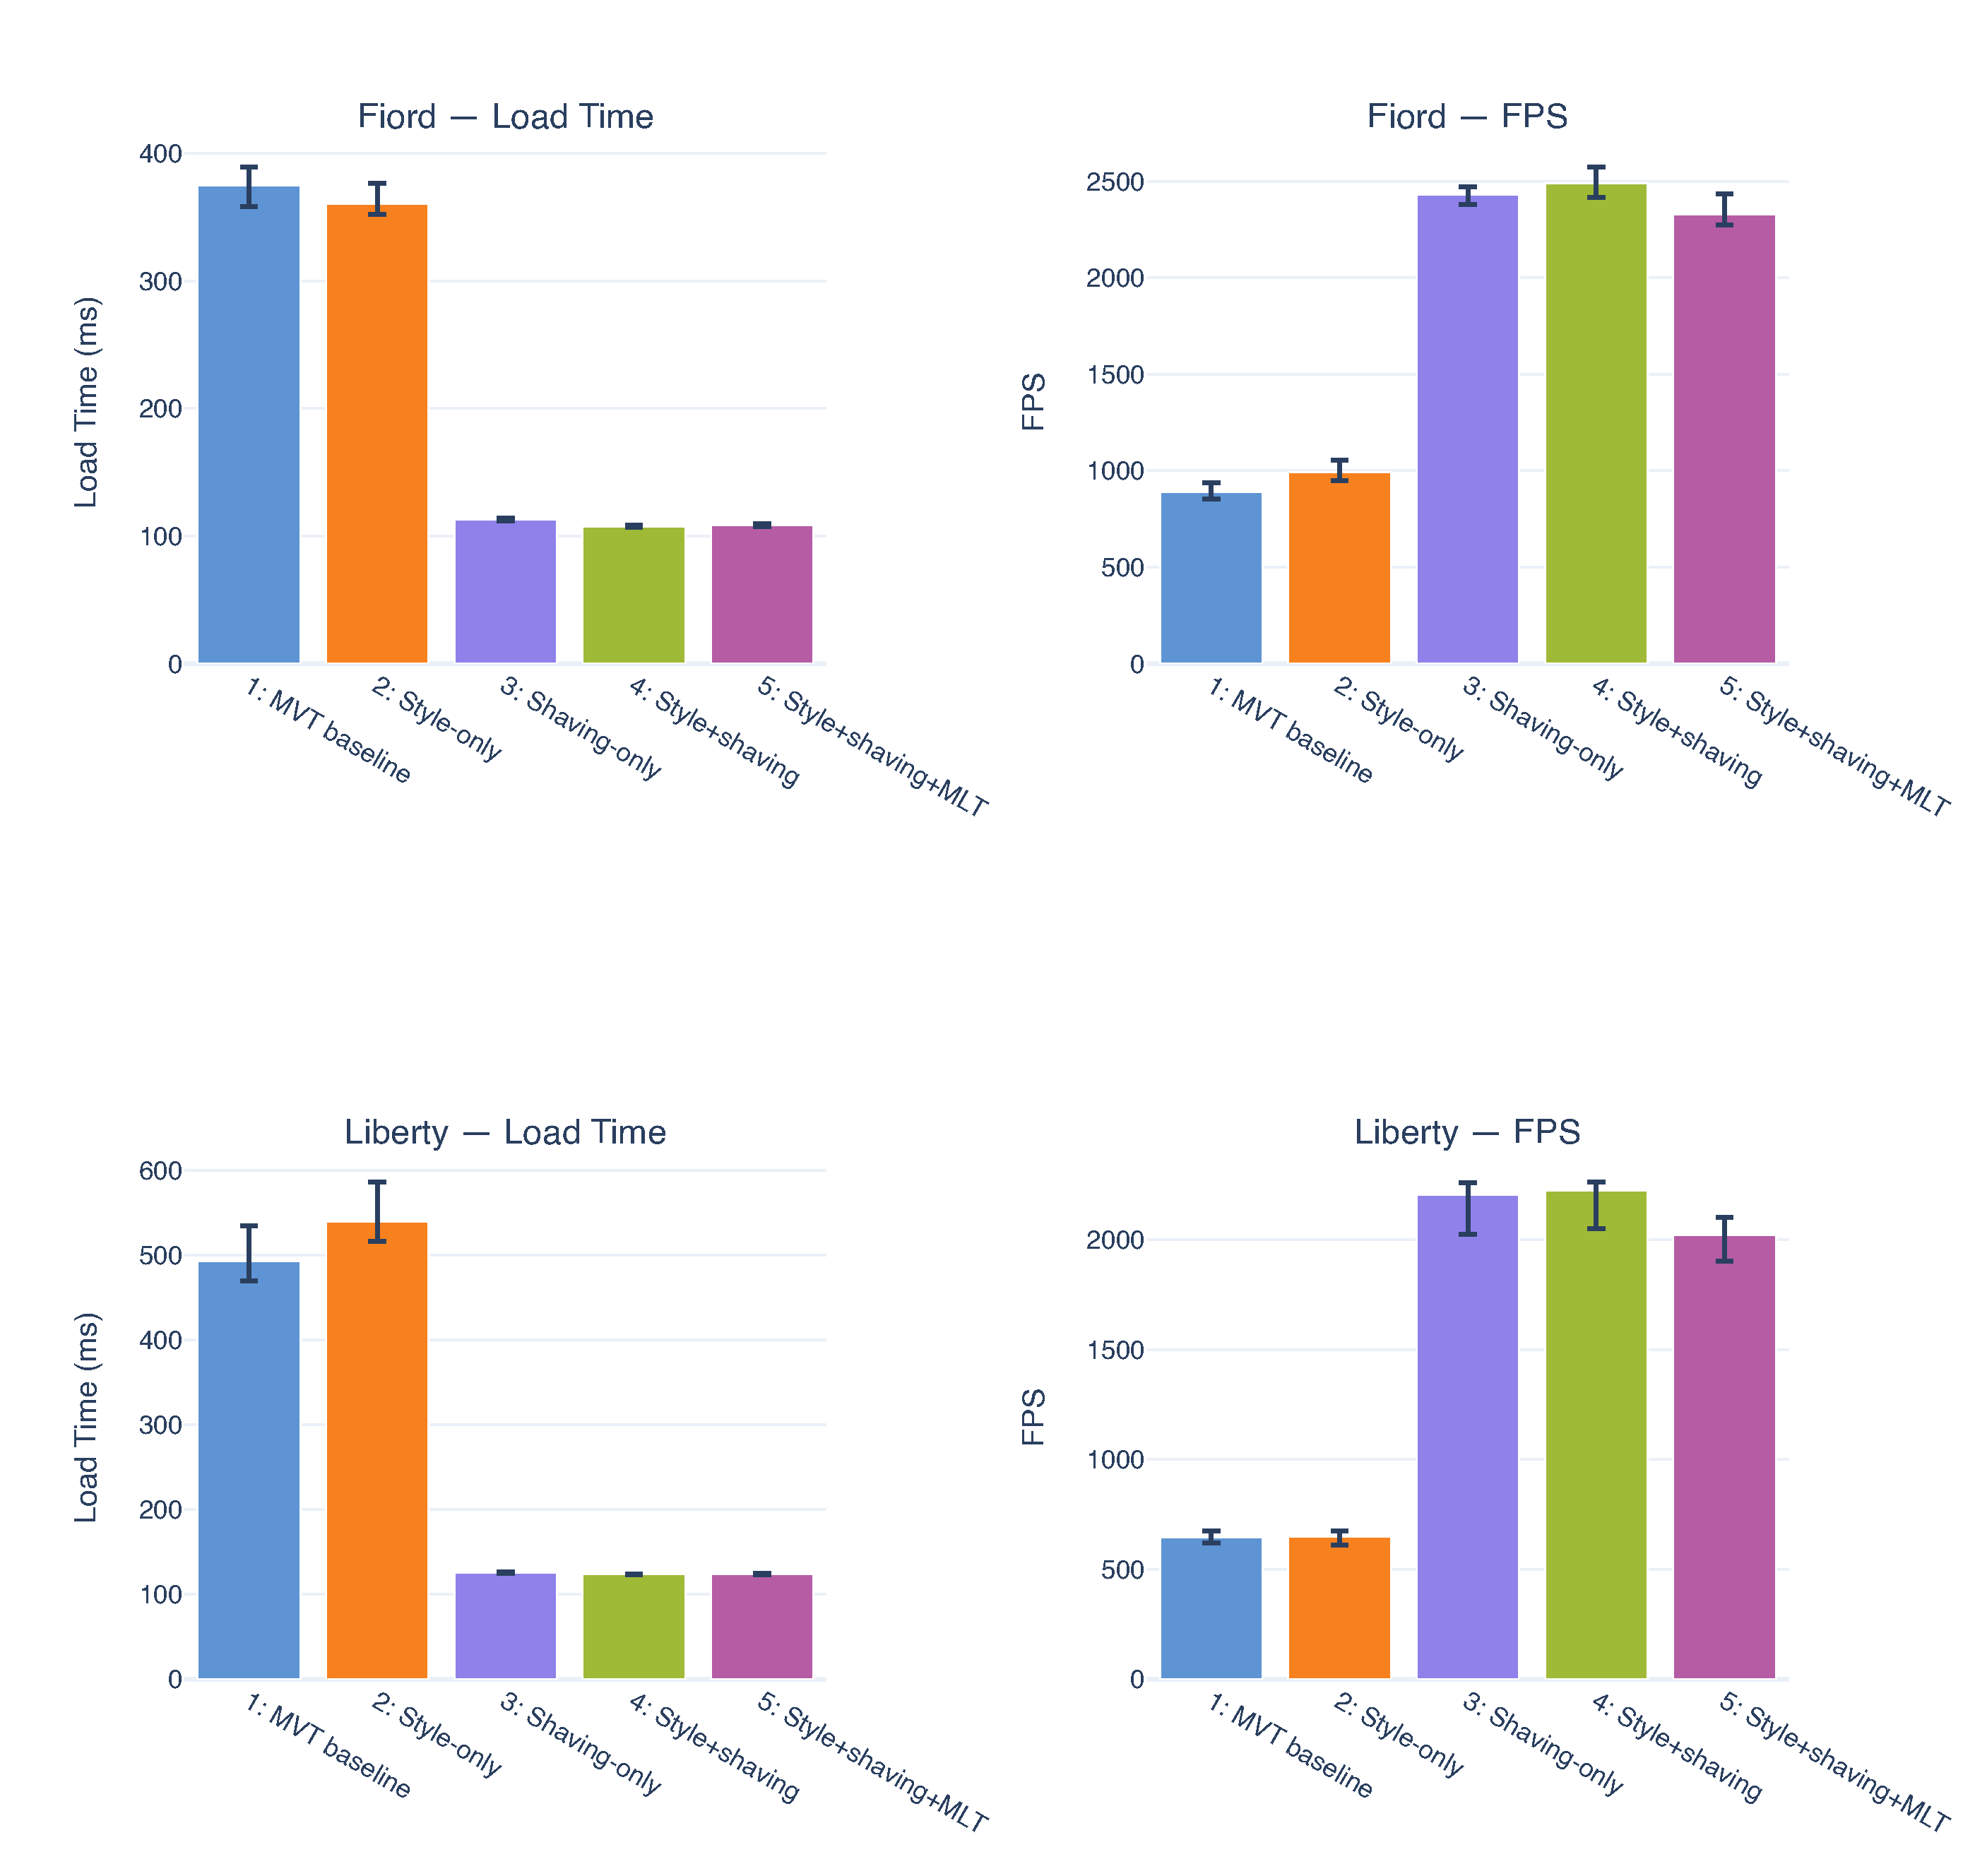
\includegraphics[width=0.9\linewidth]{figures/rendering_metrics_mlt.pdf}
    \caption{Rendering metrics (load time, \ac{FPS}) across configurations~1-5, enabling direct comparison with Experiments~1-2 in the combined analysis. The figure shows the significant drop in both load time and increase in \ac{FPS} for tile shaving, as well as the fact that style-only optimization is ineffective. We also confirm the \ac{MLT} implementation to sligtly decrease performance because the current implementation still internally converts to \ac{MVT}}
    \label{fig:rendering_metrics_mlt}
\end{figure}


\subsection{Results: Encoding the Shaved Data}\label{sub:mlt_encoding_results}

Once shaving has fixed what data survives, the encoding stage determines whether those savings reach the wire.
\cref{fig:shaving_effectiveness_per_zoom} plots total tile size per zoom level for both \ac{MVT} and \ac{MLT}-Rust, with and without shaving via the Liberty advisory.
The gap between each format and its shaved counterpart quantifies the data removed by the pruning advisory; the gap between \ac{MVT}-shaved and \ac{MLT}-Rust-shaved quantifies the additional contribution of columnar encoding on the already-pruned data.
Both formats benefit from shaving across all compression schemes, confirming that the advisory operates on the data itself rather than relying on format-specific redundancy.
\cref{fig:encoder_comparison} reframes the same evidence as a ratio against the \ac{MVT} baseline, adding the Tremmel \& Zink \ac{MLT}-Java encoder for comparison: the \ac{MLT}-Rust curves remain at roughly $0.6$-$0.8\times$ \ac{MVT} throughout the zoom range, whereas the \ac{MLT}-Java curves drift above $1.0\times$ at several zoom levels under brotli/zstd, underscoring that the gains attributed to the \ac{MLT} format in this thesis come almost entirely from the encoder-side strategy competition and not from the columnar format alone.

\begin{figure}[htbp]
    \centering
    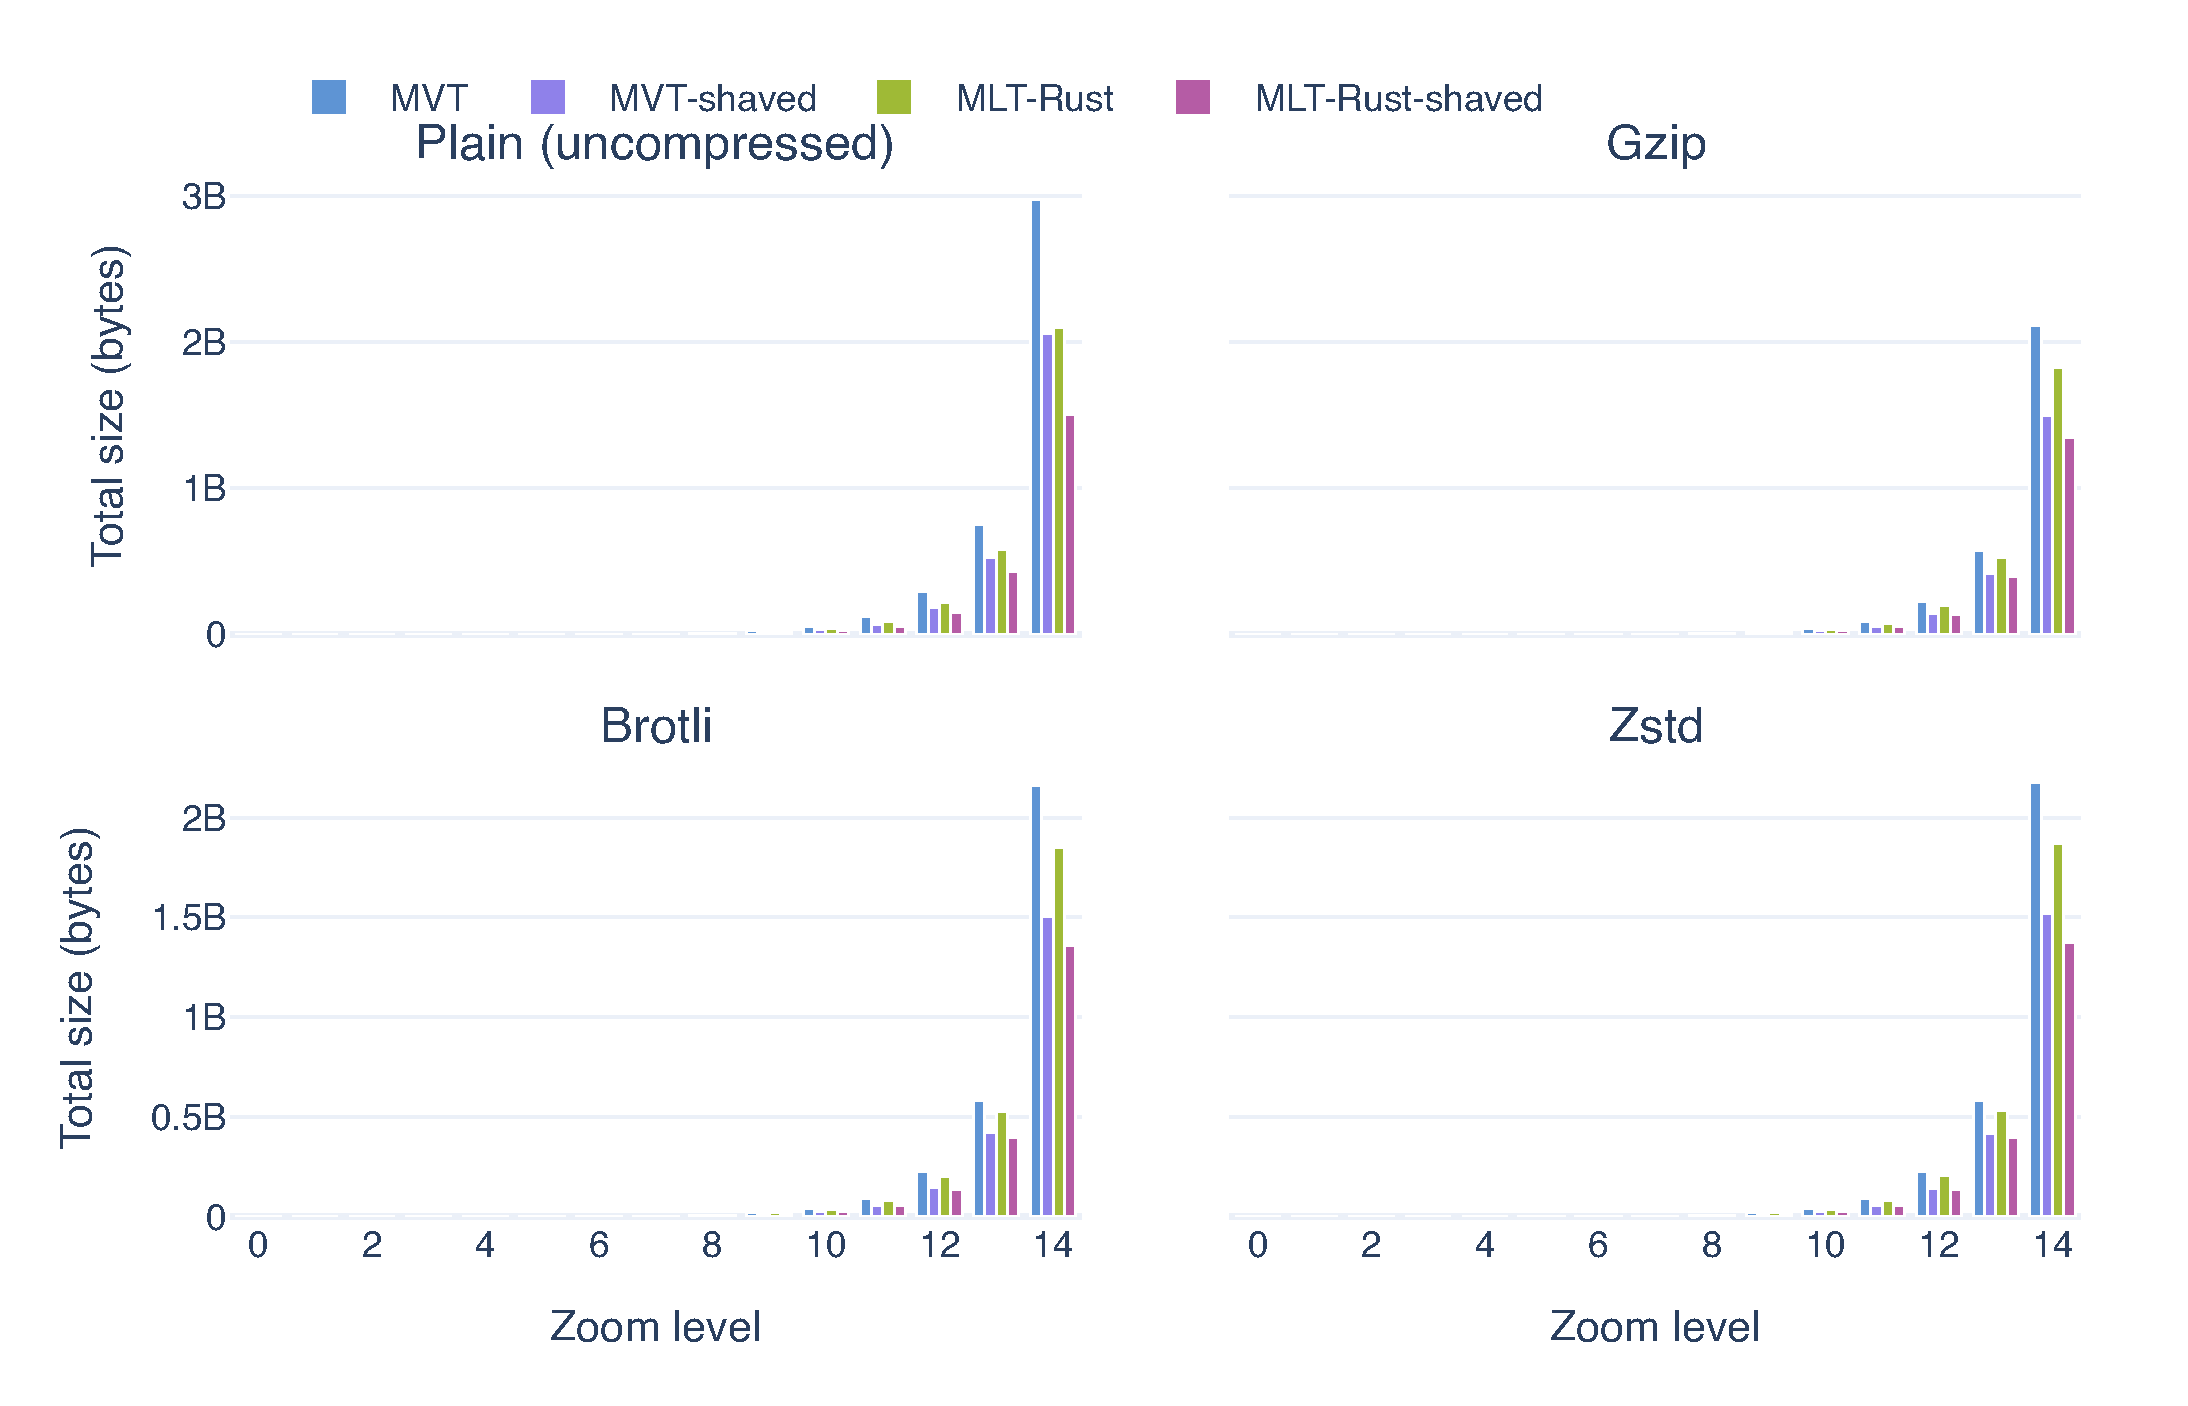
\includegraphics[width=0.9\linewidth]{figures/shaving_effectiveness_per_zoom}
    \caption{Total tile size per zoom level for unshaved and shaved variants of
      both \ac{MVT} and \ac{MLT}-Rust, using the Liberty advisory.  The gap
      between each format and its shaved counterpart quantifies the data removed
      by the pruning advisory; the gap between \ac{MVT}-shaved and
      \ac{MLT}-Rust-shaved quantifies the additional contribution of columnar
      encoding}
    \label{fig:shaving_effectiveness_per_zoom}
\end{figure}

\paragraph{Isolating the contribution of the Rust encoder's strategy selection}
To separate the contribution of the multi-strategy competition (this work) from that of the \ac{MLT} format as proposed by Tremmel and Zink~\cite{tremmelMapLibreTileNext2025b}, we report in \cref{fig:encoder_comparison} both a per-zoom breakdown and the total encoded size of the Germany OpenMapTiles tileset (zoom~0-14, \num{256588} tiles) under three encoders - \ac{MVT} (the row-oriented protobuf baseline), \ac{MLT}-Java (the reference columnar encoder from Tremmel and Zink, used as the \ac{MLT} baseline), and \ac{MLT}-Rust (this thesis' encoder with sort-strategy competition, per-stream profiling, and shared-dictionary clustering) - and across four wire compressions (none, gzip-9, Brotli-11, zstd-22).

\begin{figure}[htbp]
\centering
    \begin{subfigure}[t]{0.95\linewidth}
        \centering
        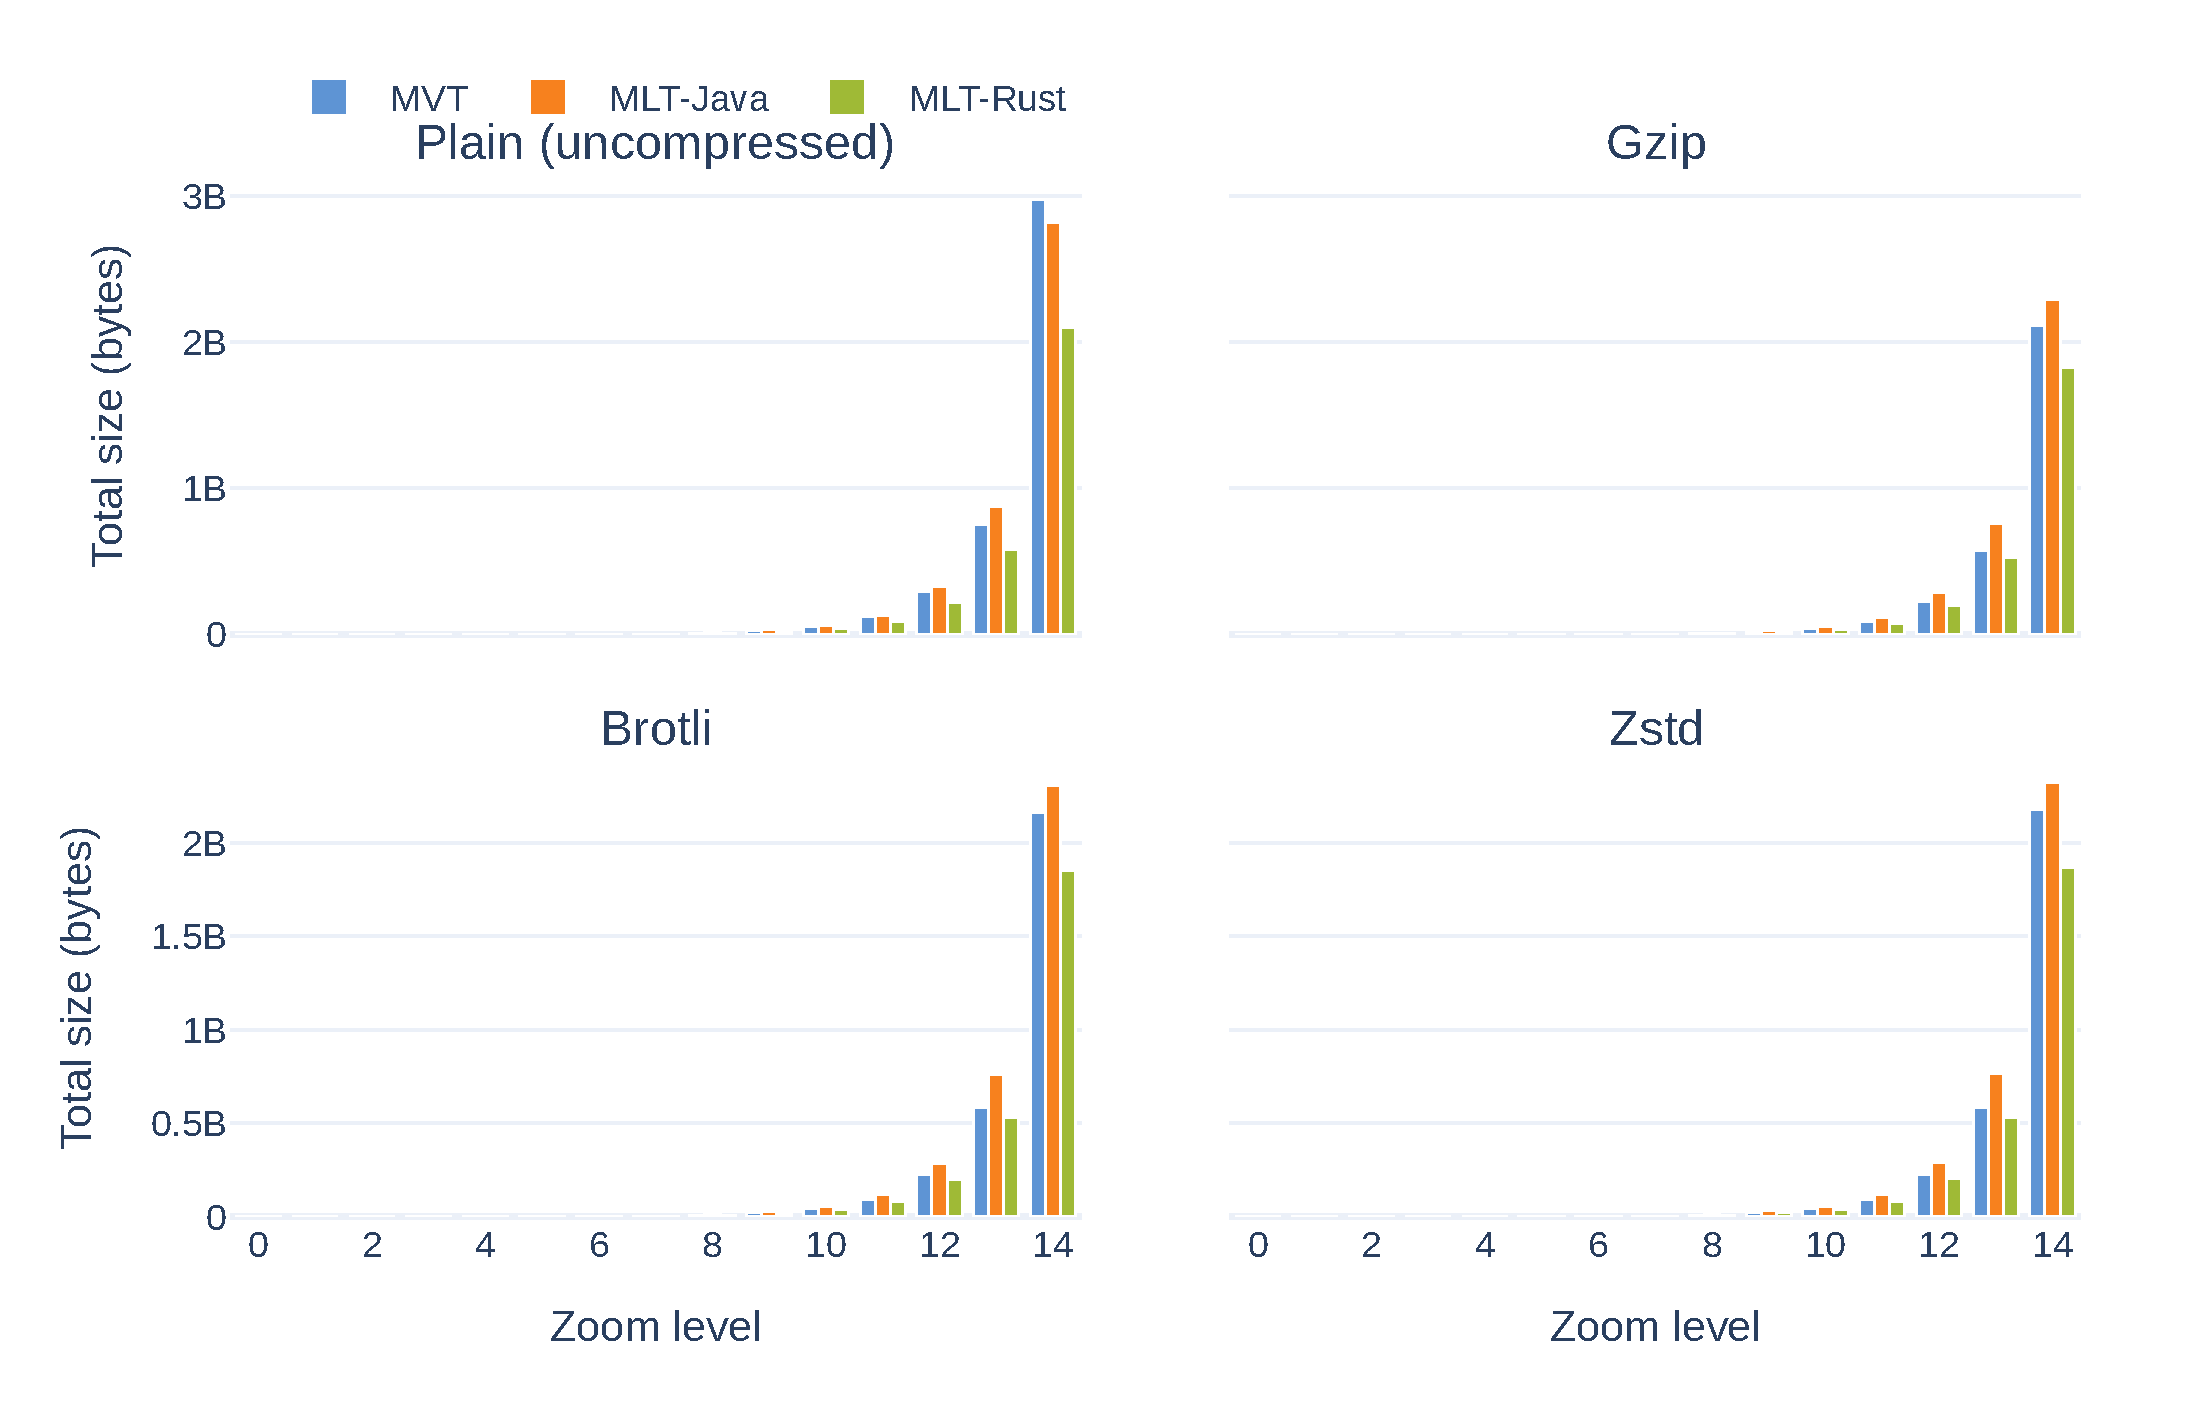
\includegraphics[width=\linewidth]{figures/encoder_comparison_per_zoom}
        \caption{Per-zoom total tile size for the three encoders under four wire compressions}
        \label{fig:encoder_comparison_per_zoom}
    \end{subfigure}

    \vspace{1em}

    \begin{subfigure}[t]{\linewidth}
        \centering
        \begin{tblr}{colspec={l r r r r}, rows={font=\small}, row{1}={font=\small\bfseries}}
        \toprule
        Encoder & Plain (GB) & gzip (GB) & Brotli (GB) & zstd (GB) \\
        \midrule
        \ac{MVT}              & 4.24 & 3.08 & 3.13 & 3.16 \\
        \ac{MLT}-Java baseline & 4.26 & 3.54 & 3.57 & 3.60 \\
        \ac{MLT}-Rust (our work) & \textbf{3.06} &  \textbf{2.70} &  \textbf{2.72} &  \textbf{2.75} \\
        \midrule
        $\Delta$ Rust vs.\ Java & $-28.3\%$ & $-23.8\%$ & $-23.7\%$ & $-23.6\%$ \\
        $\Delta$ Rust vs.\ \ac{MVT} & $-27.9\%$ & $-12.3\%$ & $-13.1\%$ & $-12.9\%$ \\
        \bottomrule
        \end{tblr}
        \caption{Total tileset size for the three encoders under four wire compressions.
          The \ac{MLT}-Java column reports the baseline from~\cite{tremmelMapLibreTileNext2025b}, updated with encoding improvements backported from the Rust encoder development (correct delta-zigzag sequencing, \ac{RLE} viability checks, \ac{FSST} thresholds);
          the \ac{MLT}-Rust column reports the Rust encoder developed in this thesis}
        \label{tab:mvt_mlt_comparison}
    \end{subfigure}
\caption[Encoder comparison: per-zoom breakdown and total tileset size]{Encoder comparison for the Germany OpenMapTiles tileset (zoom~0-14, \num{256588} tiles). \ac{MLT}-Rust (this work) achieves \qty{28.3}{\percent} smaller total size than the \ac{MLT}-Java baseline under no wire compression; the Java encoder drifts above \ac{MVT} size at several zoom levels under Brotli/zstd, whereas the Rust encoder remains below \ac{MVT} throughout.}
\label{fig:encoder_comparison}
\end{figure}

The headline number is the \qty{28.3}{\percent} reduction the Rust encoder achieves over the \ac{MLT}-Java baseline under no wire compression, confirming that the sort-strategy competition, per-stream profiler, and shared-dictionary clustering add substantial savings over a columnar encoder that simply picks a fixed encoding plan.
The Java baseline we use here already incorporates encoding improvements backported from the Rust encoder's development (correct delta-zigzag sequencing, \ac{RLE} viability checks, \ac{FSST} thresholds), so the \qty{28}{\percent} isolates the contribution of the automatic strategy selection - sort competition, per-stream profiling, and MinHash-based shared-dictionary clustering - over a correctly-implemented fixed-plan encoder, rather than conflating bug fixes with the innovation we want to attribute to.

The finding in the table that is easiest to overlook, and the one we found most uncomfortable when we first plotted it, is that the \ac{MLT}-Java baseline is \emph{worse} than gzip-compressed \ac{MVT} (\qty{3.54}{\giga\byte} vs.\ \qty{3.08}{\giga\byte}).
General-purpose LZ77-family compressors already exploit most of the row-level redundancy in the protobuf wire format, and a columnar encoder that uses fixed per-column schemes cannot keep up.
The data-driven strategy selection in the Rust encoder reclaims this gap and goes past it: \ac{MLT}-Rust under gzip is \qty{12.3}{\percent} smaller than \ac{MVT} under gzip, and the advantage holds (\qty{12.9}{\percent}) even against zstd-22, the strongest general-purpose compressor in the comparison.

The relative gap between Rust and Java is roughly constant across all four compressors (\qty{-23}{\percent} to \qty{-28}{\percent}).
This stability is consistent with the profiler capturing genuine redundancy that general-purpose compressors miss, but it could equally reflect that the profiler removes the same redundancy the compressors would have.
The cleaner evidence for the profiler's value is the absolute comparison: \ac{MLT}-Rust uncompressed (\qty{3.06}{\giga\byte}) is already smaller than \ac{MVT}+gzip (\qty{3.08}{\giga\byte}), confirming that per-stream encoding captures type-specific redundancy that LZ77-family compressors miss on the interleaved protobuf byte stream.
This directly answers the question we posed at the start of \cref{sec:exp_mlt}: the \ac{MLT}-Rust contribution lives in the joint strategy-selection layer that sits on top of the columnar format, not in the format alone.

\paragraph{Scope of the encoder contribution}
We measured the \qty{28}{\percent} reduction reported in \cref{tab:mvt_mlt_comparison} on the \emph{unshaved} Germany tileset, so it is an encoder-only improvement, independent of the style-driven optimizations.
It reflects the combined effect of sort-strategy competition, per-stream profiling, and shared-dictionary clustering; these three mechanisms are tightly coupled (sort order affects column distributions, which affect profiling decisions), so a per-mechanism decomposition is not feasible without re-engineering the encoder.
This result is complementary to, but separate from, the style-data bridge: style-driven tile shaving reduces tile content before encoding, while the encoder improvements reduce the encoded size of whatever content remains.
The two contributions stack (shaved tiles encoded with the Rust encoder are smaller than shaved tiles encoded with the Java baseline), but they address orthogonal sources of redundancy.

\paragraph{Why not just apply zstd to \acs{MVT}?}
A natural objection is that general-purpose compressors such as zstd-22 or Brotli-11 should be sufficient: if compression is the goal, simply applying the strongest available compressor to the existing \ac{MVT} wire format would avoid the complexity of a columnar encoder entirely.
\Cref{tab:mvt_mlt_comparison} answers this directly.
\ac{MVT} under zstd-22 yields \qty{3.16}{\giga\byte} for the Germany tileset, whereas \ac{MLT}-Rust under the same compressor yields \qty{2.75}{\giga\byte} - a \qty{12.9}{\percent} reduction.
We attribute this to a structural difference: a general-purpose compressor sees the interleaved, heterogeneous protobuf byte stream and must discover redundancy across mixed data types.
A columnar encoder, by contrast, groups homogeneous values - all road classes in one stream, all vertex deltas in another - and each stream compresses more effectively under lightweight per-type codecs (delta-\acs{RLE} for monotonic integers, dictionary encoding for low-cardinality strings, \ac{FSST} for high-cardinality strings) than a monolithic LZ77-family compressor can achieve on the interleaved byte stream.
The columnar advantage is preserved \emph{after} applying the same general-purpose compressor on top: the per-column codecs have already removed most of the type-specific redundancy, so the post-hoc compressor has less work to do but starts from a lower baseline.
This finding is consistent with the columnar-database literature, where per-column lightweight encoding consistently outperforms row-level block compression even when the block compressor is state-of-the-art~\cite{kuschewskiBtrBlocksEfficientColumnar2023}.

\paragraph{Decoder cost}
A legitimate concern for any multi-encoding scheme is that the client must pay the decoder cost, which can erode the transfer savings on mobile or battery-constrained targets.
We engineered the decoder to amortise its per-column dispatch over per-feature work (\cref{sub:encoding_strategies}); empirically, our benchmarks on the full Germany tileset show end-to-end rendering metrics comparable to or better than \ac{MVT} at matched workloads, and we see no negative effect in the sustained frame-time metrics of \cref{sub:combined_marginal}.


\paragraph{Decoding throughput}
To isolate decoding latency from the browser-based rendering benchmark (where it is embedded in \texttt{loadMs}), we use Criterion micro-benchmarks to measure full-decode throughput for \ac{MLT}-Rust vs.\ \ac{MVT} with and without transport compression.
Each benchmark parses the tile header and materialises all features and properties; \ac{MVT} variants include gzip decompression in the measured path.
\Cref{tab:decode_throughput} reports the results on a representative subset of the OpenMapTiles fixture tiles at zoom levels~4, 7, and~13 (100~samples per cell).

\begin{table}[htbp]
\centering
\small
\begin{tblr}{colspec={l r r r}, rows={font=\small}, row{1}={font=\small\bfseries}}
\toprule
Format & Zoom~4 & Zoom~7 & Zoom~13 \\
\midrule
\ac{MLT}-Rust & \qty{5.73}{\milli\second} & \qty{19.4}{\milli\second} & \qty{4.09}{\milli\second} \\
\ac{MVT}+gzip & \qty{47.6}{\milli\second} & \qty{103}{\milli\second} & \qty{18.7}{\milli\second} \\
\ac{MVT} (uncompressed) & \qty{44.2}{\milli\second} & \qty{90.6}{\milli\second} & \qty{16.5}{\milli\second} \\
\midrule
Speedup (vs.\ gzip) & $8.3\times$ & $5.3\times$ & $4.6\times$ \\
\bottomrule
\end{tblr}
\caption{Full-decode latency for \ac{MLT}-Rust vs.\ \ac{MVT} on OpenMapTiles fixture tiles, measured by Criterion micro-benchmarks (100~samples per cell).
\ac{MLT}-Rust achieves \numrange{96}{134}\,MiB/s decode throughput vs.\ \numrange{15}{23}\,MiB/s for \ac{MVT}+gzip (measured over wire-format input size)}
\label{tab:decode_throughput}
\end{table}

The \ac{MLT} decoder's columnar layout enables selective column access and avoids the per-feature tag-parsing overhead of protobuf, which accounts for the speedup even before transport decompression is considered: \ac{MLT}-Rust is $4.0$-$7.7\times$ faster than uncompressed \ac{MVT}.
These micro-benchmark results complement the browser-based \texttt{loadMs} metric by providing an isolated measurement of the decoding-latency axis of Research Goal~R3, even though they are not 1:1 applicable because we do not use the Rust decoder in \texttt{maplibre-gl-js}.

\subsection{Discussion}\label{sub:mlt_discussion}

Tile shaving alone cuts pooled median load time by \qty{71.5}{\percent} and lifts \ac{FPS} by \qty{184}{\percent}, while style-only passes contribute \qty{-4.1}{\percent} on load; the two channels compose additively, not synergistically.
We discuss why the channels stay additive, the cache-fragmentation trade-off that style-dependent tiles create on shared \acsp{CDN}, and the geometry-simplification axis we leave out of scope.

\paragraph{Tile shaving dominates; style passes assist additively}
The headline finding of this experiment is that tile shaving is the dominant contributor to load-time and transfer-size improvements, while style-level passes provide a modest, additive assist.
Dead layer elimination (Experiment~2) removes style layers whose filters are unsatisfiable.
Each removed layer reduces the set of referenced properties in the pruning advisory, which in turn can eliminate columns from the encoded tile.
Metadata refinement tightens zoom bounds, which causes the advisory to mark additional zoom levels as unused, potentially eliminating tiles entirely.
However, the aggregate data shows no super-additive interaction at the median level (\cref{sub:mlt_results}): the combined style+shaving reduction is approximately the sum of the individual reductions, not greater.
We therefore best understand the style-level passes as useful enablers - simplifying the advisory and improving code quality - rather than as co-equal partners in a synergistic cascade.
The encoding stage that follows benefits from this enabling effect: shaved data presents longer runs and smaller dictionaries to the per-stream profiler, which is why we place the multi-strategy competition in the same pipeline rather than as a standalone encoder paper.

\paragraph{Style-dependent tile sizes}
A consequence of style-driven shaving is that different styles produce different tile sizes from the same source data.
To quantify this variation, we ran the full shaving pipeline (optimize with all passes, generate pruning advisory, apply advisory as \ac{MVT}) on the same Germany tileset (\qty{3.07}{\giga\byte}, OpenMapTiles schema, zoom levels 0-14) for each of the 11 \ac{OMT}-compatible styles in the benchmark corpus.
\cref{fig:tile_shave_per_style} shows the results: tile-data reductions range from \qty{19.8}{\percent} (Bright) to \qty{46.3}{\percent} (Toner), with a median of \qty{29.0}{\percent}.
Styles that reference fewer source-layers and property columns - such as Toner (monochrome, road/water/boundary only) and Americana (focused on shield and label rendering) - leave more tile data unused, enabling the advisory to strip more columns and features.
Conversely, broad-coverage styles like Bright and OSM~Bright reference most of the tileset's property columns, limiting the shaving headroom.
We see this observation as highlighting a fundamental trade-off: there is no single optimal tile - the optimal encoding depends on the rendering style, which is a design choice.

\begin{figure}[htbp]
    \centering
    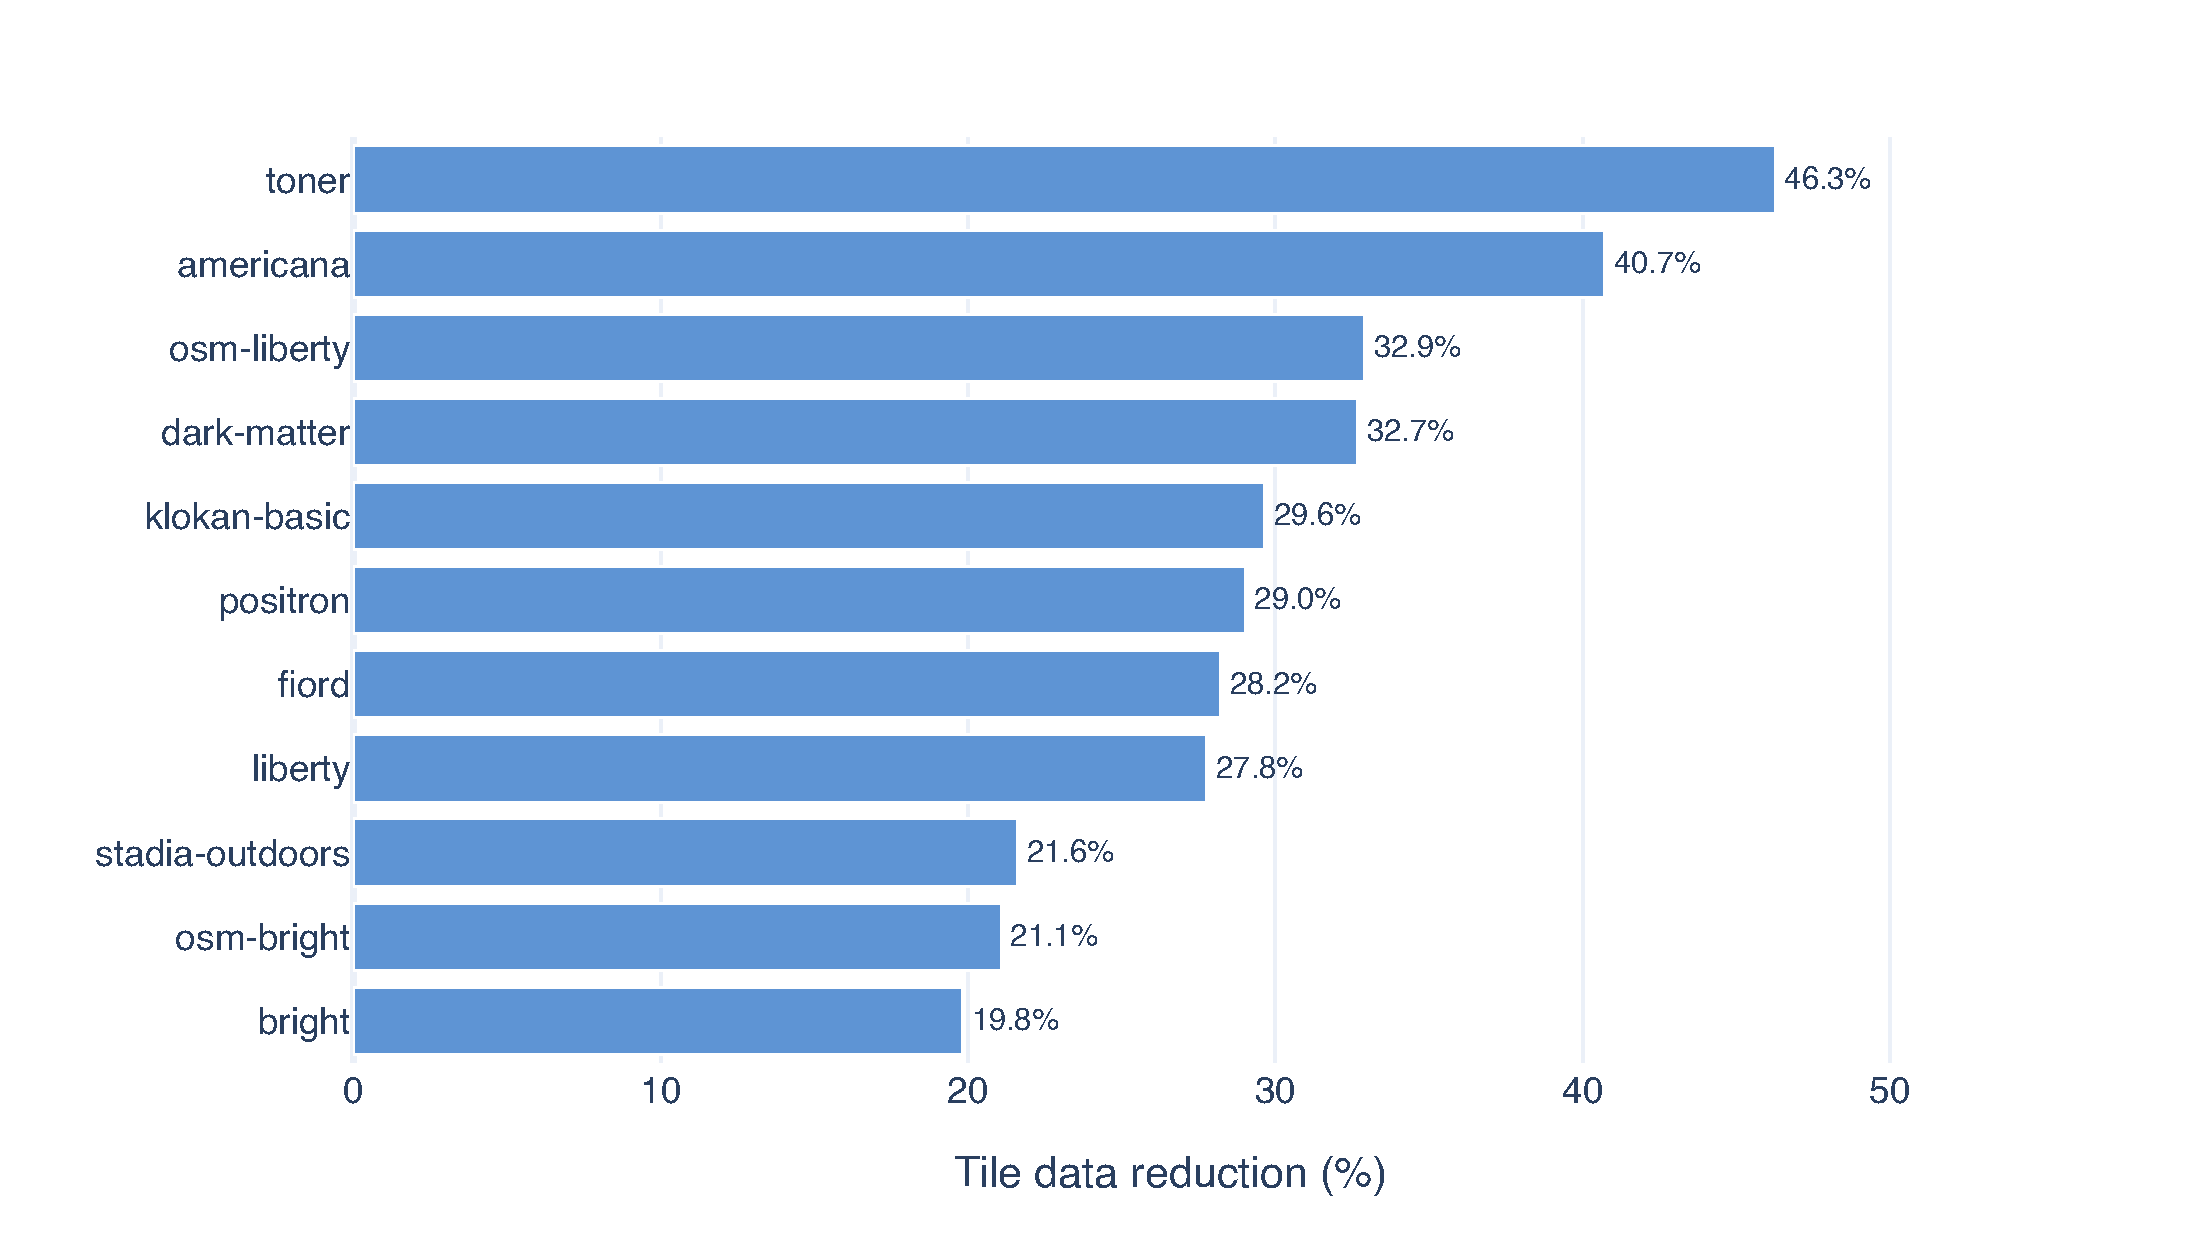
\includegraphics[width=0.8\linewidth]{figures/tile_shave_per_style}
    \caption{On-Wire data reduction from style-driven \ac{MVT} shaving across 11 \ac{OMT}-compatible styles, applied to the same \qty{3.07}{\giga\byte} Germany tileset.  Styles that reference fewer source-layers and properties achieve larger reductions}
    \label{fig:tile_shave_per_style}
\end{figure}

\paragraph{Cache fragmentation trade-off}
A direct operational consequence of style-dependent tiles is that shared \ac{CDN} caching is partially defeated: two styles that served identical tiles under \ac{MVT} now fetch distinct shaved variants, and a \ac{CDN} must either key its cache on (tile, style) pairs or accept that a hit on one style is a miss on another.
The break-even point depends on the ratio of per-style rendering cost savings to the amplified origin fetch rate.
For deployments where a single style dominates traffic, style-driven shaving is strictly beneficial; for multi-tenant tile servers hosting dozens of styles, operators should apply shaving per style and cache the resulting tile variants independently (the approach of Mapbox's closed-source \enquote{style-optimized vector tiles} service~\cite{StyleoptimizedVectorTiles}).
A hybrid strategy - serving raw \ac{MVT} for uncommon styles and shaved \ac{MLT} for a small set of \enquote{canonical} styles - captures most of the per-tile savings while bounding cache-key explosion.

We frame the decision with a per-style break-even model.
Because \ac{MVT} and \ac{MLT} cannot coexist within a single style's vector-tile source, every style is either served as shaved \ac{MLT} (with its own \emph{(tile, style)} cache-key namespace) or as raw \ac{MVT} (sharing cache slots with all other \ac{MVT}-served styles).
The choice is usually binary per style (given most styles only have one vector tile source), and the operational question is which styles belong in which group.

Let $r$ denote the per-tile rendering-time saving from shaving (load-time reduction divided by the number of fetched tiles), $C_f$ the origin fetch cost per cache miss, $\lambda_i$ the aggregate request rate to style $i$, $N$ the number of distinct tiles, and $\mathcal{M}$ the subset of styles served as \ac{MVT} with pooled rate $\Lambda_\mathcal{M} = \sum_{i \in \mathcal{M}} \lambda_i$.
Let $h(\mu)$ denote the steady-state hit rate of a cache slot accessed at rate $\mu$ on the shared edge cache; under \ac{LRU}, $h$ is monotonically increasing in $\mu$ and saturates near $1$ for popular content.
A style-$j \in \mathcal{M}$ request hits the per-tile pooled slot at rate $\Lambda_\mathcal{M}/N$, while a style served as shaved \ac{MLT} hits its own \emph{(tile, style)} slot at rate only $\lambda_i/N$.
Moving style $i$ from $\mathcal{M}$ to the \ac{MLT}-served set is net-beneficial when
\[
    r \;>\; \big[\, h(\Lambda_\mathcal{M}/N) - h(\lambda_i/N) \,\big] \cdot C_f
\]
where the bracketed \emph{hit-rate gap} measures the cache warmth that style $i$ surrenders by leaving the pool.
The decision depends on style $i$'s share of pool traffic, not on the total number of styles served.

We identify two practically meaningful regimes.
A \emph{dominant style} ($\lambda_i$ comparable to $\Lambda_\mathcal{M}$) sees a near-zero gap, since the pool was already warmed almost entirely by its own traffic, and any positive $r$ justifies shaving.
A \emph{long-tail style} ($\lambda_i \ll \Lambda_\mathcal{M}$) sees a gap that approaches the full pooled hit rate $h(\Lambda_\mathcal{M}/N)$, because its private cache cannot self-warm on its own thin traffic and reverts to near-cold-start behavior.
With our benchmark values ($r \approx \qty{3}{\milli\second}$ per tile, $C_f \approx \qty{25.8}{\milli\second}$ under the Rusan et al.~\cite{rusanAssessmentPacketLatency2015} $\frac{\text{tile size}}{\qty{30}{\mega\bit\per\second}} + \frac{\qty{25}{\milli\second}}{2}$ server-side-throttle for a \qty{50}{\kilo\byte} average tile) and a representative pooled hit rate $h(\Lambda_\mathcal{M}/N) \approx 0.9$ for popular tile content, the maximum tolerable hit-rate gap is $r/C_f \approx 11.6\%$.

Under typical \ac{LRU} dynamics this in turn requires the style to hold a majority share of pool traffic before it can be shaved profitably.
We draw the corollary of the hybrid pattern from this:
shave the one or two canonical styles that dominate the pool, and leave the long tail on raw \ac{MVT}.
Traffic concentration drives this recommendation, not style count - a server hosting fifty styles with one \qty{70}{\percent}-share dominant style behaves the same as one hosting five with the same concentration.
Our model omits spatial locality and the second-order effect that peeling the dominant style off the pool cools the cache further for the remaining \ac{MVT}-served styles, both of which would only sharpen the recommendation.

\paragraph{Geometry simplification is out of scope}
A complementary direction we do not explore in this thesis is geometry-level pruning - coordinate precision reduction, Visvalingam~\cite{visvalingamLineGeneralisationRepeated1993} or Douglas-Peucker~\cite{douglasALGORITHMSREDUCTIONNUMBER1973} simplification, and polygon topology coalescing - which is the principal lever used by upstream generators such as Tippecanoe\footnote{\url{https://github.com/felt/tippecanoe}, last accessed 2026-04-21} and Planetiler\footnote{\url{https://github.com/onthegomap/planetiler}, last accessed 2026-04-21}.
These techniques typically deliver larger absolute savings than attribute-column pruning, but they interact non-trivially with style-defined visual thresholds (line width, dash pattern length, label anchor placement) and would violate the pixel-identity soundness criterion established in \cref{sec:problem_statement}.
Style-driven geometry simplification - choosing a simplification tolerance that is demonstrably below the smallest visible feature at each zoom level - is an interesting direction for future work but we do not pursue it here.
We therefore quantify the size reductions achievable \emph{without} touching geometry at all, which understates the total optimizations headroom a production pipeline could reach by composing this work with an upstream simplifier.

\section{Cross-Style Generalisation}\label{sec:exp_cross_style}
\begin{keytakeaways}
\item Static-only passes generalize: median \qty{31.4}{\percent} raw reduction across 13 unseen styles, none regressed.
\item Initial style size and complexity does not predict reduction ($r = 0.35$, $n = 13$, $p = 0.24$).
\item These numbers are a lower bound - stats-driven and data-level passes were not applied here.
\end{keytakeaways}

\noindent In the preceding experiments we evaluated optimizations effectiveness on the curated benchmarking corpus of 15 styles described in \cref{sub:deep_corpus}.
To assess whether the observed gains generalize, we apply the optimizer to the 13~styles of the Maputnik generalization corpus introduced in \cref{sub:generalization_corpus}.
We use three tiers of breadth because end-to-end rendering benchmarks require tile data and browser automation infrastructure that does not scale to all styles: we benchmark ten deep-corpus styles end-to-end with tile data, eleven \ac{OMT}-compatible styles at the tile-shaving size level, and evaluate thirteen additional styles with static analysis only.

\subsection{Methodology}\label{sub:cross_methodology}

We use static analysis only for the cross-style evaluation: we optimize each style with all passes enabled, and compare the resulting style to the original on size and complexity metrics.
We execute no rendering benchmarks, as the diverse styles reference incompatible tile schemas and tile sources that we cannot uniformly provision.

\subsection{Results}\label{sub:cross_results}

\cref{fig:cross_style_reduction} shows per-style percentage reductions (raw, gzip, Brotli) across the 13 Maputnik styles, sorted by raw reduction; the key question here is whether the distribution clusters tightly around the deep corpus median or fans out with substantial per-style variance.
\cref{fig:cross_style_complexity_scatter} then plots each style's initial complexity against its achievable reduction, testing the hypothesis that verbose institutional styles (the right-hand side of the scatter) have disproportionately more optimizations headroom than already-compact minimal basemaps on the left.

The distribution fans out considerably:
raw reductions range from \qty{3.2}{\percent} (Stadia Outdoors) to \qty{67.7}{\percent} (LocationIQ Streets), with no style regressing.
Under gzip compression the range narrows to \qtyrange{3.9}{22.4}{\percent} (median \qty{11.4}{\percent}), confirming that some of the raw-byte savings overlap with what gzip already captures.
The top reducers - LocationIQ Streets (\qty{67.7}{\percent} raw), Americana (\qty{59.2}{\percent}), and MapTiler Toner (\qty{57.5}{\percent}) - are styles with either verbose filter logic (LocationIQ, Americana) or highly repetitive property structures (Toner).
At the low end, Stadia Outdoors (\qty{3.2}{\percent}) and the two AWS styles (both at \qty{10.6}{\percent}) leave little for the optimizer to remove: the AWS pair shares a codebase of hand-tuned expressions with few redundancies, while Stadia Outdoors is a compact, already-minified basemap.
We observe no statistically significant correlation between initial \ac{AST} node count and reduction ($r = 0.35$, $n = 13$, $p = 0.24$); the sample size is too small for this correlation to be meaningful.  Americana has by far the highest initial complexity (\num{48510} nodes) and is also one of the top three reducers, but it is a single high-leverage point: dropping it flips the sign to $r = -0.54$, underscoring that no stable trend exists at this sample size.

\begin{figure}[htbp]
    \centering
    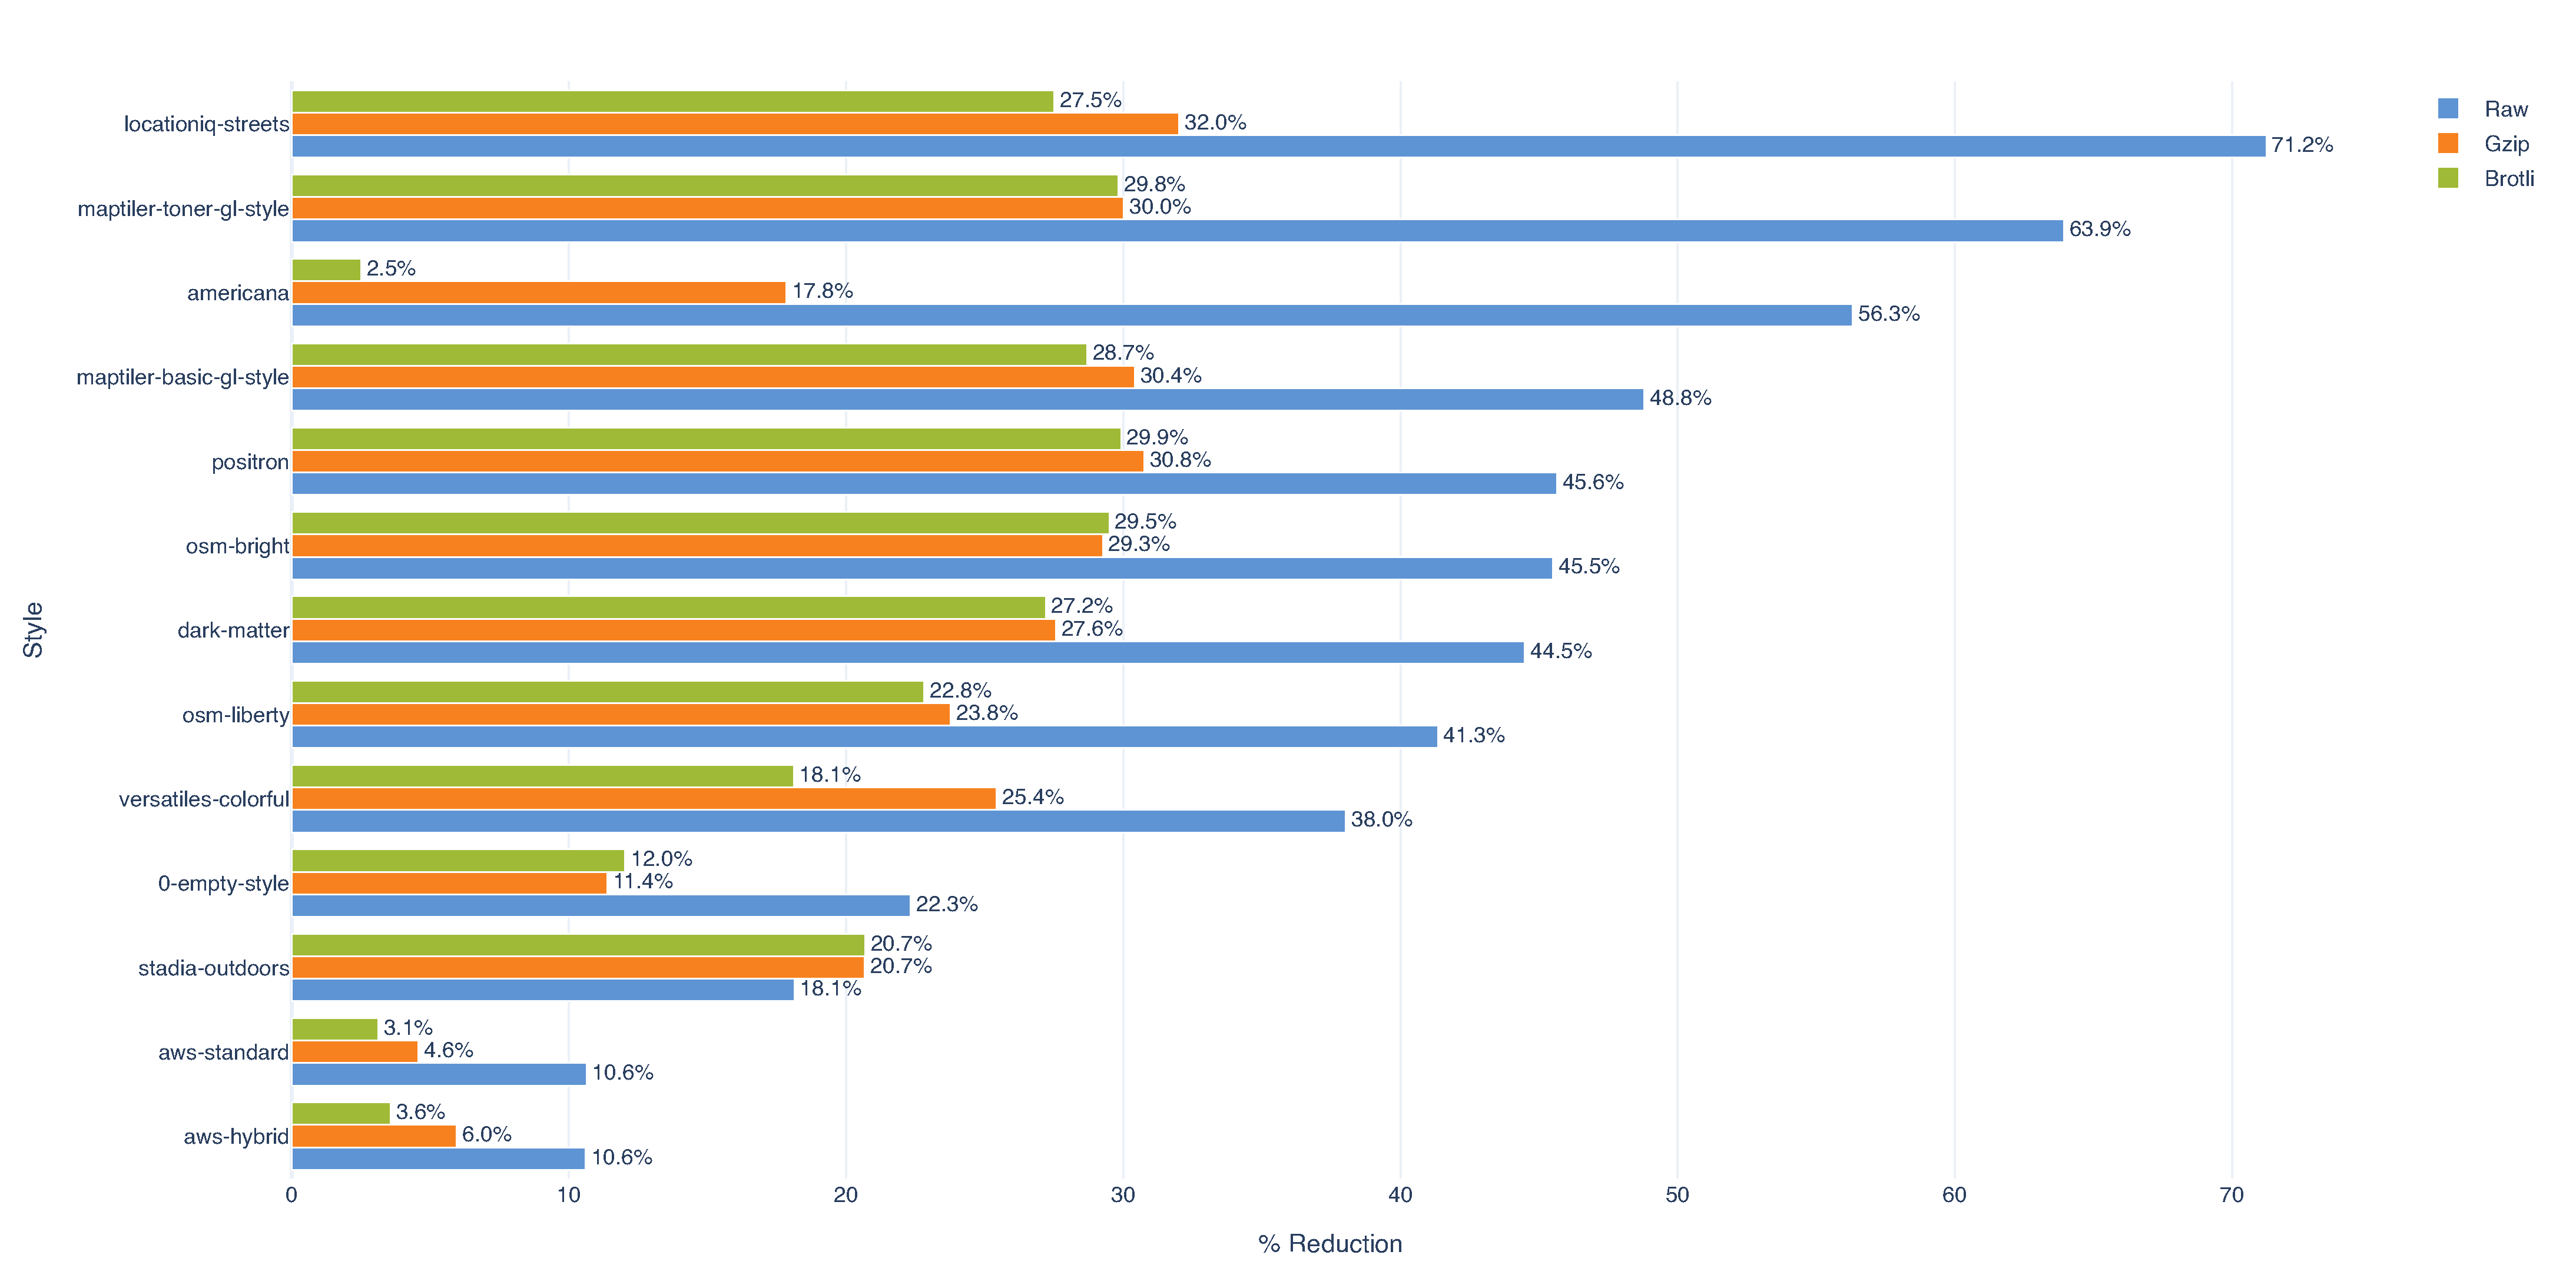
\includegraphics[width=\linewidth]{figures/cross_style_reduction.pdf}
    \caption{Per-style percentage reduction in style size (raw, gzip, Brotli) across the Maputnik generalization corpus; styles are sorted by raw reduction. Raw reductions range from \qty{3.2}{\percent} to \qty{67.7}{\percent}, confirming that automatic optimization yields meaningful gains across styles regardless of origin.}
    \label{fig:cross_style_reduction}
\end{figure}

\begin{figure}[htbp]
    \centering
    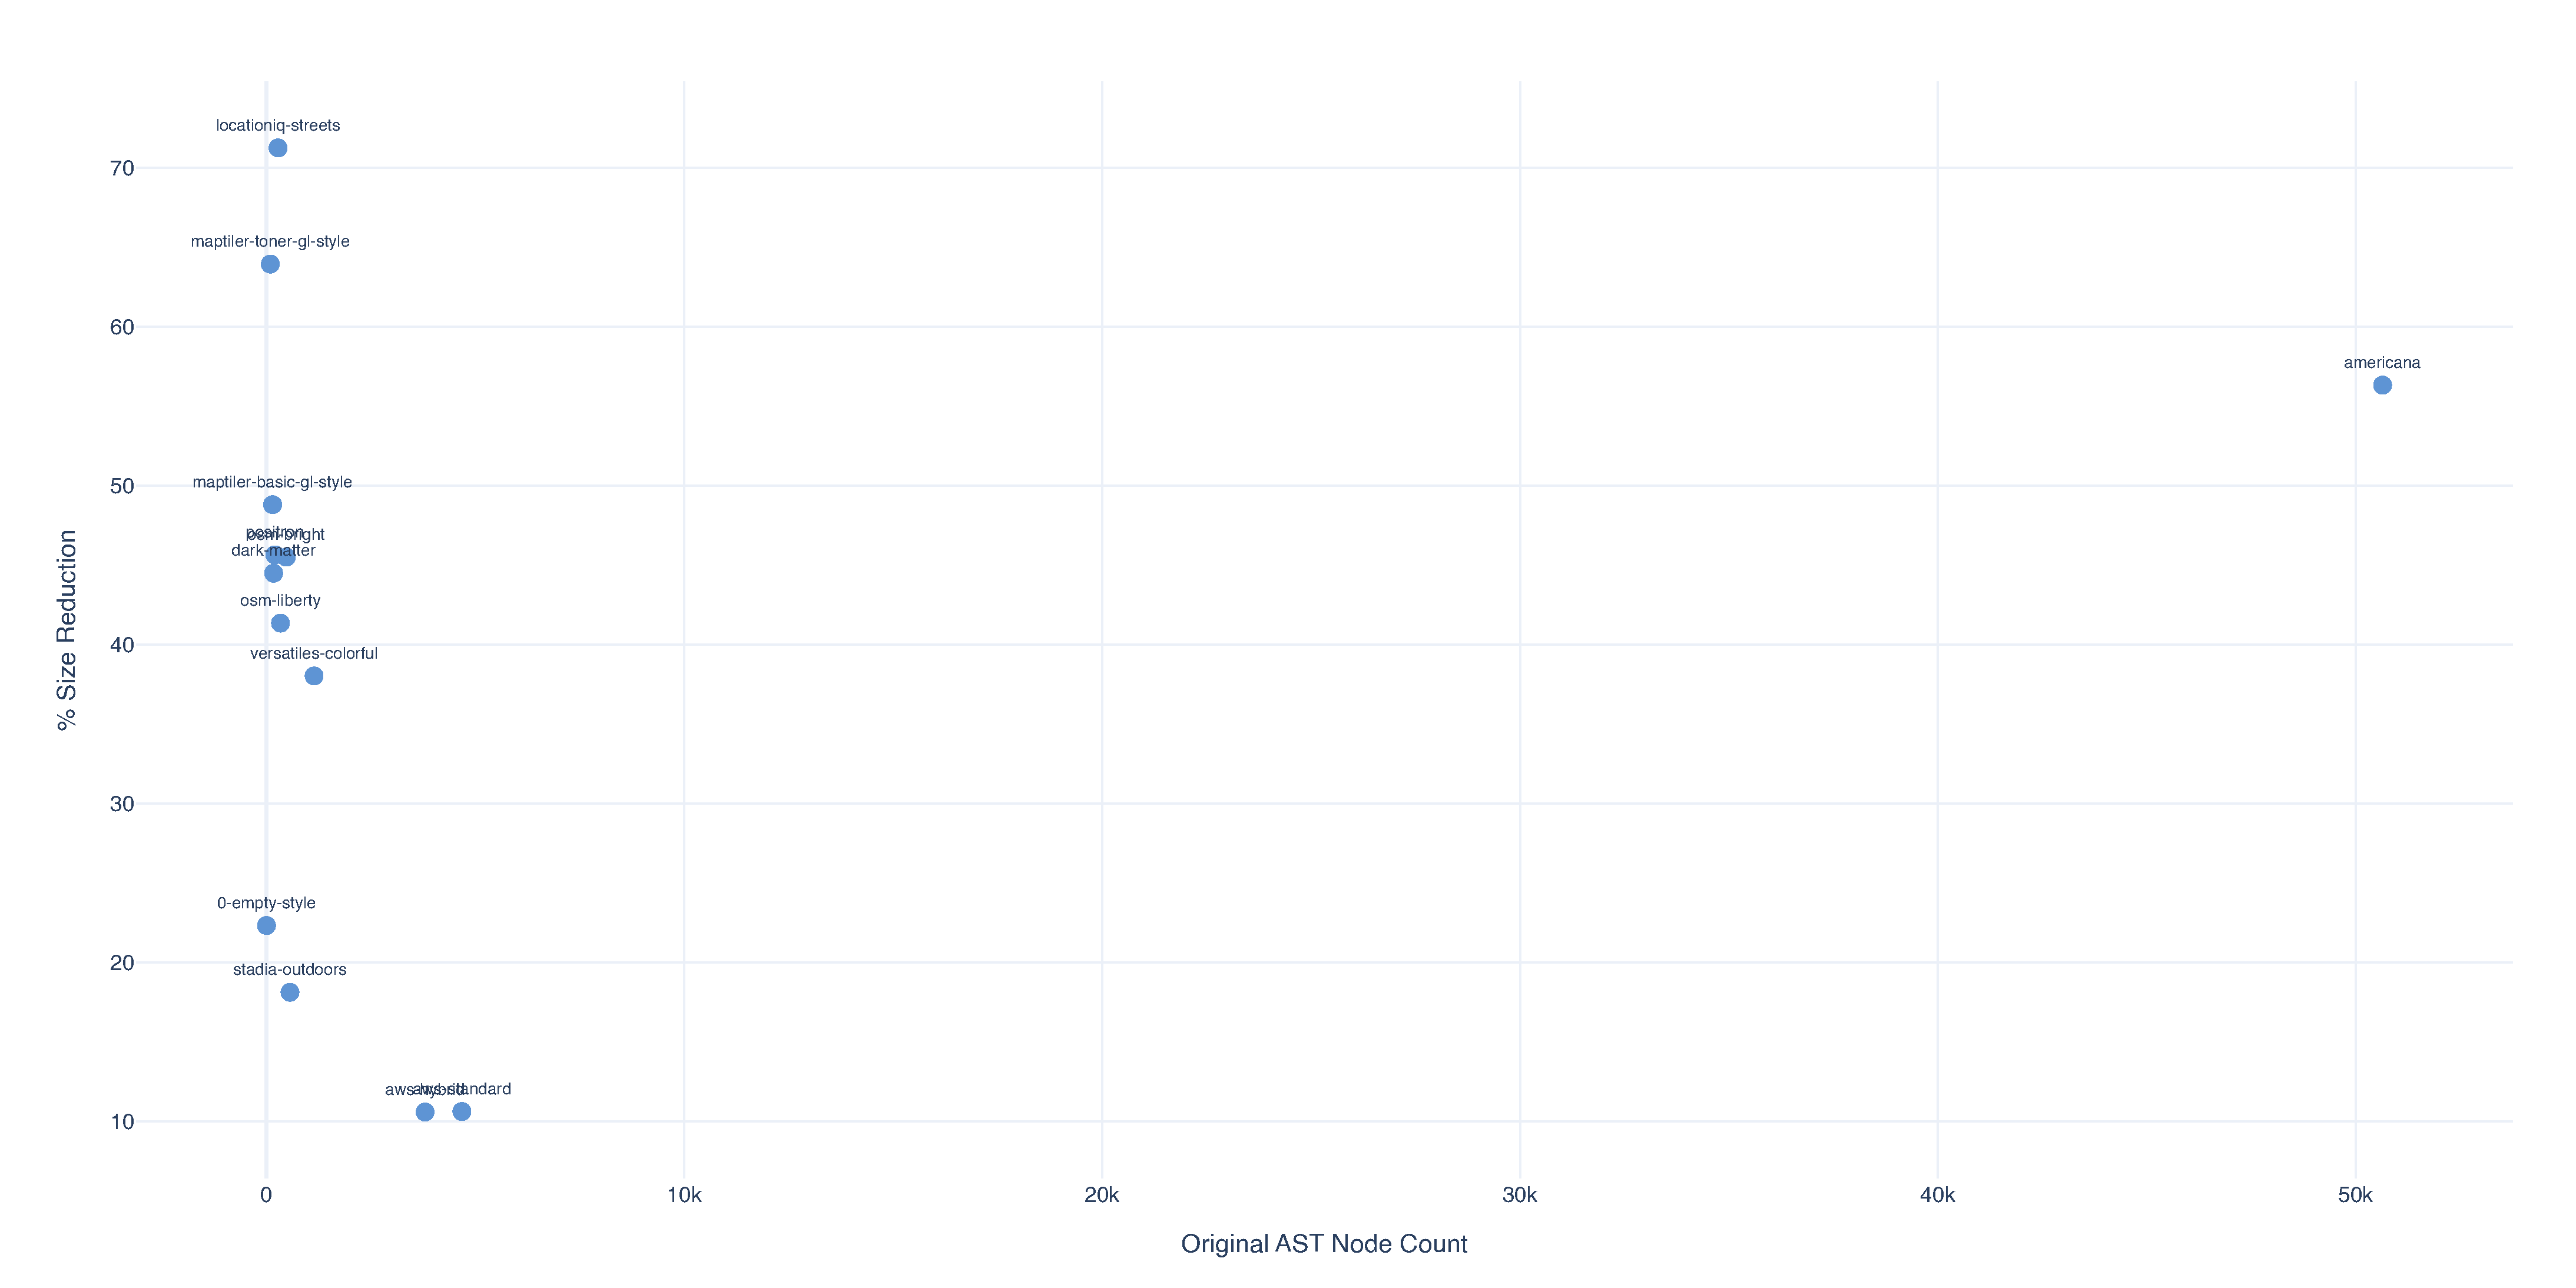
\includegraphics[width=\linewidth]{figures/cross_style_complexity_scatter.pdf}
    \caption{Relationship between initial style complexity (\ac{AST} node count) and achievable raw style size reduction across the Maputnik generalization corpus. The correlation is not statistically significant ($r = 0.35$, $n = 13$, $p = 0.24$), and is driven by a single high-leverage point (Americana); dropping it flips the sign to $r = -0.54$. Optimization yield is therefore not reliably predictable from complexity alone, but a combination of other factors such as the cartographers' skill.}
    \label{fig:cross_style_complexity_scatter}
\end{figure}

\begin{table}[htbp]
\centering
\small
\begin{tabular}{l r r r r r}
\toprule
\textbf{Metric} & \textbf{Min} & \textbf{P25} & \textbf{Median} & \textbf{P75} & \textbf{Max} \\
\midrule
Raw size reduction (\%)         &    3.2 &   22.3 &  31.4 & 38.2 & 67.7 \\
Gzip size reduction (\%)        &    3.9 &    6.0 &  11.4 & 12.2 & 22.4 \\
Brotli size reduction (\%)      &    0.7 &    3.1 &   9.8 & 11.9 & 17.0 \\
Layer count reduction (\%)      &    0.0 &    0.8 &   4.8 &  7.0 & 27.0 \\
\ac{AST} node count change (\%) & $-269.2$ & $-102.9$ & $-47.9$ & 0.0 & 62.2 \\
\bottomrule
\end{tabular}
\caption{Distribution of style-size and complexity changes across the Maputnik generalization corpus (13 styles, static passes only). Median raw reduction is \qty{31.4}{\percent} and median Brotli reduction is \qty{9.8}{\percent}. The \ac{AST}-node row is signed: positive values denote a reduction in node count, negative values denote growth from expression rewriting (e.g.\ unrolling \texttt{match} into nested \texttt{case}); only three of the 13 styles see a net node-count reduction, indicating that the byte-size gains come predominantly from style-level passes (default stripping, layer merging, metadata stripping) rather than from expression simplification alone. Source data: \texttt{scripts/data/cross\_style\_summary.csv}.}
\label{tab:cross_style_summary}
\end{table}

\subsection{Discussion}\label{sub:cross_discussion}

The static passes deliver a median raw reduction of \qty{31.4}{\percent} (range \qtyrange{3.2}{67.7}{\percent}) across the 13 unseen Maputnik styles, with no style regressing and only a weak link between initial complexity and achievable reduction ($r = 0.35$, $p = 0.24$).
We discuss which pass families generalize universally, why we read these numbers as a lower bound on the full potential, and what the low-reduction edge cases look like in practice.

\paragraph{Universality of expression passes}
Expression-level passes (constant folding, boolean simplification, default stripping) produce non-zero reductions for virtually every style in the corpus, regardless of its complexity or tile schema.
We expect this: any style written by a human or generated by an editor is likely to contain at least some redundant expressions, default-valued properties, or suboptimal color encodings.

\paragraph{Complexity and reduction}
While verbose institutional styles with several hundred layers and deeply nested expressions tend to offer more room for improvement than simple styles with fewer than 50 layers, we find that the correlation between initial style complexity and achievable reduction is not statistically significant at this sample size ($r = 0.35$, $n = 13$, $p = 0.24$), and is dominated by a single high-leverage point.
The scatter plot (\cref{fig:cross_style_complexity_scatter}) visualizes the per-style relationship.

\paragraph{Passes that require statistics are not evaluated}
Because the generalization corpus does not include tile data, we cannot apply stats-driven passes (dead elimination with geometry-type matching, stats-driven constant folding, selectivity reordering) and data-level optimizations (tile shaving, re-encoding) to the Maputnik styles.
We therefore present the reported reductions as a \emph{lower bound} on the full optimizations potential.
Extrapolating from the deep corpus, where stats-driven passes add \qtyrange{10}{20}{\percent} additional reduction on top of static passes, the true optimizations potential for these styles is likely higher.
For the 11 \ac{OMT}-compatible styles in the deep corpus, we evaluated tile shaving separately against the Germany tileset (\cref{fig:tile_shave_per_style}), confirming that data-level reductions generalize across styles.

\paragraph{Edge cases}
A small number of styles in the corpus show small reductions ($< 5\%$), the lowest being Stadia Outdoors at \qty{3.2}{\percent}.
These are typically minimal styles that already use only literal values (no expressions), have few layers, and do not set properties to their default values.
We observe no style in the corpus that shows a size \emph{increase} after optimizations, confirming that the passes are safe in the general case.
In practice, styles maintained by large organizations - which tend to accumulate verbose filters, redundant default values, and deeply nested expressions over successive authoring iterations - offer the most room for automatic simplification.
Compact basemaps authored by experienced cartographers, which already use efficient expressions and few layers, show correspondingly smaller gains.


\section{Combined Results}\label{sec:exp_combined}
\begin{keytakeaways}
\item The three optimization channels compose additively, not synergistically.
\item Data-level passes do almost nothing for sustained frame rate; their lever is load time.
\item No single pass dominates across styles - the multi-pass design is what generalizes.
\end{keytakeaways}

\noindent In this section we present the full pipeline ablation - all 19 cumulative steps from baseline through tile rewriting (and the plain-tile-shaving comparison configuration), as defined in \cref{sub:ablation} - and analyze the interactions between optimizations categories.
The combined view is essential because the three optimization categories (expression, structural, data, introduced in \cref{sub:expression_optimizations,sub:structural_optimizations,sub:data_optimizations}) can interact:
style-level dead elimination narrows tile pruning advisories, and metadata refinement enables more aggressive zoom-stop pruning in the data pipeline, though the aggregate data shows these interactions are additive rather than synergistic.

\subsection{Full Pipeline Ablation}\label{sub:combined_ablation}

\cref{fig:heatmap_loadMs} presents the full scenario$\times$step load-time heatmap.
Load-time improvements are unevenly distributed across scenarios: urban, tile-dense scenarios (New York, Tokyo, Paris) show larger absolute improvements than sparse scenarios (Sahara, Amazon), because the tile-fetch component of load time dominates in dense areas.
Expression passes (steps~1-7) produce a diffuse, moderate improvement across most scenarios, whereas the improvement from structural passes (steps~8-15) is concentrated in the few styles and scenarios where dead elimination or layer merging applies.
\cref{fig:heatmap_fps} shows the companion \ac{FPS} view: the gain is broadly aligned with the load-time pattern but lands more uniformly across scenarios, because once tiles are decoded the sustained frame rate is driven by per-feature evaluation cost rather than by tile-fetch latency.

A side effect we did not expect on first reading was that the frame-time consistency metric in \cref{fig:heatmapjankcount} \emph{got worse} as the pipeline got faster - the jank count goes up across the ablation.
The explanation, once we plotted it next to \ac{FPS}, is that we are now running well above 2000\,\ac{FPS}, where smaller variations such as \ac{GC}-pauses register as proportionally large frame-time outliers; on real consumer hardware capped well below that rate the same pauses would not cross the jank threshold.
The metric is doing what it should - flagging fragile frames - but it is reading a regime the renderer was never expected to enter, which is worth keeping in mind when interpreting the heatmap.

\begin{figure}[htbp]
	\centering
	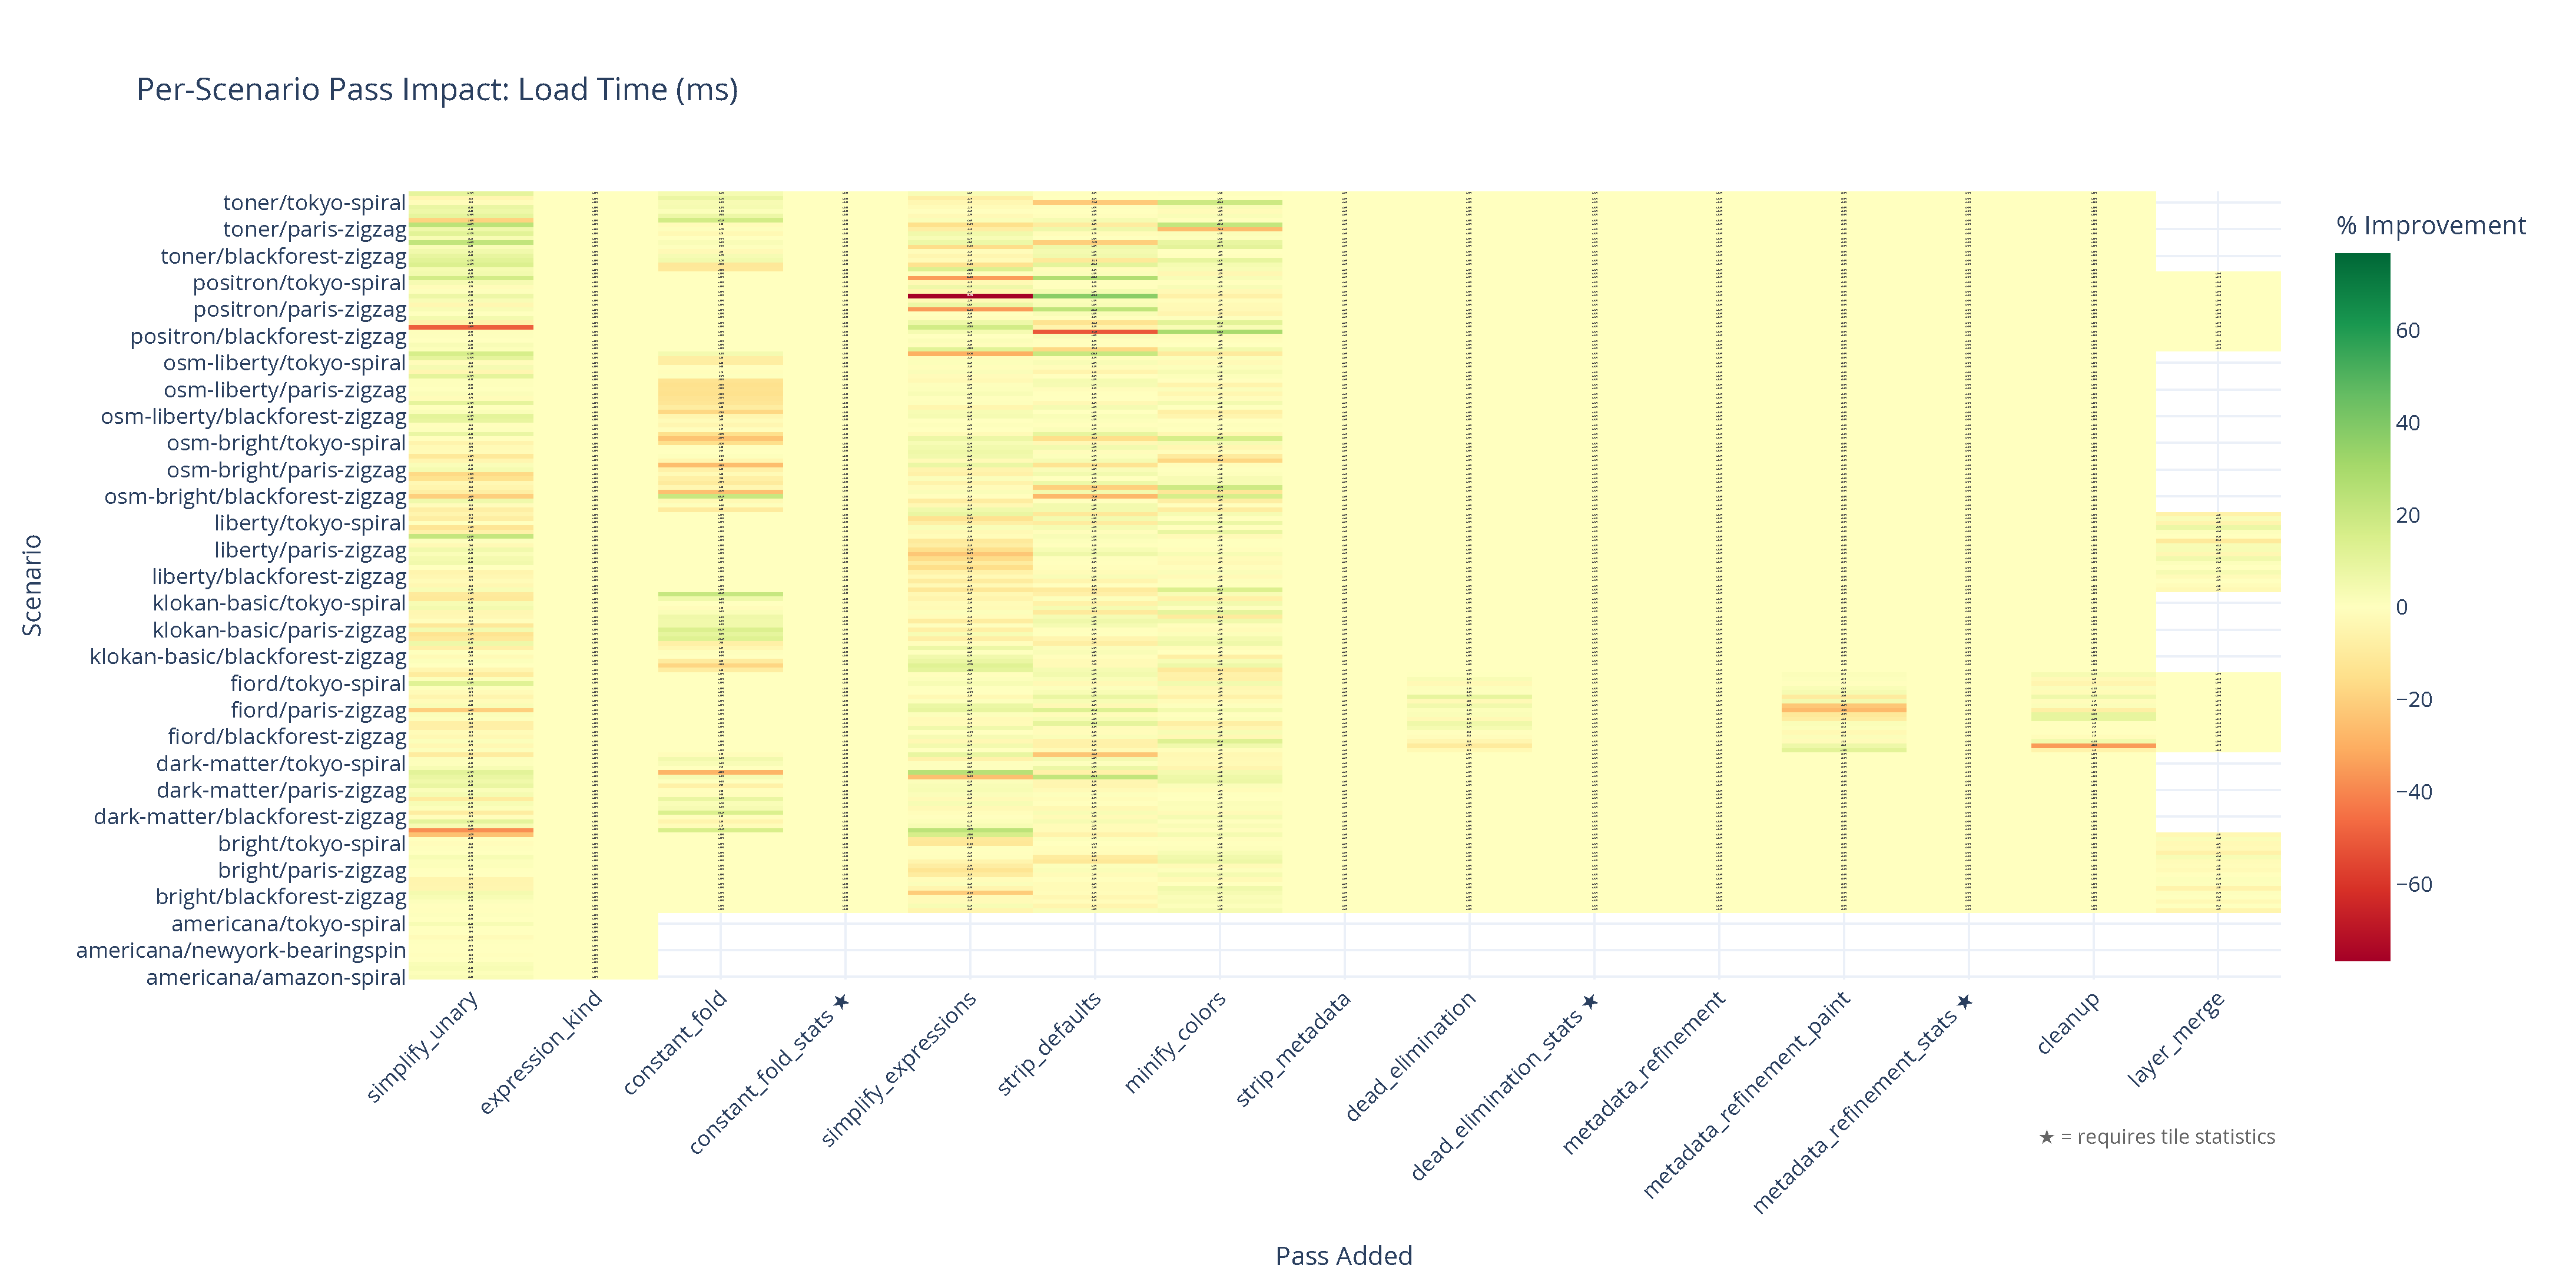
\includegraphics[height=0.9\textheight]{figures/heatmap_loadMs.pdf}
	\caption{Heatmap of load time across scenarios (rows) and ablation steps (columns); darker cells indicate greater improvement relative to baseline. Urban, tile-dense scenarios (New York, Tokyo, Paris) show the largest absolute improvements; structural passes produce concentrated gains where dead elimination or layer merging applies.}
	\label{fig:heatmap_loadMs}
\end{figure}

\begin{figure}[htbp]
	\centering
	\includegraphics[height=0.9\textheight]{figures/heatmap_fps.pdf}
	\caption{Heatmap of \ac{FPS} across scenarios (rows) and ablation steps (columns). Compared to \cref{fig:heatmap_loadMs}, the \ac{FPS} gains are distributed more uniformly across scenarios, since sustained frame rate is driven by per-feature evaluation cost rather than by tile-fetch latency once tiles are resident.}
	\label{fig:heatmap_fps}
\end{figure}

\begin{figure}[tbph]
	\centering
	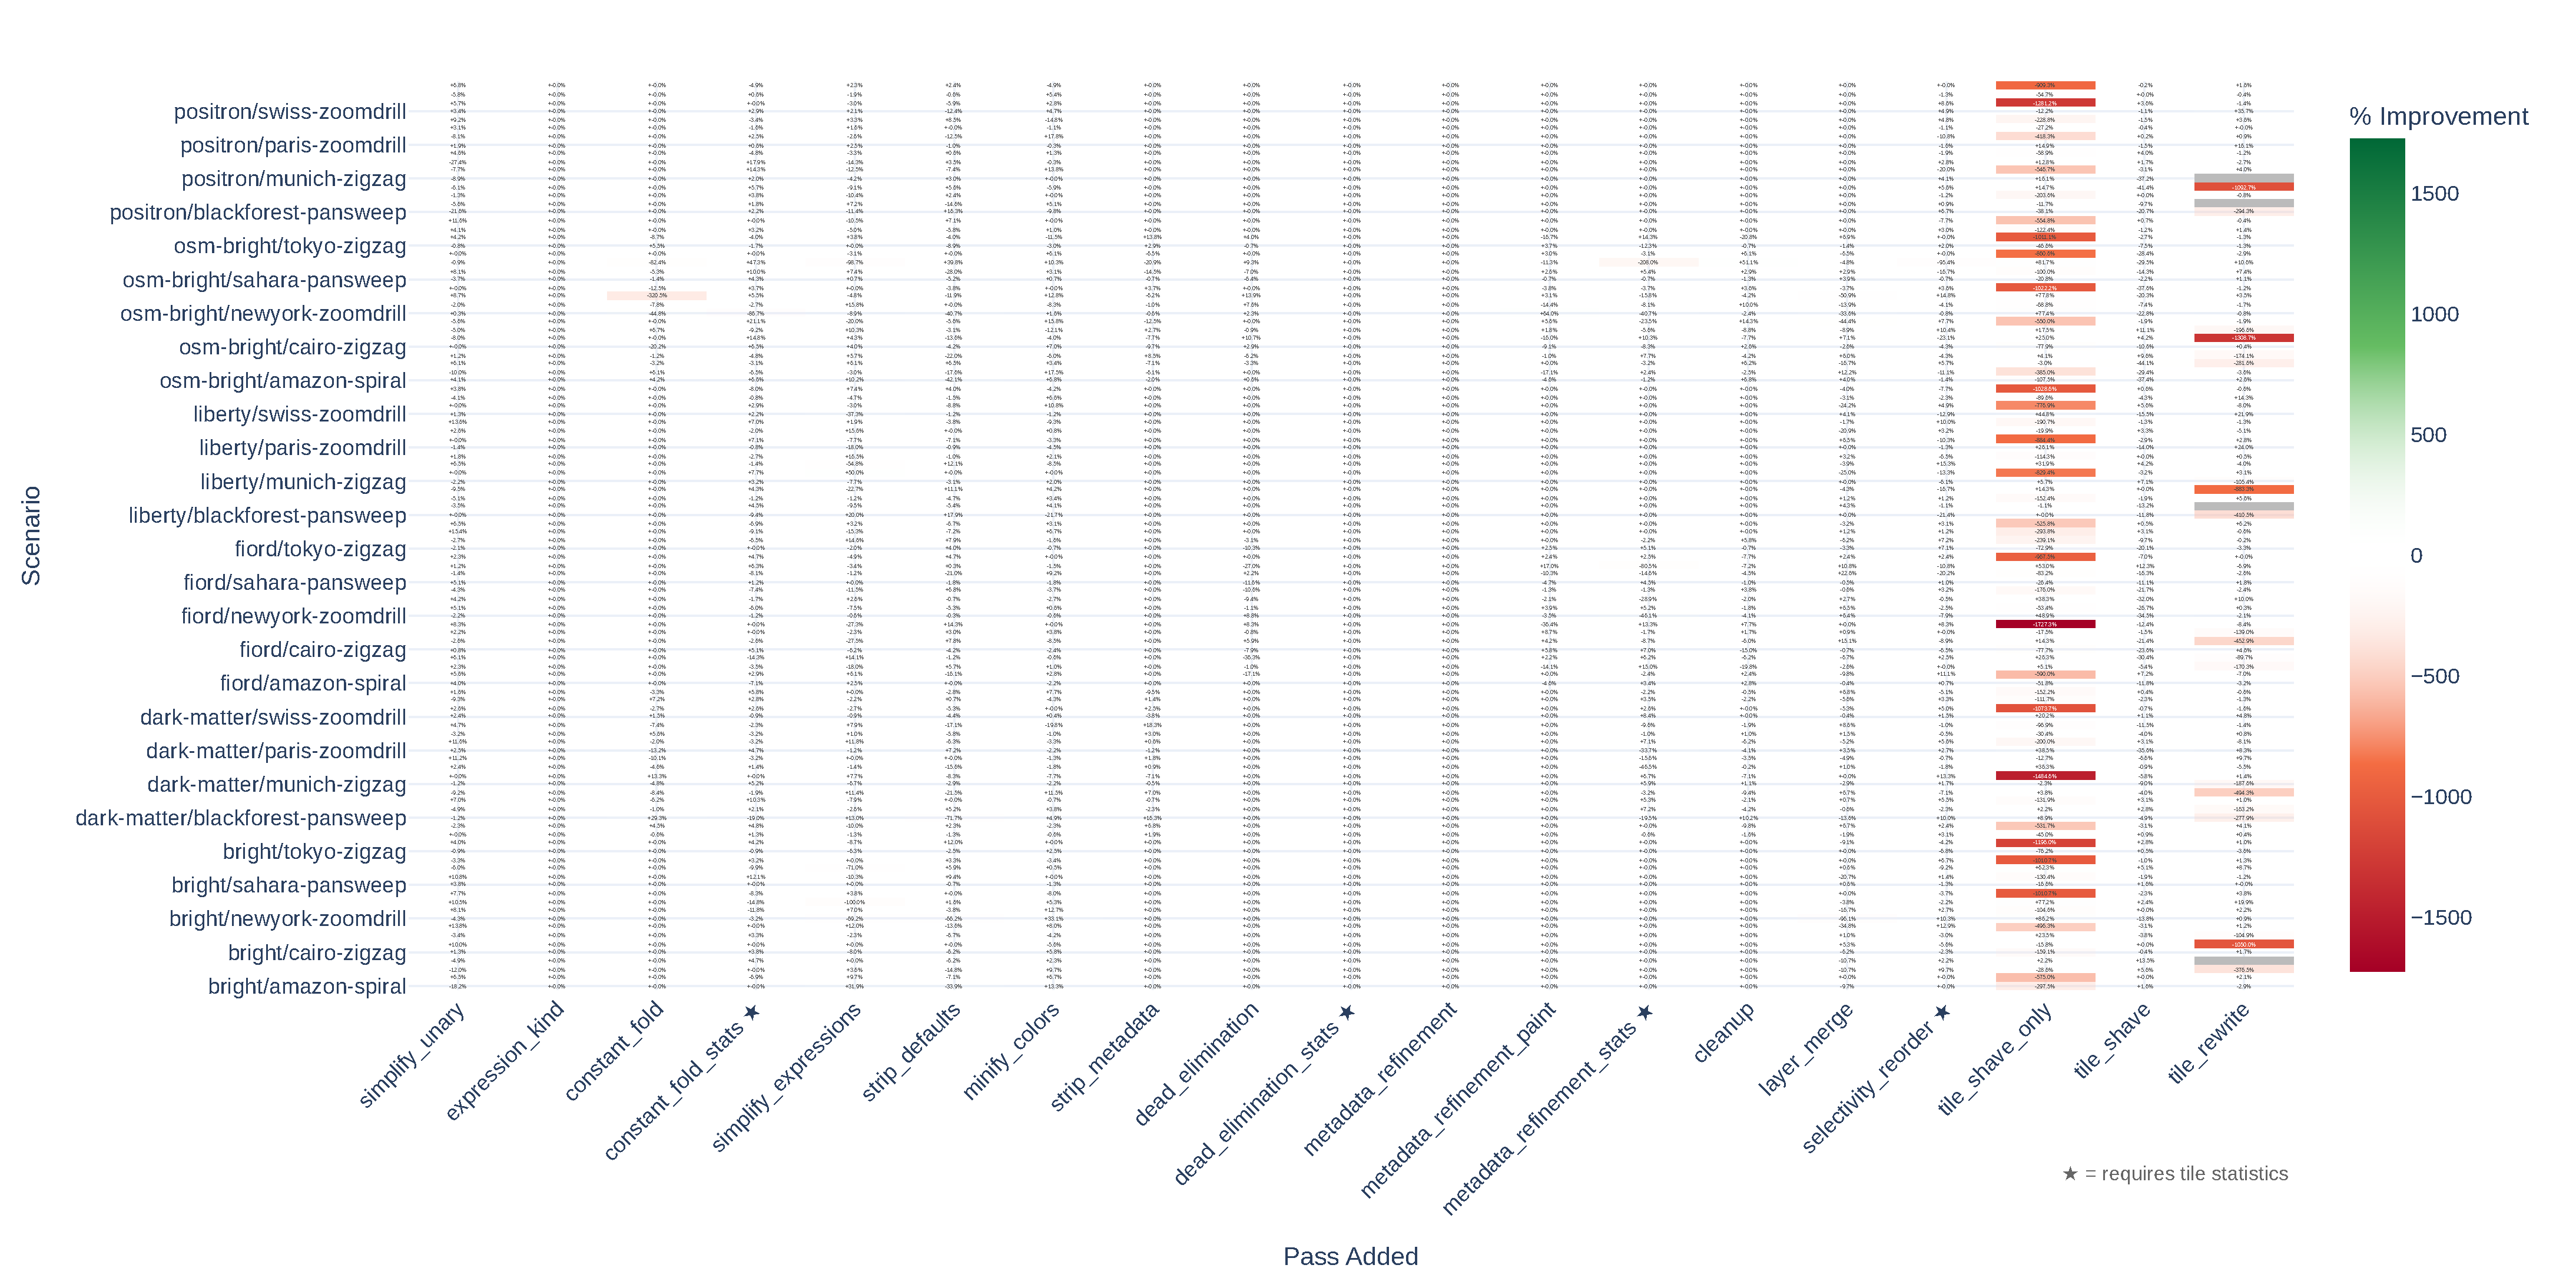
\includegraphics[height=0.9\textheight]{figures/heatmap_jankCount}
	\caption{
		Heatmap of how jank frames, i.e. frames times that are much slower than the sorrounding frame times, happen.
		Due to the increased \ac{FPS}, smaller variations like \ac{GC}-pauses make this metric go up as \ac{FPS} is higher.
		This does not nessarily have an effect to the user, since real devices render below the 2000\,\ac{FPS} marker that we run at, but nevertheless something to keep in mind.}
	\label{fig:heatmapjankcount}
\end{figure}

\cref{fig:time_breakdown} decomposes load time into its constituent phases - style parse, first tile, first frame, and remaining load - across ablation steps.
The style-parse component shrinks monotonically as the style document gets smaller, dropping from the baseline to a visibly shorter bar by step~7 (after expression passes).
The first-tile and remaining-load components are stable across style-only steps, confirming that style optimizations primarily affects parse time rather than tile-fetch time; this changes only at the tile-shaving steps (17-19), where smaller tiles reduce the first-tile phase.

\cref{fig:memory_ablation} tracks browser heap memory across steps.
Style-level passes move the resident JS heap only modestly: from the baseline mean of \qty{86.0}{\mega\byte} the heap drifts to \qty{82.9}{\mega\byte} by step~15, a total reduction of \qty{3.1}{\mega\byte} (\qty{-3.6}{\percent}), with no single style-level pass dominating.
The dominant heap reduction arrives with the data-level passes: tile shaving (step~17) alone drops the heap to \qty{63.7}{\mega\byte}, and the full pipeline through tile rewriting (step~19) reaches \qty{55.3}{\mega\byte} - a cumulative \qty{-35.7}{\percent} versus baseline, reflecting that the major heap consumer is the in-memory tile payload, not the parsed style.

\begin{figure}[htbp]
    \centering
    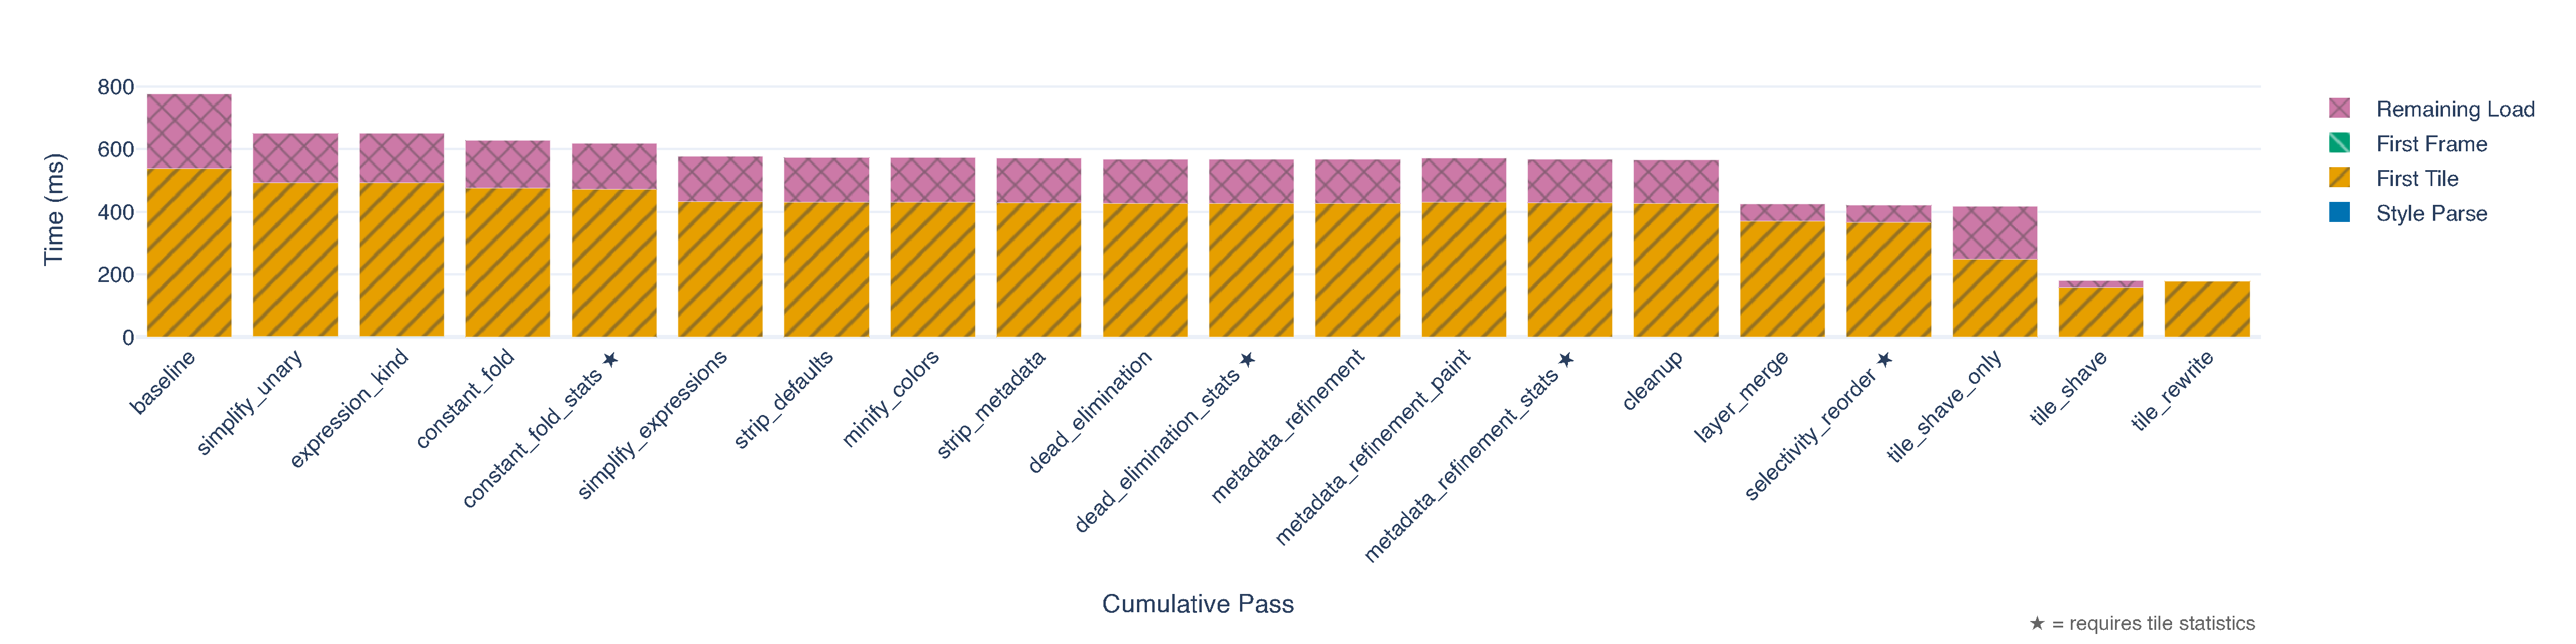
\includegraphics[width=\linewidth]{figures/time_breakdown.pdf}
    \caption{Time breakdown across ablation steps: style parse, first tile, first frame, and remaining load time. Style-parse time shrinks monotonically with each expression pass; first-tile and remaining-load times are unchanged by style-only steps and decrease only when tile shaving is applied (steps~17-19).}
    \label{fig:time_breakdown}
\end{figure}

\begin{figure}[htbp]
    \centering
    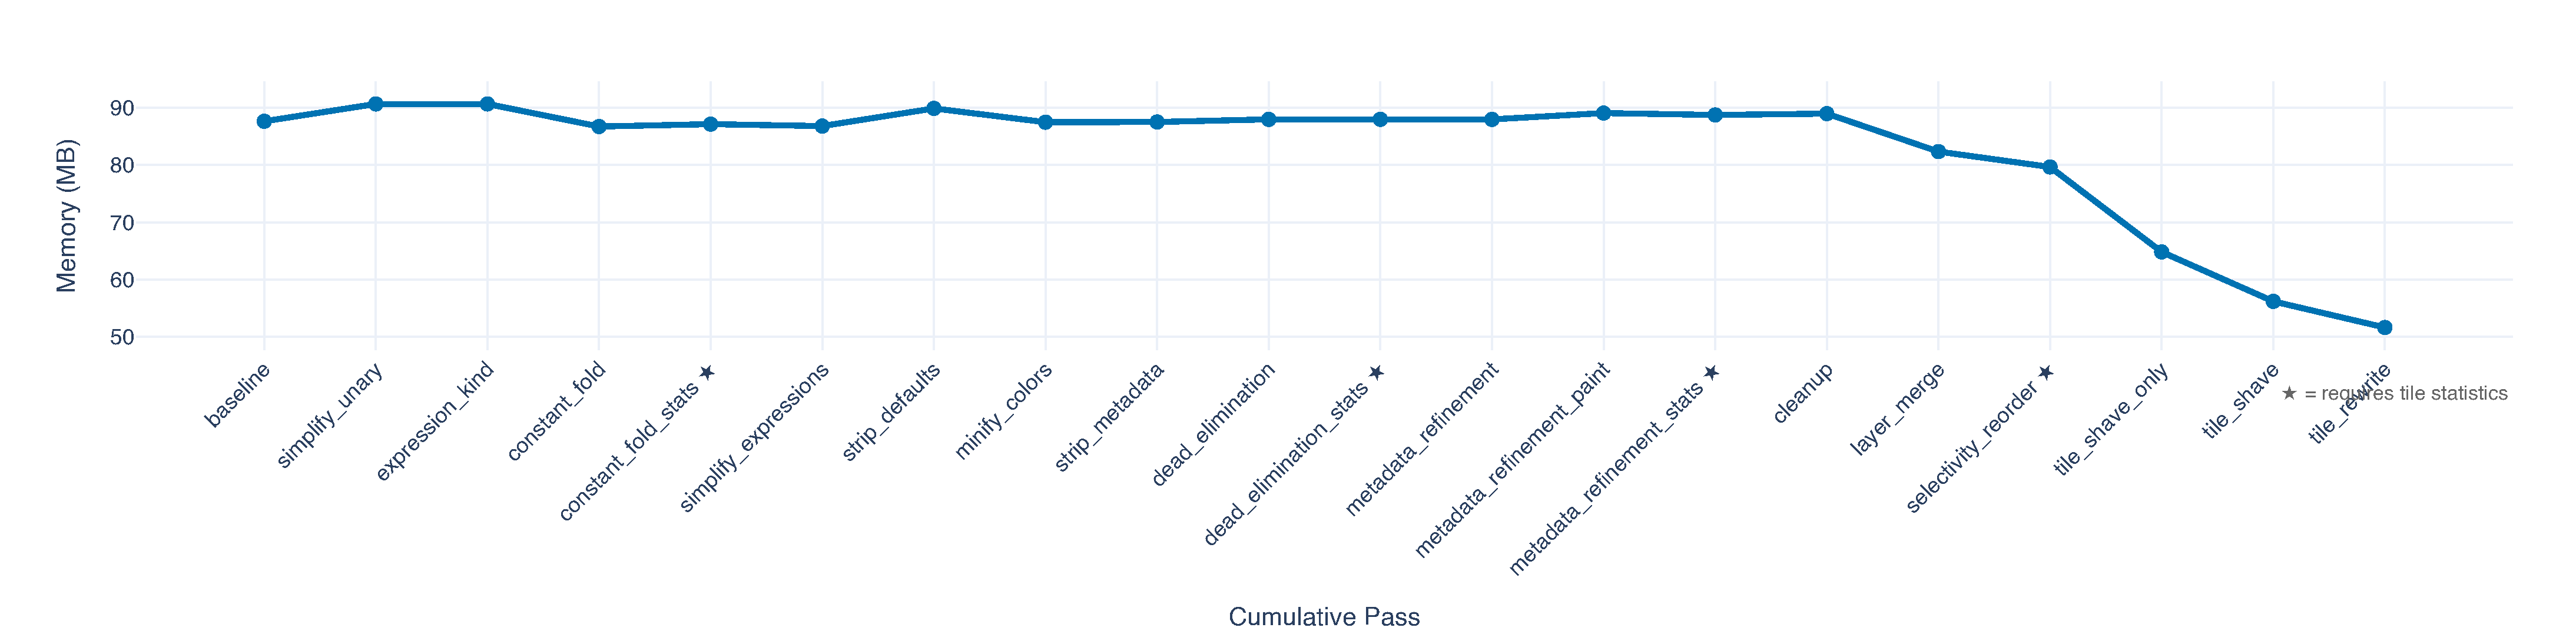
\includegraphics[width=\linewidth]{figures/memory_ablation.pdf}
    \caption{Heap memory usage (mean \texttt{heapUsedMB} across all scenarios and benchmark styles) across ablation steps. Style-level passes (steps 1-15) reduce the heap by \qty{3.1}{\mega\byte} (\qty{-3.6}{\percent}); the bulk of the heap savings comes from data-level passes (steps 17-19) where the in-memory tile payload itself shrinks, yielding a cumulative reduction of \qty{-35.7}{\percent} from baseline to step~19.}
    \label{fig:memory_ablation}
\end{figure}

\begin{table}[htbp]
\centering\small
\csvreader[
  tabular=l r r r r r,
  table head={\toprule
    \textbf{Style} & \textbf{Baseline} & \textbf{Optimised} &
    \textbf{Reduction} & \textbf{$\Delta$ Load} & \textbf{$\Delta$ FPS} \\
     & \textbf{gzip (B)} & \textbf{gzip (B)} &
     \textbf{(\%)} & \textbf{(\%)} & \textbf{(\%)} \\
    \midrule},
  table foot=\bottomrule,
  head to column names,
  before line={\ifnum\midruleBefore=1\midrule\fi},
]{scripts/data/per_style_summary.csv}{}%
{\ifnum\isBold=1\textbf{\style}\else\style\fi &
 \num{\baseGzip} & \num{\optGzip} & \reduction &
 \fmtdelta{\deltaLoad} & \fmtdelta{\deltaFps}}%
\caption{Per-style summary: baseline and optimized style size (gzip), size reduction, and change in load time and \ac{FPS} (medians across scenarios). Styles below the rule include tile-level optimizations (steps~1-19); those above include style-level optimizations only (steps~1-15). Tile shaving produces the most visible drops in load time and \ac{FPS} improvements.}
\label{tab:per_style_summary}
\end{table}

\begin{table}[htbp]
\centering
\small
\csvreader[
  tabular=r l r r r r r,
  table head={\toprule
    \textbf{Step} & \textbf{Pass} & \textbf{$\Delta$ Raw} &
    \textbf{$\Delta$ Gzip} & \textbf{$\Delta$ Brotli} &
    \textbf{$\Delta$ Load} & \textbf{$\Delta$ Layers} \\
     & & \textbf{(\%)} & \textbf{(\%)} & \textbf{(\%)} & \textbf{(\%)} & \\
    \midrule},
  table foot={\midrule
    \multicolumn{7}{l}{\footnotesize $\dagger$ Steps~16-19:
    fiord and liberty only (benchmarked with tile statistics).} \\
    \bottomrule},
  head to column names,
]{scripts/data/marginal_contribution.csv}{}%
{\step & \pass\ifnum\dagger=1\textsuperscript{$\dagger$}\fi &
 \fmtdelta{\deltaRaw} & \fmtdelta{\deltaGzip} & \fmtdelta{\deltaBrotli} &
 \fmtdelta{\deltaLoad} & \fmtdeltaint{\deltaLayers}}%
\caption{Marginal contribution of each ablation step to style size (raw, gzip, Brotli), load time, and layer count; values are percentage of baseline, medians across 12 styles and 18 scenarios. Data-level tile shaving dominates transfer-size and load-time metrics; style-level passes contribute primarily to parse-time and style-size reductions and serve as enablers for the data-level pipeline.}
\label{tab:marginal_contribution}
\end{table}

\subsection{Marginal Contribution Analysis}\label{sub:combined_marginal}

Not all passes contribute equally, and the marginal contribution of each pass depends on the metric under consideration.

\paragraph{Rendering time metrics}
After tile shaving, we observe that expression-level constant folding and structural dead elimination tend to produce the largest marginal improvements in frame time and \ac{FPS}, as they reduce the number of expressions the renderer must evaluate per feature per frame and the number of layers it must process, respectively.
Layer merging produces a large marginal improvement in draw-call-heavy styles (many road layers, many boundary layers) but a smaller improvement in simple styles.

\paragraph{Transfer size metrics}
Passes that primarily reduce serialized style size - default stripping, metadata stripping, color minification - show smaller rendering improvements but contribute meaningfully to transfer size, particularly under compression (gzip, Brotli).
A smaller style reduces the time to first render because the \ac{JSON} must be fetched, decompressed, and parsed before the renderer can initialise.
Data-level tile shaving dominates the transfer-size metric, as tiles are fetched continuously during map interaction whereas the style is loaded only once.

\paragraph{Load time metrics}
Both style size (initial fetch and parse) and tile size (first tile fetch) influence load time.
Style-level passes improve style parse time; data-level passes improve first-tile time.
The relative contribution depends on the network bandwidth: under the \qty{10}{\Mbps} throttle, tile-fetch latency dominates; under the \qty{1.5}{\Mbps} throttle, style-fetch latency becomes significant for large styles.

\subsection{Preprocessing Cost}\label{sub:preprocessing_cost}

Research Goal~R3 asks how expensive the optimizations are in terms of preprocessing time.
The optimizations pipeline is an \emph{offline} stage: we optimize a style once and serve it many times, and re-encode tiles once per tileset build.
Preprocessing cost is therefore amortised over all subsequent tile deliveries and is not on the user's critical path, but it still matters for operational feasibility on large tilesets.

In this section we measure each of the four additive cost terms $C_\text{style}$, $C_\text{stats}$, $C_\text{adv}$, and $C_\text{enc}$ from the preprocessing cost model (\cref{eq:cost_model}, \cref{sub:preprocessing_cost_model}) on a real tileset, and confirm that the cost-control mechanisms formalised there keep the multi-strategy overhead well below the na\"ive worst case.

\paragraph{Measured stage costs}
\Cref{tab:preprocessing_cost} reports wall-clock time for each stage of the preprocessing pipeline on the Germany OpenMapTiles tileset (\num{256156} tiles after pruning, zoom 0-14), which we measured on an AMD Ryzen~7 3700X (8 cores / 16 threads), \qty{46}{\gibi\byte} \ac{RAM}, NVMe SSD; median of three runs.
\emph{Style optimization} ($C_\text{style}$) and \emph{advisory computation} ($C_\text{adv}$) are negligible: Liberty's 111-layer style completes all passes in \qty{7.5}{\milli\second} and the advisory in \qty{1.1}{\milli\second}.
\emph{Tile-statistics collection} ($C_\text{stats}$) takes \qty{57.4}{\second} for a single-threaded scan of all \num{256588} source tiles.
\emph{Tile pruning and \ac{MVT} re-encoding} ($C_\text{enc}$, MVT) takes \qty{15.6}{\second} using Rayon\footnote{\url{https://github.com/rayon-rs/rayon}, last accessed 2026-05-23} parallelism.
\emph{\ac{MLT} encoding with sort-strategy competition} ($C_\text{enc}$, \ac{MLT} auto) is the dominant term: \qty{5}{\minute}\,\qty{42}{\second} single-threaded, or \qty{47}{\second} with 16 threads.
Without the competition ($C_\text{enc}$, \ac{MLT} none), single-threaded encoding takes \qty{2}{\minute}\,\qty{55}{\second}.
We therefore measure the overhead ratio of the full competition at $342 / 175 = 1.95\times$ in \ac{CPU} time - substantially lower than the analytical 3-5$\times$ estimate, because the cost-control mechanisms formalised in \cref{sub:preprocessing_cost_model} eliminate most redundant work.

\begin{table}[htbp]
\centering\small
\begin{tabular}{l l r}
\textbf{Stage} & \textbf{Description} & \textbf{Wall-clock} \\
\midrule
$C_\text{style}$ & Style optimization (all passes, Liberty) & \qty{7.5}{\milli\second} \\
$C_\text{stats}$ & Tile statistics (\num{256588} tiles, 1 thread) & \qty{57.4}{\second} \\
$C_\text{adv}$ & Advisory computation & \qty{1.1}{\milli\second} \\
$C_\text{enc}$ (\ac{MVT} prune) & Tile pruning + \ac{MVT} re-encode (16 threads) & \qty{15.6}{\second} \\
$C_\text{enc}$ (\ac{MLT} none, 1T) & \ac{MLT} encoding, single strategy, 1 thread & \qty{175}{\second} \\
$C_\text{enc}$ (\ac{MLT} auto, 1T) & \ac{MLT} encoding, full competition, 1 thread & \qty{342}{\second} \\
$C_\text{enc}$ (\ac{MLT} auto, 16T) & \ac{MLT} encoding, full competition, 16 threads & \qty{46.7}{\second} \\
\midrule
Overhead factor & auto\,/\,none (single-threaded CPU time) & $1.95\times$ \\
\end{tabular}
\caption{Preprocessing wall-clock time per pipeline stage on the Germany OpenMapTiles tileset (zoom 0-14, \num{256156} tiles after pruning) when run on \cref{tab:bench_hardware}. Median of 3~runs. Style optimization ($C_\text{style}$, \qty{7.5}{\milli\second}) and advisory computation ($C_\text{adv}$, \qty{1.1}{\milli\second}) are negligible; \ac{MLT} encoding with full sort-strategy competition dominates at \qty{342}{\second} single-threaded (\qty{46.7}{\second} with 16 threads), with an overhead factor of $1.95\times$ vs.\ a fixed-plan encoder.}
\label{tab:preprocessing_cost}
\end{table}

\paragraph{Amortisation and headline numbers}
Taken together, the cost-control mechanisms formalised in \cref{sub:preprocessing_cost_model} - bounding-box pruning, data profiling, warm-start caching, scratch-buffer recycling, and the \ac{RAII} alternatives guard - reduce the measured overhead of the full sort-strategy competition to $1.95\times$ compared to a fixed-plan (single-strategy) encoder (\cref{tab:preprocessing_cost}), well below the na\"ive $4\times$ expectation from four candidate sort orders.
We empirically confirm that the trial-and-retain loop costs $k$ encode passes plus $\mathcal{O}(1)$ bookkeeping rather than $k$ encode passes plus $k$ full buffer clones.
We pay this cost once per tileset build and amortise it over every subsequent tile request.
The total single-threaded pipeline time (statistics collection through \ac{MLT} encoding with full competition) is under \qty{7}{\minute} on the Germany tileset; with 16-thread parallelism the end-to-end wall-clock time drops to approximately \qty{2}{\minute} - perfectly acceptable for an offline build stage.
The effect of this on client side performance is not as big as it could currently be, because internally we transform data to \acsp{MVT} instead of a more efficient in-memory-structure.

\subsection{Complexity Metrics}\label{sub:combined_complexity}

The four complexity metrics we track across ablation steps (\cref{sub:metrics}) give a structural explanation for the observed rendering improvements:
expression passes (constant folding, simplification) drive the largest reductions in \ac{AST} node count;
boolean flattening and De~Morgan rewrites drive the maximum-depth reductions;
dead elimination and layer merging drive the layer-count reductions; and
metadata refinement (by consuming zoom predicates) together with dead elimination drive the filter-count reductions.
Where the same step appears across two complexity axes, we describe the connection to the corresponding rendering metric in \cref{sub:combined_marginal}.

\subsection{Discussion}\label{sub:combined_discussion}

Composed end-to-end across the ten deep-corpus styles, the full pipeline cuts per-style median load time by \qty{71}{\percent} and lifts \ac{FPS} by \qty{152}{\percent}; the three optimization channels (expression, structural, data) compose additively, not synergistically.
The following paragraphs decompose which cost channel each family acts on, separate the load-time levers from the frame-rate levers, and close with the measurement-noise caveats that bound these headline numbers.

\paragraph{Three plausible improvement channels}
The full pipeline ablation points to three plausible channels by which the optimizer improves rendering performance, which we infer from proxy metrics (\ac{AST} node count, layer count, tile size) rather than direct per-mechanism instrumentation.
The expression passes (\cref{sub:expression_optimizations}) plausibly reduce per-feature evaluation cost - fewer \ac{AST} nodes mean fewer interpreter steps per feature per frame.
Dead elimination and layer merging (\cref{sub:structural_optimizations}) operate one level up, cutting draw calls, \ac{GPU} state changes, and per-layer filter evaluations.
Tile shaving and re-encoding (\cref{sub:data_optimizations}) sit on a different axis entirely: they reduce transfer and decode cost so that load time and time-to-first-tile drop, with a secondary effect on average frame time via lower \ac{GC}-spend.
No renderer instrumentation separates these channels directly; the decomposition is inferred from the proxy metrics and the time breakdown (\cref{fig:time_breakdown}).
What makes them additive in the aggregate (as already shown quantitatively in \cref{sub:mlt_results}) is that they target non-overlapping costs: simplification cannot shrink tiles, shaving cannot prune expressions.

\paragraph{Load time vs.\ frame rate}
Expression and structural passes improve both load time and frame rate, because a simpler style is both faster to parse and faster to render.
Data-level passes primarily improve load time (smaller tiles arrive faster) and have a smaller effect on sustained frame rate, since once tiles are decoded and resident in the \ac{GPU} the per-frame cost is dominated by expression evaluation and draw-call overhead rather than data size.
The exception is tile shaving at overview zoom levels, where removing entire source-layers reduces the number of features the renderer must process per frame.

\paragraph{What varies, and why}
The cumulative ablation shows diminishing marginal returns:
early passes (constant folding, dead elimination) capture the largest improvements because they address the most common sources of waste, while later passes (color minification, metadata stripping) address less frequent patterns and contribute correspondingly less.
The non-cumulative isolated-impact analysis confirms that each pass has a non-trivial standalone contribution, even when its cumulative-sequence contribution looks small - the marginal number is sensitive to which passes precede it, but the standalone number is not.

Variation across styles is similarly structured:
styles with many narrowly-filtered layers (e.g.\ detailed road styles) benefit most from layer merging, styles with broad filters from stats-driven dead elimination, and styles with large expression trees from constant folding.
No single pass dominates across all styles, which is the empirical justification for the multi-pass design.

\paragraph{Measurement noise}
The 15-run median smooths out most measurement noise, but tail metrics (p99 frame time, jank count) carry higher variance than central-tendency metrics; \ac{GPU} thermals, browser garbage collection, and OS scheduling all contribute.
We partly self-inflict this: using real \ac{GPU} hardware (ANGLE/Vulkan) rather than a software rasteriser captures realistic rendering costs - \ac{GPU} buffer management, shader compilation - at the expense of slightly higher noise compared to deterministic software rendering.


\section{Visual Correctness Validation}\label{sec:visual_correctness}

We verified visual losslessness (\cref{eq:visual_equivalence}, with the per-pass soundness arguments collected in \cref{sec:building_optimizations}) with pixelmatch\footnote{\url{https://github.com/mapbox/pixelmatch}, last accessed 2026-05-23} across all 15 benchmark styles at zoom levels~0-14, across all 18 scenarios from \cref{sub:scenarios}, in both axis-aligned and pitched views, at \texttt{pixelRatio}~1 and using MapLibre GL~JS's Node-side software rasteriser.
Across every comparison, the fraction of differing pixels stayed below pixelmatch's per-test tolerance (default \texttt{allowed}~$=0.00025$ at the YIQ-perceptual \texttt{threshold}~$=0.1285$), confirming that every optimizations pass preserves visual identity on the software rasteriser within the perceptual-difference budget used by the upstream MapLibre render harness.

\section{Threats to Validity}\label{sec:threats}

In this section we discuss potential threats to the validity of the experimental findings.

\paragraph{Internal validity}
We conducted all rendering benchmarks on a single hardware configuration (\ac{GPU} model, \ac{CPU}, memory) running a specific browser version with ANGLE/Vulkan as the graphics backend; the full host, driver, toolchain, and dependency dump is in \cref{app:bench_env}.
Performance characteristics may differ on other hardware or with different graphics backends (e.g., native OpenGL, DirectX, Metal).
We chose the 15-run median to reduce measurement noise, but rare performance events (e.g., \ac{GPU} thermal throttling, garbage collection pauses) may not be fully captured.
The caching proxy eliminates network variability but also prevents observation of real-world caching effects and \ac{CDN} behavior.

\paragraph{External validity}
We limit the evaluation to MapLibre GL~JS.
Results may not transfer directly to other renderers such as Mapbox GL~JS, deck.gl, or native MapLibre implementations.
The tile data uses only OpenMapTiles and BasemapDE schemas. Other schemas with different property distributions or geometry characteristics may yield different optimizations gains.
The 15 benchmark styles, while diverse, may not represent all style authoring patterns encountered in production deployments.

\paragraph{End-to-end data-level coverage}
We benchmark the full rendering pipeline - style optimizations through tile shaving to \ac{MLT} re-encoding - end-to-end on 10 of the 15 deep-corpus styles (bright, dark-matter, fiord, klokan-basic, liberty, osm-bright, osm-liberty, positron, stadia-outdoors, toner).
ICGC Fosc and ICGC Gris were excluded because the legacy \mlprop{\texttt{text-field}} handling described in \cref{sub:deep_corpus} renders incorrectly under MapLibre's silent migration; the BasemapDE pair was excluded because its tile source is not \ac{OMT}-compatible and we could not provision matching shaved tiles.
For the remaining \ac{OMT}-compatible deep-corpus styles we verified the tile-shaving step alone (advisory generation and \ac{MVT} pruning, without rendering) on the same Germany tileset (\cref{fig:tile_shave_per_style}), confirming that shaving effectiveness generalizes across styles with reductions of \qtyrange{19.8}{46.3}{\percent}.
The remaining limitation is that tile statistics at a sample rate of~1.0 require access to the underlying tile data, which is available only for \ac{OSM}-based tilesets accessed via a local \texttt{.mbtiles} file.
The style-only results (Experiments~1-2) cover all 15 styles and are not affected by this limitation.

\paragraph{Construct validity}
We simulate network conditions via a fixed bandwidth throttle (\cref{sub:tile_data}) rather than measuring under real \ac{CDN} latency profiles.
We designed the synthetic camera animations of \cref{sub:scenarios} (zigzag, spiral, zoomdrill, pansweep, bearingspin) to exercise diverse rendering workloads, but they may not capture typical user interaction patterns such as search-and-zoom workflows.

\paragraph{Statistical validity}
The tile statistics (\cref{sub:tile_statistics}) count feature \emph{occurrences} across tiles, not unique geographic entities: a highway spanning 50 tiles is counted 50 times.
This inflates total feature counts and distorts absolute selectivity estimates, though relative selectivity ordering (which is all the reordering heuristic of \cref{sec:selectivity_reordering} consumes) is less affected.
We made this choice deliberatiley because the underlying features are not a concearn for the renderer on most layers (exception being symbol placement which is map-global instead of tile-local).

The selectivity estimation model assumes independence between filter predicates (\cref{eq:selectivity_compound}), which may not hold for correlated properties; map-style filters in practice do exhibit correlations (e.g.\ \mlval{\texttt{class}} and \mlval{\texttt{subclass}} in OpenMapTiles), so we treat the estimator as a first-order approximation rather than a calibrated model, and we understand selectivity-based reordering as a heuristic that produces a locally-good ordering rather than a provably-optimal one.

The 15-run median provides robustness against outliers but does not quantify sampling uncertainty on its own.
We computed bootstrap \qty{95}{\percent} confidence intervals~\cite{efronIntroductionBootstrap1998} (10\,000 resamples, percentile method) over the per-(style, variant) measurement pools for \texttt{loadMs} and \texttt{fps}.
Error bars in the waterfall (\cref{fig:waterfall_loadMs}), and rendering-metrics (\cref{fig:rendering_metrics_mlt}) figures represent these bootstrap \qty{95}{\percent} CIs.
Wilcoxon signed-rank tests (or Mann-Whitney~U where sample sizes differ) confirm that the full-pipeline load-time reductions are highly significant for both end-to-end styles (Fiord: \qty{370.9}{\milli\second}$\to$\qty{120.5}{\milli\second}, $p < 10^{-45}$, $n = 270$; Liberty: \qty{466.5}{\milli\second}$\to$\qty{133.7}{\milli\second}, $p < 10^{-74}$, $n = 254$; Fiord's pool covers all 18 scenarios $\times$ 15 runs, Liberty's full-pipeline pool covers 17 of 18 scenarios -- one scenario was absent from the pipeline output and one scenario contributed 14 of 15 runs).
Because the 18 scenarios share hardware, tile data, and styles, they are not fully independent observations; the effective sample size is smaller than $n = 270$, and we interpret the reported $p$-values as descriptive evidence of large effect sizes rather than as strict inferential tests.

Style-only effects on load time are smaller and, for individual styles, not consistently distinguishable from measurement noise.

The cumulative ablation design (\cref{sub:ablation}) means that the reported marginal contribution of each pass depends on the ordering of preceding passes; a leave-one-out or fractional-factorial design would isolate each pass's standalone contribution more cleanly but we did not run it for cost reasons.

Tail metrics (p99 frame time, jank count) are particularly sensitive to sample size: with $n=15$ runs, the tail carries only a handful of informative samples per cell, and the reported numbers should be read as directional rather than conclusive.
The full-pipeline ablation performs thousands of pairwise comparisons across metrics, styles, scenarios, and ablation steps; we apply no multiple-comparisons correction (Bonferroni, Benjamini-Hochberg), so individual per-cell \enquote{significant} differences should not be read as hypothesis tests, only as descriptive summaries.

\begin{chaptersummary}
Each pass family behaves differently in isolation: expression passes barely move load time on their own but enable the downstream passes; the structural family's gains come almost entirely from dead-layer elimination and layer merging; and on the data side, \textbf{tile shaving dominates} with a \qty{-71.5}{\percent} \textbf{median load reduction}, while the \ac{MLT} encoder's per-stream strategy competition - not the format itself - delivers a further \qty{28}{\percent} tile-volume cut over the Java reference (\qty{12}{\percent} over gzip-compressed \ac{MVT}).
Composed end-to-end across the ten deep-corpus styles benchmarked with tile data, the full pipeline reduces load time by \qtyrange{63}{74}{\percent} (per-style median \qty{71}{\percent}) and improves \ac{FPS} by \qtyrange{100}{200}{\percent} (per-style median \qty{152}{\percent}), but the cross-family interaction is \textbf{additive rather than synergistic}; the pooled Fiord+Liberty aggregate used in the \ac{MLT} discussion (\qty{+176}{\percent}) is a different aggregation of the same data restricted to the two end-to-end styles, not a conflicting headline.
The static passes generalize: a \textbf{median \qty{31.4}{\percent} raw style reduction across 13 unseen styles}, with none regressed.

The following chapter consolidates these findings into architectural claims, answers the research questions of \cref{sec:research_goals}, and identifies the directions left open.
\end{chaptersummary}

\chapter{Conclusion}\label{ch:conclusion}

In the preceding chapter we evaluated each optimisation level in isolation and then measured their combined effect, revealing that tile shaving and columnar re-encoding dominate the load-time improvements while style-level passes provide modest, additive contributions.
In this chapter we draw together the findings: we summarise our contributions, distil the key insights, revisit the three research questions posed in \cref{sec:research_goals}, and identify directions for future work.

\section{Summary of Contributions}

Our main contributions are:

\begin{enumerate}
    \item We present a \textbf{three-level optimisation pipeline} (\cref{sub:pipeline}) that proved most effective as an enabler: expression-level simplifications cascaded into forms that structural passes could exploit, with constant folding and dead elimination together accounting for the largest per-pass rendering gains (\cref{sub:combined_marginal}).
    We observed that some passes, such as the default removal passes, had both positive and negative effects on the metrics measured, but not to a significant enough extent to alter the overall trend.

    \item We show that \textbf{style-driven tile shaving} (\cref{sub:tile_shaving}) is the dominant contributor to load-time and transfer-size improvements.  Dead elimination narrows the pruning advisory, enabling elimination of property columns and tiles from the encoded output, though we find the interaction with style-level passes to be additive rather than synergistic (\cref{sub:mlt_discussion}).

    \item We contribute \textbf{automatic encoding strategy selection} for the \ac{MLT} format, which closed the gap that the fixed-plan Java encoder left open: the Rust encoder's per-stream profiling and sort-strategy competition reduced tile volume by \qty{28}{\percent} over the Java baseline, and we found this advantage to persist under every wire compressor tested (\cref{tab:mvt_mlt_comparison}).

    \item Through our \textbf{empirical evaluation} (\cref{ch:experiments}) we confirm that the three optimisation categories are complementary: expression and structural passes dominate rendering-throughput improvements, while data-level passes dominate load-time improvements, with the full pipeline reducing total tile volume by \qty{28}{\percent} (\qty{12}{\percent} over gzip-compressed \ac{MVT}) and improving end-to-end load times by \qtyrange{71}{75}{\percent} on the two styles we benchmarked with tile data.
\end{enumerate}

\section{Key Findings}

From our evaluation we draw three architectural insights that go beyond the quantitative results we report in \cref{ch:experiments}.

\emph{First}, we find that tile shaving dominates the load-time and transfer-size improvements (\cref{sub:mlt_discussion}).
Style-level passes simplify the advisory computation and provide modest rendering improvements, but our aggregate data shows no super-additive interaction: the combined style+shaving reduction is approximately the sum of the individual reductions.
For the geospatial community this means that tile shaving and encoding strategy selection are the primary levers; style-level passes are useful enablers that improve code quality and provide small rendering gains, rather than co-equal partners in a synergistic pipeline.
For FPS (\qtyrange{162}{213}{\percent}) and transfer size (\qty{36}{\percent}) the full pipeline's effect is significant, while the incremental contribution of style-level passes over shaving alone is modest.

\emph{Second}, we identify three plausible improvement channels (inferred from proxy metrics, not direct per-mechanism instrumentation) with deployment implications: structural passes dominate rendering-throughput improvements, data-level passes dominate load-time improvements, and expression passes serve primarily as enablers.
A mobile deployment on a constrained network should prioritise tile shaving and re-encoding, whereas a desktop deployment bottlenecked by draw calls benefits most from structural passes alone.

\emph{Third}, we show that the compiler-optimisation framing - peephole rewriting, fixpoint iteration, dead code elimination - transfers effectively to the map-style domain.
Our rewrite rules (\cref{tab:all_rewrite_rules}) are individually simple, yet their composition through fixpoint iteration achieves globally significant simplification across styles of widely varying complexity (raw reductions of \qtyrange{10}{71}{\percent} across the Maputnik generalisation corpus).
We attribute this transfer to a key structural property shared by both domains: expressions are compositional (sub-expressions can be rewritten independently without invalidating the enclosing context), and the rewrite rules are semantics-preserving, so fixpoint iteration over a monotone rule set converges to a sound result regardless of rule application order.

\section{Research Questions Revisited}\label{sec:rq_revisited}

We can now answer the three research questions posed in \cref{sec:research_goals} directly from the experiments in \cref{ch:experiments}.

\paragraph{R1 - To what extent can automatic data and style co-optimisations reduce map tile size and improve rendering performance?}
We resolve the $(S, T) \to (S', T')$ optimisation of \cref{sec:problem_statement} empirically.
Our style-level evaluation across all 15 styles and 18 scenarios shows style-gzip reductions of \qtyrange{3}{47}{\percent} (median ${\sim}$\qty{8}{\percent}).
At the tile-data level, our full-pipeline benchmarks on the two styles we evaluated end-to-end (Fiord and Liberty) show a total tile volume reduction of \qty{28}{\percent} (from \qty{4.24}{\giga\byte} to \qty{3.06}{\giga\byte} on the Germany OpenMapTiles tileset), \qty{12}{\percent} over gzip-compressed \ac{MVT}, and load-time improvements of \qtyrange{71}{75}{\percent} (\cref{sub:combined_ablation}).
We find the gains are not uniform: verbose institutional styles with hundreds of layers benefit far more than already-compact basemaps, and scenarios dominated by overview zoom levels benefit more than those dominated by street-level panning (\cref{sub:combined_marginal}).
We therefore answer R1 with \enquote{yes, meaningfully, but in a style- and scenario-dependent way}: tile shaving and the Rust encoder's strategy competition account for most of the tile-size and load-time reduction, while dead elimination plus layer merging account for most of the frame-rate improvements.  We establish the load-time claim of \qtyrange{71}{75}{\percent} for only two styles (Fiord and Liberty); we evaluate the remaining styles at the style level only, and tile-shaving effectiveness varies from \qty{19.8}{\percent} to \qty{46.3}{\percent} across styles.

\paragraph{R2 - Which techniques are most effective, and how do they interact?}
Our cumulative ablation in \cref{sub:combined_ablation} and per-style results in \cref{sec:app_per_style} rank the passes by marginal contribution and reveal three clusters.
\emph{First}, we find that constant folding (including stats-driven folding) and expression simplification dominate the expression-level reductions because they simplify filters into forms that the structural passes can exploit, and because a single successful fold cascades through enclosing expressions.
\emph{Second}, we observe that dead elimination and layer merging dominate the structural-level reductions because they reduce the per-frame draw-call count directly; we also find them to be strongly synergistic, because dead elimination removes gaps between mergeable layers that would otherwise prevent the merge pass from recognising adjacency.
\emph{Third}, data-level optimisations operate on a different axis: tile shaving reduces transfer size by using the optimised style's property and value references to build a pruning advisory, and the \ac{MLT} encoder's sort-strategy and per-stream competition reduces encoded size on top of that.
Style-level dead elimination narrows the pruning advisory, which can shrink tiles further, but our aggregate data shows this interaction is additive rather than synergistic.

\paragraph{R3 - How expensive are these optimisations in terms of preprocessing time, and what are the tradeoffs between decoding latency, rendering throughput, and transfer size?}
Our preprocessing-cost model in \cref{sub:preprocessing_cost} decomposes the total cost into four additive stages (style optimisations, statistics collection, advisory computation, \ac{MLT} re-encoding) and identifies re-encoding as the dominant term.
Our empirical measurement on the Germany OpenMapTiles tileset (\cref{tab:preprocessing_cost}) shows that the multi-strategy competition increases single-threaded re-encoding cost by a factor of $1.95\times$ over a fixed-plan encoder - well below the na\"ive $4\times$ expectation, thanks to bounding-box pruning, data profiling, and warm-start caching.
The full single-threaded pipeline completes in under \qty{7}{\minute}; with 16-thread parallelism the wall-clock time drops to approximately \qty{2}{\minute}, paid once per tileset build and amortised over every subsequent tile request.
On the tradeoff axis, we find that decoding latency improvement is the most dramatic gain: the \ac{MLT}-Rust decoder achieves \numrange{4.6}{8.3}$\times$ higher full-decode throughput than \ac{MVT}+gzip across zoom levels 4, 7, and 13 (\cref{tab:decode_throughput}).
Transfer-size reduction is the most reliably measurable axis (deterministic under compression), but for style-level passes it primarily affects initial load; tile-level volume reduction (\qty{12.4}{\percent} for \ac{MLT}-Rust vs.\ \ac{MVT} under gzip) has the larger sustained impact as tiles are fetched continuously.
Rendering throughput (FPS) for style-only optimisations varies by style (median change ${\sim}$\qty{3}{\percent}, range \qtyrange{-4}{13}{\percent}), affected almost entirely by the structural passes rather than by the data-level passes - confirming that the multi-level pipeline is a set of complementary mechanisms that each address a different bottleneck, with tile shaving carrying the dominant share of load-time improvement.
We do not measure energy consumption directly (our benchmark host is a desktop workstation rather than a battery-constrained device), but the transfer-size and frame-rate results are well-established proxies on mobile targets and we translate them into the expected battery-life direction in the qualitative discussion in \cref{sub:combined_discussion}.

\section{Future Work}\label{sec:conclusion_future_work}

We see several directions that remain open:

\begin{itemize}
    \item \textbf{Symbol layer merging}: we exclude symbol layers from merging in our current implementation because it would disrupt collision detection. We leave investigating collision-aware merging strategies to future work, as it could yield additional layer count reductions on label-heavy styles.
    \item \textbf{Runtime re-encoding}: our current tile encoding pipeline is offline. Exploring on-the-fly MVT-to-MLT re-encoding at the tile server or \ac{CDN} edge could make the encoding optimisations available without a full tile rebuild. The AnyBlox framework~\cite{gienieczkoAnyBloxFrameworkSelfDecoding2025}, which bundles lightweight WebAssembly decoders with datasets, suggests an alternative path: bundling an \ac{MLT} decoder as a WASM module alongside the tile data would decouple format evolution from client updates.
    \item \textbf{Broader style coverage}: we leave extending the evaluation to proprietary and commercial styles (Mapbox Streets, Google Maps style equivalents) to future work, as it would strengthen the generalisability claims.
    \item \textbf{Client-side integration}: we plan to integrate the optimised \ac{MLT} decoder into MapLibre GL~JS and measure end-to-end improvements in a production deployment.
    \item \textbf{Selective column decoding}: the \ac{MLT} columnar layout permits skipping unreferenced columns entirely during decoding - a form of \emph{late materialisation}~\cite{abadiMaterializationStrategiesColumnOriented2007} applied at the tile level. If the decoder were augmented with a column projection derived from the optimised style's property references, decode cost would scale with the number of columns actually used rather than with the total schema width - an optimisation complementary to tile shaving, which removes columns at encoding time (early materialisation) rather than skipping them at decode time.
    \item \textbf{Fractional-zoom visual correctness testing}: our current pixelmatch harness tests integer zoom levels only. Metadata refinement and zoom-bounded ramp folding operate on fractional zoom thresholds, and bugs are most likely to appear between integer zooms. We leave adding fractional-zoom samples (e.g., $z + 0.25$, $z + 0.5$, $z + 0.75$) to future work, as they would more completely sample the $\forall v \in \mathcal{V}$ quantifier of \cref{eq:visual_equivalence} and thus strengthen the soundness argument of \cref{sec:problem_statement}.
    \item \textbf{MinHash threshold sensitivity}: we tuned the MinHash similarity threshold ($\tau = 7.5\%$) on the Germany OpenMapTiles tileset (\cref{fig:minhash_sweep}), but we have not characterised sensitivity across tilesets with different vocabulary distributions. Repeating the sweep on non-OSM schemas would validate the choice.
    \item \textbf{Serving-time applicability}: our current pipeline assumes offline batch processing, which is impractical for dynamic tile sources (e.g., PostGIS-backed tile servers with frequently updated data).
    Not all passes require offline processing, however.
    The style optimiser operates on the style alone and can run at deployment time (when the style is published) rather than at tile-build time.
    The tile pruning advisory could potentially be applied as a lightweight per-request filter at serving time, since it reduces to column selection and predicate evaluation - operations that tile servers already perform for other purposes - connecting directly to the \emph{adaptive query processing} literature~\cite{deshpandeAdaptiveQueryProcessing2006}, which studies techniques for adjusting query plans at runtime in response to changing data characteristics.
    The encoding strategy competition, by contrast, requires access to the full column to profile and is inherently a batch operation; its results could be cached per schema and reused across tile requests.
    We leave characterising which passes are applicable at serving time and measuring their overhead on a request-critical path to future work, as it would extend the pipeline's applicability to dynamic tile sources.
    \item \textbf{Learned sort-strategy prediction}: our encoder's sort-strategy competition (\cref{sub:data_optimisations}) exhaustively trials Hilbert, Morton, ID, and unsorted orderings and retains the smallest encoding. Kraska et~al.~\cite{kraskaCaseLearnedIndex2017} showed that learned models can replace traditional index structures by predicting key positions; by analogy, a learned model trained on layer-level statistics (cardinality, spatial spread, value distribution) could predict the optimal sort strategy without running all trials, reducing preprocessing cost while preserving most of the size reduction.
    \item \textbf{Equality saturation for the rewrite engine}: our current rewrite system applies rules in a fixed priority order and is not confluent (\cref{sub:fixpoint}). Replacing the sequential rewriter with an equality saturation engine~\cite{tateEqualitySaturationNew2010,willseyEggFastExtensible2020} would explore all equivalent forms simultaneously and select the globally optimal one, eliminating the ordering dependence. Beyond execution, Nandi et~al.~\cite{nandiRewriteRuleInference2021} showed that equality saturation can also be used to \emph{infer} rewrite rules automatically from input--output examples, which could complement or replace the manually authored rules we present in this thesis. We see this direction as primarily valuable if the rule set grows significantly or if ordering sensitivity becomes a practical concern.
\end{itemize}


\backmatter
\appendix
\chapter{Appendix}\label{ch:appendix}

\section{Expression Rewrite Rules}\label{app_rewrite_rules}

In \cref{tab:all_rewrite_rules}, we list the complete set of expression rewrite rules we implemented in the optimiser, grouped by pass.
We characterise each rule by its pass assignment, scope (filter-only or both filters and paint/layout properties), type (pure, MIR-aware, or stats-driven), and a brief description of the pattern it matches and the rewrite it produces.

\begin{longtblr}[
  caption = {Complete list of expression rewrite rules},
  label = {tab:all_rewrite_rules},
]{
  colspec = {r l l l X},
  row{1} = {font=\bfseries},
  rowhead = 1,
}
\toprule
\# & Pass & Scope & Type & Description \\
\midrule
% Expression Kind
1 & Expr.\ kind & both & MIR & Negate comparison: \texttt{["!",["op",a,b]]} $\to$ \texttt{[neg(op),a,b]} when negated operator exists \\
\midrule
% Constant Fold
2 & Const.\ fold & both & pure & Boolean algebra: fold \texttt{any}/\texttt{all} with literal operands; absorb \texttt{true} from \texttt{all}, \texttt{false} from \texttt{any} \\
3 & Const.\ fold & both & pure & Fold negation: \texttt{["!", true]} $\to$ \texttt{false} \\
4 & Const.\ fold & both & pure & Fold comparisons (\texttt{==}, \texttt{!=}, \texttt{<}, etc.) with two literal operands \\
5 & Const.\ fold & both & MIR & Evaluate pure operators when all arguments are literals \\
6 & Const.\ fold & both & pure & Algebraic identity: \texttt{x \^{} 0} $\to$ \texttt{1} \\
7 & Const.\ fold & both & pure & Strip redundant \texttt{typeof} guards from migrated filters \\
8 & Const.\ fold & both & pure & Resolve \texttt{case} arms with known boolean conditions \\
9 & Const.\ fold & both & pure & Resolve \texttt{match} when input is a known literal \\
10 & Const.\ fold & both & pure & \acs{SCCP}: substitute equality bindings into \texttt{case} arm bodies \\
11 & Const.\ fold & both & pure & \acs{SCCP}: substitute equality bindings into \texttt{match} arm bodies \\
12 & Const.\ fold & both & pure & Detect contradictory \texttt{==}/\texttt{!=} predicates in \texttt{all} $\to$ \texttt{false} \\
13 & Const.\ fold & both & pure & Substitute equality bindings into sibling predicates in \texttt{all} \\
14 & Const.\ fold & both & pure & Subsume weaker range bounds: keep tighter of two bounds on same variable \\
15 & Const.\ fold & both & pure & Remove \texttt{has} subsumed by comparison on the same property \\
16 & Const.\ fold & both & pure & Boolean absorption: \texttt{["all",A,["any",A,\ldots]]} $\to$ \texttt{["all",A]} \\
17 & Const.\ fold & both & pure & Remove redundant type coercions on already-typed values \\
18 & Const.\ fold & both & pure & Strip explicit \texttt{["properties"]} argument from \texttt{get}/\texttt{has} \\
\midrule
% Constant Fold Stats
19 & Fold (stats) & filter & stats & Fold \texttt{["has",p]} $\to$ true/false when stats confirm property presence \\
20 & Fold (stats) & both & stats & Fold \texttt{["get",p]} to literal when property has a single value \\
21 & Fold (stats) & filter & stats & Fold geometry-type comparison from observed types in tile statistics \\
22 & Fold (stats) & both & stats & Fold comparison to true/false when value distribution proves constant result \\
23 & Fold (stats) & both & stats & Prune impossible labels from \texttt{in} expression using value statistics \\
24 & Fold (stats) & both & stats & Prune \texttt{match} arms whose labels never appear in property value counts \\
25 & Fold (stats) & both & stats & Reorder \texttt{match} arms by descending value frequency \\
26 & Fold (stats) & both & stats & Fold \texttt{coalesce} when \texttt{get} arm is always or never present \\
27 & Fold (stats) & both & stats & Prune unreachable \texttt{interpolate}/\texttt{step} stops outside observed data range \\
\midrule
% Simplify Expressions
28 & Simplify & both & pure & Factor common operands: \texttt{["any",["all",A,B],["all",A,C]]} $\to$ \texttt{["all",A,["any",B,C]]} \\
29 & Simplify & both & pure & Canonicalise \texttt{["exponential",1]} $\to$ \texttt{["linear"]} in interpolate curves \\
30 & Simplify & both & pure & Collapse \texttt{interpolate}/\texttt{step} when all output values are structurally equal \\
31 & Simplify & both & pure & Merge \texttt{match} arms with identical outputs; drop arms that equal the fallback \\
32 & Simplify & both & pure & Strip \texttt{coalesce} wrapper from comparison when default fails anyway \\
33 & Simplify & both & pure & Strip \texttt{coalesce} from \texttt{match} input when default not in any label \\
34 & Simplify & both & pure & Strip \texttt{coalesce} from \texttt{in} needle when default not in haystack \\
35 & Simplify & both & pure & Rewrite single-arm boolean \texttt{match} to \texttt{in}/\texttt{==}/\texttt{!=} \\
36 & Simplify & both & pure & Rewrite \texttt{["any",["==",x,a],\ldots]} $\to$ \texttt{["in",x,[\ldots]]} \\
37 & Simplify & both & pure & Flatten nested \texttt{case}: inline the fallback's arms \\
38 & Simplify & both & pure & Remove trailing \texttt{case} arms whose output equals the fallback \\
39 & Simplify & both & pure & Rewrite \texttt{case} to \texttt{match} for $\mathcal{O}(1)$ dispatch when all arms test equality on the same expression \\
40 & Simplify & both & pure & Simplify \texttt{coalesce}: remove null literals, truncate after first non-null literal \\
41 & Simplify & both & pure & Flatten nested \texttt{coalesce} expressions \\
42 & Simplify & both & pure & Flatten nested \texttt{all}/\texttt{any} operators \\
43 & Simplify & both & pure & De Morgan's laws: \texttt{["!",["any",A,B]]} $\to$ \texttt{["all",["!",A],["!",B]]} \\
44 & Simplify & both & pure & Single-element \texttt{in} $\to$ \texttt{==} \\
45 & Simplify & both & pure & Merge adjacent \texttt{in} expressions on the same variable inside \texttt{any} \\
46 & Simplify & both & pure & Inline single-use \texttt{let}/\texttt{var} bindings \\
\midrule
% Selectivity
47 & Selectivity & both & stats & Reorder \texttt{any}/\texttt{all} operands by estimated selectivity for short-circuit evaluation \\
\bottomrule
\end{longtblr}


\section{Per-Style Ablation Results}\label{sec:app_per_style}

In this section, we provide the full per-style, per-ablation-step results for each of the benchmark styles.
For each style, the table reports style size (raw bytes, gzip at level~9, Brotli at maximum quality), median load time across scenarios, median FPS, and layer count at each cumulative ablation step.
Performance metrics are medians across all scenario--animation combinations.
Steps 16--19 (selectivity reorder, tile shaving, tile rewrite) require tile statistics and are only available for fiord and liberty, which we benchmarked with an \texttt{.mbtiles} source.
We exclude Americana from the per-style tables due to incomplete benchmark data (only 3 of 20 ablation steps completed).

\perstyleablation{liberty}{Liberty}
\perstyleablation{bright}{Bright}
\perstyleablation{positron}{Positron}
\perstyleablation{fiord}{Fiord}
\perstyleablation{dark_matter}{Dark Matter}
\perstyleablation{osm_bright}{OSM Bright}
\perstyleablation{klokan_basic}{Klokan Basic}
\perstyleablation{toner}{Toner}
\perstyleablation{osm_liberty}{OSM Liberty}
\perstyleablation{basemap_col}{BasemapDE Colour}
\perstyleablation{basemap_top}{BasemapDE Topo}
\perstyleablation{icgc_fosc}{ICGC Fosc}
\perstyleablation{icgc_gris}{ICGC Gris}
\perstyleablation{stadia_outdoors}{Stadia Outdoors}


\section{Per-Zoom Tile Size Breakdown}\label{app_tile_sizes}

In \cref{tab:tile_sizes_per_zoom}, we report the per-zoom-level tile size (gzip) for the Germany OpenMapTiles tileset across four encoding configurations: the \ac{MVT} baseline, the Tremmel \& Zink \ac{MLT}-Java encoder, the \ac{MLT}-Rust encoder (without shaving), and the full pipeline (style optimisations + tile shaving + \ac{MLT}-Rust encoding).
For the shaved configuration, we use the advisory generated from the fiord style; other styles would produce slightly different shaving results depending on their property and layer references.

\begin{table}[htbp]
\centering \small
\csvreader[
  tabular=r r r r r r r,
  table head={\toprule
    \textbf{Zoom} & \textbf{Tiles} & \textbf{MVT} &
    \textbf{MLT-Java} & \textbf{MLT-Rust} &
    \textbf{MLT-Rust} & \textbf{$\Delta$\%} \\
     & & & & & \textbf{(shaved)} & \textbf{vs.\ MVT} \\
    \midrule},
  table foot=\bottomrule,
  head to column names,
  before first line=,
]{scripts/data/tile_sizes_per_zoom.csv}{}%
{\ifnum\isTotal=1\midrule\textbf{\zoom}\else\zoom\fi &
 \ifnum\isTotal=1\num{\tiles}\else\num{\tiles}\fi &
 \fmtbytes{\mvtBytes} & \fmtbytes{\mltJavaBytes} &
 \fmtbytes{\mltRustBytes} & \fmtbytes{\mltShavedBytes} &
 \fmtdelta{\deltaPct}}%
\caption{Per-zoom tile size (gzip) for the Germany OpenMapTiles
tileset across four encoding configurations.  The $\Delta$\% column
shows the reduction of the full pipeline (style optimisations + tile
shaving + \ac{MLT} encoding) relative to the \ac{MVT} baseline}
\label{tab:tile_sizes_per_zoom}
\end{table}


\section{Maputnik Generalisation Corpus}\label{app_maputnik}

In \cref{tab:maputnik_full}, we list the 13 styles from the Maputnik editor catalogue we used in the cross-style generalisation study (\cref{sec:exp_cross_style}), together with per-style metrics.
Two catalogue entries were unavailable at the time of measurement (HTTP~403).
We ran the optimiser with all static passes enabled (no tile statistics).

\begin{table}[htbp]
\centering
\begin{tblr}{
  colspec = {l r r r r r},
  rows = {font=\small},
  row{1} = {font=\small\bfseries},
}
\toprule
Style & Layers & Baseline (B) & Optimised (B) & $\Delta$ Raw (\%) & $\Delta$ Brotli (\%) \\
\midrule
Empty Style          &   0 &        197 &        153 & \num{-22.3} & \num{-12.0} \\
Americana            & 353 & \num{1155702} &    \num{504865} & \num{-56.3} &  \num{-2.5} \\
AWS Hybrid           & 125 &    \num{122022} &    \num{109088} & \num{-10.6} &  \num{-3.6} \\
AWS Standard         & 160 &    \num{143294} &    \num{128055} & \num{-10.6} &  \num{-3.1} \\
Dark Matter          &  47 &     \num{29642} &     \num{16455} & \num{-44.5} & \num{-27.2} \\
LocationIQ Streets   & 119 &    \num{127889} &     \num{36788} & \num{-71.2} & \num{-27.5} \\
MapTiler Basic       &  48 &     \num{23277} &     \num{11918} & \num{-48.8} & \num{-28.7} \\
Toner                &  37 &     \num{31608} &     \num{11401} & \num{-63.9} & \num{-29.8} \\
OSM Bright           & 128 &     \num{74188} &     \num{40431} & \num{-45.5} & \num{-29.5} \\
OSM Liberty          & 105 &     \num{48300} &     \num{28328} & \num{-41.3} & \num{-22.8} \\
Positron             &  50 &     \num{32736} &     \num{17794} & \num{-45.6} & \num{-29.9} \\
Stadia Outdoors      & 110 &     \num{43208} &     \num{35372} & \num{-18.1} & \num{-20.7} \\
Versatiles Colorful  & 309 &    \num{151692} &     \num{94009} & \num{-38.0} & \num{-18.1} \\
\bottomrule
\end{tblr}
\caption{Complete Maputnik generalisation corpus with per-style size metrics}
\label{tab:maputnik_full}
\end{table}


\printacronyms[name=Acronyms]
\listoffigures
\listoftables
\begin{sloppypar}
\printbibliography
\end{sloppypar}

\end{document}
